%%%%%%%%%%%%%%%%%%%%%%%%%%%%%%%%%%%%%%%%%
%
% (c) 2023 by Jennifer Laaser
%
% This work is licensed under the Creative Commons Attribution-NonCommercial-ShareAlike 4.0 International License. To view a copy of this license, visit http://creativecommons.org/licenses/by-nc-sa/4.0/ or send a letter to Creative Commons, PO Box 1866, Mountain View, CA 94042, USA.
%
% The current source for these materials is accessible on Github: https://github.com/jlaaser/pogil-polymers
%
%%%%%%%%%%%%%%%%%%%%%%%%%%%%%%%%%%%%%%%%%

\documentclass[book]{pogil}

%%%%%%%%%%%%%%%%% DOCUMENT INFORMATION %%%%%%%%%%%%%%%%%%%%%%%%

\author{Jennifer Laaser}
\institution{University of Pittsburgh}
\title{Polymers: A Guided Inquiry}
\subtitle{Activities for Polymer Chemistry and Polymer Physics}
\date{\today}

\copyrightshort{
\includegraphics[width=0.1\textwidth]{by-nc-sa} J. Laaser 2023}
\copyrightfulltext{
	\textcopyright 2023 by Jennifer Laaser. Except where otherwise noted, \thetitle\ is made available under a Creative Commons Attribution-NonCommercial-ShareAlike 4.0 International License: \url{http://creativecommons.org/licenses/by-nc-sa/4.0/}

	The current source for these materials is accessible on Github:\\ 		\url{https://github.com/jlaaser/pogil-polymers}
	
	This material is based upon work supported by the National Science Foundation under Grant Number (DMR-POL 1846665).  Any opinions, findings, and conclusions or recommendations expressed in this material are those of the author(s) and do not necessarily reflect the views of the National Science Foundation.
}
\copyrightgraphic{by-nc-sa}

%%%%%%%%%%%%%%%%%%%%%%%%%%%%%%%%%%%%%%%%%%%%%%%%%%%%%%%%%%%%%%
%%%%%%%%%%%%%%%%%%%%%%%%%%%%%%%%%%%%%%%%%%%%%%%%%%%%%%%%%%%%%%

%\includeonly{content/intro/M-and-D/M-and-D}

\begin{document}

\frontmatter
\pagestyle{empty}
\titlepage
\clearpage

\copyrightpage
\clearpage

\chapter{Preface}
%Welcome to \thetitle!  This book contains guided inquiry activities for teaching polymer chemistry and polymer physics at the advanced undergraduate or early graduate level.  These activities are the result of a project by the author to develop guided inquiry activities for her polymer science course at the University of Pittsburgh.  We have been having a lot of fun using these activities in our course, and hope you will too.  

%This collection is a work in progress, and will be updated as new activities are written, tested, and revised.  The most current collection i

We've included some extra information for students and instructors, below.  We hope you will find this information helpful, and we hope you enjoy using these activities in your course!
%\section{For Students}

As you'll probably notice, this book looks a little different from a standard textbook.  That's because it is intended not to directly \emph{tell} you what you should know about polymers, but instead to \emph{guide you through} (with help from your instructor) \emph{figuring it out yourself}.  This approach will feel very different if you are used to traditional lecture courses, but we hope you will find that taking an active role in your own learning will help you develop deeper understanding of - and more confidence in - the course material. % Learning is not a spectator sport - get in there and get your hands dirty!

Each activity in this book is broken into two to four Models, which present key reactions, data, or other information, followed by critical thinking questions that will guide you through exploring that information and developing your own understanding of the core concepts behind the data.
Your instructor will likely ask you to work through these activities in small groups, with class discussions interspersed throughout to emphasize key points.  We encourage you to engage actively with your group and your class throughout - this is a great chance to learn from your peers, to practice explaining difficult concepts, and to build teamwork skills that will help you succeed in your future career.

Along the way, we hope you enjoy learning about polymer science - this is a really fun field, and if it captures your interest, there are a lot of places you can go with it!
\section*{For Instructors}

\ifbool{instructorguide}{% this section will show if we are compiling the instructor guide

	\color{red}

	% This is a messy way to do this - should figure out a way to get it into the class

	Thanks for your interest in bringing guided inquiry into your course in polymer chemistry or polymer physics!  %As noted in the general preface, above, 
	This book is the result of a project by the author to develop guided inquiry activities for her polymer science course at the University of Pittsburgh, and we hope that they will be a useful resource for incorporating guided inquiry activities in your courses, too.

While these activities can be implemented using a variety of classroom approaches, they have been designed using the framework of Process Oriented Guided Inquiry Learning (POGIL), in which students work in groups to explore models and then use the information in those models to invent concepts \& apply their knowledge to new situations. If you are new to this approach, \href{https://www.pogil.org/about-pogil/what-is-pogil}{The POGIL Project} offers a number of resources that are a great starting point for implementing this instructional method.  Please note, however, that this set of activities are not affiliated with or endorsed by The POGIL Project, and any specific inquiries regarding implementation of the content in this book should be directed to \href{mailto:j.laaser@pitt.edu}{its author}.

All activities included in this version of the book have been classroom-tested in the author's course and revised to address common issues encountered by the students.  A number of additional activities are under active development; as drafts are completed, these activities will be made available through the GitHub repository for this project (\url{https://github.com/jlaaser/pogil-polymers} - see branches labeled ``WIP''), and can also be obtained by emailing the author at \href{mailto:j.laaser@pitt.edu}{j.laaser@pitt.edu}.  Full instructor's solutions for all activities in this collection are also available in the GitHub repository (see README file for compilation instructions) or by emailing the author.

Finally, to enable you to make the best use of this material, all of the activities in this collection are licensed under the \href{http://creativecommons.org/licenses/by-nc-sa/4.0/}{Creative Commons Attribution-NonCommercial-ShareAlike 4.0 International License}.  Under this license, you are welcome to modify or adapt any of the activities to meet the needs of your class, as long as the attribution to the author remains attached.  We also welcome suggestions for additions or revisions to improve the current set of activities - please don't hesitate to reach out via email if you have ideas you would like to discuss!

	\color{black}

}{% this section will show if we are compiling the student version

	Thanks for your interest in \thetitle{!} You are viewing the student version of this book.  The instructor's guide, which includes an extended preface and implementation notes for all activities, can be obtained from the \href{https://github.com/jlaaser/pogil-polymers}{GitHub repository} (see README file for compilation instructions) or by \href{mailto:j.laaser@pitt.edu}{emailing the author}.  A full solutions guide is also available; please contact the author for more information.
	
	This collection is a work in progress, and more activities are under active development.  If you are interested in an activity not included in the current collection, please contact the author - it is possible that a draft version will be available. 
	
	We hope you enjoy bringing guided inquiry into your polymer science class!

}


\clearpage

\tableofcontents*
\clearpage

\mainmatter
\pagestyle{fancy}

\part{Introduction to Polymers}

	\chapter{From Molecules to Polymers}
		%%%%%%%%%%%%%%%%%%%%%%%%%%%%%%%%%%%%%%%%%
%
% (c) 2020 by Jennifer Laaser
%
% This work is licensed under the Creative Commons Attribution-NonCommercial-ShareAlike 4.0 International License. To view a copy of this license, visit http://creativecommons.org/licenses/by-nc-sa/4.0/ or send a letter to Creative Commons, PO Box 1866, Mountain View, CA 94042, USA.
%
% The current source for these materials is accessible on Github: https://github.com/jlaaser/pogil-polymers
%
%%%%%%%%%%%%%%%%%%%%%%%%%%%%%%%%%%%%%%%%%

\renewcommand{\figpath}{content/intro/molecules-to-polymers/figs}
\renewcommand{\labelbase}{molecules-to-polymers}

\begin{activity}[From Molecules to Polymers]

\begin{instructornotes}

	This activity introduces students to the definition of the term \emph{polymer}, and key differences between small molecules and polymers.
	
	After completing this activity, students will be able to:
			\begin{enumerate}
				\item Define the term ``polymer''
				\item Write and interpret abbreviated skeletal structures for polymer chains
				\item Explain how the size of polymer molecules translates into changes in physical properties
			\end{enumerate}
			
	\subsection*{Activity summary:}
	\begin{itemize}
		\item \textbf{Activity type:} Learning Cycle
		\item \textbf{Content goals:} Introduction to polymers
		\item \textbf{Process goals:} %https://pogil.org/uploads/attachments/cj54b5yts006cklx4hh758htf-process-skills-official-pogil-list-2015-original.pdf
			written communication, critical thinking, information processing
		\item \textbf{Duration:} approx. 35 min including class discussion
	
		\item \textbf{Instructor preparation required:} none beyond knowledge of relevant content
		\item \textbf{Related textbook chapters:}
			\begin{itemize}
				\item \emph{Polymer Chemistry} (Hiemenz \& Lodge): section 1.2
			\end{itemize}
		%\item \textbf{Facilitation notes:}
		%	\begin{itemize}
		%		\item \dots
		%	\end{itemize}
	\end{itemize}

\end{instructornotes}

\begin{model}[Structures of Linear Hydrocarbons]

	Structures of several common linear hydrocarbons are shown below:
	
	\begin{center}
		\renewcommand{\arraystretch}{1.5}
		\begin{tabular}{ccc}
			\hline
			\textbf{Name} & \textbf{Formula} & \textbf{Structure}  \\\hline
			Ethane & \ce{C2H6} & 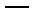
\includegraphics[scale=1]{\figpath/Model1_C2.pdf}\\%& 30 g/mol\\
			Butane & \ce{C4H10} & 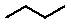
\includegraphics[scale=1]{\figpath/Model1_C4.pdf}\\%& 58 g/mol\\
			Hexane & \ce{C6H14} & 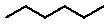
\includegraphics[scale=1]{\figpath/Model1_C6.pdf}\\%& 86 g/mol\\
			Octane & \ce{C8H18} & 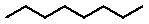
\includegraphics[scale=1]{\figpath/Model1_C8.pdf}\\%& 114 g/mol\\
			Decane & \ce{C10H22} & 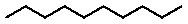
\includegraphics[scale=1]{\figpath/Model1_C10.pdf}\\%& 142 g/mol
		\end{tabular}
	\end{center}


\end{model}


\begin{ctqs}

	\question Between each line of the table and the next...
		\begin{enumerate}
			\item ... how many carbon atoms are added to the molecule?
			
				\begin{solution}[0.25in]
				2
				\end{solution}
				
			\item ... how many hydrogen atoms are added to the molecule?
			
				\begin{solution}[0.25in]
				4
				\end{solution}
				
		\end{enumerate}
		
	\question Explain, in 1-2 complete sentences, why we might say that this series of molecules consists of ``repeating'' \ce{C2H4} units.
			
				\begin{solution}[1.5in]
					If we ignore the methyl groups on the ends of the chains, we could divide each of the molecules up into a string of \ce{C2H2} units, with one new unit added as we go from one row of the table to the next.  Thus we can think of this series of molecules as consisting of \ce{C2H2} units repeating over and over until we make up the total number of units needed for the chain.
				\end{solution}
				
		
	\question Predict the chemical formula of the next logical entry in the table, and draw its structure.
			
				\begin{solution}[1in]
					The next entry would be \ce{C12H26}:
					
	\instructordisplay{\centerline{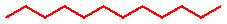
\includegraphics[width=0.3\textwidth]{\figpath/Model1_C12_answer.pdf}}}
				\end{solution}
		
	\question Consider a linear alkane with 100 carbon atoms. \label{\labelbase:ctq:100Calkane}
		\begin{enumerate}
			%\item What would the molecular weight of this molecule be?
			
			\item What would the chemical formula of this molecule be?
			
				\begin{solution}[1in]
					For an alkane with $n$ carbons, the number of hydrogens is $6+2(n-2) = 2n+2$.  Thus a molecule with 100 carbons would have formula\ce{C100H202}.
				\end{solution}
			
			\item Do you \emph{want} to try to draw the full structure of this molecule?  Why or why not?
			
				\begin{solution}[1.25in]
					No!  It would be super long, and really difficult to fit on the page.
				\end{solution}
		\end{enumerate}
\end{ctqs}

\begin{infobox}
	For convenience, large molecules with repeating structures are often abbreviated using the following notation:
	
	\centerline{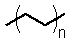
\includegraphics[scale=2]{\figpath/Model1_nrepeats.pdf}}
	
	Here, the repeat unit is enclosed in parentheses.  The repeat units are attached end-to-end, and the subscript $n$ indicates how many times this unit is repeated.  The portions outside of the parentheses are not part of the repeat unit, and indicate the chemical structure of the end-groups that ``cap'' the end of the molecule.
\end{infobox}

\begin{ctqs}
	\question Draw the full structure of the molecule shown in the following abbreviated structure: \label{\labelbase:ctq:abbrevbutane}
	
		\vspace{6pt}
		\centerline{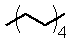
\includegraphics[scale=2]{\figpath/Model1_C10_abbreviated.pdf}}
		
		\begin{solution}[1.25in]
			\instructordisplay{
				\centerline{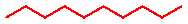
\includegraphics[width=0.3\textwidth]{\figpath/Model1_C10_answer.pdf}}
			}
		\end{solution}
	
	\question Propose an analogous abbreviated structure for the 100-carbon linear alkane described in CTQ \ref{\labelbase:ctq:100Calkane}: \label{\labelbase:ctq:abbrev100}
		
		\begin{solution}[0.75in]
			\instructordisplay{
				\centerline{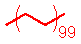
\includegraphics[width=0.1\textwidth]{\figpath/Model1_100C_abbreviated.pdf}}
			}
			Note: common student errors in this question include (1) missing the two carbons contained in the end groups and writing 50 in the subscript, or (2) forgetting that each repeat unit contains two carbon atoms and write 99 or 100 in the subscript.
		\end{solution}
	
	\question What is the chemical formula \emph{of the repeat unit} for the structures in CTQs \ref{\labelbase:ctq:abbrevbutane} and \ref{\labelbase:ctq:abbrev100}?
		
		\begin{solution}[0.75in]
			\ce{C2H4}
		\end{solution}
	
	\question What small molecule has the same chemical formula as this repeat unit?
		
		\begin{solution}[0.75in]
			Ethylene
			
			Note: many students will likely give the IUPAC name, ethene.  If they then get stuck on question 9, it can help to remind them that ``ethylene'' is the common name for this molecule.
		\end{solution}
	
\end{ctqs}

\begin{infobox}
	When the number of repeat units is large, we often describe molecules with repeating structures as \emph{polymers}.  The word polymer comes from Greek: \emph{poly} means ``many'', while \emph{meros} means ``parts''.  Thus, a \emph{polymer} is a molecule composed of \emph{many} (often identical) \emph{parts}.
\end{infobox}

\begin{ctqs}
	\question Why might we describe molecules of the form
	
		\centerline{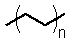
\includegraphics[scale=2]{\figpath/Model1_nrepeats.pdf}}
			
		as \emph{polyethylenes}?  Explain your answer in 1-2 complete sentences.
		
		\begin{solution}[2in]
			We refer to molecules of this form as polyethyelenes because they are made up of many ethylene repeat units.
		\end{solution}
\end{ctqs}

\clearpage
\begin{model}[Melting Points of Linear Hydrocarbons]
	\label{\labelbase:mdl:hydrocarbonmelting}

	The following plot shows the melting points of linear hydrocarbons with varying numbers of carbon atoms:
	
	\vspace{6pt}
	
	\centerline{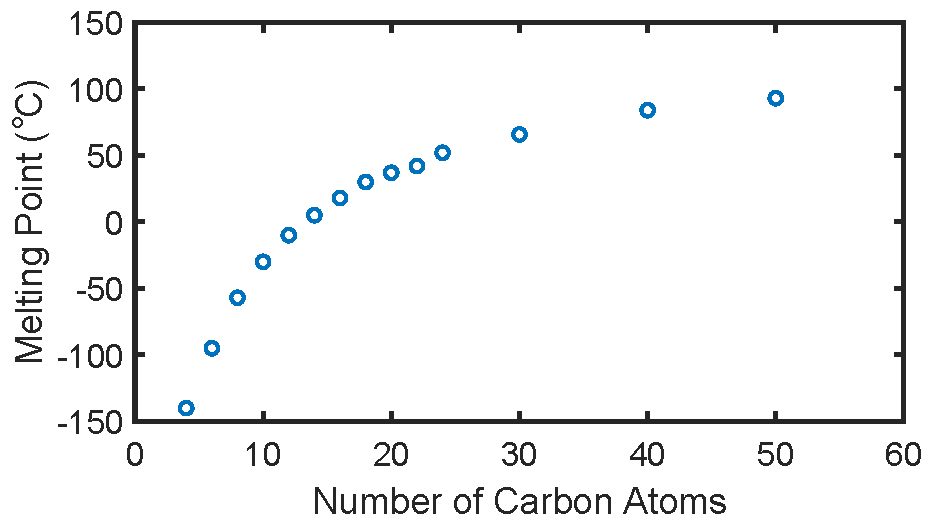
\includegraphics[width=0.7\textwidth]{\figpath/meltingpoints_cleaned.pdf}}
	
	\vspace{6pt}

\end{model}

\begin{ctqs}
	
	\question Consider a sample of ethane molecules.  What type(s) of interactions (e.g. covalent, ionic, hydrogen bonding, van der Waals, etc.) do you expect to govern interactions between these molecules?%, and why?  %Briefly explain your team's reasoning.
	
		\begin{solution}[0.5in]
			Ethane molecules are neither charged nor polar, so they most likely interact through van der Waals interactions.
			
			Note: some students may answer ``covalent''.  Remind these students that the question is asking about interactions \emph{between} chains, not the types of bonds \emph{within} chains.
		\end{solution}
	
	\question As the number of carbon atoms in the molecule increases, do you expect the strength of these intermolecular interactions increase, decrease, or stay the same? \label{\labelbase:ctq:interactionstrength}
	
		\begin{solution}[0.5in]
			Generally, van der Waals interactions increase in strength as molecules become larger and more polarizable, so the interactions between chains should become stronger as the number of carbon atoms in the chain increases.
		\end{solution}
	
	\question Using your answer to CTQ \ref{\labelbase:ctq:interactionstrength}, propose a possible origin for the trend observed in Model \ref{\labelbase:mdl:hydrocarbonmelting} in 1-2 complete sentences.
	
		\begin{solution}[2in]
			As the chains become longer, the interactions between molecules becomes stronger and it takes more energy to melt the material.  Thus, the melting temperature goes up.
		\end{solution}
	
	\question Based on the data presented in Model \ref{\labelbase:mdl:hydrocarbonmelting}, what do you expect to happen to the melting temperature as the number of carbon atoms gets very large (1000 or 10000 or more)?  Briefly explain your team's reasoning.
	
		\begin{solution}[2in]
		
			The data look like they are beginning to level off as the number of carbon atoms increases.  Assuming this trend continues, the melting temperature for very large hydrocarbons is likely to limit somewhere between 100 and 150~${}^\circ$C. 
		\end{solution}
	
	\question The melting temperature of polyethylene is typically quoted as approximately 120~${}^\circ$C.  In your group's judgment, how many carbon atoms are necessary before the melting behavior begins to ``look'' more like the polymer than like a small molecule?  Explain your choice in 2-3 complete sentences. \label{\labelbase:ctq:npolymer}
	
		\begin{solution}[2in]
		
			Student answers will likely vary.  Some may say that it requires 100-500 carbon atoms, because that is where the curve will probably begin to approach 120~${}^\circ$C.  Others may say that it only taks 15-20 carbon atoms, because that is where the slope of the curve really starts to decrease.
			
			In discussion, it is worth emphasizing that the properties of polymers usually change continuously with chain length, and there is no distinct ``cutoff'' that determines when we can start calling something a polymer.  In \emph{practice}, molecules with fewer than 10 repeat units rarely behave like polymers, and are instead referred to as oligomers, while molecules with more than 100 repeat units are usually solidly ``polymer-like''; in between these limits, whether you will see polymer-like or molecule-like behavior depends a lot on which property you are measuring.
			
			(One aspect of this problem is addressed in Exercise 1 of Activity 2, which asks students to consider when end groups do and do not matter on polymer chains.)
		\end{solution}
	
	%\question How many repeat units does this number of carbons correspond to?
	
	%	\begin{solution}[0.5in]
	%	\end{solution}
			
\end{ctqs}

		

\begin{exercises}

	\exercise How many repeat units does the number of carbon atoms you identified in CTQ \ref{\labelbase:ctq:npolymer} correspond to?
	
		\begin{solution}
		
			Student answers will vary, but for $n$ carbon atoms, the corresponding number of repeat units is $(n-2)/2$.
			
		\end{solution}

	\exercise In this class, we will primarily use the word ``polymer'' to describe large molecules with repeating structures.  Another word commonly used in this field, however, is ``macromolecule''.  Why is this also a reasonable term for describing this class of molecules, and does it capture any important features that are missed by the word ``polymer''?
	
		\begin{solution}
			``Macromolecule'' literally means ``large molecule''.  This term is reasonable for describing polymers because they are, in essence, very large molecules, and it emphasizes that the size is the primary feature that distinguishes them from most familiar small molecules.
			
			In practice, we generally use the terms ``macromolecule'' and ``polymer'' interchangeably.  However, it is worth noting that macromolecule is, in some ways, less specific than ``polymer''; a macromolecule can refer to any large molecule, even if it is not made up of repeating parts.  On the other hand, the word ``molecule'' typically refers to collections of atoms that are covalently bonded together, whereas polymer (``many parts'') could feasibly just refer to a collection of loosely associated molecular units, or units that are held together by hydrogen bonds, metal coordination bonds, or other types of non-covalent bonds.  Thus the two terms, while getting at many of the same ideas, are not strictly identical.
		\end{solution}
	
\end{exercises}


%\begin{problems}

%	\problem First exercise
%	\problem Second exercise
	
%\end{problems}


	
\end{activity}
		%%%%%%%%%%%%%%%%%%%%%%%%%%%%%%%%%%%%%%%%%
%
% (c) 2020 by Jennifer Laaser
%
% This work is licensed under the Creative Commons Attribution-NonCommercial-ShareAlike 4.0 International License. To view a copy of this license, visit http://creativecommons.org/licenses/by-nc-sa/4.0/ or send a letter to Creative Commons, PO Box 1866, Mountain View, CA 94042, USA.
%
% The current source for these materials is accessible on Github: https://github.com/jlaaser/pogil-polymers
%
%%%%%%%%%%%%%%%%%%%%%%%%%%%%%%%%%%%%%%%%%

\renewcommand{\figpath}{content/intro/size-and-complexity/figs}
\renewcommand{\labelbase}{size-and-complexity}

\begin{activity}[With Increasing Size Comes Increasing Complexity]

\begin{instructornotes}

	This activity introduces students to key concepts related to the size and molecular weight of polymer molecules, and conformational flexibility.
	
	After completing this activity, students will be able to:
			\begin{enumerate}
				\item Calculate the molecular weight of a polymer, given the number of repeat units and molecular weight of each repeat (and calculate number of repeat units given molecular weight)
				\item Estimate the physical extent of a polymer that is (a) fully extended, (b) fully collapsed, or (c) somewhere inbetween
				\item Estimate the number of conformations available for a single polymer molecule
			\end{enumerate}
			
	\subsection*{Activity summary:}
	\begin{itemize}
		\item \textbf{Activity type:} Learning Cycle
		\item \textbf{Content goals:} Introduction to polymers
		\item \textbf{Process goals:} %https://pogil.org/uploads/attachments/cj54b5yts006cklx4hh758htf-process-skills-official-pogil-list-2015-original.pdf
			written communication, critical thinking, information processing
		\item \textbf{Duration:} 35-40 minutes, including class discussion
		\item \textbf{Instructor preparation required:} none beyond knowledge of relevant content
		\item \textbf{Related textbook chapters:}
			\begin{itemize}
				\item \emph{Polymer Chemistry} (Hiemenz \& Lodge): section 1.2
			\end{itemize}
		%\item \textbf{Facilitation notes:}
		%	\begin{itemize}
		%		\item \dots
		%	\end{itemize}
	\end{itemize}
	
\end{instructornotes}




\begin{model}[Molecular Weight and Degree of Polymerization]
\label{\labelbase:mdl:polyethyleneMW}

	The structure of polyethylene is shown below:

	\vspace{6pt}
	\centerline{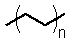
\includegraphics[scale=2]{\figpath/Model1_nrepeats.pdf}}
	\vspace{6pt}
	
	The repeat unit has a chemical formula of \ce{C2H4} and a molecular weight of 28 g/mol.

\end{model}


\begin{ctqs}

	\question Consider a molecule of polyethylene with 100 repeat units.  What would the molecular weight of this molecule be?
			
				\emph{Note: for the purposes of this activity, you may ignore the \ce{CH3} end groups on the chain, and only consider the atoms in the repeat units.}
	
		\begin{solution}[1.5in]
		
			\begin{equation*}
				\left(100\text{ repeat units}\right)\left(\frac{28\text{ g/mol}}{1\text{ repeat unit}}\right) = 2800\text{ g/mol}
			\end{equation*}
		\end{solution}
				
	\question Conversely, consider a molecule of polyethylene with a molecular weight of 700~kg/mol.  Approximately how many repeat units would this chain contain? \label{\labelbase:ctq:700kgPE}
	
		\begin{solution}[1.5in]
		\begin{equation*}
			\left(\frac{700\text{ kg}}{1\text{ mol}}\right)
			\left(\frac{1000\text{ g}}{1\text{ kg}}\right)
			\left(\frac{1\text{ repeat unit}}{28\text{ g/mol}}\right)
			= 25000\text{ repeat units}
		\end{equation*}
		
			As a point of interest, this is in the ballpark for commercial HDPE and LDPE, which typically have degrees of polymerization between 10000 and 100000.
		\end{solution}
	
\end{ctqs}

\begin{infobox}

	Polymer chains are typically synthesized from small molecules called \emph{monomers}.  The number of monomers that make up a polymer chain, $N$, is referred to as the \emph{degree of polymerization}.
	
	For polyethylene, each \ce{C2H4} repeat unit corresponds to exactly one ethylene monomer.

\end{infobox}

\begin{ctqs}
		
	\question What would the molecular weight of a polyethylene molecule made up of $N$ monomers be?
	
		\begin{solution}[1in]
			$28 N$ g/mol
		\end{solution}
		
	\question More generally, suppose a polymer chain is made up of $N$ monomers that each have molecular weight $M_0$.  What would the molecular weight of this polymer be?
	
		\begin{solution}[1in]
			$M_0 N$
		\end{solution}
	
	\question Explain, in 1-2 complete sentences, how you could calculate each of the following:
	
		\begin{enumerate}
			\item The molecular weight of a polymer, if you knew the degree of polymerization and the molecular weight of each monomer:
	
		\begin{solution}[1.75in]
			To obtain the molecular weight of the polymer, you would multiply the degree of polymerization by the molecular weight of the monomer ($M = M_0 N$).
		\end{solution}
			
			\item The degree of polymerization, if you knew the molecular weight of the polymer and the molecular weight of each monomer:
	
		\begin{solution}[1.75in]
			To obtain the degree of polymerization, you would divide the molecular weight of the polymer by the molecular weight of the monomer ($N = \frac{M}{M_0}$).
		\end{solution}
		
		\end{enumerate}
	
\end{ctqs}



\begin{model}[Sizes of Polymer Chains]
	\label{\labelbase:mdl:polyethylenesize}
	
	Carbon-carbon single bonds are typically approximately 1.5~\AA\ long.  Because the bond angle in linear alkanes is approximately 109.5${}^\circ$, every two carbon-carbon bonds contributes approximately 0.25~nm to the length of a polymer chain when it is in its fully extended conformation:
	
	\vspace{6pt}
	\centerline{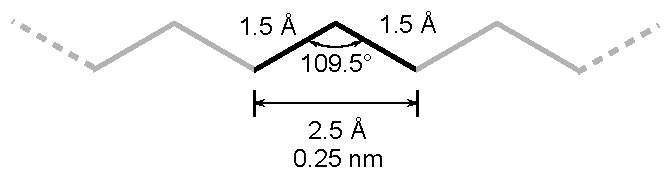
\includegraphics[width=0.7\textwidth]{\figpath/Model2_extendedchain.pdf}}

\end{model}

\begin{ctqs}

	\question How many carbon-carbon bonds does each repeat unit contribute to a polyethylene chain?
	
		\emph{Note: make sure to pay attention not only to the bond in the middle of each repeat unit, but also the bonds that connect different repeat units - how should you count these?}
		
		\begin{solution}[1in]
			2
		\end{solution}
	
	\question How many carbon-carbon bonds would the 700~kg/mol polyethylene molecule in CTQ \ref{\labelbase:ctq:700kgPE} contain?
		
		\begin{solution}[1in]
			$2(25000)\approx 50000$
		\end{solution}
	
	\question Using your answer to the previous question, and the information in Model \ref{\labelbase:mdl:polyethylenesize}, calculate the expected length of this molecule in its fully extended conformation. \label{\labelbase:ctq:extendedPE}
		
		\begin{solution}[2in]
			\begin{equation*}
				\left(50000\text{ C-C bonds}\right)\left(\frac{0.25\text{ nm}}{2\text{ C-C bonds}}\right) = 6250\text{ nm} = 6.25~\mu\text{m}
			\end{equation*}
			
			(Note: some students may leave out the factor of 2 in the denominator in this problem, but will likely self-correct quickly during discussion.)
			
			Students may find it interesting to consider that this is comparable to the dimensions of a red blood cell - it is very large for a single molecule!
		\end{solution}
	
	\question Suppose that instead of stretching the chain out, we collapsed it into a sphere with the same density as bulk polyethylene (approximately 0.95~g/cm\textsuperscript{3}).  What would the radius of this sphere be? \label{\labelbase:ctq:collapsedPE}
	
		\emph{Hint: you'll need to find the mass of a single chain, and then use the density to calculate how much volume it takes up.  You'll probably find it useful to remember that Avogadro's number is approximately 6.022$\times 10^{23}$, and the volume of a sphere of radius $R$ is $\frac{4}{3}\pi R^3$.}
		
		\begin{solution}[3.75in]
			First, let's calculate the volume of a single polymer chain:
			\begin{equation*}
				\left(\frac{700\text{ kg}}{1\text{ mol}}\right)
				\left(\frac{1\text{ mol}}{6.022\times10^{23}\text{ molecules}}\right)
				\left(\frac{1\text{ cm}^3}{0.95\text{ g}}\right)
				\left(\frac{1000\text{ g}}{1\text{ kg}}\right)
				= 1.22 \times 10^{-18}\text{ cm}^3
			\end{equation*}
			Rearranging the equation for the volume of a sphere to solve for radius, we obtain
			\begin{equation*}
				R=\sqrt[3]{\frac{3 V}{4\pi}} = \sqrt[3]{\frac{3 \left(1.22 \times 10^{-18}\text{ cm}^3\right)}{4\pi}} = 6.6 \times 10^{-7}\text{ cm} = 6.6\text{ nm}
			\end{equation*}
			This is three orders of magnitude smaller than the fully extended chain discussed in the previous problem!
		\end{solution}
		
	\question In practice, a 700~g/mol polyethylene chain will typically have a spatial extent on the order of 40~nm.  
	
		\begin{enumerate}
			\item Is this closer to your estimate from CTQ \ref{\labelbase:ctq:extendedPE} or CTQ \ref{\labelbase:ctq:collapsedPE}?
			
				\begin{solution}[0.5in]\instructordisplay{
					This value is closer to the radius of the collapsed chain calculated in CTQ \ref{\labelbase:ctq:collapsedPE}.
				}\end{solution}
			
			\item What does your answer tell you about whether polymer chains are typically more extended or more collapsed?  Explain your answer in 1-2 complete sentences.
			
				\begin{solution}[1.75in]
					This result suggests that polymer chains are typically more collapsed than extended.  However, because the spatial extent is still almost an order of magnitude larger than expected for the fully collapsed globule, the chain can't be fully collapsed, and is likely more of a loose coil.
				\end{solution}
			
		\end{enumerate}
		
\end{ctqs}



\begin{model}[Conformations of Polymer Chains]
	\label{\labelbase:mdl:conformations}

	As seen in Model \ref{\labelbase:mdl:polyethylenesize}, polymer chains may have many different conformations.  In fact, each carbon-carbon bond in polyethylene can take one of three different conformations:
	
	\vspace{6pt}
	\centerline{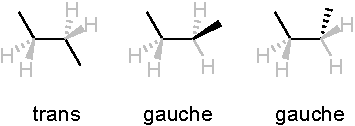
\includegraphics[width=0.5\textwidth]{\figpath/Model3_conformations.pdf}}
	
	As a result, the total number of conformations of a molecule with $n$ carbon-carbon bonds is $3^n$.

\end{model}

\begin{ctqs}

	\question How many possible conformations does the 700~kg/mol molecule of polyethylene considered earlier in this activity have?
	
		\begin{solution}[1in]
			\begin{equation*}
				3^{\text{\# of C-C bonds}} = 3^{50000} \approx 10^{23850}
			\end{equation*}
		\end{solution}
	
	\question 1~kg of 700~kg/mol polyethylene would contain approximately $9\times 10^{20}$ molecules.  Using this information, critique or defend the following statement in 2-3 complete sentences:
	
		\emph{``On average, a polymer sample will contain many molecules in each conformation.''}
	
		\begin{solution}[2.5in]
		
			This statement is false.  The number of possible conformations is much, much larger than the number of molecules in the sample, by thousands of orders of magnitude.  Thus the polymer chains the sample almost certainly all have different conformations, and it is very unlikely that any two are the same.
		\end{solution}
		
\end{ctqs}


\begin{exercises}

	\exercise In Model \ref{\labelbase:mdl:polyethyleneMW} (and the rest of this activity), we ignored the molecular weight of the end groups.  To determine whether or not this was a reasonable approximation, do the following:
	
		\begin{enumerate}
			
			\item Derive a formula for the molecular weight of a polyethylene molecule containing $N$ \ce{C2H4} repeat units and two \ce{CH3} end groups.
			
				\begin{solution}\instructordisplay{
					Each \ce{C2H4} repeat has a molecular weight of 28 g/mol, while each \ce{CH3} end group has a molecular weight of 15 g/mol, so the correct formula is (28*N + 2*15) g/mol.
				}\end{solution}
			
			\item Derive a formula for the molecular weight of a polyethylene molecule containing only $N$ \ce{C2H4} repeat units (i.e. without counting the end groups).
			
				\begin{solution}\instructordisplay{
					Using the same approach as in part (a), but neglecting the end groups, the molecular weight is 28*$N$ g/mol.
				}\end{solution}
			
			\item Calculate the molecular weight obtained from each formula for $N=10$, $N=20$, $N=50$, $N=100$, $N=200$, and $N=500$. For each value of $N$, what is the percent error in the estimate obtained when you ignore the end groups, and above what degree of polymerization would you judge this error to be negligible?
			
				\begin{solution}\instructordisplay{
					The calculated values are:
					
					\begin{center}
						\begin{tabular}{cccc}
						\hline
N   & MW with end groups (g/mol) & MW without end groups (g/mol) & \% error \\\hline
10  & 310                        & 280                           & -9.7     \\
20  & 590                        & 560                           & -5.1     \\
50  & 1430                       & 1400                          & -2.1     \\
100 & 2830                       & 2800                          & -1.1     \\
200 & 5630                       & 5600                          & -0.5     \\
500 & 14030                      & 1400                          & -0.2  
\\\hline  
\end{tabular}
					\end{center}
					
					The N value above which students judge the correction to be negligible depends on how much error they are willing to accept, but using 1\% as a good rule of thumb, the correction is negligible when the chains have 100 or more repeat units.

Note: all of the \% errors should be negative - the molecular weight when end groups are ignored is always lower than the correct molecular weight.

				}\end{solution}
			
		\end{enumerate}
		
	\exercise Summarize, in your own words, the key ways in which polymers differ from small molecules.
	
		\begin{solution}\instructordisplay{
			The key ways in which polymers differ from small molecules include:

\begin{enumerate}
	\item Their physical size: polymers have physical sizes ranging from a few nanometers, in their fully collapsed states, to several microns, in their fully extended conformations.  This is much larger than - and a much larger range than - small molecules.
	\item Their molecular weights: polymers have molecular weights in the thousands to millions of grams per mole, while small molecules rarely have molecular weights greater than a few hundred grams per mole.  The large molecular weights mean that intermolecular interactions between polymers are typically strong, which affects their physical properties (e.g. state of matter, solubility, viscosity, etc. - see previous Activity).
	\item Their number of accessible conformations: polymer molecules typically have so many conformations that it is impossible to enumerate them or to have more than one of each conformation in a sample.  Small molecules, on the other hand, typically only have a handful of conformations that can be enumerated exactly.
\end{enumerate}

Although not addressed in this Activity, once students are introduced to the concepts of dispersity, composition, tacticity, and topology they should additionally recognize that polymers also differ from small molecules in their heterogeneity: polymer samples can contain molecules with different molecular weights, different compositions, different stereochemistries, and potentially different connectivity.  This heterogeneity means that we always have to think about polymers in terms of averages over large numbers of molecules rather than as a single well-defined structure.

		}\end{solution}
	
\end{exercises}


%\begin{problems}

%	\problem First exercise
%	\problem Second exercise
	
%\end{problems}


	
\end{activity}
		%%%%%%%%%%%%%%%%%%%%%%%%%%%%%%%%%%%%%%%%%
%
% (c) 2023 by Jennifer Laaser
%
% This work is licensed under the Creative Commons Attribution-NonCommercial-ShareAlike 4.0 International License. To view a copy of this license, visit http://creativecommons.org/licenses/by-nc-sa/4.0/ or send a letter to Creative Commons, PO Box 1866, Mountain View, CA 94042, USA.
%
% The current source for these materials is accessible on Github: https://github.com/jlaaser/pogil-polymers
%
%%%%%%%%%%%%%%%%%%%%%%%%%%%%%%%%%%%%%%%%%

\renewcommand{\figpath}{content/intro/nomenclature/figs}
\renewcommand{\labelbase}{nomenclature}

\begin{activity}{Polymer Nomenclature}

\begin{instructornotes}

	This activity introduces students to key concepts related to the nomenclature of polymers.
	
	After completing this activity, students will be able to:
			\begin{enumerate}
				\item \dots
			\end{enumerate}
			
	\subsection*{Activity summary:}
	\begin{itemize}
		\item \textbf{Activity type:} Learning Cycle
		\item \textbf{Content goals:} See above
		\item \textbf{Process goals:} %https://pogil.org/uploads/attachments/cj54b5yts006cklx4hh758htf-process-skills-official-pogil-list-2015-original.pdf
			\begin{itemize}
				\item Interpreting chemical structures
				\item Written and oral communication of reasoning
			\end{itemize}
		\item \textbf{Duration:} TBD
		\item \textbf{Instructor preparation required:} none beyond knowledge of relevant content
		\item \textbf{Related textbook chapters:}
			\begin{itemize}
				\item \emph{Polymer Chemistry} (Hiemenz \& Lodge), 2nd ed.: sections 1.3, 1.5, and 1.6
				\item \emph{Introduction to Polymres} (Young \& Lovell), 3rd ed.: section 1.2
			\end{itemize}
		%\item \textbf{Facilitation notes:}
		%	\begin{itemize}
		%		\item \dots
		%	\end{itemize}
	\end{itemize}

\end{instructornotes}

	%\textbf{Focus question:} Put a central question for the students to consider through this exercise here.

\begin{model}[Chain Chemistry]
\label{\labelbase:mdl:backsideend}

	When describing the chemistry of polymer chains, the three most important components of the molecule are the \emph{backbone}, the \emph{sidechains}, and the \emph{end groups}, as shown schematically below:
	
	\centerline{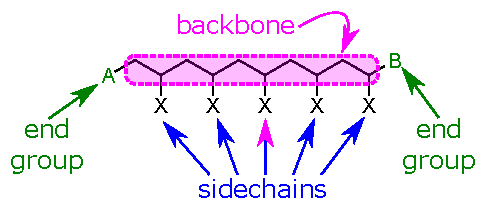
\includegraphics[width=0.5\textwidth]{\figpath/Model1_schematic.pdf}}

\end{model}


\begin{ctqs}

	\question Which of these components (backbone, sidechains, or end groups)...
	
		\begin{enumerate}
			\item ... contain the bonds and/or functional groups that make up the ``main chain'' that spans from one end of the polymer to the other?
			
				\begin{solution}[0.25in]
					backbone
				\end{solution}
			
			\item ... contain the functional groups that are attached to every repeat unit but are not part of unbroken string of bonds connecting one end of the polymer to the other?
			
				\begin{solution}[0.25in]
					sidechains
				\end{solution}
			
			\item ... ``cap'' the ends of the polymer chain?
			
				\begin{solution}[0.25in]
					end groups
				\end{solution}
				
		\end{enumerate}
		
	\question The structure of a polystyrene chain is given below:
	
		\centerline{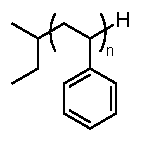
\includegraphics[width=0.15\textwidth]{\figpath/Model1_PS}}
	
		For this polymer, identify and sketch the structures of...
		\begin{enumerate}
			\item the backbone:
			
				\begin{solution}[0.75in]\studentdisplay{
					~
				}\instructordisplay{
					The backbone contains the string of C-C bonds highlighted below:
					
					\centerline{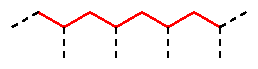
\includegraphics[width=0.3\textwidth]{\figpath/Model1_PS_backbone_soln}}
				}\end{solution}
			
			\item the sidechains:
			
				\begin{solution}[0.5in]\studentdisplay{
					~
				}\instructordisplay{
					The sidechains consist of the aromatic rings, as highlighted below:
					
					\centerline{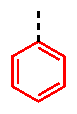
\includegraphics[width=0.075\textwidth]{\figpath/Model1_PS_sidechain_soln}}
				}\end{solution}
			
			\item the end groups:
			
				\begin{solution}[0.5in]\studentdisplay{
					~
				}\instructordisplay{
					The end groups are a sec-butyl group (left) and a hydrogen atom (right), as indicated below:
					
					\centerline{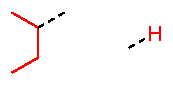
\includegraphics[width=0.2\textwidth]{\figpath/Model1_PS_endgrps_soln}}
				}\end{solution}
			
			
		\end{enumerate}
		
	\question Polystyrene is produced from the styrene monomer,
	
		\centerline{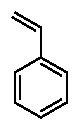
\includegraphics[width=0.1\textwidth]{\figpath/Model1_styrene}}
	
		\begin{enumerate}
			\item Upon polymerization, which bond from this monomer is incorporated into the backbone of the polymer chain?
			
				\begin{solution}[0.5in]
				
					The double bond is converted to a single bond and incorporated into the backbone of the chain.
					
				\end{solution}
				
			\item How is the structure of the repeat unit related to the structure of this monomer?
			
				\begin{solution}[0.5in]
				
					They have the same chemical formula and connectivity of the atoms, but the double bond in the monomer is replaced by a single bond in the polymer, and new bonds are formed to connect the monomer to the adjacent repeat units.
					
				\end{solution}
				
			\item How is the name of the polymer related to the name of this monomer?
			
				\begin{solution}[0.5in]
				
					The name of the polymer is just poly( name of the monomer ).
					
				\end{solution}
				
		\end{enumerate}
		
	\question Two other common polymers, and the monomers used to produce them, are shown below:
	
		\centerline{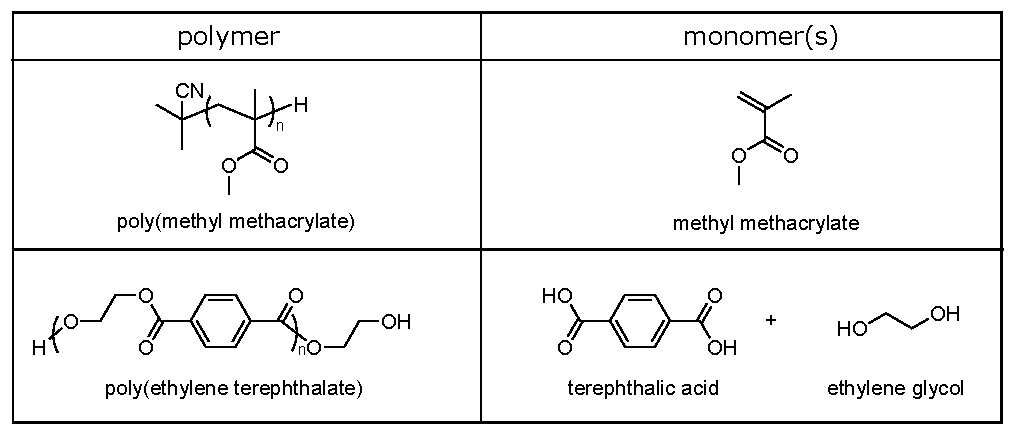
\includegraphics[width=0.8\textwidth]{\figpath/Model1_polymermonomertable}}
		
		Based on these structures, critique or defend each of the following statements in 2-3 complete sentences:
		
		\begin{enumerate}
			\item \emph{``Polymer chains always have backbones consisting of only C-C single bonds.''}
			
				\begin{solution}[1.5in]
					FALSE - clearly not true for PET!
				\end{solution}
			
			\item \emph{``Polymers are always named for the monomer from which they are produced.''}
			
				\begin{solution}[1.5in]
					FALSE - also clearly not true for PET!
				\end{solution}
			
		\end{enumerate}

\end{ctqs}

\begin{infobox}
	Polymers are typically named for their ``constituent repeat unit.''
\end{infobox}

\begin{ctqs}

	\question The structure of ethylene terephthalate is shown below:
	
		\centerline{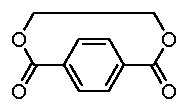
\includegraphics[width=0.2\textwidth]{\figpath/Model1_ethyleneterephthalate}}
		
		Is this structure consistent with the rule given in the above information box?  Briefly explain your group's reasoning.
		
		\begin{solution}[0.75in]
			Yes, it is.  This molecule has the same structure as the repeat unit of the poly(ethylene terephthalate) molecule, with only one bond needing to be broken/re-formed to link to adjacent repeat units.
			
			Note that IUPAC specifies clear rules for how the constituent repeat unit is named, which the above examples do not follow - we have given the ``common names'' for the repeat units rather than their IUPAC names.  See DOI 10.1351/PAC-REP-12-03-05 for a brief guide to IUPAC nomenclature.
		\end{solution}

\end{ctqs}


\clearpage

%\begin{model}[Architecture]

%	The polymers shown in Model \ref{\labelbase:mdl:backsideend} were all \emph{linear} polymers, in which the backbone makes a single unbroken line from one end of the molecule to the other.  However, the backbone can also have more complex \emph{architectures}, some of which are illustrated below:
	
%	FIG

%\end{model}

%\begin{ctqs}

%	\question ...
	
%\end{ctqs}


\begin{model}[Composition]
\label{\labelbase:mdl:composition}

	The polymers shown in Model \ref{\labelbase:mdl:backsideend} contain only one type of repeat unit.  However, it is also possible to produce polymers with multiple types of repeat units.  These polymers are usually classified in terms of how many distinct repeat units they contain, and how those repeat units are distributed throughout the chain.
	
	Several common classes of polymers are illustrated below:
	
	{\renewcommand{\arraystretch}{1.75}
	\begin{tabular}{m{0.78in}m{2in}m{2.5in}}
		\hline
		Classification & Repeat Unit Distribution & Example\\
		\hline
		Homopolymer & AAAAAAAAAAAAAAAAAA & 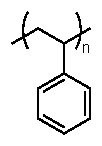
\includegraphics[width=0.4in]{\figpath/Model2_PS} ~~ poly(styrene) \\\hline
		Statistical Copolymer & ABBBABAABBAAAABBAB & 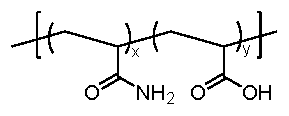
\includegraphics[width=1.25in]{\figpath/Model2_PAmAA} \newline poly(acrylamide-\emph{stat}-acrylic acid)\\\hline
		Alternating Copolymer & ABABABABABABABABAB & 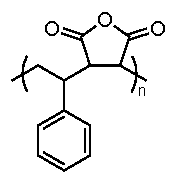
\includegraphics[width=0.75in]{\figpath/Model2_PSaltMA} \newline poly(styrene-\emph{alt}-maleic anhydride)\\\hline
		Diblock Copolymer & AAAAAAAAABBBBBBBBB & 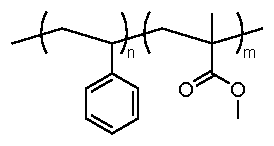
\includegraphics[width=1.25in]{\figpath/Model2_PSblockPMMA} \newline poly(styrene)-\emph{block}-poly(methyl methacrylate)\\\hline
		Triblock Copolymer & AAAAAABBBBBBAAAAAA & 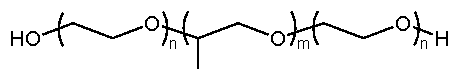
\includegraphics[width=2in]{\figpath/Model2_pluronic} \newline poly(ethylene oxide)-\emph{block}-poly(propyl\-ene oxide)-\emph{block}-poly(ethylene oxide) \\\hline
		Statistical Terpolymer & ABBCABACCCBCAABACB & 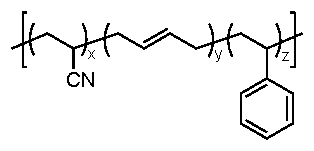
\includegraphics[width=1.5in]{\figpath/Model2_ABS} \newline poly(acrylonitrile-\emph{stat}-butadiene-\emph{stat}-styrene) \\\hline
		Graft Copolymer & 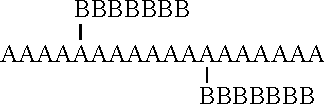
\includegraphics[width=1.75in]{\figpath/Model2_graftschematic} & 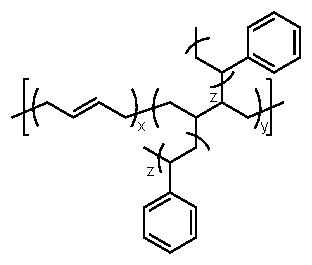
\includegraphics[width=1.25in]{\figpath/Model2_PBgPS} \newline poly(butadiene)-\emph{graft}-poly(styrene) 
	\end{tabular}
	}

\end{model}

\begin{ctqs}

	\question How many types of repeat units are included in...
	
		\begin{enumerate}
			\item ... homopolymers?
			
				\begin{solution}[0.25in]
				\end{solution}
			
			\item ... copolymers?
			
				\begin{solution}[0.25in]
				\end{solution}
			
			\item ... terpolymers?
			
				\begin{solution}[0.25in]
				\end{solution}
			
		\end{enumerate}
	
	\question For block copolymers, which part of the classification name indicates the number of polymer ``blocks''?
			
				\begin{solution}[0.5in]
				\end{solution}

	\question Compare the statistical, alternating, and diblock copolymers shown in the above table.
	
		\begin{enumerate}
		
			\item What are the key differences in how the repeat units are arranged in these three types of polymers?  Summarize your group's findings in 1-2 complete sentences.
			
				\begin{solution}[1.75in]
				\end{solution}
	
			\item How is the placement of the parentheses and/or brackets in the skeletal structures in the right-hand column used to indicate how the repeat units are arranged in these three types of polymers?  Summarize your group's findings in 1-2 complete sentences.
			
				\begin{solution}[1.75in]
				\end{solution}
			
		\end{enumerate}
		
	\question Classify each of the following polymers.  
	
		(\emph{Challenge: if you have extra time, see if you can propose a formal name for each structure, too!})
	
		\begin{enumerate}
			\item \text{}\\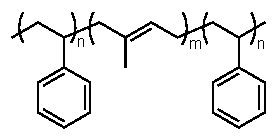
\includegraphics[width=0.25\textwidth]{\figpath/Model2_SBS}
			
				\begin{solution}[0.25in]
					triblock copolymer (poly(styrene)-\emph{block}-poly(butadiene)-\emph{block}-poly(styrene))
				\end{solution}
			
			\item \text{}\\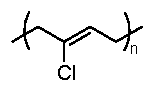
\includegraphics[width=0.15\textwidth]{\figpath/Model2_neoprene}
			
				\begin{solution}[0.25in]
					homopolymer (poly(chloroprene))
				\end{solution}
			
			\item \text{}\\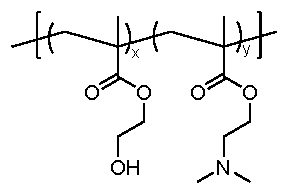
\includegraphics[width=0.25\textwidth]{\figpath/Model2_HEMAstatDMAEMA}
			
				\begin{solution}[0.25in]
					statistical copolymer (poly(hydroxyethyl methacrylate - \emph{stat} - dimethylaminoethyl methacrylate))
				\end{solution}
			}
		\end{enumerate}
		
	\question Propose a possible sequence of a triblock copolymer consisting of repeat units A, B, and C.
	
		\begin{solution}[0.5in]
		\end{solution}
	
	\question Draw the skeletal structure of a statistical copolymer of styrene and acrylonitrile.
	
		\begin{solution}[1in]
		\end{solution}
	
\end{ctqs}


\clearpage
\begin{model}[Isomerism]

	Here is a second model for students to consider.

\end{model}

\begin{ctqs}

	\question First question?
	
		\begin{solution}
		\end{solution}
	
	\question Second question?
	
		\begin{solution}
		
			Here's a solution environment that doesn't have a height set, but does have content.
			
			(The previous solution environment has no height and no content.)		
		
		\end{solution}
\end{ctqs}

		
\begin{infobox}
	Here is some useful information that might help the students with the next few critical thinking questions.
	In some cases, it might include an equation:
	\begin{equation*}
		a^2 + b^2 = c^2
	\end{equation*}
	or even more than one equation:
	\begin{equation*}
		x=\frac{-b \pm \sqrt{b^2-4ac}}{2a}
	\end{equation*}
\end{infobox}

\begin{ctqs}

	\question First question?
		\begin{solution}[1in]
		\end{solution}
	
	\question Second question?
		\begin{solution}[1in]
		\end{solution}
\end{ctqs}



\begin{exercises}

	\exercise Poly(styrene) is an example of a ``vinyl-type'' polymer.  Vinyl-type polymers have the following general structure, as shown in Model \ref{\labelbase:mdl:backsideend}:
	
		IMAGE
		
		\begin{enumerate}
		
			\item Propose the structure of the monomer that is most likely used to produce this polymer.
			
				\emph{Hint: try replacing the aromatic ring in the structures shown in CTQs nnn and mmm with an ``X''!}
			
			\item Based on the structure you drew, explain, in 1-2 complete sentences, why these polymers are reasonably described as ``vinyl-type'' polymers.
			
		\end{enumerate}
		
	%\exercise Something about IUPAC nomenclature: 10.1351/PAC-REP-12-03-05
		
	%\exercise structure of kraton rubbers (SBS triblocks that then get hydrogenated?)
	
	%\exercise something about random vs statistical copolymers?
		
	\exercise Second exercise
	
\end{exercises}

	
\end{activity}
		%%%%%%%%%%%%%%%%%%%%%%%%%%%%%%%%%%%%%%%%%
%
% (c) 2018 by Jennifer Laaser
%
% This work is licensed under the Creative Commons Attribution-NonCommercial-ShareAlike 4.0 International License. To view a copy of this license, visit http://creativecommons.org/licenses/by-nc-sa/4.0/ or send a letter to Creative Commons, PO Box 1866, Mountain View, CA 94042, USA.
%
% The current source for these materials is accessible on Github: https://github.com/jlaaser/pogil-polymers
%
%%%%%%%%%%%%%%%%%%%%%%%%%%%%%%%%%%%%%%%%%

\renewcommand{\figpath}{content/intro/M-and-D/figs}
\renewcommand{\labelbase}{M-and-D}

\begin{activity}{Molecular Weight and Dispersity}
\label{\labelbase}

\begin{instructornotes}

	This activity introduces students to key concepts related to the molecular weight and dispersity of polymer chains.
	
	After completing this activity, students will be able to:
			\begin{enumerate}
				\item Calculate the number-average and weight-average molecular weights of a polymer sample
				\item Calculate the dispersity of a polymer sample
				\item Interpret the dispersity of a polymer sample in terms of its molecular weight distribution
			\end{enumerate}
			
	\subsection*{Activity summary:}
	\begin{itemize}
		\item \textbf{Activity type:} Learning Cycle
		\item \textbf{Content goals:} See above
		\item \textbf{Process goals:} %https://pogil.org/uploads/attachments/cj54b5yts006cklx4hh758htf-process-skills-official-pogil-list-2015-original.pdf
			\begin{itemize}
				\item Analyzing quantitative data
				\item Interpreting data to infer a general trend
				\item Written and oral communication of reasoning
			\end{itemize}
		\item \textbf{Duration:} 30 min, including time for discussion
		\item \textbf{Instructor preparation required:} none beyond knowledge of relevant content
		\item \textbf{Related textbook chapters:}
			\begin{itemize}
				\item \emph{Polymer Chemistry} (Hiemenz \& Lodge), 2nd ed.: section 1.7
				\item \emph{Introduction to Polymers} (Young \& Lovell), 3rd ed.: section 1.3
			\end{itemize}
	\end{itemize}

\end{instructornotes}

\begin{model}[Calculating Average Chain Lengths]
\label{\labelbase:mdl:MNandMW}

	Most polymer samples contain a distribution of chains of different lengths.  Typically, we want to know what the \emph{average} chain length is.  However, there is more than one way that we can compute an average.
	
	Consider the following set of polymer chains:
	
		\vspace{6pt}
		\centerline{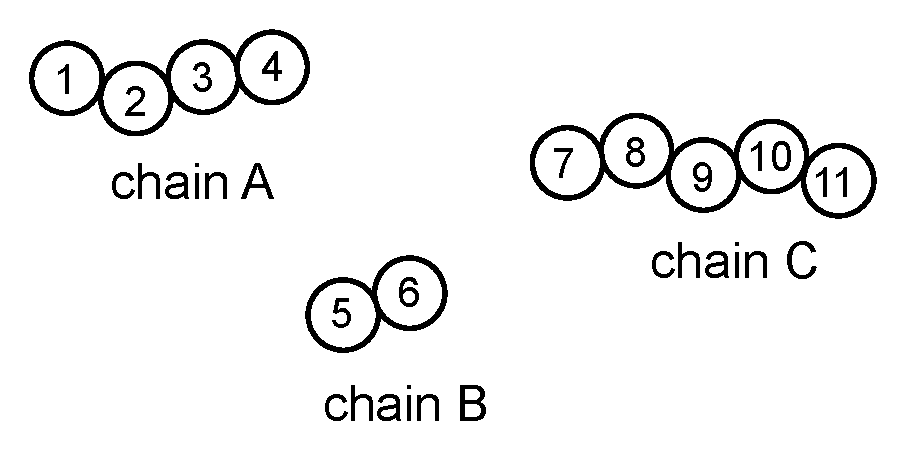
\includegraphics[width=0.65\textwidth]{\figpath/model1-polymersample}}
	
	Here, each circle denotes a single monomer.  The monomers are numbered, and each chain is assigned a letter.

\end{model}

\vspace{0.05in}
\begin{ctqs}

	\question One way we can calculate an average chain length is simply to divide the number of monomers by the number of chains.
	
		\begin{enumerate}
		
			\item How many monomers are in the sample shown in Model \ref{\labelbase:mdl:MNandMW}?
				\label{\labelbase:ctq:nmonomers}
	
				\begin{solution}[0.5in]{}
					11
				\end{solution}
	
			\item How many polymer chains are in the sample shown in Model  \ref{\labelbase:mdl:MNandMW}?
				\label{\labelbase:ctq:nchains}
	
				\begin{solution}[0.5in]{}
					3
				\end{solution}
				
			\item Divide your answer to question \ref{\labelbase:ctq:nmonomers} by your answer to question \ref{\labelbase:ctq:nchains} to find the average chain length:
				\label{\labelbase:ctq:Mnsimple}
	
				\begin{solution}[0.75in]{}
					$11/3 = 3.666\dots$
				\end{solution}
				
		\end{enumerate}
	
	\clearpage
	\question The average from the previous problem can also be computed by averaging together the lengths of the chains.
				\label{\labelbase:ctq:Mncalc}
	
		\begin{enumerate}
			\item Complete the following table for the polymer samples shown in Model \ref{\labelbase:mdl:MNandMW}:
			
				\begin{center}
					\renewcommand{\arraystretch}{3}
					\begin{tabular}{|c|c|}
						\hline
						\textbf{Chain} & \textbf{Number of Monomers} \\\hline
						A     &       \answer{4}             \\\hline
						B     &       \answer{2}             \\\hline
						C     &       \answer{5}             \\\hline
					\end{tabular}
				\end{center}
				\vspace{10pt}
			
			\item Calculate the average of the numbers in the second column, and verify that it matches your result from question \ref{\labelbase:ctq:Mnsimple}:
			
				\begin{solution}[1in]{}
					\begin{align*}
						\frac{4+2+5}{3} = \frac{11}{3} = 3.666\dots
					\end{align*}
					
					Yes, this matches the answer from question 1c.%\ref{\labelbase:ctq:Mnsimple}.
					
				\end{solution}
			
			\item Based on your answer to the previous question, what is the average degree of polymerization of this polymer sample?
			
				\begin{solution}[0.75in]{}
				
					$N_{average} = 3.666\dots$
					
				\end{solution}
				
			\item If each monomer has a molecular weight of 100~g/mol, what is the average molecular weight of the chains?
			
				\begin{solution}[1in]{}
				
					$M_{average} = N_{average}M_0 = (3.666\dots)(100\text{ g/mol}) = 366.666\dots\text{ g/mol}$
				
				\end{solution}
				
		\end{enumerate}
	
	\clearpage
	\question Another way we can calculate an average chain length is to count each chain once for each monomer it contains.
				\label{\labelbase:ctq:Mwcalc}
	
		\begin{enumerate}
			\item Fill in the missing entries in the following table:
			
				\begin{center}
					\renewcommand{\arraystretch}{2.25}
					\begin{tabular}{|c|c|c|}
						\hline
						\textbf{Monomer number...} & \textbf{is in chain...} & \textbf{which contains this many monomers:} \\ \hline
						1                   & A                       & 4                                           \\ \hline
						2                   & A                       &                                           4 \\ \hline
						3                   & A                        &                                            4 \\ \hline
						4                   & A                        &                                            \answer{4} \\ \hline
						5                   & B                        &                                            \answer{2} \\ \hline
						6                   & B                        &                                            \answer{2} \\ \hline
						7                   & C                        &                                            \answer{5} \\ \hline
						8                   &  \answer{C}                      &                                             5 \\ \hline
						9                   & \answer{C}                        &                                            5 \\ \hline
						10                  &  \answer{C}                       &                                            5 \\ \hline
						11                  &  \answer{C}                       &                                            5 \\ \hline
					\end{tabular}
				\end{center}
			
			\item Calculate the average of the numbers in the third column:
			
				\begin{solution}[1.5in]{}
				
					\begin{align*}
						\frac{4+4+4+4+2+2+5+5+5+5+5}{11} = \frac{45}{11} = 4.09
					\end{align*}
				
				\end{solution}
			
			\item Based on your answer to the previous question, what is the average degree of polymerization of this polymer sample?
			
				\begin{solution}[0.75in]{}
					4.09
				\end{solution}
				
			\item If each monomer has a molecular weight of 100~g/mol, what is the average molecular weight of the chains?
			
				\begin{solution}[1in]{}
					(4.09)(100 g/mol) = 409 g/mol
				\end{solution}
				
		\end{enumerate}
		
	\question Do the approaches in questions \ref{\labelbase:ctq:Mncalc} and \ref{\labelbase:ctq:Mwcalc} give you the same average molecular weight?  If not, why not?  Explain your reasoning in 2-3 complete sentences.
	
		\begin{solution}[3.25in]{}
			No, the answers do not agree.  The approach in question \ref{\labelbase:ctq:Mwcalc} gave a larger number than the approach in question \ref{\labelbase:ctq:Mncalc}.  
			This is because the second approach counts each chain multiple times, so larger chains contribute more to the average.
		\end{solution}
		
\end{ctqs}

\begin{infobox}
\label{\labelbase:infobox:MnMw}
	
	The two main types of averages that we use in polymer science are the \emph{number-average} and \emph{weight-average} molecular weights.
	
	The number-average molecular weight is given by
	\begin{equation*}
		M_n = M_0 \frac{\sum_i i \cdot n_i}{\sum_i n_i}
	\end{equation*}
	while the weight-average molecular weight is given by
	\begin{equation*}
		M_w = M_0 \frac{\sum_i i^2 \cdot n_i}{\sum_i i\cdot n_i}
	\end{equation*}
	
	In both of these expressions, $n_i$ is the number of chains with $i$ monomers and $M_0$ is the molecular weight of a single monomer.
	
\end{infobox}


\begin{ctqs}

	\question Fill in the missing entries in the following table for the polymer sample shown in Model \ref{\labelbase:mdl:MNandMW}:
			
				\begin{center}
					\renewcommand{\arraystretch}{3}
					\begin{tabular}{|c|c|c|c|}
						\hline
						\textbf{$i$} & \textbf{$n_i$} & \textbf{$i\cdot n_i$} & \textbf{$i^2\cdot n_i$} \\\hline
						1 & 0 & 0 & 0 \\\hline
						2 & 1 & 2 & 4 \\\hline
						3 & 0 & \answer{0} & \answer{0} \\\hline
						4 & 1 & 4 & \answer{16} \\\hline
						5 & \answer{1} & \answer{5} & \answer{25} \\\hline
						\textbf{Sum of column values:} & $\sum_i n_i=3$ & $\sum_i i\cdot n_i =$\hspace{0.5cm}\answer{11}\hspace{0.5cm} & $\sum_i i^2 \cdot n_i = $\hspace{0.5cm}\answer{45}\hspace{0.5cm} \\\hline
					\end{tabular}
				\end{center}
	
	\question Using the values in the last row of this table, and the provided equations, calculate $M_n$ and $M_w$ for the polymer sample shown in Model \ref{\labelbase:mdl:MNandMW}.  You may assume that the molecular weight of each monomer is 100~g/mol.
	
		\begin{solution}[1.25in]{}
			\begin{equation*}
				M_n = M_0 \frac{\sum_i i \cdot n_i}{\sum_i n_i} = (100\text{ g/mol})\frac{11}{3} = 367~\text{g/mol}
			\end{equation*}
			\begin{equation*}
				M_w = M_0 \frac{\sum_i i^2 \cdot n_i}{\sum_i i\cdot n_i} = (100\text{ g/mol})\frac{45}{11} = 409~\text{g/mol}
			\end{equation*}
		\end{solution}
	
	\question In questions \ref{\labelbase:ctq:Mncalc} and \ref{\labelbase:ctq:Mwcalc}, which approach gave the number-average molecular weight, and which gave the weight-average molecular weight?
	
		\begin{solution}[1.5in]{}
			The approach in question \ref{\labelbase:ctq:Mncalc} gave the number-average molecular weight, while the approach in question \ref{\labelbase:ctq:Mwcalc} gave the weight-average molecular weight.
		\end{solution}
	
	\question For the polymer sample shown in Model \ref{\labelbase:mdl:MNandMW}, $M_w$ was larger than $M_n$.  Is this always true, or are there cases where $M_w$ could be smaller than $M_n$?  Briefly defend your answer in 1-2 complete sentences.
	
		\label{\labelbase:ctq:MWvsMN}
		
		\begin{solution}[2in]{}
		
			It is always true that $M_w \geq M_n$.  This is because the calculation for $M_w$ ``counts'' the larger/heavier chains more times than the smaller/lighter chains, making the average value larger than for $M_n$ (in which all chains are counted the same number of times).
			
		\end{solution}
	
	%\question OFTEN WANT TO CONVERT BETWEEN MW and DP - EQNS TO CONVERT? 
		
\end{ctqs}

\begin{model}[Distributions of Chain Lengths]
\label{\labelbase:mdl:dispersity}

	Several different polymer samples are shown below:
	
	\vspace{6pt}
	\centerline{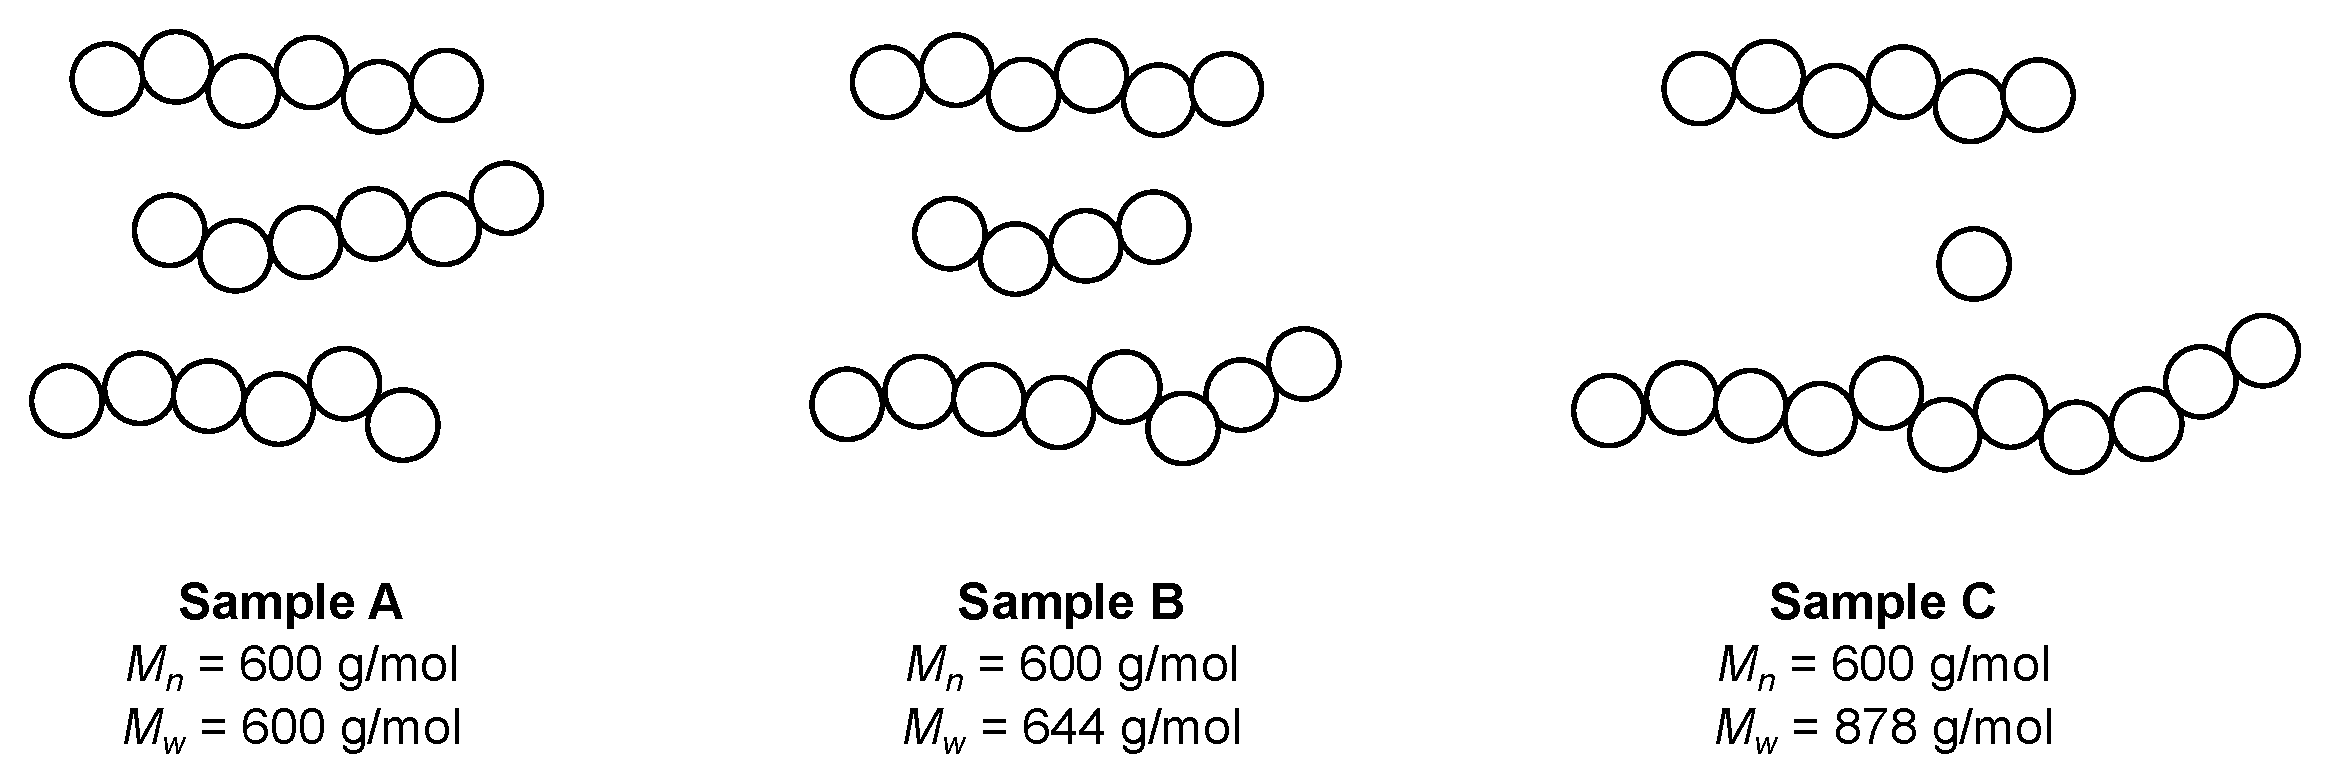
\includegraphics[width=0.9\textwidth]{\figpath/model2-samples}}

\end{model}
	
\begin{ctqs}

	\question Briefly describe your qualitative observations about how $M_n$ and $M_w$ change with the distribution of chain lengths in the samples shown in Model \ref{\labelbase:mdl:dispersity}:
	
		\begin{solution}[2in]{}
			In this model, the number-average molecular weight of all of the samples is the same.  However, as the differences in the lengths of chains within the sample become larger (e.g. as the distribution becomes broader), the weight-average molecular weight increases.
		\end{solution}
	
\end{ctqs}

\begin{infobox}

	The relationship between $M_n$ and $M_w$ can be summarized by a quantity called the \emph{dispersity}.  The dispersity of a polymer sample, denoted \PDItext, is defined as
	\begin{equation*}
		\PDImath = \frac{M_w}{M_n}
	\end{equation*}
	
\end{infobox}

\begin{ctqs}

	\question Calculate the dispersity of each of the polymer samples shown in Model \ref{\labelbase:mdl:dispersity}:
	
				\begin{center}
					\renewcommand{\arraystretch}{3}
					\begin{tabular}{|c|c|}
						\hline
						\textbf{Sample} & \hspace{2cm}\textbf{\PDItext}\hspace{2cm} \\\hline
						A     &       \answer{1}             \\\hline
						B     &       \answer{1.07}             \\\hline
						C     &       \answer{1.46}             \\\hline
					\end{tabular}
				\end{center}
				\vspace{10pt}
	
	\question Describe, in your own words, what it means when the dispersity is...
	
		\begin{enumerate}
			\item ... equal to 1:
			
				\begin{solution}[0.75in]{}
					When the dispersity is equal to one, all of the chains are exactly the same length.
				\end{solution}
			
			\item ... slightly greater than 1:
			
				\begin{solution}[0.75in]{}
					When the dispersity is slightly greater than one, the chains have similar lengths, but there is some variation from chain to chain.
				\end{solution}
			
			\item ... much greater than 1:
			
				\begin{solution}[1in]{}
					When the dispersity is much greater than one, the different chains in the samples have very different lengths.  There is a lot of variation in the chain lengths.
					
					Note for instructors: it may be worth commenting that while there are no distinct cutoffs, dispersities between 1 and 1.5 are generally considered relatively narrow, while dispersities above 2 are generally considered pretty broad.  Students may find this surprising (sample C already looks like it has a lot of variation), but some commercial polymerizations do produce dispersities in the range of 2-10, so it is all matter of perspective!
				\end{solution}
			
		\end{enumerate}
		
	\question Can the dispersity ever be less than one?  Briefly justify your answer in 1-2 complete sentences.
	
		\begin{solution}[2in]{}
			No. Because the weight-average molecular weight is always greater than or equal to the number-average molecular weight (see question \ref{\labelbase:ctq:MWvsMN}), 
			the dispersity will always be greater than or equal to one.
		\end{solution}
	
\end{ctqs}



\begin{exercises}

		\exercise The equations for $M_n$ and $M_w$ given in the activity are given in terms of $n_i$, the number of chains with degree of polymerization $i$, and $M_0$, the molecular weight of a single monomer.
		
		Show that each of the following are equivalent expressions for $M_n$ and $M_w$:
		
			\begin{enumerate}
				
				\item \begin{align*}
					M_n = \frac{\sum_i n_i M_i}{\sum_i n_i} && \text{and} &&  M_w = \frac{\sum_i n_i M_i^2}{\sum_i n_i M_i}
				\end{align*}
					where $n_i$ is the number of chains of length $i$ and $M_i$ is the molecular weight of each chain of length $i$.
					
					\begin{solution}{}
					
						On page \pageref{\labelbase:infobox:MnMw}, we are told that he number-average molecular weight is given by
	\begin{equation*}
		M_n = M_0 \frac{\sum_i n_i i}{\sum_i n_i}
	\end{equation*}
	while the weight-average molecular weight is given by
	\begin{equation*}
		M_w = M_0 \frac{\sum_i n_i i^2 }{\sum_i n_i i}
	\end{equation*}
	
	To rewrite these expressions in the requested form, we just need to recognize that the molecular weight of a chain of length $i$ is $M_i = M_0 i$.  Thus, rearranging,
	\begin{align*}
		M_n = M_0 \frac{\sum_i n_i i}{\sum_i n_i}
			= \frac{\sum_i  n_i M_0 i}{\sum_i n_i}
			= \frac{\sum_i  n_i M_i}{\sum_i n_i}
	\end{align*}
	and
	\begin{align*}
		M_w = M_0 \frac{\sum_i n_i i^2 }{\sum_i n_i i}
			= \frac{M_0^2}{M_0} \frac{\sum_i n_i i^2 }{\sum_i n_i i}
			= \frac{\sum_i n_i M_0^2 i^2 }{\sum_i n_i M_0 i}
			= \frac{\sum_i n_i M_i^2 }{\sum_i n_i M_i}
	\end{align*}
	as desired.
	
					\end{solution}
				
				\item  \begin{align*}
					M_n = \sum_i x_i M_i && \text{and} && M_w = \sum_i w_i M_i
				\end{align*}
					where $x_i$ is the \emph{mole fraction} of chains that have length $i$, and $w_i$ is the \emph{weight fraction} (fraction of the total mass) that comes from chains of length $i$.
					
					\begin{solution}{}
						To address this question, we need to realize that the mole fraction of chains that have length $i$ is
						\begin{equation*}
							x_i = \frac{\text{number of chains of length } i}{\text{total number of chains}} = \frac{n_i}{\sum_i n_i}
						\end{equation*}
						while the weight fraction is
						\begin{equation*}
							w_i = \frac{\text{weight of chains of length } i}{\text{total weight of chains}} = \frac{n_i M_i}{\sum_i n_i M_i}
						\end{equation*}
						(note that a single chain of length $i$ has mass $M_i$ so if there are $n_i$ chains of this length, then the weight of chains of length $i$ is $n_i M_i$).
						
						Using these to rearrange the expressions for $M_n$ and $M_w$ from the previous part, we find
	\begin{align*}
		M_n = \frac{\sum_i  n_i M_i}{\sum_j n_i}
			= \sum_i \left(\frac{n_i}{\sum_j n_j}\right) M_i
			= \sum_i x_i M_i
	\end{align*}
	\begin{align*}
		M_w = \frac{\sum_i n_i M_i^2 }{\sum_j n_i M_i}
			= \sum_i \left(\frac{n_i M_i}{\sum_j n_j M_j}\right) M_i
			= \sum_i w_i M_i
	\end{align*}
	as desired.  (Note that we have changed the summation index in the denominator to $j$ to avoid confusion in the nested sums.)
						
					\end{solution}
				
			\end{enumerate}
			
		\exercise Calculate the number-average and weight-average molecular weights of...
		
			\begin{enumerate}
			
				\item ... a sample that contains 1 mole each of hexane (\ce{C6H14}) and dodecane (\ce{C12H26}).
					
					\begin{solution}{}
						For this problem, we should recognize that we are given the quantities of each component in terms of the number of moles, so we should use the expressions given in terms of $n_i$.
						
						As such, the number-average molecular weight of this sample is
						\begin{align*}
							M_n &= \frac{(1\text{ mol})(86.2\text{ g/mol})+(1\text{ mol})(170.3\text{ g/mol})}{2\text{ mol}} \\
								&= 128.3\text{ g/mol}\\
								&\sim 1.3\times 10^2\text{ g/mol}
						\end{align*}
						and the weight-average molecular weight is
						\begin{align*}
							M_w &= \frac{(1\text{ mol})(86.2\text{ g/mol})^2+(1\text{ mol})(170.3\text{ g/mol})^2}{(1\text{ mol})(86.2\text{ g/mol})+(1\text{ mol})(170.3\text{ g/mol})} \\
								&= 142.0\text{ g/mol}\\
								&\sim 1.4\times 10^2\text{ g/mol}
						\end{align*}
					\end{solution}
				
				\item ... a sample that contains 1 gram each of hexane (\ce{C6H14}) and dodecane (\ce{C12H26}).
					
					\begin{solution}{}
						For this problem, we should recognize that we are given the quantities of each component in terms of total mass.  We can use the same equations as before, but we need to calculate the number of moles of each component first:
						
						\begin{itemize}
							\item hexane: (1 g)/(86.2 g/mol) = 0.01160 mol
							\item dodecane: (1 g)/(170.3 g/mol) = 0.00587 mol
						\end{itemize}
						
						As such, the number-average molecular weight of this sample is
						\begin{align*}
							M_n &= \frac{(0.0116\text{ mol})(86.2\text{ g/mol})+(0.0059\text{ mol})(170.3\text{ g/mol})}{(0.0116+0.0059)\text{ mol}} \\
								&= 114.5\text{ g/mol}\\
								&\sim 1.1\times 10^2\text{ g/mol}
						\end{align*}
						and the weight-average molecular weight is
						\begin{align*}
							M_w &= \frac{(0.0116\text{ mol})(86.2\text{ g/mol})^2+(0.0059\text{ mol})(170.3\text{ g/mol})^2}{(0.0116\text{ mol})(86.2\text{ g/mol})+(0.0059\text{ mol})(170.3\text{ g/mol})} \\
								&= 127.9\text{ g/mol}\\
								&\sim 1.3\times 10^2\text{ g/mol}
						\end{align*}
						
						Note that the averages in part (b) are both lower than the averages in part (a) because the sample contains proportionately more molecules of the lower-molecular-weight hexane.
					\end{solution}
				
			\end{enumerate}
			
		\exercise The standard deviation in the molecular weights of a sample is related to the dispersity by
		
			\begin{align*}
					\sigma = M_n\sqrt{\PDImath - 1}
			\end{align*}
			
			\begin{enumerate}
				\item What is the standard deviation in the molecular weight for a sample with $M_n=25$~kg/mol and $\PDImath=1.25$?
					
					\begin{solution}{}
						\begin{equation*}
							\sigma = 25\text{ kg/mol}\sqrt{1.25-1} = 12.5\text{ g/mol} \approx 13\text{ g/mol}
						\end{equation*}
						
						Students may find this surprising - that is already a pretty big standard deviation, even for a dispersity that's kind of on the edge of what we would consider a ``narrow'' distribution!
					\end{solution}
				
				\item How small would the dispersity need to be for the standard deviation to be less than 10\% of $M_n$?
					
					\begin{solution}
					This question is essentially asking, when is $\sigma/M_n < 0.1$?  To address this, we just need to rearrange the given equation a bit:
					\begin{equation*}
						\PDImath = \left(\frac{\sigma}{M_n}\right)^2 + 1 = 0.1^2 + 1 = 1.01
					\end{equation*}
					Thus, the standard deviation in the molecular weights would be less than 10\% of $M_n$ when $\PDImath<1.01$.
					\end{solution}
					
			\end{enumerate}
			
\end{exercises}
	
\end{activity}
		%%%%%%%%%%%%%%%%%%%%%%%%%%%%%%%%%%%%%%%%%
%
% (c) 2022 by Jennifer Laaser
%
% This work is licensed under the Creative Commons Attribution-NonCommercial-ShareAlike 4.0 International License. To view a copy of this license, visit http://creativecommons.org/licenses/by-nc-sa/4.0/ or send a letter to Creative Commons, PO Box 1866, Mountain View, CA 94042, USA.
%
% The current source for these materials is accessible on Github: https://github.com/jlaaser/pogil-polymers
%
%%%%%%%%%%%%%%%%%%%%%%%%%%%%%%%%%%%%%%%%%

\renewcommand{\figpath}{content/intro/measuring-MW/figs}
\renewcommand{\labelbase}{measuring-MW}

\begin{activity}{Measuring Molecular Weight}
\label{\labelbase}

\begin{instructornotes}

	This activity introduces students to key concepts related to methods used to measure the molecular weights and molecular weight distributions of polymers.
	
	After completing this activity, students will be able to:
			\begin{enumerate}
				\item Use end-group analysis via NMR and UV-Vis to calculate the number-average molecular weight of a polymer
				\item Qualitatively interpret the relative molecular weights and dispersities of polymers measured by SEC
				\item Interpret MALDI spectra in terms of the repeat unit mass and frequency of chain lengths, and calculate molecular weights and dispersities of polymer samples from MALDI data
			\end{enumerate}
			
	\subsection*{Activity summary:}
	\begin{itemize}
		\item \textbf{Activity type:} Learning Cycle
		\item \textbf{Content goals:} Measuring molecular weights
		\item \textbf{Process goals:} %https://pogil.org/uploads/attachments/cj54b5yts006cklx4hh758htf-process-skills-official-pogil-list-2015-original.pdf
			\begin{itemize}
				\item Interpreting graphs and numeric data
				\item Written and oral communication of reasoning
			\end{itemize}
		\item \textbf{Duration:} TBD
		\item \textbf{Instructor preparation required:} none beyond knowledge of relevant content
		\item \textbf{Related textbook chapters:}
			\begin{itemize}
				\item \emph{Polymer Chemistry} (Hiemenz \& Lodge): section 1.8
			\end{itemize}
		%\item \textbf{Facilitation notes:}
		%	\begin{itemize}
		%		\item \dots
		%	\end{itemize}
	\end{itemize}
	
\end{instructornotes}




\begin{model}[End Group Analysis]
\label{\labelbase:mdl:endgrpanalysis}

	\dots

\end{model}


\begin{ctqs}

	\question \dots
	
\end{ctqs}

\begin{infobox}

	\dots

\end{infobox}

\begin{ctqs}
		
	\question \dots
	
\end{ctqs}



\begin{model}[Size-Exclusion Chromatography]
\label{\labelbase:mdl:SEC}
	
	\dots

\end{model}

\begin{ctqs}

	\question \dots
	
\end{ctqs}



\begin{model}[MALDI Mass Spectrometry]
	\label{\labelbase:mdl:MALDI}

	\dots

\end{model}

\begin{ctqs}

	\question \dots
		
\end{ctqs}


\begin{exercises}

	\exercise \dots
	
\end{exercises}


	
\end{activity}

\part{Polymer Chemistry}

	\chapter{Fundamentals of Polymer Chemistry}
		%%%%%%%%%%%%%%%%%%%%%%%%%%%%%%%%%%%%%%%%%
%
% (c) 2018 by Jennifer Laaser
%
% This work is licensed under the Creative Commons Attribution-NonCommercial-ShareAlike 4.0 International License. To view a copy of this license, visit http://creativecommons.org/licenses/by-nc-sa/4.0/ or send a letter to Creative Commons, PO Box 1866, Mountain View, CA 94042, USA.
%
% The current source for these materials is accessible on Github: https://github.com/jlaaser/pogil-polymers
%
%%%%%%%%%%%%%%%%%%%%%%%%%%%%%%%%%%%%%%%%%

\renewcommand{\figpath}{content/intro/chain-and-step/figs}
\renewcommand{\labelbase}{chain-and-step}

\begin{activity}{Introduction to Polymerization Mechanisms}
\begin{instructornotes}

	This activity introduces students to key concepts related to the chain-growth and step-growth polymerization mechanisms.
	
	After completing this activity, students will be able to:
			\begin{enumerate}
				\item Compare and contrast the mechanisms of chain- and step-growth polymerizations
				\item Compare and contrast the molecular weight distributions that arise from chain- and step-growth polymerizations
				\item Compare and contrast the kinetics of chain- and step-growth polymerizations
			\end{enumerate}
			
	This activity also provides students with additional practice in calculating $M_n$, $M_w$, and $\PDImath$ from a given distribution of chain lengths.
			
	\subsection*{Activity summary:}
	\begin{itemize}
		\item \textbf{Activity type:} Learning Cycle
		\item \textbf{Content goals:} Basic polymerization mechanisms
		\item \textbf{Process goals:} %https://pogil.org/uploads/attachments/cj54b5yts006cklx4hh758htf-process-skills-official-pogil-list-2015-original.pdf
			written communication, critical thinking, information processing
		\item \textbf{Duration:} 75 minutes, including discussion 
		
			\emph{Note: the simulations in Models 1 and 2 (and appropriate clean-up) can generally be completed in about 20 minutes if students skip the intermediate questions.  As long as they complete the tables in CTQs 1 and 7, the remainder of the analysis can be finished in a later class period if necessary.}
			
		\item \textbf{Instructor preparation required:} 
		
			This activity is designed for use with ``pop beads'' sold as a children's toy (often for jewelry making).  Large bags of assorted colors can be purchased from vendors such as Amazon and Walmart at low cost.  Prior to class, the beads should be sorted by color, and divided up into bags of approx. 100 beads per color.
		
			At the beginning of the activity, each group of 4 students should be supplied with two bags of beads in the same color (for use in the chain-growth polymerization in Model 1) and two bags of beads in different colors (for use in the step-growth polymerization in Model 2).  The instructor should reserve one color of beads as the ``initiator beads'' to be handed out at the beginning of Model 1.
		
			At the end of the activity, it is helpful to ask the students to ``de-polymerize'' their chains and sort the beads by color back into their original bags to minimize instructor setup for the next time.
			
			\emph{Note: 100 beads per bag will result in simulations that take 4-5 minutes each for groups of four students.  If student groups are larger or smaller, increase or decrease the number of beads accordingly.}
		
		\item \textbf{Related textbook chapters:}
			\begin{itemize}
				\item \emph{Polymer Chemistry} (Hiemenz \& Lodge): sections 1.4.1, 2.2, and 3.2
			\end{itemize}
	\end{itemize}

\end{instructornotes}

\newcommand{\timeallowed}{3 minutes}

\begin{model}[Chain-Growth Polymerizations]
\label{\labelbase:mdl:chaingrowth}

	In one important type of polymerization, monomers cannot react with each other; they can only become part of a polymer chain if they react with the ``active'' end of an existing chain.
	
	Simulate this type of polymerization by doing the following:
	\begin{enumerate}
		\item Combine two bags of beads of the same color in your group's bin, and place it where everyone can reach it.
		\item Start a timer to keep track of the amount of time needed for the simulation.
		\item As soon as the timer is started, go to your instructor and obtain a special ``initiator'' bead, then return to your desk. \emph{Note: each person in the group needs their own initiator bead!}
		\item Pick up beads one at a time from your group's bin, and add them to the chain according to the following rules:
			\begin{itemize}
				\item Attach the first bead directly to the initiator bead.
				\item All subsequent beads must be added to the growing end of the chain, \emph{not} to the initiator end.
			\end{itemize}
		\item Keep adding beads until all of the beads are incorporated into the growing chains.  Record the time elapsed here: \rule{1in}{0.15mm}
	\end{enumerate}
	
	Use the chains generated in this simulation to answer this Model's CTQs, below.

\end{model}

\vspace{0.05in}
\begin{ctqs}

	\question Count the number of beads in each chain (excluding the initiator bead), and fill in the following table: \label{\labelbase:ctq:numbeadschain}
		
		\begin{center}
		\renewcommand{\arraystretch}{2.2}
			\begin{tabular}{|c|c|c|c|}
				\hline
				\textbf{Chain Length ($i$)} & \textbf{Number of Chains of Length $i$ ($n_i$)} & \hspace{0.75in} & \hspace{0.75in} \\\hline
				\answer{46} &\answer{1}&&\\\hline
				\answer{49}&\answer{2}&&\\\hline
				\answer{51}&\answer{1}&&\\\hline
				&&&\\\hline
				&\answer{(sample data - student answers will vary)}&&\\\hline
			\end{tabular}
		\end{center}
		
		\emph{(Note: the two empty columns do not need to be filled in yet - you will get to them in CTQ \ref{\labelbase:ctq:Dchain}.)}
		
	\question On the following axes, sketch a graph of $n_i$ vs $i$ and briefly describe its shape. \label{\labelbase:ctq:MWDchain}
	
		\emph{Note: for any values of $i$ for which you didn't have any chains of that length, make sure you indicate that $n_i$ is zero!}
	
		\begin{solution}[2.5in]\studentdisplay{
			\centerline{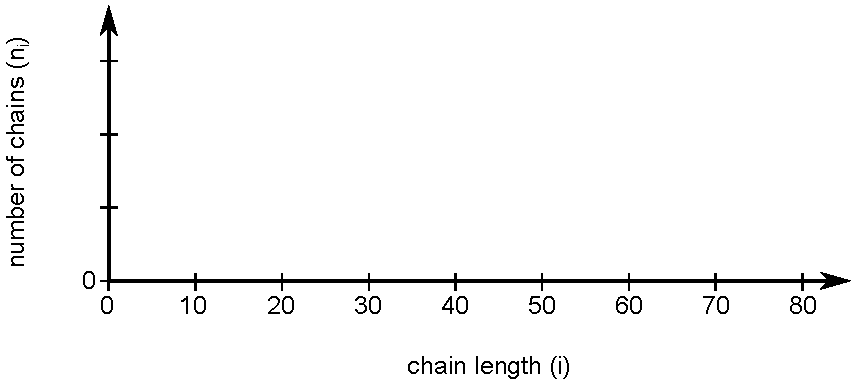
\includegraphics[width=5in]{\figpath/MWD-plots-blank}}
		}\instructordisplay{
			Example plot:
			
			\centerline{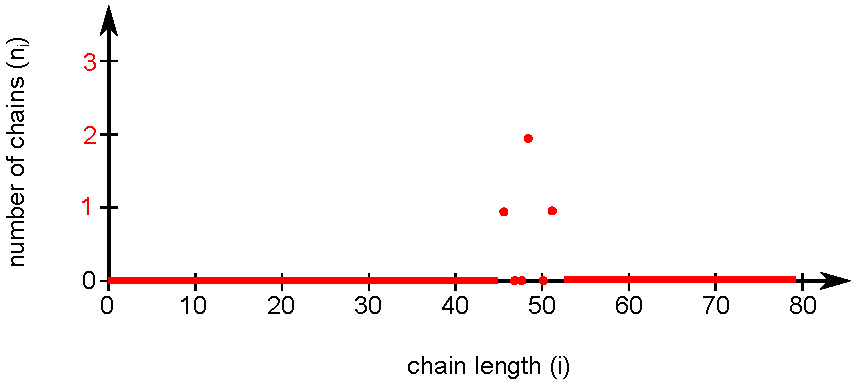
\includegraphics[width=5in]{\figpath/MWD-plots-chaingrowth-answer}}
		}\end{solution}
	
	\question Calculate $M_n$, $M_w$, and \PDItext\ for this polymerization.  Assume that each bead represents a monomer with a molecular weight of 100~g/mol. \label{\labelbase:ctq:Dchain}
	
		\emph{Hint: you may find it useful use the extra columns in CTQ \ref{\labelbase:ctq:numbeadschain} to do some of the intermediate steps in the calculation, as we did in Activity 1.\ref{M-and-D}.}
	
		\begin{solution}[2.5in]\instructordisplay{
		
			Students should fill in the two blank columns in CTQ 1 with $n_i i$ and $n_i i^2$.  They can then calculate the sum of each column and use these sums to obtain $M_n$, $M_w$, and $\PDImath$ as in Activity 3.
			
			For the sample data shown in CTQ 1,
			
			\begin{equation*}
				M_n = M_0\frac{\sum_i i n_i}{\sum_i n_i} = (100\text{ g/mol})\frac{46\cdot 1 + 49\cdot 2 + 51\cdot 1}{1+2+1} = 4875\text{ g/mol}
			\end{equation*}
			\begin{equation*}
				M_w = M_0\frac{\sum_i i^2 n_i}{\sum_i i n_i} = (100\text{ g/mol})\frac{46^2\cdot 1 + 49^2\cdot 2 + 51^2\cdot 1}{46\cdot 1 + 49\cdot 2 + 51\cdot 1} = 4882\text{ g/mol}
			\end{equation*}
			\begin{equation*}
				\PDImath = \frac{M_w}{M_n} = \frac{4875\text{ g/mol}}{4882\text{ g/mol}} = 1.001
			\end{equation*}
		}\end{solution}
	
	\question Based on your graph from CTQ \ref{\labelbase:ctq:MWDchain}, and the dispersity you calculated in CTQ \ref{\labelbase:ctq:Dchain}, would you characterize the molecular weight distribution generated by this polymerization as ``narrow'' or ``broad''?  %Briefly explain your reasoning.
	
		\begin{solution}[1in]
			The molecular weight distribution is narrow because there is not much variation in the chain lengths, and the dispersity is close to 1.
		\end{solution}
	
	\question If each member of your group had picked up their initiator bead at a different time, how would the molecular weight distribution and dispersity have changed?  Explain your group's reasoning in 2-3 complete sentences.
	
		\begin{solution}[1.9in]
			If each group member had picked up their initiator beads at different times, the molecular weight distribution would have been broader, and the dispersity would have been larger.  This is because the students who started first would have had more time to add beads to their chains and would have ended up with longer chains, while the students who started later would not have had as much time to add beads to their chains and would have ended up with shorter chains.
		\end{solution}
	
	\question If everyone in your group had picked up their initiator bead at the same time, but each person added beads at a different rate, how would the molecular weight distribution and dispersity have changed?  Explain your group's reasoning in 2-3 complete sentences.
	
		\begin{solution}[1.9in]
			If each group member had added beads at a different rate, the molecular weight distribution would have been broader, and the dispersity would have been larger.  This is because the students who added beads faster would end up with longer chains than in the current simulation, while students who added beads slower would end up with shorter chains.
		\end{solution}
		
\end{ctqs}

\begin{model}[Step-Growth Polymerizations]
\label{\labelbase:mdl:stepgrowth}

	Another type of polymerization uses monomers that each have two or more reactive sites.  Every molecule (monomer or polymer) may react with every other molecule (monomer or polymer) as long as they have complimentary reactive groups on their ends that are able to form a bond.
	
	Simulate this type of polymerization by doing the following:
	\begin{enumerate}
		\item Combine two bags of beads of different colors in your group's bin.  Remove any beads left over from the previous simulation if you have not done so already.
		\item Set a timer for however much time was required for the polymerization in Model \ref{\labelbase:mdl:chaingrowth}.
		\item Start the timer!
		\item Start the polymerization by having each person pick up two beads \emph{of different colors}, connect them, and drop them back into the bin.
		\item Continue the polymerization by doing the following:
			\begin{itemize}
				\item Pick up two pieces (single beads, or strings of beads - try to choose as randomly as possible!) from the bin.
				\item If it is possible to connect the two pieces you picked up by connecting beads \emph{of different colors}, connect the two pieces and return them to the bin.
				\item Otherwise, return both pieces to the bin and try again.
			\end{itemize}
		\item Continue connecting beads until your timer goes off.
	\end{enumerate}
	
	Use the chains generated in this simulation to answer this Model's CTQs, below.

\end{model}
	
\begin{ctqs}

	\question Count the number of beads in each chain, and fill in the following table.  Count unreacted monomer beads as chains of length 1. \label{\labelbase:ctq:numbeadsstep}
		
		\begin{center}
		\renewcommand{\arraystretch}{2}
			\begin{tabular}{|c|c|c|c|}
				\hline
				\textbf{Chain Length ($i$)} & \textbf{Number of Chains of Length $i$  ($n_i$)} & \hspace{0.75in} & \hspace{0.75in} \\\hline
				\answer{1}&\answer{58}&&\\\hline
				\answer{2}&\answer{45}&&\\\hline
				\answer{3}&\answer{29}&&\\\hline
				\answer{4}&\answer{24}&&\\\hline
				\answer{5}&\answer{12}&&\\\hline
				\answer{6}&\answer{13}&&\\\hline
				\answer{8}&\answer{3}&&\\\hline
				\answer{9}&\answer{5}&&\\\hline
				\answer{10}&\answer{2}&&\\\hline
				\answer{15}&\answer{1}&&\\\hline
				&&&\\\hline
				&&&\\\hline
				&\answer{(sample data - student answers will vary)}&&\\\hline
				&&&\\\hline
				&&&\\\hline
			\end{tabular}
		\end{center}
		
	\question Sketch a graph of $n_i$ vs $i$ and briefly describe its shape. \label{\labelbase:ctq:MWDstep}
	
		\begin{solution}[3in]\studentdisplay{
			\centerline{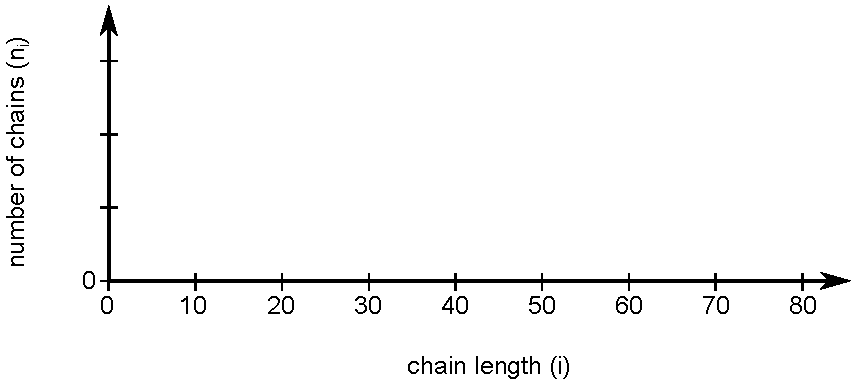
\includegraphics[width=5in]{\figpath/MWD-plots-blank}}
		}\instructordisplay{
			Example plot:
			
			\centerline{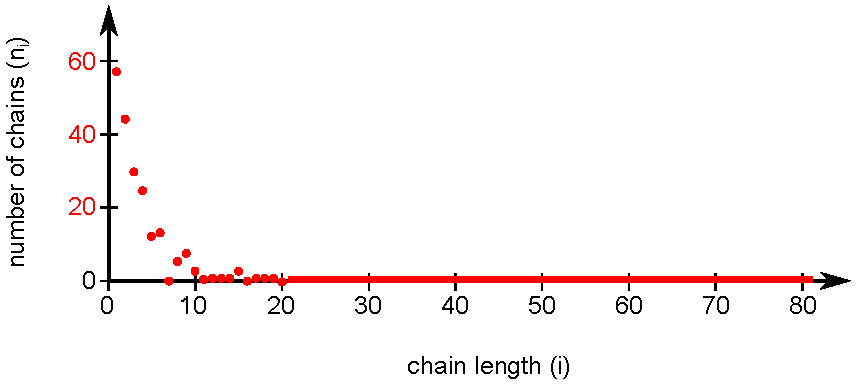
\includegraphics[width=5in]{\figpath/MWD-plots-stepgrowth-answer}}
		}
		\end{solution}
	
	\question Calculate $M_n$, $M_w$, and \PDItext\ for this polymerization.  Assume that each bead represents a monomer with a molecular weight of 100~g/mol. \label{\labelbase:ctq:Dstep}
	
		\begin{solution}[3in]\instructordisplay{
			This calculation follows the same approach as in CTQ \ref{\labelbase:ctq:Dchain}.
			
			For the sample data shown above,
			\begin{align*}
				\sum_i n_i = 192 && \sum_i i n_i = 573 && \sum_i i^2 n_i = 2673
			\end{align*}
			so
			\begin{align*}
				M_n = 298\text{ g/mol} && M_w = 466\text{ g/mol} && \PDImath = 1.56
			\end{align*}
			
			(Note that the dispersity is somewhat lower than the limiting value of 2 for step-growth polymerizations because the extent of reaction is relatively low.)
		}\end{solution}
	
	\question Based on your graph from CTQ \ref{\labelbase:ctq:MWDstep}, and the dispersity you calculated in CTQ \ref{\labelbase:ctq:Dstep}, would you characterize the molecular weight distribution generated by this polymerization as ``narrow'' or ``broad''?  %Briefly explain your reasoning.
	
		\begin{solution}[1in]\instructordisplay{
			This molecular weight distribution is not extremely broad (the dispersity is not larger than 2), but it is also not nearly as narrow as the molecular weight distribution generated in Model \ref{\labelbase:mdl:chaingrowth}.  A dispersity of 1.5 is right on the edge of what we typically consider narrow.
		}\end{solution}
	
	\question Suppose you had kept going with the simulation until no more  connections could be made.  What would be the result?  Explain your group's reasoning in 2-3 complete sentences.
	
		\begin{solution}[1.75in]
			Eventually, all of the beads would have ended up connected into a single long chain.
		\end{solution}
	
	\question If there had been significantly more beads of one color than the other, how would the final distributions of chains be different?  Explain your group's reasoning in 2-3 complete sentences.
	
		\begin{solution}[1.75in]
			If there were significantly more beads of one color than the other, the final sample would contain many shorter chains, each capped by the color of bead present in excess.  This is because once all of the chains end in the color present in excess, no further reactions can take place, so the chains stop growing.
		\end{solution}
	
\end{ctqs}

\begin{infobox}
	The type of polymerization you simulated in Model  \ref{\labelbase:mdl:chaingrowth} is called a \emph{chain-growth} polymerization, while the type of polymerization you simulated in Model  \ref{\labelbase:mdl:stepgrowth} is called a \emph{step-growth} polymerization.
	
	All of the polymerization methods we discuss in class will fall into one of these two categories, and it is useful to recognize the advantages and disadvantages of each approach.
\end{infobox}

\begin{ctqs}
	\question Which polymerization mechanism (chain-growth or step-growth) gave longer polymers in the time allowed for the simulation?
	
		\begin{solution}[1in]
			The chain-growth polymerization gave longer polymers in the time allowed for the simulation.
		\end{solution}
	
	\question Which method would give the longest polymers if there were an infinite amount of time?  Explain your group's reasoning in 1-2 complete sentences.
	
		\begin{solution}[1.75in]
			If there were an infinite amount of time, the step-growth polymerization would give longer chains because the monomers could (if there were equal numbers of beads of each color) theoretically all combine into a single long chain, while the monomers for the chain-growth polymerization are necessarily divided up into a number of chains equal to the number of initiator beads.
		\end{solution}
	
	\question Which polymerization mechanism gave a larger dispersity?  In 2-3 complete sentences, explain why your group thinks this happened.
	
		\begin{solution}[1.75in]
			The step-growth polymerization gave a larger dispersity.  This is because the polymerization process was much more random, and so there ended up being a broader distribution of chain lengths.
		\end{solution}
	
	\question If you needed to make a batch of 700~kg/mol polyethylene, which type of polymerization would you choose?  Explain your group's choice in 1-2 complete sentences.
	
		\begin{solution}[1.75in]
			A chain-growth polymerization would be most suitable.  Although step-growth polymerizations can theoretically reach higher molecular weights, they take a VERY long time to get there, so it would likely be impractical to prepare a 700~kg/mol polymer using this method.
			
			(Note: once students learn about the chemistries for chain-growth and step-growth polymerization, they will hopefully also recognize that polyethylene can't be prepared by step-growth polymerization, either, because the ethylene monomers can't react directly with each other.)
		\end{solution}
	
\end{ctqs}

\clearpage
\begin{exercises}

		\exercise In a brief paragraph, describe the key differences between the chain-growth and step-growth polymerization mechanisms.
		
		\begin{solution}\instructordisplay{
			In chain-growth polymerizations, the monomers can only react with the ``active'' end of a polymer chain, while in a step-growth polymerization, they can react directly with each other or with other chains.  The kinetics are also very different: chain growth polymerizations also generate longer chains much more quickly than step-growth polymerizations do.  Finally, the molecular weight distributions are different. At least for the chain-growth process demonstrated in this activity, the molecular weight distribution was sharply peaked at a relatively long chain length, while for the step-growth polymerization the molecular weight distribution was much broader and centered around shorter chain lengths (and, in fact, the most common species in the mixture was unreacted monomer!).
		}\end{solution}
		
		\exercise Summarize the key conditions necessary for a chain-growth polymerization to achieve a narrow molecular weight distribution.
		
			\begin{solution}\instructordisplay{
				As demonstrated in this activity, two of the key conditions necessary for a chain-growth polymerization to achieve a narrow molecular weight distribution are:
				\begin{itemize}
					\item All chains must start growing at the same time
					\item All chains must grow at the same rate
				\end{itemize}
				
				Although not demonstrated in this activity, two additional requirements apply:
				\begin{itemize}
					\item The polymerization must proceed in the absence of irreversible termination reactions
					\item The polymerization must proceed in the absence of irreversible chain-transfer reactions
				\end{itemize}
				These requirements will be covered in more detail later in this course.
			}\end{solution}
			
\end{exercises}
	
\end{activity}

	\chapter{Step-Growth Polymerizations}
		%%%%%%%%%%%%%%%%%%%%%%%%%%%%%%%%%%%%%%%%%
%
% (c) 2019 by Jennifer Laaser
%
% This work is licensed under the Creative Commons Attribution-NonCommercial-ShareAlike 4.0 International License. To view a copy of this license, visit http://creativecommons.org/licenses/by-nc-sa/4.0/ or send a letter to Creative Commons, PO Box 1866, Mountain View, CA 94042, USA.
%
% The current source for these materials is accessible on Github: https://github.com/jlaaser/pogil-polymers
%
%%%%%%%%%%%%%%%%%%%%%%%%%%%%%%%%%%%%%%%%%

\renewcommand{\figpath}{content/polymchem/stepgrowth/stepgrowth-chemistries/figs}
\renewcommand{\labelbase}{stepgrowth-chem}

\begin{activity}{Chemistries of Step-Growth Polymerizations}

\begin{instructornotes}

	This activity introduces students to key chemistries used for step-growth polymerizations.
	
	After completing this activity, students will be able to:
			\begin{enumerate}
				\item Identify major classes of polymers produced by step-growth polymerization
				\item Determine the polymer produced by a given monomer or monomer pair, and determine the monomer(s) necessary to produce a target polymer
				\item Determine whether or not a reaction qualifies as a condensation polymerization, and if so, identify the small molecule released
			\end{enumerate}
	
			
	\subsection*{Activity summary:}
	\begin{itemize}
		\item \textbf{Activity type:} Learning Cycle
		\item \textbf{Content goals:} Chemistries of step-growth polymerizations
		\item \textbf{Process goals:} %https://pogil.org/uploads/attachments/cj54b5yts006cklx4hh758htf-process-skills-official-pogil-list-2015-original.pdf
			written communication, critical thinking, information processing
		\item \textbf{Duration:} approx. 45 minutes
		\item \textbf{Instructor preparation required:} none beyond knowledge of relevant content
		\item \textbf{Related textbook chapters:}
			\begin{itemize}
				\item \emph{Polymer Chemistry} (Hiemenz \& Lodge): Table 1.2 and sections 2.2.1, 2.5, and 2.6
			\end{itemize}
	\end{itemize}

\end{instructornotes}

	%\textbf{Focus question:} Put a central question for the students to consider through this exercise here.

\begin{model}[Synthesis of a Polyester]
\label{\labelbase:mdl:polyester}

	Esterification reactions are a common type of reaction used to produce polymers by step-growth polymerization.
	In a typical esterification reaction, an alcohol and a carboxylic acid react to form an ester bond:
	
	\centerline{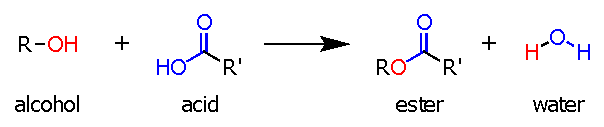
\includegraphics[width=0.7\textwidth]{\figpath/model1_ester-general.pdf}}
	
	One example of a polymerization reaction using this chemistry is the synthesis of poly(6-hydroxycaproic acid) from 6-hydroxycaproic acid monomers:
	
	\centerline{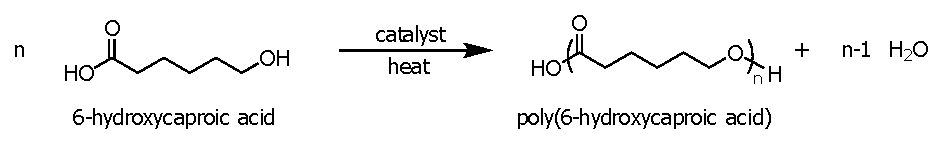
\includegraphics[width=0.9\textwidth]{\figpath/model1_P6HCA.pdf}}

\end{model}


\begin{ctqs}

	\question Consider the 6-hydroxycaproic acid monomer shown in Model \ref{\labelbase:mdl:polyester}: \label{\labelbase:ctq:label-6hcpa}
	
		\begin{enumerate}
			\item As drawn, what type of functional group is on the \emph{left} side of the monomer?
			
				\begin{solution}[1in]
					carboxylic acid (``acid'' is also fine)
				\end{solution}
			
			\item As drawn, what type of functional group is on the \emph{right} side of the monomer?
			
				\begin{solution}[1in]
					alcohol (or hydroxyl)
				\end{solution}
		\end{enumerate}
		
\end{ctqs}

\begin{infobox}

	When a monomer used in a step-growth polymerization has different reactive functional groups on each end, it is called an ``AB-type'' monomer.
	
	When a monomer used in a step-growth polymerization has the same reactive functional group on each end, it is called an ``AA-type'' or ``BB-type'' monomer.

\end{infobox}

\begin{ctqs}
		
		\question Would you classify the poly(6-hydroxycaproic acid) monomer used in this synthesis as an AA-type monomer or an AB-type monomer?  Briefly explain your answer in 1-2 complete sentences.
			
				\begin{solution}[1.75in]
					This is an AB-type monomer, because it has two different reactive functional groups in the same monomer.
				\end{solution}
		
		\question The synthesis of a short 6-hydroxycaproic acid oligomer from three monomers is shown explicitly, below: \label{\labelbase:ctq:6hcpa-oligomer}
	
\vspace{0.25in}	\centerline{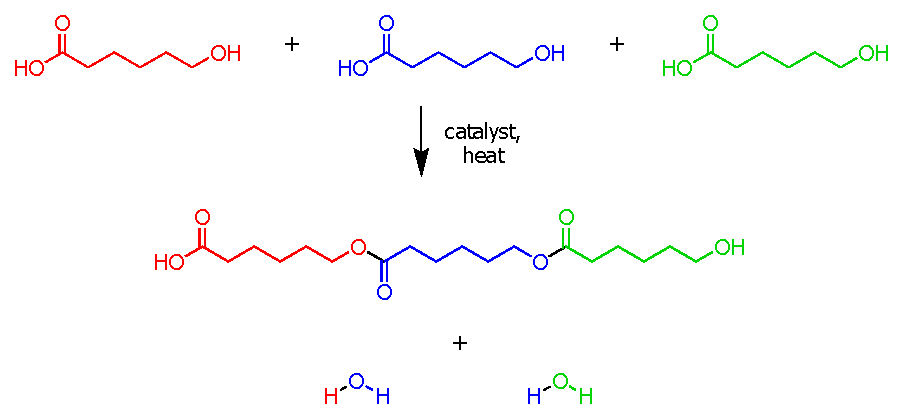
\includegraphics[width=0.9\textwidth]{\figpath/model1_3oligomer-explicit.pdf}}
The molecules are shaded and color-coded so that you can see which atoms in the oligomer came from which monomer.
		
		\begin{enumerate}
		
			\item What type of bonds connect the different monomers in the polymer backbone?
			
				\begin{solution}[1.5in]
					The monomers are connected by ester bonds.
				\end{solution}
		
			\item Explain, in one or two complete sentences, why you think we classify this polymer as a ``polyester'':
			
				\begin{solution}[2in]\instructordisplay{
					We call this polymer a ``polyester'' because it has ester groups in the polymer backbone.
					
					Note: the fact that they are in the backbone is important; if the ester groups are only in the sidechains, the polymer is \emph{not} a polyester - students will address this point in CTQ \ref{\labelbase:ctq:PMA}.
				}\end{solution}
	
			\item When we write the structure of this oligomer as
	
	\centerline{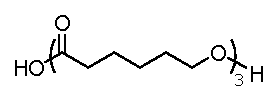
\includegraphics[width=0.25\textwidth]{\figpath/model1_3oligomer-shorthand.pdf}}
	\vspace{-3pt}
	how many different monomer molecules contribute to each repeat unit in the polymer chain?
			
				\begin{solution}[1in]
					one
				\end{solution}
		
			\item Explain, in one or two complete sentences, why we generally abbreviate the product of this reaction as
	
	\centerline{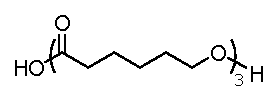
\includegraphics[width=0.25\textwidth]{\figpath/model1_3oligomer-shorthand.pdf}}
	
	rather than as
	
	\centerline{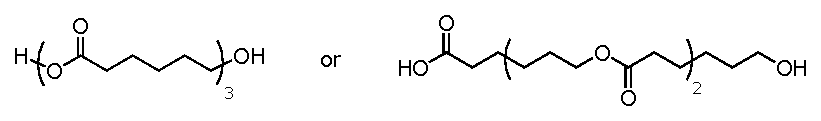
\includegraphics[width=0.7\textwidth]{\figpath/model1_incorrect-shorthand.pdf}}
			
				\begin{solution}[2in]
					We use the first notation because all of the atoms in a single repeat unit come from the same monomer (if you draw these parentheses on the color-coded molecules at the beginning of the question, each pair of parentheses will only have one color of atoms in it).  This is not true for the second and third options.
				\end{solution}
			
		\end{enumerate}
	
	\question Consider the following polymer:\label{\labelbase:ctq:PMA}
	
	\centerline{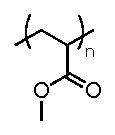
\includegraphics[width=0.1\textwidth]{\figpath/model1_PMA.pdf}}
	
		\begin{enumerate}
				
			\item Does this polymer have ester bonds in the polymer backbone?
			
				\begin{solution}[0.75in]
					No (they are only in the sidechains).
				\end{solution}
		
			\item Would you be able to produce this polymer by esterification reactions of small molecules?  Why or why not?
			
				\begin{solution}[2in]
					No.  This polymer (poly(methyl acrylate)) contains ester bonds, but they are only in the sidechains, not the backbone.  But when we produce a polymer from esterification reactions of small molecules, the ester bonds end up in the polymer backbone.
					
					Put another way, the backbone in this polymer only contains carbon-carbon bonds, which cannot be formed by esterification reactions.
				\end{solution}
			
			\item Based on your answers to the previous two questions, would you classify this polymer as a polyester?  Why or why not?
			
				\begin{solution}[2in]
					No, this is not a polyester because it does not contain ester bonds in the polymer backbone, and cannot be produced by esterification of small molecules.
				\end{solution}
			
		\end{enumerate}
		
\end{ctqs}
	

\clearpage
\begin{model}[Synthesis of a Polyamide]

Amidation reactions are another type of reaction used to produce polymers by step-growth polymerizations.
For example, acid chlorides can be reacted with primary amines to form an amide bond:
	
	\centerline{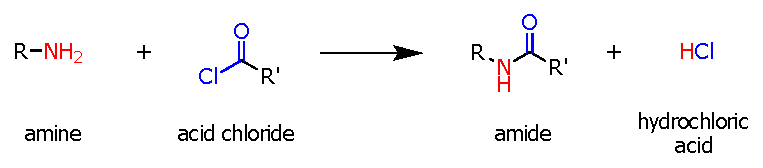
\includegraphics[width=0.7\textwidth]{\figpath/model2_amide-general.pdf}}

Commercially, this reaction is used to produce Nomex, a heat-resistant polymer used in oven mitts and firefighters' protective clothing, among other applications.
A reaction scheme for the synthesis of Nomex is shown below:
	
	\centerline{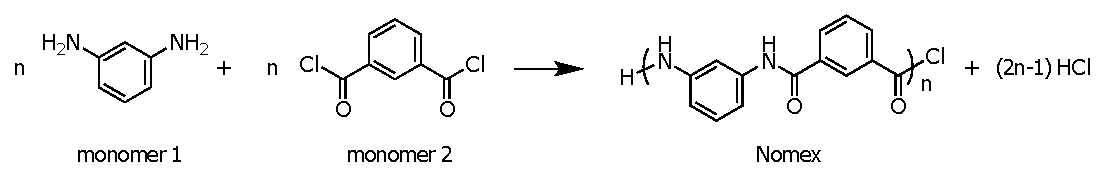
\includegraphics[width=0.9\textwidth]{\figpath/model2_Nomex.pdf}}

\end{model}

\begin{ctqs}
		\question Why is this polymer classified as a polyamide?
			
				\begin{solution}[1.5in]
					This polymer is classified as a polyamide because it has amide bonds in the polymer backbone.
				\end{solution}
		
		\question What functional groups does monomer 1 have?   Would you classify this monomer as an AA-type monomer or an AB-type monomer?
			
				\begin{solution}[0.75in]
					Monomer 1 has two amine groups.  Because it has two of the same reactive group, it is an AA-type monomer.
				\end{solution}
		
		\question What functional groups does monomer 2 have?   Would you classify this monomer as an AA-type monomer or an AB-type monomer?
			
				\begin{solution}[0.75in]
					Monomer 2 has two acid chloride groups.  Because it has two of the same reactive group, it is an AA-type monomer.
				\end{solution}
		
		\question Explain, in one or two complete sentences, why we might describe this reaction as an ``AA+BB''-type polymerization:
			
				\begin{solution}[1.75in]
					This polymer is formed from two AA-type monomers.  Since the two monomers are chemically different, we distinguish them by calling one the ``AA-type'' monomer and the other a ``BB-type'' monomer; thus, we call the polymerization an ``AA+BB''-type polymerization.
					
					This reaction is notably different from the AB-type polymerization in Model 1 because it requires two chemically distinct monomers; in the AB-type polymerization in Model 1, we only needed one type of monomer.
				\end{solution}
		
		\question How many monomers make up each repeat unit?
			
				\begin{solution}[1in]
					two
				\end{solution}
		
		\question A very similar reaction can be used to make Kevlar, the high-strength polymer used in bulletproof vests and cut-resistant gloves.  Given that Kevlar is produced from the following two monomers,
		
	
	\centerline{\includegraphics[width=0.5\textwidth]{\figpath/model2_Kevlar-monomers.pdf}}
		
		predict the structure of the Kevlar polymer:
			
				\begin{solution}[2.5in]
					\instructordisplay{\centerline{\includegraphics[width=0.4\textwidth]{\figpath/model2_Kevlar.pdf}}
					
					Note: for the purposes of this question, the repeat unit structure is more important than the end groups.  One potential set of end-groups is shown here, although practically speaking, the acid-chloride end group is unlikely to persist - it is very reactive, and would likely hydrolyze to a carboxylic acid.}
				\end{solution}
		
		\clearpage
		\question A similar chemistry can also be used to prepare nylon-6,6, a polymer used in many consumer goods.
		The structure of nylon-6,6 is shown below:
		
			\centerline{\includegraphics[width=0.45\textwidth]{\figpath/model2_nylon66.pdf}}
			
		What two monomers would you need to combine to make this polymer?
			
				\begin{solution}[2in]
					\instructordisplay{\centerline{\includegraphics[width=0.6\textwidth]{\figpath/model2_nylon66-monomers.pdf}}}
				\end{solution}
			
\end{ctqs}
	
\begin{infobox}

A polymerization reaction is called a \emph{condensation} polymerization if the reaction produces a small-molecule byproduct that is not part of the polymer chain.

\end{infobox}
	
\begin{ctqs}
		\question Is the esterification reaction in Model 1 a condensation polymerization?  If so, what is the small-molecule byproduct that is produced?
			
				\begin{solution}[1in]
					Yes, the reaction in Model 1 is a condensation polymerization. It produces \ce{H2O}.
				\end{solution}
		
		\question Is the amidation reaction in Model 2 a condensation polymerization?  If so, what is the small-molecule byproduct that is produced?
			
				\begin{solution}[1in]
					Yes, the reaction in Model 2 is a condensation polymerization. It produces \ce{HCl}.
				\end{solution}
		
\end{ctqs}

\begin{model}[Other Chemistries used for Step-Growth Polymerization]
\label{\labelbase:model:otherstepgrowthchems}

Shown below are synthetic schemes for a variety of other commercially-important polymers produced by step-growth polymerization:

\vspace{0.1in}

\textbf{a) polycarbonate} (high transparency and impact resistance; used in DVDs, glasses, etc.)
		
			\centerline{\includegraphics[width=\textwidth]{\figpath/model3_polycarbonate.pdf}}

\vspace{0.1in}

\textbf{b) polyurethanes} (foams; thermoplastic elastomers, e.g. spandex)
		
			\centerline{\includegraphics[width=0.9\textwidth]{\figpath/model3_polyurethane.pdf}}

\vspace{0.1in}

\textbf{c) epoxies} (adhesives; coatings)
		
			\centerline{\includegraphics[width=\textwidth]{\figpath/model3_epoxy.pdf}}

\end{model}

\vspace{0.25in}
\begin{ctqs}

		\question Classify each of the reactions in the above Model as either an ``AB-type'' or ``AA+BB-type'' polymerization:
		
			\begin{enumerate}
				\item ~ \begin{solution}[0.6in]AA+BB-type\end{solution}
				\item ~ \begin{solution}[0.6in]AA+BB-type\end{solution}
				\item ~ \begin{solution}[0.6in]AA+BB-type\end{solution}
			\end{enumerate}
			
		% may need another question in here
		
		\clearpage
		\question Complete the following table for the polymerizations depicted in Models 1-3:
		
			\begin{center}
				\begin{tabular}{|c|c|c|c|c|}
				\hline
					Polymer & ``A'' reactive group & ``B'' reactive group & ``ab'' bond formed & \begin{tabular}{c}Small\\ Molecule\\Byproduct\end{tabular} \\\hline
					Polyester &						
						\includegraphics[width=0.12\textwidth]{\figpath/model3_hydroxyl.pdf} &
						\includegraphics[width=0.15\textwidth]{\figpath/model3_acid.pdf} &
						\includegraphics[width=0.15\textwidth]{\figpath/model3_ester.pdf}&
						\answer{\includegraphics[width=0.08\textwidth]{\figpath/model3_H2O-red.pdf}}\\\hline
					Polyamide &
						\includegraphics[width=0.12\textwidth]{\figpath/model3_amine.pdf} &
						\includegraphics[width=0.15\textwidth]{\figpath/model3_acidchloride.pdf} &
						\answer{\includegraphics[width=0.15\textwidth]{\figpath/model3_amide-red.pdf}}&
						\includegraphics[width=0.08\textwidth]{\figpath/model3_HCl.pdf} \\\hline
					Polycarbonate &
						\includegraphics[width=0.004\textwidth]{\figpath/model3_blank.pdf}\answer{\includegraphics[width=0.12\textwidth]{\figpath/model3_hydroxyl-red-right.pdf}}&
						\answer{\includegraphics[width=0.15\textwidth]{\figpath/model3_phosgene-red.pdf}}&
						\answer{\includegraphics[width=0.15\textwidth]{\figpath/model3_carbonate-red.pdf}}& 
						\answer{\includegraphics[width=0.08\textwidth]{\figpath/model3_HCl-red.pdf}}\\\hline
					Polyurethane &
						\includegraphics[width=0.004\textwidth]{\figpath/model3_blank.pdf}\answer{\includegraphics[width=0.12\textwidth]{\figpath/model3_isocyanate-red.pdf}}&
						\answer{\includegraphics[width=0.12\textwidth]{\figpath/model3_hydroxyl-red-left.pdf}}& 
						\answer{\includegraphics[width=0.15\textwidth]{\figpath/model3_urethane-red.pdf}}&
						\answer{none}\\\hline
					Epoxy &
						\includegraphics[width=0.004\textwidth]{\figpath/model3_blank.pdf}\answer{\includegraphics[width=0.12\textwidth]{\figpath/model3_amine-red.pdf}}&
						\answer{\includegraphics[width=0.12\textwidth]{\figpath/model3_epoxide-red.pdf}}&
						\answer{\includegraphics[width=0.15\textwidth]{\figpath/model3_epoxy-red.pdf}}&
						\answer{none} \\\hline
				\end{tabular}
			\end{center}
			
		\vspace{0.25in}
		\question Which of the above polymerization reactions would you classify as condensation polymerizations?  Briefly explain your answer in 1-2 complete sentences.
			
				\begin{solution}[2in]
					The first three reactions (formation of polyesters, polyamides, and polycarbonates) form small-molecule byproducts, so are condensation polymerizations.
					
					The last two reactions (formation of polyurethanes and epoxies) do not form small-molecule byproducts, so are not condensation polymerizations.
				\end{solution}
			
\end{ctqs}
	

\clearpage
\begin{exercises}

		%\exercise (alternate esterification and amidation chemistries? see H&L Tables 2.3 and 2.4)
		
		\exercise \label{\labelbase:exc:AABBester} Although the polymers formed by AB-type and AA+BB-type step-growth polymerizations are similar, there are some subtle but important differences.
			Consider the synthesis of a polyester from the following two monomers:
			
			\centerline{\includegraphics[width=0.6\textwidth]{\figpath/exercises_polyester-AABB-monomers.pdf}}	
			
			\begin{enumerate}
				\item Draw the structure of the polymer that would be formed from this pair of monomers.
					
					\begin{solution}\instructordisplay{
						\centerline{\includegraphics[width=0.4\textwidth]{\figpath/exercises_polyester-AABB-shorthand.pdf}}
					}\end{solution}
					
				\item Compare this structure to the polymer produced from the AB-type monomer in Model 1 (hint: you may find it useful to explicitly draw out a few repeat units).  Are they the same, or different?  If they are different, briefly describe what is different about the two structures.
					
					\begin{solution}\instructordisplay{
						If we explicitly draw out two repeat units of the polymer produced from the AA+BB type monomers, we get something like this:
						
						\centerline{\includegraphics[width=0.7\textwidth]{\figpath/exercises_polyester-AABB-4oligo.pdf}}
						
						On the other hand, if we explicitly draw out the polymer produced from the AB-type monomers, we get
						
						\centerline{\includegraphics[width=0.7\textwidth]{\figpath/exercises_polyester-AB-4oligo.pdf}}
						
						These structures are very similar; however, as you will notice, the orientation of the ester groups is slightly different: in the polymer produced from AB-type monomers, every ester group is oriented in the same direction, while in the polymer produced from the AA+BB-type monomers, they alternate.
						
						Another consequence is that the effective spacing between carbonyl groups is constant in the polymer produced from AB-type monomers (there are 6 atoms separating each \ce{C=0}), while it varies in the polymer produced from AA+BB-type monomers (where the spacing alternates between 6 and 8 atoms separating each \ce{C=O} group).
						These differences will affect the physical properties of the polymers by changing - among other things - how easy it is for the chains to pack or align with each other.
						
					}\end{solution}
					
			\end{enumerate}
		
		\exercise One of the reasons that polyamides have such useful properties is that the amide groups can form hydrogen bonds between chains, as shown below:
			
			\centerline{\includegraphics[width=0.7\textwidth]{\figpath/exercises_nylon-network-Hbond.pdf}}	
		
			These inter-chain hydrogen bonds significantly improve the mechanical properties (e.g. stiffness, resilience, etc.) of the material.
			
			Draw an analogous structure for the AA+BB-type polyester that you drew in Exercise \ref{\labelbase:exc:AABBester}.  Can this polymer form inter-chain hydrogen bonds?  Briefly explain your answer, and discuss how you expect the physical properties of the polyester to compare to those of the polyamide.
			
			\begin{solution}\instructordisplay{	
				The analogous structure for the AA+BB-type polyester is
			
			\centerline{\includegraphics[width=0.8\textwidth]{\figpath/exercises_polyester-network.pdf}}	
			
				While the polyamide was able to form hydrogen bonds because amide \ce{NH} bond (which is polar, and has a partial positive charge on the hydrogen atom which can interact with the partial negative charge on the adjacent chain's carbonyl groups), the polyester lacks this feature - there is no \ce{OH} or \ce{NH} functionality, and it cannot form hydrogen bonds.
				
				Because the polyester does not form inter-chain hydrogen bonds, we should expect it to be much less mechanically stable - it will probably be softer and less robust.
				}\end{solution}
		
		%\exercise (phosgene alternatives for polycarbonate synthesis?)
		
		\exercise The epoxidation reaction shown in Model \ref{\labelbase:model:otherstepgrowthchems} formed a linear polymer with secondary amines.  However, secondary amines can also attack epoxides.  Draw out the polymer structure that you would expect to generate if this occurs.  How would you describe this polymer architecture?
		
			\begin{solution}\instructordisplay{
				If the secondary amines can also attack epoxides, they will generate branched polymers, as shown below:
			
			\centerline{\includegraphics[width=0.4\textwidth]{\figpath/exercises_epoxy-branched.pdf}}	
				
				Note that the polymer chain can keep growing from this branch point, hence the parentheses on the branch as well as the main chain.			
				Eventually, this branch may react with another growing polymer chain, so if this process continues, we will eventually end up with a crosslinked polymer network.
				
				Note that most commercially available epoxy resins use amines with more than two nitrogens, so the monomer is not just a ``BB-type'' monomer, but may be a \ce{B3} or \ce{B4}-type monomer (where the subscript indicates the number of reactive B functional groups, or in this case, the number of amines).
				Similarly, while students were only asked to consider linear polyurethanes in this activity, commercial polyurethane foams typically contain ``polyols'' with 3 or more hydroxyl groups to promote crosslinking.
				
				The formation of networks from multi-functional monomers will be considered in more detail in a later activity.
				
			}\end{solution}
		
\end{exercises}
	
\end{activity}
		%%%%%%%%%%%%%%%%%%%%%%%%%%%%%%%%%%%%%%%%%
%
% (c) 2018 by Jennifer Laaser
%
% This work is licensed under the Creative Commons Attribution-NonCommercial-ShareAlike 4.0 International License. To view a copy of this license, visit http://creativecommons.org/licenses/by-nc-sa/4.0/ or send a letter to Creative Commons, PO Box 1866, Mountain View, CA 94042, USA.
%
% The current source for these materials is accessible on Github: https://github.com/jlaaser/pogil-polymers
%
%%%%%%%%%%%%%%%%%%%%%%%%%%%%%%%%%%%%%%%%%

\renewcommand{\figpath}{content/polymchem/stepgrowth/Mn-and-stoich/figs}

\begin{activity}[Degree of Polymerization in Step-Growth Polymerizations]

\begin{instructornotes}

	This activity introduces students to key concepts related to the degree of polymerization and stoichiometric balance in step-growth polymerizations.
	
	After completing this activity, students will be able to:
			\begin{enumerate}
				\item Calculate the number-average degree of polymerization for stoichiometrically-balanced step-growth polymerizations of `AB' or `AA+BB' monomer mixtures
				\item Explain what it means for a reaction to be stoichiometrically-balanced
				\item Describe the consequences of stoichiometric imbalance in terms of (a) the degree of polymerization and (b) the end-group functionality of the polymer chains.
			\end{enumerate}
	This activity will prepare students for follow-up activities on the chemistry, equilibria, kinetics, and molecular-weight distributions of step-growth polymerizations.
			
	\subsection*{Activity summary:}
	\begin{itemize}
		\item \textbf{Activity type:} Learning Cycle
		\item \textbf{Content goals:} Stoichiometry and degree of polymerization in step-growth polymerizations
		\item \textbf{Process goals:} %https://pogil.org/uploads/attachments/cj54b5yts006cklx4hh758htf-process-skills-official-pogil-list-2015-original.pdf
			written communication, critical thinking, information processing
		\item \textbf{Duration:} approx. 45-50 minutes without class discussion
		\item \textbf{Instructor preparation required:} none beyond knowledge of relevant content
		\item \textbf{Related textbook chapters:}
			\begin{itemize}
				\item \emph{Polymer Chemistry} (Hiemenz \& Lodge): sections 2.2 and 2.7
			\end{itemize}
	\end{itemize}

\end{instructornotes}

	%\textbf{Focus question:} Put a central question for the students to consider through this exercise here.

\begin{model}[Polymerization of ``AB''-Type Monomers]

The simplest type of step-growth polymerization is one in which each monomer has one ``A''-type reactive group and one ``B''-type reactive group.
These types of monomers are referred to as ``AB''-type monomers.

In each step of the polymerization, an ``A'' group on one molecule reacts with a ``B'' group on another molecule to form an ``ab'' bond, as shown below:

\vspace{0.1in}
\centerline{\includegraphics[width=0.6\textwidth]{\figpath/ABrxn.pdf}}

For example, for a simple reaction mixture containing 8 ``AB''-type monomers, the evolution of the reaction mixture might look something like this:

\vspace{0.1in}
\centerline{\includegraphics[width=0.9\textwidth]{\figpath/ABpolym.pdf}}

\end{model}

\begin{ctqs}

	\question \label{ctq:ABtable} For the reaction mixture shown in Model 1, fill out the following table:
	
			\begin{center}
				\renewcommand{\arraystretch}{3}
				\begin{tabular}{|c|c|c|}
					\hline
					\textbf{Step} &  \textbf{Number of unreacted ``A'' groups} & \textbf{Number of molecules} \\\hline
					0 & \answer{8} & \answer{8} \\\hline
					1 & \answer{7} & \answer{7}  \\\hline
					2 & \answer{6} & \answer{6}  \\\hline
					3 & \answer{5} & \answer{5}  \\\hline
					4 & \answer{4} & \answer{4}  \\\hline
				\end{tabular}
			\end{center}
		
	\question Explain, in a complete sentence, how the number of molecules in the mixture is related to the number of unreacted ``A'' groups.
		
		\begin{solution}[1in]
			The number of molecules in the mixture is exactly equal to the number of unreacted `A' groups at each step of the reaction.
		\end{solution}
		
		\question The number-average degree of polymerization, $N_n$, is the total number of \emph{monomers} divided by the total number of \emph{molecules}.  Remembering that we started with 8 monomers, calculate the number-average degree of polymerization for each step shown in Model 1.
		
			\begin{center}
				\renewcommand{\arraystretch}{4}
				\begin{tabular}{|c|c|c|c|c|c|}
					\hline
					\textbf{~~Step~~} &  \textbf{~~~~~0~~~~~} & \textbf{~~~~~1~~~~~} & \textbf{~~~~~2~~~~~} & \textbf{~~~~~3~~~~~} & \textbf{~~~~~4~~~~~} \\\hline
					$\mathbf{N_n}$ & \answer{8} & \answer{8/7=1.14} & \answer{8/6=1.33} & \answer{8/5=1.6} & \answer{8/4=2} \\\hline
				\end{tabular}
			\end{center}
		
		\question Suppose that you had initially started with 100 monomers.  Then, suppose that at some time later, you had only 8 unreacted ``A'' groups left.
		
			\begin{enumerate}
				\item How many molecules would there be in the reaction mixture at this point?
				
					\begin{solution}[0.5in]
						8
					\end{solution}
				
				\item What would the number-average degree of polymerization be at this point?
				
					\begin{solution}[0.5in]
						100/8 = 12.5
					\end{solution}
			\end{enumerate}
			
		\question More generally, suppose you started with $v_A^0$ monomers, and at some time later, you had only $v_A$ unreacted ``A'' groups left.  What would the number average-degree of polymerization be at this point, in terms of $v_A^0$ and $v_A$?
				
					\begin{solution}[0.5in]
						$N_n = \frac{v_A^0}{v_A}$
					\end{solution}
		
		\vspace{1in}
		
\end{ctqs}
	
\begin{infobox}

Usually, we find it more useful to work in terms of the \emph{fraction} of all ``A'' groups that have reacted, rather than the total \emph{number} of ``A'' groups that have reacted.  In step-growth polymerizations, we refer to the fraction of ``A'' groups that have reacted as the ``extent of reaction'', $p$.

\end{infobox}
	
\begin{ctqs}
		\question If we start with $v_A^0$ ``A'' groups, how many of the ``A'' groups will have \emph{reacted} when the extent of reaction is equal to $p$?
		
		\begin{solution}[1in]
			$p v_A^0$
		\end{solution}
		
		\question How many ``A'' groups are still \emph{unreacted} when the extent of reaction is equal to $p$?
		
		\begin{solution}[1in]
			$v_A = v_A^0 - p v_A^0 = (1-p)v_A^0$
		\end{solution}
		
		\question Using your answers to critical thinking questions 5, 6, and 7, derive an expression for $N_n$ in terms of $p$.
		
		\begin{solution}[1in]
			$N_n = \frac{v_A^0}{v_A} = \frac{v_A^0}{(1-p)v_A^0} = \frac{1}{1-p}$
		\end{solution}
		
\end{ctqs}

\begin{model}[Polymerization of ``AA'' and ``BB''-Type Monomers]

Now, let's consider a slightly more complicated reaction, with two different types of monomers that each have \emph{either} two ``A'' reactive groups \emph{or} two ``B'' type reactive groups.
We call monomers with two ``A'' groups ``AA''-type monomers, and we call monomers with two ``B'' groups ``BB''-type monomers.

Suppose we start with 4 ``AA''-type monomers and 4 ``BB''-type monomers.
In this case, the evolution of the reaction mixture might look something like this:

\vspace{0.1in}
\centerline{\includegraphics[width=0.9\textwidth]{\figpath/AABBpolym.pdf}}

\end{model}

\begin{ctqs}
		\question \label{ctq:AABBtable} For the reaction mixture shown in Model 2, fill out the following table:
		
			\begin{center}
				\renewcommand{\arraystretch}{3}
				\begin{tabular}{|c|c|c|c|}
					\hline
					\textbf{Step} &  \textbf{Number of unreacted ``A'' groups} & \textbf{Number of molecules} & ~~~~$\mathbf{N_n}$~~~~\\\hline
					0 & \answer{8} & \answer{8} & \answer{8/8=1} \\\hline
					1 & \answer{7} & \answer{7} & \answer{8/7=1.14} \\\hline
					2 & \answer{6} & \answer{6} & \answer{8/6=1.33} \\\hline
					3 & \answer{5} & \answer{5} & \answer{8/5=1.6} \\\hline
					4 & \answer{4} & \answer{4} & \answer{8/4=2} \\\hline
				\end{tabular}
			\end{center}
			
		\question Compare your answers in question \ref{ctq:AABBtable} with those from question \ref{ctq:ABtable}.  What similarities and/or differences do you notice?
		
			\begin{solution}[1in]
				The numbers are exactly the same - the `AA+BB' reaction behaves exactly the same as the polymerization of `AB' monomers.
			\end{solution}
		
		\question Consider the following statement:
		
			\emph{``In polymerizations of AA- and BB-type monomers, we should be able to use the same expressions to calculate $N_n$ as we did for polymerizations of AB-type monomers.''}
			
			In two or three complete sentences, briefly critique or defend this statement, making sure to explain your reasoning.
		
			\begin{solution}[1.5in]
				DEFEND: In both types of polymerizations, one step of the reaction uses up one `A' reactive group and decreases the total number of molecules by one. Thus, in both types of reactions, the total number of molecules will always be equal to the number of unreacted `A' groups, so at the same extent of reaction $p$ we should have the same number of molecules and thus the same molecular weight regardless of the type of monomers we started with.
			\end{solution}
			
\end{ctqs}
	
\begin{infobox}

A reaction is \emph{stoichiometrically balanced} if the initial reaction mixture contains exactly the same number of ``A'' and ``B'' reactive groups.

\end{infobox}
	
\begin{ctqs}
		\question Are the reactions in Models 1 and 2 stoichiometrically balanced?  Briefly explain your answer in one or two complete sentences.
		
		\begin{solution}[1in]
			Yes, the reactions in Models 1 and 2 are stoichiometrically balanced.  Both reactions start with 8 `A' functional groups and 8 `B' functional groups.  Since the number of `A' groups equals the number of `B' groups, the reactions are stoichiometrically-balanced.
		\end{solution}
		
		\question Predict what the reaction mixtures in Models 1 and 2 might look like if you let them react until no more reactions could take place:
		
	\begin{solution}[2in]
		\studentdisplay{\centerline{\includegraphics[width=0.6\textwidth]{\figpath/Model1and2_blank.pdf}}}
		\instructordisplay{\centerline{\includegraphics[width=0.4\textwidth]{\figpath/Model1and2_solution.pdf}}}
		
		Note: many students may draw one linear chain with an unreacted `A' group on one end and an unreacted `B' group on the other. This answer will still give them the correct $N_n$, but is not strictly the product that would result if the system reacted until no more reactions can take place.  Ring formation may be worth a brief discussion since rings can be a side product in experimental step-growth polymerizations.
	\end{solution}
		
		\question Calculate the number-average degree of polymerization for both of the ``final'' states you drew in response to the previous question:
		
		\begin{solution}[1in]
			In both models, there is only one molecule in the final state.
			
			Thus, for both models, $N_n = 8/1 = 8$.
		\end{solution}
\end{ctqs}

\begin{model}[A Stoichiometrically-Imbalanced Reaction Mixture]

Practically speaking, it is often very difficult to ensure that a reaction mixture is perfectly stoichiometrically-balanced, and there is often a small excess of one type of monomer or the other.

In this model, consider a reaction mixture that starts with 3 AA-type monomers and 5 BB-type monomers:

\vspace{0.1in}
\centerline{\includegraphics[width=0.4\textwidth]{\figpath/AABBpolym-nonstoich.pdf}}

\end{model}

\begin{ctqs}

		\question Fill in the blank spaces in the figure below with reasonable predictions for what the reaction mixture might look like in each successive step.
		
			\begin{solution}[1in]
				\studentdisplay{\centerline{\includegraphics[width=0.9\textwidth]{\figpath/AABBpolym-nonstoichsteps_blank.pdf}}}
					\instructordisplay{\centerline{\includegraphics[width=0.9\textwidth]{\figpath/AABBpolym-nonstoichsteps_solution.pdf}}}
			\end{solution}
		
		\question Which type of reactive group is the ``limiting reagent'' in this reaction?  Briefly explain your reasoning.
		
			\begin{solution}[1in]
				Each step of the reaction requires an equal number of `A' and `B' reactive groups. Since there are fewer `A' groups in the initial reaction mixture, the `A' reactive groups are the limiting reagent.
			\end{solution}
		
		\question \label{ctq:nonstoichpredict} Predict what the reaction mixture in Model 3 might look like if you let it react until no more reactions could take place:
		
\begin{solution}
\studentdisplay{\centerline{\includegraphics[width=0.3\textwidth]{\figpath/Model3_blank.pdf}}}
\instructordisplay{\centerline{\includegraphics[width=0.3\textwidth]{\figpath/Model3_solution.pdf}}}
\end{solution}
		
		\question Calculate the number-average degree of polymerization for the ``final'' state you drew in response to the previous question:
		
		\begin{solution}[1in]
			There are two molecules in the final reaction mixture, so the number-average degree of polymerization is $N_n = 8/2 = 4$.
		\end{solution}
		
		\question Is the final degree of polymerization for this stoichiometrically-unbalanced reaction smaller than, equal to, or larger than the final degree of polymerization you calculated for the stoichiometrically-balanced reactions in Models 1 and 2?
		
		\begin{solution}[1in]
			$N_n$ for the stoichiometrically-imbalanced reaction is \emph{smaller} than $N_n$ for the stoichiometrically-balanced reactions.
		\end{solution}
		
		\question Which type of reactive group is on the ends of all of the chains you drew in question \ref{ctq:nonstoichpredict}?
		
		\begin{solution}[0.5in]
			All of the chains have `B' groups on the ends.
		\end{solution}
		
		\question Briefly critique or defend the following statement:
		
			\emph{``When drawing the structure of a polymer produced by a step-growth polymerization, we should always make sure that we draw end groups consistent with whichever reactive species was present in excess.''}
		
		\begin{solution}[1.5in]
			DEFEND: in a step growth polymerization, all of the molecules have either `A' groups or `B' groups on either end.  If there is an excess of `B' groups, the reaction will (ideally) go until all of the `A' groups have been used up, leaving only `B' groups on the ends of all of the polymer chains.
		\end{solution}
			
\end{ctqs}
	
\begin{infobox}

In stoichiometrically-imbalanced step-growth polymerizations with an excess of B groups, we define a parameter $r$ that reflects the ratio of A groups to B groups.	
	If the initial number of A groups is $v_A^0$ and the initial number of B groups is $v_b^0$, then
	\begin{equation*}
		r = \frac{v_A^0}{v_B^0}
	\end{equation*}
	
	
	For a reaction mixture with stoichiometric imbalance $r$ at extent of reaction $p$, the number-average degree of polymerization is given by
	\begin{equation*}
		N_n = \frac{1+r}{1+r-2pr}
	\end{equation*}
	
\end{infobox}
	
\begin{ctqs}
		%\question When $r=1$, how can you simplify this expression for $N_n$?		
		%\question When $p=1$, how can you simplify this expression for $N_n$?
		\question Using this expression, fill in the following table with the expected number-average degree of polymerization for different combinations of $r$ and $p$ values:
		
			\begin{table}[!h]
				\centering
				\renewcommand{\arraystretch}{3}
				\begin{tabular}{|c|c|c|c|}
					\hline
					 &  ~$p=0.9$~ & ~$p=0.99$~ & ~$p=0.999$~ \\\hline
					$r=0.9$ & \answer{7} & \answer{16} & \answer{18.7} \\\hline
					$r=0.99$ & \answer{10} & \answer{67} & \answer{166} \\\hline
					$r=0.999$ & \answer{10} & \answer{95} & \answer{667} \\\hline
				\end{tabular}
			\end{table}
		
		\question On the basis of your answers to the previous question, briefly critique or defend the following statement:
		
			\emph{``Achieving high molecular weights in step-growth polymerizations requires both very precise measurement of the reagents, and reaction conditions which strongly favor the bond-forming reaction.''}
			
			\begin{solution}[1.5in]
				DEFEND: As we can see from the table in the previous question, achieving a large degree of polymerization requires \emph{both} $r$ and $p$ to be close to $1$.
				Since $r$ reflects the reagent ratio, this means that we must measure the reagents very precisely to get as close to perfect stoichiometric balance as possible.
				Since $p$ reflects the extent of reaction, or the fraction of reactive groups that have reacted, getting $p$ close to 1 requires being able to push the $A+B\to ab$ reaction as far toward the products as possible.
			\end{solution}
			
\end{ctqs}

\begin{exercises}

		\exercise In the stoichiometrically-balanced reactions in models 1 and 2, the number of molecules was always equal to the number of unreacted `A' groups.  Is the same thing true for the stoichiometrically-imbalanced reaction in Model 3? Why or why not? % if not, how could you modify?
		
			\begin{solution}
				No, the same is not true for the stoichiometrically-imbalanced reaction in Model 3.  
				
				The key here is to realize that each step of the reaction does two things:
				\begin{enumerate}
					\item it uses up one `A' reactive group (and one `B' reactive group, but we're only counting `A' groups here)
					\item it decreases the total number of molecules in the reaction by one (it takes two molecules and links them together to form one)
				\end{enumerate}
				In Models 1 and 2, the stoichiometric balance means that the initial number of `A' groups is equal to the intial number of molecules.
				In each step, both of the number of unreacted `A' groups and the number of molecules decrease by one, so the number of `A' groups is always exactly equal to the number of molecules.
				
				In Model 3, however, the stoichiometric imbalance means that the initial number of `A' groups is smaller than the initial number of molecules.
				While the number of unreacted `A' groups and the number of molecules still both decrease by one in each step, they are not equal to each other since the initial values were not equal.
				
			\end{solution}
	
		\exercise In this activity, we only calculated the number-average \emph{degree of polymerization} of the polymers produced in step-growth polymerizations. However, usually, we want to be able to calculate the \emph{molecular weight} of the polymers as well.
		
			\begin{enumerate}
			
				\item In Model 1, we considered a reaction of AB-type monomers.  If each monomer had mass $m_{AB}$, how would you calculate the number-average molecular weight, $M_n$, of the polymer produced when the extent of reaction is equal to $p$?
				
					\begin{solution}
						Recall that, in general,
						\begin{equation*}
							M_n = M_0 N_n
						\end{equation*}
						where $M_0$ is the molecular weight of a single monomer and $N_n$ is the number of monomers.
						
						Here, the molecular weight of the monomer is $m_{AB}$, so
						\begin{equation*}
							M_n = m_{AB} N_n = \frac{m_{AB}}{1-p}
						\end{equation*}
					\end{solution}
				
				\item In Model 2, we considered a stoichiometrically-balanced reaction of AA- and BB-type monomers. If the AA-type monomers each had mass $m_{AA}$ and the BB-type monomers each had mass $m_{BB}$, how would you calculate the number-average molecular weight of the polymer produced when the extent of reaction is equal to $p$?
				
					\emph{Note: this question is a little tricky - remember that $N_n$ counts \emph{monomers}, but in this reaction, not all of the monomers have the same molecular weight.  How might you be able to correct for this?}
					
					\begin{solution}
						To address this problem, we'll assume that on average, half of the monomers in each polymer chain will be AA-type monomers and half will be BB-type monomers (this is generally a reasonable assumption, except at very low degrees of polymerization).
						
						In this case, the average number of AA-type monomers in a given polymer chain is $N_n/2$, so their contribution to the molecular weight is $m_{AA}\frac{N_n}{2}$.  Similarly, the average number of BB-type monomers in a given polymer chain is also $N_n/2$, so their contribution to the molecular weight is $m_{BB}\frac{N_n}{2}$.
						
						Put together, the total molecular weight is
						\begin{align*}
							M_n &= m_{AA}\frac{N_n}{2} + m_{BB}\frac{N_n}{2}\\
								&= \frac{m_{AA} + m_{BB}}{2} N_n\\
								&= \frac{m_{AA} + m_{BB}}{2} \frac{1}{1-p}
						\end{align*}
						
						Note that the second line of this expression looks a lot like $M_n = M_0 N_n$, but with $M_0 = \frac{m_{AA} + m_{BB}}{2}$.  Thus, one way to interpret this result is to say that the number-average molecular weight is the number-average degree of polymerization times the \emph{average} molecular weight of the monomers.
					\end{solution}
				
			\end{enumerate}
		
		\exercise In Model 3, we considered a stoichiometrically-imbalanced reaction of AA- and BB-type monomers.  However, another important limit occurs when we have equal numbers of AA- and BB-type monomers, but add in an extra monofunctional reagent ``Bx'' that can only react on one side.
		
			In this exercise, suppose that we have $v_A^0$ `A' groups from AA-type monomers, $v_B^0$ `B' groups from BB-type monomers, and $v_{B'}^0$ `B' groups from Bx-type molecules.
		
			\begin{enumerate}
				\item Consider the following statements from two students:
					
					\begin{itemize}
				
					\item \textbf{Student 1:} \emph{``The total number of `B' groups is just $v_B^0 + v_{B'}^0$, so we can account for the presence of monofunctional Bx molecules by replacing $r=\frac{v_A^0}{v_B^0}$ with $r'=\frac{v_A^0}{v_B^0 + v_{B'}^0}$.''}
					
					\item \textbf{Student 2:} \emph{``One Bx molecule has the same effect on the degree of polymerization as one BB-type molecule.  Since Bx-type molecules have the same effect with half as many `B' groups, that means that a `B' group from a Bx molecule is twice as effective at stopping chain growth as a `B' group from a BB molecule, so we should replace $r$ with $r'=\frac{v_A^0}{v_B^0 + 2v_{B'}^0}$.''}
					\end{itemize}
					
					Which student do you agree with, and why?
				
					\begin{solution}
						Student 2 is correct.  Because extra BB-type and Bx-type molecules both effectively terminate a chain end and stop it from growing, one Bx-type molecule has the same effect on the degree of polymerization as one BB-type molecule.  As a result, the individual `B' groups in the BB-type molecule are essentially half as effective as the single `B' group in the Bx-type molecule, or, conversely, the `B' group in the Bx molecule is twice as effective as each `B' group from the BB-type molecules.
						
						One way to see this is to consider the simple reaction of one AA molecule with two Bx molecules.  In this case, when the reaction has gone all the way to completion, we should get a `xbaabx' oligomer.  This is essentially the same result that we would get from a reaction of one AA molecule with two BB molecules, which would result in a 'BbaabB' oligomer.  In both cases we end up with the same final degree of polymerization, even though we had twice as many `B' groups in the second case.
						
					\end{solution}
				
				\item Monofunctional reagents are a common impurity in supplies of difunctional monomers. Briefly explain why this means it is necessary to rigorously purify the starting materials used in step-growth polymerizations.
				
					\begin{solution}
						As seen above, monofunctional molecules are very effective at capping polymer chains and preventing the reaction from going further.  In a stoichiometrically-balanced reaction, if even just 5\% of the `B' groups come from monofunctional reagents, the average degree of polymerization will be capped at about 40 monomers, which is too short to be of much use in practical applications.
					\end{solution}
			\end{enumerate}
\end{exercises}
	
\end{activity}
		%%%%%%%%%%%%%%%%%%%%%%%%%%%%%%%%%%%%%%%%%
%
% (c) 2019 by Jennifer Laaser
%
% This work is licensed under the Creative Commons Attribution-NonCommercial-ShareAlike 4.0 International License. To view a copy of this license, visit http://creativecommons.org/licenses/by-nc-sa/4.0/ or send a letter to Creative Commons, PO Box 1866, Mountain View, CA 94042, USA.
%
% The current source for these materials is accessible on Github: https://github.com/jlaaser/pogil-polymers
%
%%%%%%%%%%%%%%%%%%%%%%%%%%%%%%%%%%%%%%%%%

\renewcommand{\figpath}{content/polymchem/networks/network-stepgrowth/figs}
\renewcommand{\labelbase}{network-stepgrowth}

\begin{activity}[extension]{Synthesis of Polymer Networks by Step-Growth Reactions}

\begin{instructornotes}
	This activity introduces students to concepts related to the synthesis of polymer networks by step-growth polymerization.
	
	After completing this activity, students will be able to:
	\begin{enumerate}
		\item Explain how multifunctional monomers can be used to synthesize polymer networks by step-growth polymerization
		\item Calculate the extent of reaction necessary to form a polymer network in a stoichiometrically-balanced reaction
	\end{enumerate}
	
	Note that this activity can be completed any time after the activity on molecular weight and stoichiometry in step-growth polymerizations; it \emph{does not} rely on any concepts from the molecular weight and dispersity activity.
	
	\subsection*{Activity summary:}
	\begin{itemize}
		\item \textbf{Activity type:} Learning Cycle
		\item \textbf{Content goals:} See above
		\item \textbf{Process goals:} %https://pogil.org/uploads/attachments/cj54b5yts006cklx4hh758htf-process-skills-official-pogil-list-2015-original.pdf
			\begin{enumerate}
				\item Linking concepts to derive a key result
				\item Communication (written and oral) of reasoning
			\end{enumerate}
		\item \textbf{Duration:} 25 minutes, including time for class discussion
		\item \textbf{Instructor preparation required:} none beyond knowledge of relevant content
		\item \textbf{Related textbook chapters:}
			\begin{itemize}
				\item \emph{Polymer Chemistry} (Hiemenz \& Lodge), 2nd ed.: section 10.2
				\item \emph{Introduction to Polymers} (Young \& Lovell), 3rd ed.: section 3.3
			\end{itemize}
		%\item \textbf{Facilitation notes:}
		%	\begin{itemize}
		%		\item \dots
		%	\end{itemize}
	\end{itemize}
	
\end{instructornotes}

\begin{model}[Step-Growth Network Synthesis]

	One way to synthesize a polymer network is via step-growth polymerization of multi-functional monomers.
	
	For example, a step-growth polymerization of a difunctional ``AA'' monomer with a trifunctional ``B$_3$'' monomer might yield a network as follows:
	
	\centerline{\includegraphics[width=0.8\textwidth]{\figpath/Model2_A2B3network.pdf}}

\end{model}

\begin{ctqs}

	\question Suppose that you started this reaction with three AA-type monomers and two $B_3$ monomers, as shown below:
	
	\vspace{9pt}
		\centerline{\includegraphics[width=0.5\textwidth]{\figpath/Model2_A2B3_initial.pdf}}
	
		\begin{enumerate}
			\item How many \emph{molecules} are present in the initial reaction mixture?
			
				\begin{solution}[0.5in]
					5
				\end{solution}
			
			\item How many \emph{reactive functional groups} are present in the initial reaction mixture?  For the purposes of this question, count both the A and B reactive groups.
			
				\begin{solution}[0.5in]
					12 (6 from AA-type monomers, 6 from B\textsubscript{3}-type monomers)
				\end{solution}
				
			\item What is the average number of functional groups \emph{per monomer} in this reaction mixture?
			
				\begin{solution}[0.5in]
					12/5 = 2.4
				\end{solution}
			
		\end{enumerate}
	
	\clearpage
	\question Now, suppose we move two ``steps'' forward in the reaction (i.e. we form two ``ab'' bonds).
	
		\begin{enumerate}
		
			\item Draw one possible reaction mixture that could occur after two bond-forming reactions have taken place:
			
				\begin{solution}[1.5in]
				
					(student answers may vary)
					
				\end{solution}
			\item How many \emph{molecules} are present in the mixture you drew in part (a)?
			
				\begin{solution}[0.5in]
					3
				\end{solution}
				
			\item Recall that the extent of reaction, $p$, is the fraction of ``A'' groups that have reacted at any given time.  Calculate the extent of reaction for the state of the reaction that you drew in part (a).
			
				\begin{solution}[1.25in]
					$p = \frac{\text{\# of A groups reacted}}{\text{initial \# of A groups}} = \frac{2}{6} = 0.33$
				\end{solution}
				
			\item Calculate the number-average degree of polymerization by dividing the initial number of molecules by the number of molecules present at this point in the reaction.  Does your answer agree with the value you obtain using $N_n = \frac{1}{1-p}$?  If not, briefly suggest one possible reason for the discrepancy.
			
				\begin{solution}[2in]
					$N_n = \frac{\text{initial \# of molecules}}{\text{final \# of molecules}} = \frac{5}{3} = 1.67$
					
					vs.
					
					$N_n = \frac{1}{1-p} = \frac{1}{1-0.33} = \frac{1}{0.67} = 1.5$
					
					These values do not agree - the number-average degree of polymerization is higher for the case of multifunctional monomers.  Student reasoning may vary; reasonable answers include noting that not all of the functional groups on these monomers need to react to continue the polymer chain, or that the multifunctional reaction mixture had fewer molecules to start with than an AA+BB polymerzation would, so the same number of reaction steps incorporates a higher fraction of the molecules into the chains.
				\end{solution}
		\end{enumerate}
\end{ctqs}

\clearpage
\begin{infobox}
	It is possible to show (see Exercise \ref{\labelbase:exc:Nn}) that for a reaction mixture with an average of $\langle f\rangle$ functional groups per monomer, the number-average degree of polymerization at extent of reaction $p$ is
	\begin{equation*}
		N_n = \frac{2}{2-p\langle f \rangle} \label{\labelbase:eqn:carothers}
	\end{equation*}
	This relationship is referred to as the \emph{Carothers equation}.
\end{infobox}

\begin{ctqs}
	\question As the network begins to form, all of the monomers effectively link into a single large molecule.  What must happen to $N_n$ in this case?  Briefly explain your group's reasoning in 1-2 complete sentences.
	
		\begin{solution}[1.5in]
			As the monomers all link into a single molecule, $N_n$ must become very large.  In the limit of having a large number of initial monomers, $N_n$ effectively goes to infinity.
			
			\emph{Note: strictly speaking, it is actually $N_w$ that must approach infinity, but this distinction is a subtle point and not necessary for this activity.}
		\end{solution}
	
	\question What must be true about the value of $2-p\langle f \rangle$ in order for $N_n$ to reach the limit you identified in the previous question?
	
		\begin{solution}[1.5in]
			$2-p\langle f\rangle = 0$ (value of the fraction blows up if the denominator is zero)
		\end{solution}
	
	\question Rearrange your answer to the previous question to find the minimum extent of reaction at which a network will form.
	
		\begin{solution}[1in]
			$p = \frac{2}{\langle f \rangle}$
		\end{solution}
\end{ctqs}


\begin{exercises}

%	\exercise Exercise about stoichiometric imbalance in network synthesis?
	
	%\exercise In Model \ref{\labelbase:mdl:linking}, you considered formation of networks by linking together pre-formed polymer chains.  However, the same analysis can be used to understand networks formed by chain-growth polymerization of mixtures containing difunctional monomers.
	
	%	\begin{enumerate}
	%		\item 
	%	\end{enuemrate}	
	
	\exercise Consider the AA+BB-type step-growth polymerizations that you learned about earlier this term.
	
		\begin{enumerate}
			\item In an AA+BB-type polymerization, what is the average number of reactive functional groups per molecule?
			
				\begin{solution}\instructordisplay{
					2
				}\end{solution}
			
			\item Show that, with this value of $\langle f\rangle$, the Carothers equation simplifies to the equation for $N_n$ that you derived in Activity 3.\ref{Mn-and-stoich}.
			
				\begin{solution}\instructordisplay{
					When $\langle f\rangle = 2$, $N_n = \frac{2}{2-2p} = \frac{1}{1-p}$, which is the same result we obtained the the previous activity.
				}\end{solution}
		\end{enumerate}	
		
	\exercise \label{\labelbase:exc:Nn} Derive the relationship on page \pageref{\labelbase:eqn:carothers} by working through the following:
	
		\begin{enumerate}
			\item Suppose that you initially have $n_0$ molecules that have an average of $\langle f\rangle$ reactive groups per monomer.  				Calculate the \emph{total number of reactive functional groups} and the \emph{number of ``A'' groups} at the start of the reaction, assuming the reaction is stoichiometrically balanced.
			
			\begin{solution}\instructordisplay{
				Total number of reactive groups: $n_0 \langle f \rangle$
				
				Total number of ``A'' groups: $n_0 \langle f \rangle /2$ (half of the reactive groups are ``A'' groups)
			}\end{solution}
			
			\item Suppose that at some time later, there are $n$ molecules in the reaction mixture.  Determine how many bond-forming reactions must have occurred to reach this point.  \emph{(Hint: how much does the number of molecules in the reaction change each time a bond-forming reaction happens?)}
			
				\begin{solution}\instructordisplay{
					$n_0 - n$ 
					
					(To a first approximation, each bond-forming reaction reduces the number of molecules by one, so if we have dropped from $n_0$ to $n$ molecules, we must have undergone $n_0-n$ bond-forming reactions; while this is not strictly true, since formation of loops and/or other reactions between reactive groups that are already part of the same molecule do not reduce the number of molecules present in the reaction mixture, it is a reasonable approximation especially at low extents of reaction.)
				}\end{solution}
				
			\item Determine how many ``A'' groups must have reacted to reach this point.
			
				\begin{solution}\instructordisplay{
					$(n_0-n)$ 
					
					(Each bond-forming reaction uses up one ``A'' group.)
				}\end{solution}
				
			\item Determine the extent of reaction at this point in the reaction.
			
				\begin{solution}\instructordisplay{
					$p = \frac{(n_0-n)}{n_0\langle f \rangle/2}$
				}\end{solution}
				
			\item Determine the number-average degree of polymerization at this point in the reaction.
			
				\begin{solution}\instructordisplay{
					$N_n = \frac{n_0}{n}$
				}\end{solution}
				
			\item Finally, show that combining your answers to the previous two questions gives the Carothers equation, as desired.
			
				\begin{solution}\instructordisplay{
					Rearranging the expression for $p$, we have
					\begin{equation*}
						p = \frac{2}{\langle f \rangle}\frac{n_0 - n}{n_0} = \frac{\langle f \rangle}{2}\left(1 - \frac{n}{n_0}\right)
					\end{equation*}
					Substituting in $\frac{1}{N_n} = \frac{n}{n_0}$, we obtain
					\begin{equation*}
						p = \frac{2}{\langle f \rangle}\frac{n_0 - n}{n_0} = \frac{2}{\langle f \rangle}\left(1 - \frac{1}{N_n}\right)
					\end{equation*}
					Finally, rearranging, we obtain
					\begin{align*}
						\frac{p\langle f \rangle}{2} &= 1-\frac{1}{N_n} \\
						\frac{1}{N_n} &= 1-\frac{p\langle f \rangle}{2} \\
						N_n &= \frac{1}{1-\frac{p\langle f \rangle}{2}} = \frac{2}{2-p\langle f \rangle}
					\end{align*}
					as desired.
				}\end{solution}
		\end{enumerate}
	
\end{exercises}


%\begin{problems}
%
%	\problem First exercise
%	\problem Second exercise
%	
%\end{problems}


	
\end{activity}
		%%%%%%%%%%%%%%%%%%%%%%%%%%%%%%%%%%%%%%%%%
%
% (c) 2018 by Jennifer Laaser
%
% This work is licensed under the Creative Commons Attribution-NonCommercial-ShareAlike 4.0 International License. To view a copy of this license, visit http://creativecommons.org/licenses/by-nc-sa/4.0/ or send a letter to Creative Commons, PO Box 1866, Mountain View, CA 94042, USA.
%
% The current source for these materials is accessible on Github: https://github.com/jlaaser/pogil-polymers
%
%%%%%%%%%%%%%%%%%%%%%%%%%%%%%%%%%%%%%%%%%

\renewcommand{\figpath}{content/polymchem/stepgrowth/condensation-equilibria/figs}

\begin{activity}[Condensation Polymerizations]

\begin{instructornotes}

	This activity introduces students to the role of chemical equilibria in condensation polymerizations.
	
	After completing this activity, students will be able to:
			\begin{enumerate}
				\item Explain how chemical equilibrium affects the extent of reaction in condensation polymerizations
				\item Explain how reaction conditions can be manipulated to produce high molecular-weight polymers
				\item Apply these concepts to the analysis of commercially-important polymer syntheses
			\end{enumerate}
	
			
	\subsection*{Activity summary:}
	\begin{itemize}
		\item \textbf{Activity type:} Learning Cycle
		\item \textbf{Content goals:} Equilibrium effects in condensation polymerizations
		\item \textbf{Process goals:} %https://pogil.org/uploads/attachments/cj54b5yts006cklx4hh758htf-process-skills-official-pogil-list-2015-original.pdf
			written communication, critical thinking, information processing
		\item \textbf{Duration:} TBD %approx. 45 minutes without class discussion
		\item \textbf{Instructor preparation required:} none beyond knowledge of relevant content
		\item \textbf{Related textbook chapters:}
			\begin{itemize}
				\item \emph{Polymer Chemistry} (Hiemenz \& Lodge): section X.X
			\end{itemize}
	\end{itemize}

\end{instructornotes}

	%\textbf{Focus question:} Put a central question for the students to consider through this exercise here.

\begin{model}[Chemistries of Step-Growth Polymerizations]

	(examples of step-growth polymerizations used to produce commercially-important polymers)

\end{model}


\begin{ctqs}

	\question (analysis)
		
\end{ctqs}

\begin{infobox}

(Definition of condensation polymerizations)

\end{infobox}

\begin{ctqs}
		
		\question (identifying polymerizations from model 1 as condensation vs. not)
		
\end{ctqs}
	

\begin{model}[Equilibrium in Condensation Polymerizations]

(example using esters)

\end{model}

\begin{ctqs}
		\question (analysis)
			
\end{ctqs}
	
\begin{infobox}

(reminder of Le Chatelier's principle)

\end{infobox}
	
\begin{ctqs}
		\question (analysis)
		
\end{ctqs}

\begin{model}[Synthesis of Polyethylene Terephthalate]

(Synthetic scheme for PET)

\end{model}

\begin{ctqs}

		\question (analysis)
			
\end{ctqs}
	


\begin{exercises}

		\exercise (extension to other polymer systems?)
\end{exercises}
	
\end{activity}
		%%%%%%%%%%%%%%%%%%%%%%%%%%%%%%%%%%%%%%%%%
%
% (c) 2022 by Jennifer Laaser
%
% This work is licensed under the Creative Commons Attribution-NonCommercial-ShareAlike 4.0 International License. To view a copy of this license, visit http://creativecommons.org/licenses/by-nc-sa/4.0/ or send a letter to Creative Commons, PO Box 1866, Mountain View, CA 94042, USA.
%
% The current source for these materials is accessible on Github: https://github.com/jlaaser/pogil-polymers
%
%%%%%%%%%%%%%%%%%%%%%%%%%%%%%%%%%%%%%%%%%

\renewcommand{\figpath}{content/polymchem/stepgrowth/dispersity/figs}
\renewcommand{\labelbase}{step-dispersity}

\begin{activity}{Molecular Weight Distributions in Step-Growth Polymerizations}

\begin{instructornotes}

	This activity introduces students to key concepts related to the molecular weight distributions obtained in step-growth polymerizations.
	
	After completing this activity, students will be able to:
			\begin{enumerate}
				\item Calculate the fraction of polymer chains with length $i$ in a step-growth polymerization,
				\item Describe, qualitatively, the chain length distribution and how it changes with extent of reaction,
				\item Calculate the expected dispersity for a step-growth polymerization at a given extent of reaction, and
				\item Explain why the limiting dispersity for a step-growth polymerization is 2.
			\end{enumerate}
			
	\subsection*{Activity summary:}
	\begin{itemize}
		\item \textbf{Activity type:} Learning Cycle
		\item \textbf{Content goals:} See above
		\item \textbf{Process goals:} %https://pogil.org/uploads/attachments/cj54b5yts006cklx4hh758htf-process-skills-official-pogil-list-2015-original.pdf
			\begin{itemize}
				\item Interpretation and application of a mathematical model
				\item Analysis of numerical and graphical data
				\item Written and oral communication of reasoning
			\end{itemize}
		\item \textbf{Duration:} 25-30 minutes, including time for discussion
		\item \textbf{Instructor preparation required:} none beyond knowledge of relevant content
		\item \textbf{Related textbook chapters:}
			\begin{itemize}
				\item \emph{Polymer Chemistry} (Hiemenz \& Lodge), 2nd ed.: section 2.4
				\item \emph{Introduction to Polymers} (Young \& Lovell), 3rd ed.: section 3.2.3.2
			\end{itemize}
	\end{itemize}

\end{instructornotes}

	%\textbf{Focus question:} Put a central question for the students to consider through this exercise here.

\begin{model}[Probabilities of Forming Different Chain Lengths]
\label{\labelbase:mdl:probabilities}

Recall that in a step-growth polymerization of AB-type monomers, the extent of reaction $p$ gives the fraction of `A' groups that have reacted.

In terms of probabilities, the \emph{probability} that a particular `A' group reacts (turns into an `a' group) is $p$, while the probability that it \emph{does not} react (remains an `A' group) is $1-p$:

	\centerline{\includegraphics[width=0.7\textwidth]{\figpath/model1-rxn}}

	Each molecule has some combination of unreacted `A' groups and reacted `a' groups, each of which occurs with probability $p$ or $(1-p)$ as appropriate:

	\centerline{\includegraphics[width=0.5\textwidth]{\figpath/model1-molecule}}
	
	The \emph{total} probability of forming this molecule is just the product of the probabilities for each group:
	\begin{equation*}
		P(molecule) = \underbrace{(p \times p \times p \times \dots)}_{\text{one factor of p for each reacted `a' group}} \times \underbrace{((1-p) \times (1-p) \times \dots)}_{\text{one factor of (1-p) for each unreacted `A' group}} 
	\end{equation*}
or, more concisely,
	\begin{equation*}
		P(molecule) = p^\text{(number of reacted `a' groups)}\times(1-p)^\text{(number of unreacted `A' groups)}
	\end{equation*}


\end{model}

\vspace{0.05in}
\begin{ctqs}
	
	\question Consider an AbabaB trimer:
		\begin{enumerate}
			\item How many monomers came together to form this molecule (that is, what is its degree of polymerization)?
			
				\begin{solution}[0.5in]
					3
				\end{solution}
				
			\item How many \emph{unreacted} `A' groups are in this molecule?
			
				\begin{solution}[0.5in]
					1
				\end{solution}
				
			\item How many \emph{reacted} `a' groups are in this molecule?
			
				\begin{solution}[0.5in]
					2
				\end{solution}
				
			\item What is the probability of forming an AbabaB trimer?
			
				\begin{solution}[0.5in]
					$P(AbabaB) = p^\text{number of reacted a groups}(1-p)^\text{number of unreacted A groups} = p^2(1-p)^1 = p^2(1-p)$
				\end{solution}
				
		\end{enumerate}
		
	\question More generally, consider a molecule with degree of polymerization $i$ (that is, a molecule that was made by linking together $i$ AB-type monomers).
	
		\begin{enumerate}
		
			\item How many \emph{unreacted} `A' groups are in this molecule?
			
				\begin{solution}[0.5in]
					1
				\end{solution}
				
			\item How many \emph{reacted} `a' groups are in this molecule?
			
				\begin{solution}[0.5in]
					i-1
				\end{solution}
				
			\item What is the probability of forming a molecule with degree of polymerization $i$?
			
				\begin{solution}[1in]
					$P(i-mer) = p^\text{number of reacted a groups}(1-p)^\text{number of unreacted A groups} = p^{i-1}(1-p)^1 = p^{i-1}(1-p)$
				\end{solution}
			
		\end{enumerate}
		
\end{ctqs}

\begin{infobox}
	The \emph{probability} that a molecule has degree of polymerization $i$ is the same as the \emph{fraction of molecules} that have degree of polymerization $i$.
\end{infobox}


\begin{ctqs}
	
	\question Complete the following statement:
	
		``The fraction of molecules, $x_i$, that have degree of polymerization $i$ is \line(1,0){50}.''
	
		\begin{solution}[0.5in]
		
			$x_i = p^{i-1}(1-p)$
			
		\end{solution}
		
\end{ctqs}

\begin{model}[Chain Length Distributions]
\label{\labelbase:mdl:dist}

	The following table gives selected values of $x_i$ calculated at two different extents of reaction, $p$, using the expression you derived in Model \ref{\labelbase:mdl:probabilities}:
	
		\begin{center}
			\renewcommand{\arraystretch}{1.5}
			\begin{tabular}{ccc}
				\hline
				\textbf{~~$i$~~} & ~~~$x_i$ when $p=0.5$~~~ & ~~~$x_i$ when $p=0.9$~~~ \\\hline
				1 & 0.5 & 0.1 \\
				2 & 0.25 & 0.09 \\
				3 & 0.125 & 0.08 \\
				5 & 0.0313 & 0.065 \\
				10 & 9.7x10$^{-4}$ & 0.0387 \\
				15 & 3.1x10$^{-5}$ & 0.0229 \\
				20 & 9.5x10$^{-7}$ & 0.0135 \\\hline
			\end{tabular}
		\end{center}
		
		\vspace{0.1in}

\end{model}
	
\begin{ctqs}

	\question Plot the data given in Model \ref{\labelbase:mdl:dist} on the following axes.  Make sure to use a different symbol for points corresponding to $p=0.5$ than for the points corresponding to $p=0.9$.
	
		\begin{solution}[3.25in]
			\studentdisplay{
				\centerline{\includegraphics[width=0.8\textwidth]{\figpath/model2-xi-axes.pdf}}
			}
			\instructordisplay{
				\centerline{\includegraphics[width=0.8\textwidth]{\figpath/model2-xi-plotted.pdf}}
			}
		\end{solution}
	
	\clearpage
	\question How are the plots for $p=0.5$ and $p=0.9$ similar, and how are they different?  Briefly describe your observations in 2-3 complete sentences.
	
		\begin{solution}[2in]
		
			Both of these plots decrease exponentially toward zero with increasing values of $i$.  However, the plot for $p=0.5$ decreases much faster, and a higher fraction of the molecules have very short chain lengths, than in the case where $p=0.9$.
		\end{solution}
	
	\question What is the \emph{most probable} chain length for each value of $p$?  Briefly explain your answer in 1-2 complete sentences.
	
		\begin{solution}[2in]
		
			The most probable chain length is just the one with the highest value of $x_i$.  Thus, the most probable chain length is $i=1$ for both values of $p$.
		
		\end{solution}
	
	\question Can the fraction of chains with length $i+1$ ever be \emph{greater} than the fraction of chains with length $i$?  Justify your answer in 2-3 complete sentences.
	
		\begin{solution}[1.5in]
		
			No, the fraction of chains with length $i+1$ can never be greater than the mole fraction of chains with length $i$.  This is because for each additional monomer, we pick up another factor of $p$; since $p$ is always less than one, $x_{i+1}$ will always be less than $x_i$.
			
			In mathematical terms, $x_i$ decreases monotonically with increasing chain length $i$.
		
		\end{solution}
	
\end{ctqs}

\clearpage
\begin{model}[$M_n$ and $M_w$ for Step-Growth Polymerizations]
\label{\labelbase:mdl:MwMn}

	The expression you derived for $x_i$ can be used to determine how $M_n$ and $M_w$ vary with the extent of reaction.
	
	Working through the math (see Exercise \ref{labelbase:exc:MnMw}), we obtain
	\begin{align*}
		M_n = \frac{M_0}{1-p} && \text{or} && N_n = \frac{M_n}{M_0} = \frac{1}{1-p}
	\end{align*}
	and
	\begin{align*}
		M_w = \frac{\sum_i n_i M_i^2}{\sum_i n_i M_i} = M_0\frac{1+p}{1-p} && \text{or} && N_w = \frac{M_w}{M_0} = \frac{1+p}{1-p}
	\end{align*}
	Note that while this result for $M_w$ is new, the expression for $M_n$ is not - it is exactly what we came up with in our previous activity on degree of polymerization.

\end{model}

\begin{ctqs}
		\question Calculate the dispersity for a step-growth reaction with extent of reaction $p$.
		
			\begin{solution}[1.25in]
			
				\begin{equation*}
					\PDImath = \frac{M_w}{M_n} = \frac{M_0\frac{1+p}{1-p}}{M_0\frac{1}{1-p}} = 1+p
				\end{equation*}
			\end{solution}
			
			
		\question What is the value of the dispersity when $p=0$?  Briefly comment on whether or not this answer makes sense.
		
			\begin{solution}[1.5in]
			
				When $p=0$, $\PDImath=1+0 = 1$.  This does make sense: when the extent of reaction is zero, no reactions have taken place, and the reaction mixture contains only monomers.  Since all of the molecules in the mixture are thus identical (and exactly the same size), the dispersity is 1 - the mixture is perfectly monodisperse.
			
			\end{solution}
			
			
		\question What is the value of the dispersity when $p=1$?
		
			\begin{solution}[1in]
			
				When $p=1$, $\PDImath=1+1=2$.  This is an important limit: the limiting dispersity for a step-growth polymerization is 2.
			
			\end{solution}
			
			
			
		\question Can the dispersity of a polymer produced by a step-growth polymerization ever be greater than 2?  Briefly defend your answer in 1-2 complete sentences.
		
			\begin{solution}[1.5in]
			
				Following the argument presented in this exercise, no, the dispersity of a polymer produced by step-growth polymerization can never be greater than 2, because $p$ can never be greater than 1. 
				
				Note for instructors: practically speaking, there are certain conditions that can generate dispersities greater than 2 (for example, when the reaction mixture contains multifunctional monomers that induce chain branching, or when the monomers are added in several batches - see DOI:10.1016/0032-3861(92)90340-3), but for the purposes of this activity, students should learn that the ideal limiting dispersity for step-growth polymerizations is two.
			
			\end{solution}
			
			
\end{ctqs}

\begin{exercises}

		\exercise Suppose you synthesized a polymer by step-growth polymerization and found that it had a dispersity of 1.86.
		
			\begin{enumerate}
				\item What must the extent of reaction have been in this polymerization?
		
					\begin{solution}
					\instructordisplay{
						\begin{equation*}
							p = \text{\DJ}-1 = 1.86-1 = 0.86
						\end{equation*}
					}
					\end{solution}
					
				\item What would you expect the number-average degree of polymerization of this polymer to be?
		
					\begin{solution}
					\instructordisplay{
						\begin{equation*}
							N_n = \frac{1}{1-p} = \frac{1}{1-0.86} = 7.1
						\end{equation*}
					}
					\end{solution}
			\end{enumerate}
			
		\exercise Derive the expression for $M_n$ given in Model \ref{\labelbase:mdl:MwMn} by doing the following: \label{labelbase:exc:MnMw}
		
			\begin{enumerate}
				\item First, show that the \emph{number} of chains with length $i$ ($n_i$) at extent of reaction $p$ is $p^{i-1}(1-p)^2v_A^0$.
				
					\emph{Hint: You will find it helpful to start by recognizing that}
					\begin{equation*}
						n_i = \text{(fraction of molecules that }\text{have length }i\text{) x (number of molecules in reaction mixture)}
					\end{equation*}
					\emph{One of these quantities was derived in this exercise - how can you obtain the other?  Think back to what you learned in your activity on degree of polymerization about how the number of molecules is related to number of unreacted A groups!}
					
					\begin{solution}\instructordisplay{
					
						The fraction of molecules that have length $i$ is just $x_i = \left(p^{i-1}(1-p)\right)$, as derived in this activity.
						
						The number of molecules in the reaction mixture is a little trickier.  If we started with $v_A^0$ monomers, then when the extent of reaction is equal to $p$, there will be $(1-p)v_A^0$ unreacted A groups left.  Recalling that the number of unreacted A groups is equal to the number of molecules in the reaction mixture, the number of molecules in the reaction mixture must be $\left((1-p)v_A^0\right)$.
						
						Putting these results together, we obtain
	\begin{align*}
		n_i = \text{(fraction of molecules that }&\text{have length }i\text{) x (number of molecules in reaction mixture)}\\
			%&= (x_i)((1-p)v_A^0)\\
			&= \left(p^{i-1}(1-p)\right)\left((1-p)v_A^0\right)\\
			&= p^{i-1}(1-p)^2v_A^0
	\end{align*}
	
					}\end{solution}
					
					
				\item Next, plugging this expression into our equation for $M_n$, we obtain
					\begin{equation*}
						M_n = M_0 \frac{\sum_i n_i i}{\sum_i n_i} = M_0\frac{\sum_i p^{i-1}(1-p)^2 i }{\sum_i p^{i-1}(1-p)^2}
					\end{equation*}
					
					Show that this expression can be rewritten as
					\begin{equation*}
						M_n = M_0 \frac{{\sum_i i p^{i-1}}}{\frac{1}{p}\sum_i p^i}
					\end{equation*}
					
					\begin{solution}\instructordisplay{
						We can simplify the expression for $M_n$ by realizing that any multiplicative terms that do not depend on $i$ can be pulled out of the sum:
						\begin{equation*}
							M_n = M_0\frac{(1-p)^2\sum_i p^{i-1} i }{(1-p)^2\sum_i p^{i-1}} = M_0\frac{\sum_i p^{i-1} i }{\sum_i p^{i-1}}
						\end{equation*}
						Similarly, using $p^{i-1} = p^i/p$,
						\begin{equation*}
							M_n = M_0\frac{\sum_i p^{i-1} i }{\sum_i p^{i-1}} = M_0\frac{\sum_i p^{i-1} i }{\frac{1}{p}\sum_i p^{i}}
						\end{equation*}
						
					}\end{solution}
					
				\item The denominator of this expression is just a geometric series.  Recall that if $p < 1$, then 
		
			\begin{equation*}
				\sum_{i=1}^{\infty} p^i = \frac{p}{1-p}
			\end{equation*}
			
					Substitute this expression into your equation for $M_n$ and simplify.
					
					\begin{solution}\instructordisplay{
						\begin{align*}
							M_n &= M_0\frac{\sum_i p^{i-1} i }{\frac{1}{p}\sum_i p^{i}}\\
								&= M_0\frac{\sum_i p^{i-1} i }{\frac{1}{p}\frac{p}{1-p}}\\
								&= M_0 (1-p)\sum_i p^{i-1} i 
						\end{align*}
						
					}\end{solution}
			
				\item The remaining sum can be calculated by differentiating both sides of the equation for $\sum_i p^i$ with respect to $p$.  Carry out this differentiation to show that
						\begin{equation*}
							\sum_{i=1}^{\infty} ip^{i-1} = \frac{1}{(1-p)^2}
						\end{equation*}
				
					\begin{solution}\instructordisplay{
						Left-hand side:
						\begin{align*}
							\frac{d}{dp} \sum_{i=1}^{\infty} p^i &= \sum_{i=1}^{\infty} \frac{d}{dp} p^i\\
							&= \sum_{i=1}^{\infty} ip^{i-1}
						\end{align*}
						Note that the derivative can move through the sum since the derivative depends only on $p$, not $i$.
						
						Right-hand side:
						\begin{align*}
							\frac{d}{dp} \frac{p}{1-p} &= \frac{d}{dp} p(1-p)^{-1}\\
							&= p\frac{d}{dp}(1-p)^{-1} + (1-p)^{-1}\frac{d}{dp} p\\
							&= p(1-p)^{-2} + (1-p)^{-1}\\
							&= \frac{1}{1-p}\left(\frac{p}{1-p} + 1\right)\\
							&= \frac{1}{1-p}\left(\frac{p + 1 - p}{1-p}\right)\\
							&= \frac{1}{1-p}\left(\frac{1}{1-p}\right)\\
							&= \frac{1}{(1-p)^2}
						\end{align*}
						
						Setting them equal, we obtain:
						\begin{equation*}
							\sum_{i=1}^{\infty} ip^{i-1} = \frac{1}{(1-p)^2}
						\end{equation*}
						
					}\end{solution}
					
				\item Finally, substitute this expression into $M_n$ and show that you obtain the expected solution.
				
				
					\begin{solution}\instructordisplay{
						\begin{align*}
							M_n &= M_0 (1-p)\sum_i p^{i-1} i \\
								&= M_0 (1-p)\frac{1}{(1-p)^2} \\
								&= M_0 \frac{1}{1-p}
						\end{align*}
						as expected.
					}\end{solution}
				
			\end{enumerate}
			
\end{exercises}
	
\end{activity}
		%%%%%%%%%%%%%%%%%%%%%%%%%%%%%%%%%%%%%%%%%
%
% (c) 2022 by Jennifer Laaser
%
% This work is licensed under the Creative Commons Attribution-NonCommercial-ShareAlike 4.0 International License. To view a copy of this license, visit http://creativecommons.org/licenses/by-nc-sa/4.0/ or send a letter to Creative Commons, PO Box 1866, Mountain View, CA 94042, USA.
%
% The current source for these materials is accessible on Github: https://github.com/jlaaser/pogil-polymers
%
%%%%%%%%%%%%%%%%%%%%%%%%%%%%%%%%%%%%%%%%%

\renewcommand{\figpath}{content/polymchem/stepgrowth/kinetics/figs}
\renewcommand{\labelbase}{step-kinetics}

\begin{activity}{Kinetics of Step-Growth Polymerizations}

\begin{instructornotes}

	This activity introduces students to key concepts related to the kinetics of step-growth polymerizations.
	
	After completing this activity, students will be able to:
			\begin{enumerate}
				\item Explain the mechanistic features of step-growth polymerizations that lead to catalyzed or un-catalyzed kinetics
				\item Describe how the molecular weight of polymers produced in step-growth polymerizations changes with time for both catalyzed and uncatalyzed polymerizations
				%\item Use information about how extent of reaction and/or molecular weight changes with time to determine whether a polymerization is catalyzed or un-catalyzed
				\item Calculate the expected molecular weight of a step-growth polymer at a given reaction time
			\end{enumerate}
	
			
	\subsection*{Activity summary:}
	\begin{itemize}
		\item \textbf{Activity type:} Learning Cycle
		\item \textbf{Content goals:} See above
		\item \textbf{Process goals:} %https://pogil.org/uploads/attachments/cj54b5yts006cklx4hh758htf-process-skills-official-pogil-list-2015-original.pdf
			\begin{itemize}
				\item Interpreting chemical structures and reaction schemes
				\item Representing quantitative relationships in both equations and graphs
				\item Linking concepts to derive a key result
				\item Written and oral communication of reasoning
			\end{itemize}
		\item \textbf{Duration:} approx. 50 minutes
		\item \textbf{Instructor preparation required:} none beyond knowledge of relevant content
		\item \textbf{Related textbook chapters:}
			\begin{itemize}
				\item \emph{Polymer Chemistry} (Hiemenz \& Lodge), 2nd ed.: sections 2.2.3 and 2.3
				\item \emph{Introduction to Polymers} (Young \& Lovell), 3rd ed.: section 3.2.2.3
			\end{itemize}
	\end{itemize}

\end{instructornotes}

	%\textbf{Focus question:} Put a central question for the students to consider through this exercise here.

\begin{model}[A Simple Step-Growth Reaction]
\label{\labelbase:mdl:simple}

	The key reaction in a step-growth polymerization is the reaction of an ``A'' functional group with a ``B'' functional group to form an ``ab'' bond:
	
	\centerline{\includegraphics[width=0.7\textwidth]{\figpath/Model1_rxn}}
	
	The rate of this reaction is determined by the rate constant $k$.

\end{model}


\begin{ctqs}

	\question How many molecules must come together for this reaction to take place?
	
		\begin{solution}[0.5in]
			2
		\end{solution}
	
	\question Based on your answer to the previous question, explain, in 1-2 complete sentences, why it is appropriate to describe this reaction as a \emph{bimolecular} reaction.
	
		\begin{solution}[1in]
			Bimolecular reactions are reactions in which two molecules come together to participate in a reaction.  Because two reactant molecules participate in this reaction, it is bimolecular.
		\end{solution}
	
	\question Propose an expression describing how the rate at which ``A'' reactive groups are used up (e.g. $\frac{d[A]}{dt}$) depends on the rate constant $k$ and the concentrations of both reactive species.
		\label{\labelbase:ctq:proposeratelaw}
		
		\begin{solution}[1in]
			\begin{equation*}
				\frac{d[A]}{dt} = -k[A][B]
			\end{equation*}
			(negative because A groups are used up as the reaction progresses)
			
			Note: some students may be more familiar with writing rate laws in the form $R = k[A][B]$ and may be thrown off by the $\frac{d[A]}{dt}$ notation.  In this case, it is useful to remind them that $\frac{d[A]}{dt}$ is just the rate $R$.
			
		\end{solution}
		
\end{ctqs}

\begin{infobox}
	It is possible to show (see Exercise \ref{\labelbase:exc:catinteratelaw}) that, if the reaction is stoichiometrically balanced and has an initial concentration of ``A'' groups of $[A]_0$, the concentration of \emph{unreacted} ``A'' groups changes as
	\begin{equation*}
		[A] = \frac{[A]_0}{1 + k[A]_0 t}
	\end{equation*}	
	with time.
	\label{\labelbase:infobox:catintegrated}
\end{infobox}

\begin{ctqs}

	\question Using this information, determine...
	
		\begin{enumerate}
			\item ... what \emph{fraction} of the ``A'' groups remain unreacted at time $t$:
			
				\begin{solution}[1in]
					If the initial concentration of A groups was $[A]_0$ and the current concentration of A groups is $[A]$, then the fraction that remain unreacted is this number divided by the original number, or
					\begin{equation*}
						\frac{[A]}{[A]_0} = \frac{1}{1 + k[A]_0 t}
					\end{equation*}
				\end{solution}
			
			\item ... what fraction of the ``A'' groups \emph{have reacted} by time $t$:
			
				\begin{solution}[1in]
					The fraction that \emph{has} reacted is just 1-(fraction that have not reacted), or
					\begin{equation*}
						1- \frac{[A]}{[A]_0} = 1-\frac{1}{1 + k[A]_0 t}
					\end{equation*}
				\end{solution}
		
			\item ... the expected number-average degree of polymerization, $N_n$, at time $t$: \label{\labelbase:ctq:catNn}
			
				\emph{(Hint: the fraction you calculated in part (b) is just the extent of reaction, $p$!)}
			
				\begin{solution}[1.75in]
					\begin{align*}
						N_n &= \frac{1}{1-p}\\
							&= \frac{1}{1-\left(1- \frac{1}{1 + k[A]_0 t}\right)}\\
							&= \frac{1}{\frac{1}{1 + k[A]_0 t}}\\
							&= 1 + k[A]_0 t
					\end{align*}
				\end{solution}
			
		\end{enumerate}
	
	\question Based on the equation you derived above, sketch a plot of how the molecular weight of the polymers formed in a step-growth polymerization should depend on the reaction time:
	
		\begin{solution}[2in]
		\studentdisplay{		
			\centerline{\includegraphics[width=0.4\textwidth]{\figpath/Model1_axes}}
		}\instructordisplay{
			\centerline{\includegraphics[width=0.3\textwidth]{\figpath/Model1_axes_catsoln}}
			
			(note the extra factor of $M_0$ in the slope, since the question asks for molecular weight rather than $N_n$!)
		}
		\end{solution}		

\end{ctqs}
	

\begin{model}[Kinetics of Esterification Reactions]
\label{\labelbase:mdl:esterification}

	Esterification reactions used in polymer synthesis often proceed by the following mechanism (a Fischer esterification):
	
	\centerline{\includegraphics[width=\textwidth]{\figpath/Model2_mechanism}}

\end{model}

\begin{ctqs}

		\question In Activity 3.\ref{stepgrowth-chem}, you learned that esterification reactions typically require a carboxylic acid (R-COOH) and an alcohol (R-OH).  What \emph{additional} chemical species is required for the mechanism shown in Model \ref{\labelbase:mdl:esterification}?
		
			\begin{solution}[0.5in]
				An acid, H-A
			\end{solution}
		
		\question What happens to this additional reagent over the course of the reaction shown in Model \ref{\labelbase:mdl:esterification}?
		
			\begin{solution}[1.25in]
				It protonates the carboxylic acid, but is regenerated at the end of the mechanism (it is not used up or permanently bonded to the products).
			\end{solution}
		
		\question Based on your answer to the previous two questions, explain, in 1-2 complete sentences, why this reaction is referred to as an \emph{acid-catalyzed} esterification.
		
			\begin{solution}[1.75in]
				The acid catalyzes the reaction (it is required to make the reaction go but is not used up in the reaction since it is regenerated at the end).  Hence, it is an acid-catalyzed reaction.
			\end{solution}
			
		\question How many different molecules must come together for this reaction to proceed?
		
			\begin{solution}[0.5in]
				3 (carboxylic acid, alcohol, AND the acid HA)
			\end{solution}
		
		\question Explain, in 1-2 complete sentences, why the kinetics of this reaction should obey
		
			\begin{equation*}
				\frac{d[\text{COOH}]}{dt} = - k \text{[COOH][OH][HA]}
			\end{equation*}
			
			where [COOH], [OH], and [HA] are the concentrations of the carboxylic acid, alcohol, and acid catalyst, respectively.\label{\labelbase:ctq:fisherratelaw}
			
				\begin{solution}[1.25in]
					This is essentially a termolecular (or trimolecular) reaction that depends on three different reactants coming together.  If the concentration of any one of the reactants is decreased, it will be harder for these three reactants to find each other and the overall rate will slow down.  Thus, the rate law needs to contain the concentration of each of the species.
				\end{solution}
		
\end{ctqs}

\begin{infobox}
	In Fischer esterifications such as the reaction shown in Model \ref{\labelbase:mdl:esterification}, the acidic protons required to catalyze the reaction can be supplied either by an added acid, such as sulfuric acid, or by other carboxylic acids present in the reaction mixture.
\end{infobox}

\begin{ctqs}
	
	\question When the acidic proton is supplied by an added acid, we refer to the polymerization as a ``catalyzed'' step-growth polymerization.
	
		\begin{enumerate}
			\item Briefly explain why, if the acid is something like \ce{H2SO4}, it is reasonable to assume that [HA] is constant over the entire course of the reaction.
			
				\begin{solution}[0.5in]
					When the acid is NOT one of the reactants, it is not used up, so its concentration will not change.
				\end{solution}
			
			\item Critique or defend the following statement in 2-3 complete sentences:
			
				``The rate law for a catalyzed step-growth polymerization can effectively be simplified to $\frac{d[COOH]}{dt} = - k_c [COOH][OH]$, which means that the degree of polymerization will grows linearly with time.''
			
				\begin{solution}[1.75in]
				
				This statement is correct.  If [HA] is constant then we can just let $k_c = k[HA]$ and the expression from CTQ 10 reduces to the expression given in the statement.  This rate law then has exactly the same form as the rate law investigated in Model 1, so all of the same conclusions drawn in that analysis - including the linear growth of $N_n$ - hold.
				
				\end{solution}
				
		\end{enumerate}
		
	\question When the acidic proton is supplied by COOH groups from other monomers in the reaction mixture, we refer to the polymerization as an ``uncatalyzed'' step-growth polymerization.
	
		\begin{enumerate}
				
			\item  What rate law do you obtain if you replace [HA] in the expression given in CTQ \ref{\labelbase:ctq:fisherratelaw} with [COOH]?
			
				\begin{solution}[0.75in]	
					\begin{equation*}
						\frac{d[\text{COOH}]}{dt} = - k \text{[COOH]}^2\text{[OH]}
					\end{equation*}
				\end{solution}
		
			\item What happens to the concentration of COOH groups as the reaction progresses?
			
				\begin{solution}[0.75in]	
					[COOH] decreases as COOH groups are used up to form ester bonds.
				\end{solution}
			
			\item Based on your answers to the previous two questions, what do you expect to happen to the reaction rate as the reaction progresses?
			
				\begin{solution}[0.75in]	
					Because the rate depends on the square of the COOH concentration, the reaction rate will slow down substantially as the concentration of COOH groups decreases.
				\end{solution}
			
		\end{enumerate}
	
\end{ctqs}

\begin{infobox}\label{\labelbase:info:uncatintrate}
	The integrated rate law for uncatalyzed step-growth polymerizations is
	\begin{equation*}
		\frac{1}{[A]^2} = 2k_u t + \frac{1}{[A]_0^2}
	\end{equation*}
	which can be rewritten in terms of the extent of reaction as
	\begin{equation*}
		\frac{1}{(1-p)^2} = 1 + 2k_u [A]_0^2 t
	\end{equation*}
\end{infobox}

\begin{ctqs}

	\question Using this information, derive an expression for how the number average degree of polymerization, $N_n$, changes with time in an uncatalyzed step-growth polymerization.
	
		\begin{solution}[1.25in]
			\begin{equation*}
				N_n = \frac{1}{1-p} = \sqrt{1 + 2k_u [A]_0^2 t}
			\end{equation*}
		\end{solution}
		
	\question Based on the equation you derived in the previous question, sketch a plot of how the molecular weight of the polymers formed in an uncatalyzed step-growth polymerization should depend on the reaction time:
	
		\begin{solution}[2in]
		\studentdisplay{		
			\centerline{\includegraphics[width=0.4\textwidth]{\figpath/Model1_axes}}
		}\instructordisplay{
			\centerline{\includegraphics[width=0.4\textwidth]{\figpath/Model1_axes_uncatsoln}}
		}
		\end{solution}		
		
	\question Which type of polymerization (catalyzed or uncatalyzed) do you expect to produce higher molecular weight polymers in a given amount of time?  Explain your group's reasoning in 2-3 complete sentences.
	
		\begin{solution}[2in]
		
			Generally, catalyzed reactions go more quickly than un-catalyzed reactions, so the catalyzed polymerization should produce higher molecular weight polymers in a given amount of time.  This is reflected in the expressions for $N_n$ derived above - for the catalyzed reaction, the degree of polymerization (and thus molecular weight) increase linearly with time, while for the uncatalyzed reaction, the square root dependence means that the increase in molecular weight slows down with time as more and more of the COOH is used up.
		\end{solution}

\end{ctqs}
	

\begin{exercises}

		\exercise In Model \ref{\labelbase:mdl:simple}, the ``A'' and ``B'' reactive groups were shown without depicting which species they were attached to.  However, these species could be on the ends of monomers, oligomers, or long polymer chains. %add graphic?
		What assumption has to be made about the reactivities of the functional groups on these different species for the rate law you proposed in CTQ \ref{\labelbase:ctq:proposeratelaw} (and the expression you derived for $N_n$ in CTQ \ref{\labelbase:ctq:catNn}) to correctly describe the kinetics of the entire reaction?  Explain your reasoning in 2-3 complete sentences.
		
			\begin{solution}\instructordisplay{
				For the rate law in CTQ \ref{\labelbase:ctq:proposeratelaw} to hold, we had to assume that all ``A'' and ``B'' reactive groups are equally likely to react, regardless of what species they are attached to (that is, an ``A'' group on a monomer has exactly the same probability of reacting as an ``A'' group on a polymer chain, etc.).  This is the \emph{principle of equal reactivity}, which is assumed in many analyses of polymerization kinetics.
			}\end{solution}
			
		\exercise Derive the integrated rate law for stoichiometrically-balanced, catalyzed step-growth polymerizations (shown on page \pageref{\labelbase:infobox:catintegrated}) by doing the following: \label{\labelbase:exc:catinteratelaw}
		
			\begin{enumerate}
				\item Explain why, if the reaction is stoichiometrically balanced, it must be true that $[A]=[B]$ throughout the \emph{entire} course of the reaction.  Then, use this information to rewrite your expression from CTQ \ref{\labelbase:ctq:proposeratelaw} in terms of the concentration of A groups only.
				
					\begin{solution}\instructordisplay{
						Every reaction uses up one ``A'' and one ``B''.  If the numbers of A's and B's are equal to start, and they change in exactly the same way throughout the reaction, then their concentrations will be equal throughout the entire course of the reaction.
						
						Following this reasoning, we can assume $[A]=[B]$ and substitute $[B]$ with $[A]$ in the expression proposed in CTQ \ref{\labelbase:ctq:proposeratelaw}.  Doing so, we obtain
						\begin{equation*}
							\frac{d[A]}{dt} = -k[A]^2
						\end{equation*}
					}\end{solution}
				
				\item Rearrange your equation into the form $f([A])\,d[A] = g(t)\,dt$ and then integrate both sides.
				
					\begin{solution}\instructordisplay{
						Rearranging the equation from the previous part, we obtain
						\begin{align*}
							\frac{1}{[A]^2}d[A] = -k dt
						\end{align*}
						Integrating both sides, we obtain
						\begin{align*}
							\int \frac{1}{[A]^2}d[A] &= \int -k dt \\
							\frac{-1}{[A]} &= -kt + C\\
							\frac{1}{[A]} &= kt + C
						\end{align*}
						where we have combined the integration constants from both sides into a single constant on the right-hand-side of the equation.
						
						(Note: students can also do this as a definite integral; in this case, the integration limits on the left side should be from $[A]_0$ to $[A](t)$ and on the right side should be from $0$ to $t$, and students will not need to do the step of applying the initial condition in the next question.)
					}\end{solution}
				
				\item Finally, apply the initial condition that $[A]=[A]_0$ at $t=0$ and show that your answer rearranges to the form shown in the Information box on page \pageref{\labelbase:infobox:catintegrated}.
			\end{enumerate}
				
					\begin{solution}\instructordisplay{
						If $[A]=[A]_0$ at $t=0$, then we must have
						\begin{align*}
							\frac{1}{[A]_0} &= k\cdot 0 + C \\
							C &= \frac{1}{[A]_0}
						\end{align*}
						Putting this value of $C$ back into our equation, we have
						\begin{align*}
							\frac{1}{[A]} &= kt + \frac{1}{[A]_0} \\
							[A] &= \frac{1}{kt + \frac{1}{[A]_0}} \\
								&= \frac{[A]_0}{kt[A]_0 + 1}
						\end{align*}
						which is equivalent to the expression given on page \pageref{\labelbase:infobox:catintegrated}, as desired. 
						
					}\end{solution}
			
		\exercise Extend the process from the above question to derive the integrated rate law for stoichiometrically-balanced, un-catalyzed step-growth polymerizations (shown on page \pageref{\labelbase:info:uncatintrate}).
				
					\begin{solution}\instructordisplay{
						For the un-catalyzed polymerization, 
						\begin{equation*}
							\frac{d[\text{COOH}]}{dt} = - k \text{[COOH]}^2\text{[OH]}
						\end{equation*}
						Letting $[COOH]\equiv [A]$ and $[OH]\equiv[B]$, and setting $[A]=[B]$ following the same reasoning as in the previous question, we obtain
						\begin{equation*}
							\frac{d[A]}{dt} = - k [A]^2[B] = -k[A]^3
						\end{equation*}
						Rearranging and integrating, we obtain
						\begin{align*}
							\frac{1}{[A]^3} d[A] &= -k dt \\
							\int \frac{1}{[A]^3} d[A] &= \int -k dt \\
							\frac{-1}{2[A]^2} &= -kt + C\\
							\frac{1}{2[A]^2} &= kt + C
						\end{align*}
					}\end{solution}
					\begin{solution}\instructordisplay{
						Applying the initial condition $[A]_0=0$ at $t=0$, we obtain
						\begin{align*}
							\frac{1}{2[A]_0^2} &= C 
						\end{align*}
						so
						\begin{align*}
							\frac{1}{2[A]^2} &= kt + \frac{1}{2[A]_0^2} \\
							\frac{1}{[A]^2} &= 2kt + \frac{1}{[A]_0^2}
						\end{align*}
						as desired.
						
						Note: the question did not specifically ask for the expression in terms of $p$, but again, $p=1-\frac{[A]}{[A]_0}$ so
						\begin{align*}
							p &= 1-\frac{[A]}{[A]_0} \\
							1-p &= \frac{[A]}{[A]_0} \\
							\frac{1}{1-p} &= \frac{[A]_0}{[A]}\\
							\frac{1}{(1-p)^2} &= \left(\frac{[A]_0}{[A]}\right)^2\\
							 &= [A]_0^2\left(2k_u t + \frac{1}{[A]_0^2}\right)\\
								&= 1+ 2k_u[A]_0^2 t
						\end{align*}
						as desired.
					}\end{solution}
				
				% could also the rate law for a stoichiometrically-\emph{unbalanced} catalyzed step-growth polymerization that starts with A and B reactive group concentrations of $[A]_0$ and $[B]_0$, respectively....
			
		%\exercise The kinetic scheme shown in Model \ref{\labelbase:mdl:simple} is somewhat over-simplified.  In practice, most step-growth reactions can be thought of as proceeding through formation of a ``caged'' intermediate, where the A and B reactive groups ...
		
		%\exercise add a question about the relative kinetics of ring formation, and why step-growth polyms are usually performed in bulk (e.g. to promote bimolecular rxn over unimolecular rxn)?
		
\end{exercises}
	
\end{activity}

	\chapter{Free-Radical Polymerization}
		%%%%%%%%%%%%%%%%%%%%%%%%%%%%%%%%%%%%%%%%%
%
% (c) 2019 by Jennifer Laaser
%
% This work is licensed under the Creative Commons Attribution-NonCommercial-ShareAlike 4.0 International License. To view a copy of this license, visit http://creativecommons.org/licenses/by-nc-sa/4.0/ or send a letter to Creative Commons, PO Box 1866, Mountain View, CA 94042, USA.
%
% The current source for these materials is accessible on Github: https://github.com/jlaaser/pogil-polymers
%
%%%%%%%%%%%%%%%%%%%%%%%%%%%%%%%%%%%%%%%%%

\renewcommand{\figpath}{content/polymchem/freeradical/FRPchemistry/figs}
\renewcommand{\labelbase}{FRPchemistry}

\begin{activity}{Chemistry of Free-Radical Polymerization}

\begin{instructornotes}
	This activity introduces students to concepts related to the chemistry of free-radical polymerization.
	
	After completing this activity, students will be able to:
	\begin{enumerate}
		\item Draw appropriate mechanisms for the initiation, propagation, termination, and chain-transfer steps of a free radical polymerization
		\item Identify common initiators and the fragments that they leave on the ends of polymer chains
		\item Explain why free-radical polymerization typically results in head-to-tail addition of monomers
		\item Explain how different termination modes affect the end-group functionality and chain length of polymers produced by free radical polymerization
	\end{enumerate}
	
	\subsection*{Activity summary:}
	\begin{itemize}
		\item \textbf{Activity type:} Learning Cycle
		\item \textbf{Content goals:} Chemistry of free-radical polymerization
		\item \textbf{Process goals:} %https://pogil.org/uploads/attachments/cj54b5yts006cklx4hh758htf-process-skills-official-pogil-list-2015-original.pdf
			written communication, critical thinking, information processing
		\item \textbf{Duration:} 60 min, including time for discussion
		\item \textbf{Instructor preparation required:} none beyond knowledge of relevant content
		\item \textbf{Related textbook chapters:}
			\begin{itemize}
				\item \emph{Polymer Chemistry} (Hiemenz \& Lodge): sections 3.3.1, 3.3.2, 3.4.1, 3.5.0, 3.8.0
			\end{itemize}
		%\item \textbf{Facilitation notes:}
		%	\begin{itemize}
		%		\item \dots
		%	\end{itemize}
	\end{itemize}
	
\end{instructornotes}


\begin{model}[Initiation]
	\label{\labelbase:mdl:FRPinitchem}

	In a free-radical polymerization, the reactive species is a radical at the ``active'' end of each polymer chain.  Thus, the first step in a free radical polymerization is to generate an active radical species.  We refer to this step as \emph{initiation}.
	
	Shown below are two common chemistries used to generate initiator radicals in free-radical polymerizations:
	
	\begin{enumerate}
		\item Thermal decomposition of azobisisobutyronitrile (AIBN):
	
			\centerline{\includegraphics[scale=1.25]{\figpath/Model1-AIBN.pdf}}
			
		\item Thermal decomposition of benzoyl peroxide:
	
			\centerline{\includegraphics[scale=1.25]{\figpath/Model1-BPO.pdf}}
			
	\end{enumerate}
	
	%Note: this paper addresses the issue of benzoyl peroxide's further decomposition to phenyl radicals: 10.1021/ma00231a042 - it looks like it really is mostly the ester radical that adds about 95% of the time.
	
\end{model}


\begin{ctqs}

	\question On the left-hand side of each reaction, how many molecules are present?  Are any of them radicals?
	
		\begin{solution}[0.5in]
		
			1 molecule; no radicals
			
		\end{solution}
	
	\question On the right-hand side of each reaction, how many molecules are present? Are any of them radicals?
	
		\begin{solution}[0.5in]
		
			2 or 3 molecules; 2 radicals
			
		\end{solution}
	
	\question Briefly describe, in 1-2 complete sentences, what you would need to do to the reaction to generate initiator radicals in a polymerization using AIBN or benzoyl peroxide.
	
		\begin{solution}[1.5in]
			Since these are both thermal decomposition reactions (and show heat, $\Delta$, above the reaction arrow), you would generate initiator radicals by heating the reaction up.
		\end{solution}
		
	\question Ideally, the radical, which we often abbreviate \ce{I^.}, will go on to attack a monomer and start a polymer chain, as shown schematically below:
	
			\centerline{\includegraphics[scale=1.25]{\figpath/Model1-prop.pdf}}
	
		\begin{enumerate}
			\item Does the initiator radical become a permanent part of the polymer chain?  If so, where is it located?
	
				\begin{solution}[1in]
					Yes - it is located at the end of the chain opposite the radical site.
				\end{solution}
			
			 \item Shown below is the structure of a polymer produced by free-radical polymerization:
	
			\centerline{\includegraphics[scale=1.25]{\figpath/Model1-polymstruct.pdf}}
	
			What initiator was used in this polymerization?  In 1-2 complete sentences, briefly explain how you know.
	
				\begin{solution}[1.75in]
					This polymer must have been produced using benzoyl peroxide.  It contains the radical fragment from benzoyl peroxide on the left-hand side.
				\end{solution}
			
			\item If the same polymerization had been carried out using the other initiator shown in Model \ref{\labelbase:mdl:FRPinitchem}, what would the structure of the resulting polymer be?  Make sure to include the relevant end group(s).
	
				\begin{solution}[1.75in]\instructordisplay{
					Replace the benzoyl peroxide fragment with an AIBN fragment:
					
			\centerline{\includegraphics[scale=1.25]{\figpath/Model1-polymstruct-answer.pdf}}
			
				}\end{solution}
				
		\end{enumerate}
		
	\question Some initiator fragments may also undergo side reactions such as the recombination reaction shown below:
	
			\centerline{\includegraphics[scale=1.25]{\figpath/Model1-recomb.pdf}}
			
				How do you expect these types of side reactions to affect the overall ``efficiency'' of initiation in a free-radical polymerization? Briefly explain your reasoning in 1-2 complete sentences.
	
				\begin{solution}[1.25in]
					Generally, this should reduce the efficiency of initiation, because it will result in fewer radicals available to initiate new polymer chains.
					
					\emph{Note: generally, only about 30-80\% of generated radicals will actually go on to start polymer chains.}
				\end{solution}

\end{ctqs}



\begin{model}[Propagation]
\label{\labelbase:mdl:FRPpropchem}

	The second important step in a free radical polymerization is \emph{propagation}.  In this step, an active polymer chain radical attacks a monomer and links it to the chain, as shown below:
	
			\centerline{\includegraphics[scale=1.25]{\figpath/Model2-prop1.pdf}}
	
	For convenience, we will often abbreviate the active polymer chain as \ce{P^.}, in which case the propagation step can be depicted as:
	
			\centerline{\includegraphics[scale=1.25]{\figpath/Model2-prop2.pdf}}
	

\end{model}

\begin{ctqs}

	\question Briefly describe what happens to the radical in the propagation step shown in Model \ref{\labelbase:mdl:FRPpropchem}.%Does the number of radicals present in the polymerization change during a polymerization step?  If so, how?
	
		\begin{solution}[1.5in]
			The original radical reacts one electron from the double bond on the monomer to form a new single bond.  The remaining electron from the double bond on the monomer forms a new radical site at the end of the elongated chain.
		\end{solution}
	
	\question Does the length of the polymer chain change during a propagation step?  If so, how?
	
		\begin{solution}[1.2in]
			Yes, the length of the polymer chain increases by one monomer.
		\end{solution}
	
	\question In Model \ref{\labelbase:mdl:FRPpropchem}, the radical is shown attacking the less-substituted side of the monomer (often called its ``tail'').  
	
		\begin{enumerate}
			\item This process is shown explicitly for polystyrene, below:
	
			\begin{solution}[1.2in]\studentdisplay{
				\includegraphics[width=\linewidth]{\figpath/Model2-styrene-tail.pdf}
				}\instructordisplay{
				\includegraphics[width=\linewidth]{\figpath/Model2-styrene-tail-answer.pdf}
			}\end{solution}
			
				Draw the product expected from this reaction in the space above, making sure to include any relevant resonance structures.
				
				\vspace{12pt}
			\item Alternatively, the radical could have attacked the more-substituted side of the monomer (the ``head''), as shown below:
	
			\begin{solution}[1.2in]\studentdisplay{
				\includegraphics[width=\linewidth]{\figpath/Model2-styrene-head.pdf}
				}\instructordisplay{
				\includegraphics[width=\linewidth]{\figpath/Model2-styrene-head-answer.pdf}
			}\end{solution}
			
				Draw the product expected from this reaction in the space above, making sure to include any relevant resonance structures.
				
				\vspace{12pt}
			\item Based on your answers to the previous two parts, do you think it is more favorable for $P^\bullet$ to attack the head or the tail of the monomer?  Briefly defend your group's answer in 1-2 complete sentences.
				
				\begin{solution}[1.5in]
					It is more favorable for the radical to attack the tail of the monomer, because it produces a radical that is more resonance-stabilized.
				\end{solution}
		\end{enumerate}
		
		\question The different types of linkages that can be produced in a free-radical polymerization are summarized below (the linkage in question is shown with a dotted bond):
	
			\centerline{\includegraphics[scale=1.25]{\figpath/Model2-linkages.pdf}}
			
				Based on what you learned in the previous question, why does free-radical polymerization usually produce ``head-to-tail'' linkages?  Explain your team's reasoning in 2-3 complete sentences.
				
				\emph{Hint: you might find it useful to draw a few successive propagation steps, making sure that the monomers are correctly oriented based on what you learned in the previous question, and observe what type of linkage is formed and why.}
				
				\begin{solution}[2.75in]
					Because it is generally more favorable to attack the tail position, head-to-head linkages are unlikely.  Additionally, because attacking at the tail position puts the radical at the head position, we usually have a radical at the head of the chain attacking the tail of the next monomer, producing primarily head-to-tail linkages.
								
				\end{solution}
		
\end{ctqs}	

\begin{model}[Termination]
\label{\labelbase:mdl:FRPtermchem}

	The final step in a free-radical polymerization is \emph{termination}, in which polymer radicals are deactivated to form chains that cannot polymerize further.
	
	The two important termination mechanisms in free-radical polymerization are termination by \emph{combination}:
	
			\centerline{\includegraphics[scale=1.25]{\figpath/Model3-combination.pdf}}
	
	and termination by \emph{disproportionation}:
	
			\centerline{\includegraphics[scale=1.25]{\figpath/Model3-disprop.pdf}}

\end{model}

\begin{ctqs}

	\question How many polymer chains participate in each of the termination reactions shown in Model \ref{\labelbase:mdl:FRPtermchem}?
	
		\begin{solution}[0.5in]
			2 (they are bimolecular reactions)
		\end{solution}

	\question Why are the polymer chains on the right-hand side of each of these reactions considered to be ``dead'' chains that can no longer polymerize?
	
		\begin{solution}[1.25in]
			The polymer chains on the right-hand side of each of these reactions no longer have radicals on them, so they can no longer attack new monomers to add to the chain.
		\end{solution}
	
	\question Two propagating polystyrene radicals are shown below:
	
			\centerline{\includegraphics[scale=1]{\figpath/Model3-polystyrene.pdf}}
	
		\begin{enumerate}
			\item Draw the complete structure(s) of the product(s) formed if these radicals terminate by combination.
	
				\begin{solution}[1.25in]\instructordisplay{
					\centerline{\includegraphics[scale=1]{\figpath/Model3-polystyrene-combination.pdf}}
				}\end{solution}
			
			\item What type of linkage is formed in the middle of the resulting polymer chain?
	
				\begin{solution}[0.25in]
					head-to-head
				\end{solution}
			
			\item How many initiator fragments does the resulting polymer chain contain?
	
				\begin{solution}[0.25in]
					2
				\end{solution}
			
			\item How is the length of the resulting polymer chain related to the length of the propagating radicals that participated in the termination reaction?
	
				\begin{solution}[0.5in]
					The polymer chain is twice as long as the radicals that participated in the termination reaction.
				\end{solution}
				
		\end{enumerate}
		
	\question For the same propagating polystyrene radicals discussed in the previous question,
	
		\begin{enumerate}
			\item Draw the complete structure(s) of the product(s) formed if these radicals terminate by disproportionation.
	
				\begin{solution}[1.5in]\instructordisplay{
					\centerline{\includegraphics[scale=1]{\figpath/Model3-polystyrene-disproportionation.pdf}}
				}\end{solution}
			
			\item What type of functional group(s) are formed on the ends of the polymer chains?
	
				\begin{solution}[0.5in]
					a double bond on one and methylene (\ce{CH2}) on the other
				\end{solution}
			
			\item How many initiator fragments does each of the resulting polymer chains contain?
	
				\begin{solution}[0.5in]
					1
				\end{solution}
			
			\item How is the length of the resulting polymer chains related to the length of the propagating radicals that participated in the termination reaction?
	
				\begin{solution}[0.5in]
					The polymer chains are the same length as the propagating radicals that participated in the termination reaction.
				\end{solution}
				
		\end{enumerate}
	
	\question In 3-4 complete sentences, briefly summarize the key differences between polymers that terminate by combination and those that terminate by disproportionation.
	
				\begin{solution}[2.75in]
					Polymers that terminate by combination have a head-to-head linkage in the middle of the chain, which is absent from polymers that terminate by disproportionation.  Polymers that terminate by disproportionation have a new double bond on half of the terminated chain ends.  Polymers that terminate by combination also have two initiator fragments on each chain, while polymers that terminate by disproportionation only have one.  Finally, polymers that terminate by combination are twice as long as the propagating radicals, while polymers that terminate by disproportionation are the same length as the propagating radicals.
				\end{solution}
	

\end{ctqs}

		

\begin{model}[Chain Transfer]
\label{\labelbase:mdl:FRPxferchem}

	A side reaction that can often occur during free radical polymerization is a ``transfer'' of the radical from the propagating chain to another molecular species, such as solvent.  This process is called \emph{chain transfer}.
	
	An example chain transfer reaction is shown below:
	
			\centerline{\includegraphics[scale=1.25]{\figpath/Model4-xfertoluene.pdf}}
	
\end{model}

\begin{ctqs}
	\question Explain, in 1-2 complete sentences, why we might say that chain transfer \emph{effectively} terminates the growing polymer chain:
	
		\begin{solution}[1.75in]
			The chain transfer reaction takes an active chain and essentially caps the radical with a hydrogen atom.  Because the chain no longer has a radical on it after this reaction takes place, it can no longer attack new monomers, so has effectively been terminated.
		\end{solution}
	
	\question Qualitatively, do you expect chain transfer to result in an increase, decrease, or no change in the molecular weight of the polymers produced in a free radical polymerization?  Briefly explain your reasoning.
	
		\begin{solution}[1.75in]
			Chain transfer should decrease the molecular weight of the polymers produced in a free radical polymerization, for two reasons.  First, it effectively terminates chains before they would otherwise stop growing, so the chains end up being shorter.  Second, IF the new radical can act as an initiator to start new chains, the monomers will end up being distributed over a larger number of chains, reducing the average molecular weight.
		\end{solution}
		
\end{ctqs}


\begin{exercises}

	\exercise Indicate whether you expect each of the following factors to promote or inhibit formation of products in the reactions shown in Model \ref{\labelbase:mdl:FRPinitchem}, and briefly identify why: %Note: removed this one from Model 1, but I still like it
	
		\begin{enumerate}
			\item Energy required to break chemical bonds
	
				\begin{solution}
					It is energetically costly to break chemical bonds, so the high energy cost of doing so inhibits formation of the radical products.
				\end{solution}
			
			\item Increase in the number of molecules present
	
				\begin{solution}
					Increasing the number of molecules is generally entropically favorable, so should promote formation of the radical products.
				\end{solution}
			
			\item Formation of a gaseous byproduct
	
				\begin{solution}
					Gaseous byproducts can escape the solution (and potentially be removed under vacuum or bubbling inert gas).  Removing the gaseous byproduct pulls the reaction to the right, per Le Chatelier's principle, and promotes formation of the radical products.
				\end{solution}
			
			\item Formation of resonance-stabilized products
	
				\begin{solution}
					Forming resonance-stabilized products makes formation of products energetically more favorable, so promotes formation of the radical products.
				\end{solution}
		\end{enumerate}
		
		Using your responses to the above questions, explain in 2-3 complete sentences why both of the initiators shown in \ref{\labelbase:mdl:FRPinitchem} decompose to form radicals when they are heated.
		
	
				\begin{solution}
					Heating the reaction mixture provides the energy necessary to drive homolytic cleavage of the necessary bond(s).  Once this energy is provided, formation of the radicals follows because the products are entropically and enthalpically favorable.
				\end{solution}

	\exercise Draw the structure of a chain of poly(methyl methacrylate) prepared by free radical polymerization using AIBN as the initiator, assuming that all termination is by combination.  Make sure to show all relevant features of the polymer structure.
	
		\begin{solution}\instructordisplay{
				\centerline{\includegraphics[scale=1.25]{\figpath/exercises-PMMAcomb-answer.pdf}}
		}\end{solution}
	
	\exercise In Model \ref{\labelbase:mdl:FRPxferchem}, you considered chain transfer to solvent (toluene).  However, chain transfer can also take place between a radical chain and other molecular species in the reaction, which can have important consequences.
	
		\begin{enumerate}
			%\item Complete the following reaction scheme for chain-transfer to monomer:
			
			\item Complete the following reaction scheme for chain-transfer to polymer:
	
			\begin{solution}\studentdisplay{			
				\centerline{\includegraphics[scale=1.25]{\figpath/exercises-xferpolymer.pdf}}
				}\instructordisplay{		
				\centerline{\includegraphics[scale=1.25]{\figpath/exercises-xferpolymer-answer.pdf}}
			}\end{solution}
			
			\item If the resulting radical species in part (b) then started adding additional monomers, what type of polymer architecture(s) could result?
			
				\begin{solution}\instructordisplay{
					Sketching out the resulting structure, we see that we obtain a branched polymer.
					
									\centerline{\includegraphics[width=\textwidth]{\figpath/exercises-xferpolymer-answer2.pdf}}
				}\end{solution}
		\end{enumerate}
		
		% potential additional topic for exercises:
		% 1) which monomers can and cannot be polymerized (DOI 10.1007/978-3-642-38730-2_7 has useful information about polypropylene, for example, though it may belong better in the kinetics activity
		% 2) role of oxygen in FRP (e.g its inhibition mechanism)
	
\end{exercises}


%\begin{problems}
%
%	\problem First exercise
%	\problem Second exercise
%	
%\end{problems}


	
\end{activity}
		%%%%%%%%%%%%%%%%%%%%%%%%%%%%%%%%%%%%%%%%%
%
% (c) 2019 by Jennifer Laaser
%
% This work is licensed under the Creative Commons Attribution-NonCommercial-ShareAlike 4.0 International License. To view a copy of this license, visit http://creativecommons.org/licenses/by-nc-sa/4.0/ or send a letter to Creative Commons, PO Box 1866, Mountain View, CA 94042, USA.
%
% The current source for these materials is accessible on Github: https://github.com/jlaaser/pogil-polymers
%
%%%%%%%%%%%%%%%%%%%%%%%%%%%%%%%%%%%%%%%%%

\renewcommand{\figpath}{content}
\renewcommand{\labelbase}{FRPkinetics}

\begin{activity}[Kinetics of Free-Radical Polymerization]

\begin{instructornotes}
	This activity introduces students to concepts related to the kinetics of free-radical polymerization.
	
	After completing this activity, students will be able to:
	\begin{enumerate}
		\item Write kinetic equations for each of the major steps of a free-radical polymerization
		\item Calculate the kinetic chain length for a free-radical polymerization
	\end{enumerate}
	
	\subsection*{Activity summary:}
	\begin{itemize}
		\item \textbf{Activity type:} Learning Cycle
		\item \textbf{Content goals:} Kinetics of free-radical polymerization
		\item \textbf{Process goals:} %https://pogil.org/uploads/attachments/cj54b5yts006cklx4hh758htf-process-skills-official-pogil-list-2015-original.pdf
			written communication, critical thinking, information processing
		\item \textbf{Duration:} TBD
		\item \textbf{Instructor preparation required:} none beyond knowledge of relevant content
		\item \textbf{Related textbook chapters:}
			\begin{itemize}
				\item \emph{Polymer Chemistry} (Hiemenz \& Lodge): section NNN
			\end{itemize}
		%\item \textbf{Facilitation notes:}
		%	\begin{itemize}
		%		\item \dots
		%	\end{itemize}
	\end{itemize}
	
\end{instructornotes}


\begin{model}[Kinetic Equations]
	\label{\labelbase:mdl:kineticeqns}

	Rate laws for some common types of chemical reactions are shown below:
	
	\vspace{-6pt}
	\begin{center}
		\renewcommand{\arraystretch}{2}
		\begin{tabular}{c c c c}
			\hspace{2cm}\textbf{Reaction:}\hspace{2cm} & \multicolumn{3}{c}{\hspace{0.5cm}\textbf{Rate laws:}\hspace{0.5cm}} \\
			$ \text{A} \xlongrightarrow{k} \text{B}$ & $\frac{d[\text{A}]}{dt} = -k[\text{A}]$ && $\frac{d[\text{B}]}{dt} = k[\text{A}]$ \\
			$ \text{A} \xlongrightarrow{k} 2\text{ B}$ & $\frac{d[\text{A}]}{dt} = -k[\text{A}]$ && $\frac{d[\text{B}]}{dt} = 2k[\text{A}]$ \\
			$\text{2 A} \xlongrightarrow{k} \text{B}$ & $\frac{d[\text{A}]}{dt} = -2k[\text{A}]^2$ && $\frac{d[\text{B}]}{dt} = k[\text{A}]^2$ \\
			$\text{A + B} \xlongrightarrow{k} \text{C}$ & $\frac{d[\text{A}]}{dt} = -k[\text{A}][\text{B}]$ && $\frac{d[\text{C}]}{dt} = k[\text{A}][\text{B}]$ \\
			$\text{A + B} \xlongrightarrow{k} \text{2 C}$ & $\frac{d[\text{A}]}{dt} = -k[\text{A}][\text{B}]$ && $\frac{d[\text{C}]}{dt} = 2 k[\text{A}][\text{B}]$ \\
			$\text{A + B} \xlongrightarrow{k} \text{C + D}$ & $\frac{d[\text{A}]}{dt} = -k[\text{A}][\text{B}]$ && $\frac{d[\text{C}]}{dt} = k[\text{A}][\text{B}]$ \\
		\end{tabular}
	\end{center}
	\vspace{6pt}
	
\end{model}


\begin{ctqs}

	\question The first step in a free-radical polymerization is \emph{initiation}.  
		
		\begin{enumerate}
		
			\item First, an initiator molecule decomposes to create initiator radicals:
				\begin{equation*}
					\text{Init} \xlongrightarrow{k_d} \text{2 \ce{I^.}}
				\end{equation*}	
				Write an expression for the rate at which new initiator radicals are generated, $\frac{d[\text{I}^{\bullet}]}{dt}$, in terms of the concentration of initiator, [Init], and dissociation constant, $k_d$.
		
				\begin{solution}[1.25in]
				\end{solution}
		
			\item If a fraction $f$ of the initiator radicals successfully go on to generate new polymer chain radicals (\ce{P^.}), what is the overall initiation rate of polymer chains, $\frac{d[\text{\ce{P^.}}]}{dt}$?
		
				\begin{solution}[1.25in]
				\end{solution}
		
		\end{enumerate}
		
	\question The second step in a free-radical polymerization is propagation:
		\begin{equation*}
			\text{\ce{P_i^.} + M} \xlongrightarrow{k_p} \text{\ce{P_{i+1}^.}}
		\end{equation*}
		
		Generally, we make the approximation that all of the polymer radicals are equally reactive and are ``equivalent'' to each other regardless of chain length, so we summarize this reaction as
		\begin{equation*}
			\text{\ce{P^.} + M} \xlongrightarrow{k_p} \text{\ce{P^.}}
		\end{equation*}
		where [\ce{P^.}] is the \emph{total} concentration of propagating radical chains.
	
		Write an expression for $-\frac{d[\text{M}]}{dt}$, the rate at which monomers are used up, in terms of the radical concentration, [\ce{P^.}], the monomer concentration, [M], and the propagation rate constant, $k_p$.
		
		\begin{solution}[1.25in]
		\end{solution}
		
	\question The final step in a free-radical polymerization is termination:
		\begin{align*}
			\text{\ce{P^.} + \ce{P^.}} \xlongrightarrow{k_{t,c}} \text{\ce{PP}} && \text{or} && \text{\ce{P^.} + \ce{P^.}} \xlongrightarrow{k_{t,d}} \text{P + P}\\
			\text{combination\hspace{0.5cm}} && && \text{disproportionation}
		\end{align*}
		
		\begin{enumerate}
			\item For termination by combination, write an expression for $-\frac{d[\text{P}^{\bullet}]}{dt}$ in terms of the radical concentration, [\ce{P^.}], and the rate constant, $k_{t,c}$.
			
				\begin{solution}[0.75in]
				\end{solution}
			
			\item For termination by disproportionation, write an expression for $-\frac{d[\text{P}^{\bullet}]}{dt}$ in terms of the radical concentration, [\ce{P^.}], and the rate constant, $k_{t,d}$.
			
				\begin{solution}[0.75in]
				\end{solution}
			
			\item Combine your answers to the previous two questions to find an expression for the \emph{total} rate at which propagating radicals are removed from the reaction, in terms of the radical concentration, [\ce{P^.}], and the total termination rate constant, $k_t = k_{t,c} + k_{t,d}$.
			
				\begin{solution}[0.75in]
				\end{solution}
				
		\end{enumerate}

\end{ctqs}



\begin{model}[Summary of Free-Radical Kinetics]
\label{\labelbase:mdl:kineticssummary}

	The major reaction steps in free-radical polymerization and their rate laws are summarized below:
	
	\begin{center}
		\renewcommand{\arraystretch}{2}
		\begin{tabular}{c c c}
			\textbf{Step:} & \textbf{Overall Reaction:} & \textbf{Rate:}\\\hline
			\multirow{2}{*}{Initiation} & $[\text{Init}] \xlongrightarrow{k_d} \text{2 \ce{I^.}}$ & \multirow{2}{*}{$ R_i = \frac{d\text{[\ce{P^.}]}}{dt} = 2fk_d[\text{Init}]$}\\
			 & $\text{\ce{I^.} + M} \xlongrightarrow{k_i} \text{\ce{P^.}}$ & \\\hline
			Propagation & $\text{\ce{P^.} + M} \xlongrightarrow{k_p} \text{\ce{P^.}}$ & $R_p = -\frac{d[\text{M}]}{dt} = k_p\text{[M][\ce{P^.}]}$\\\hline
			\multirow{2}{*}{Termination} & $\text{\ce{P^.} + \ce{P^.}} \xlongrightarrow{k_{t,c}} \text{\ce{PP}}$ & \multirow{2}{*}{$R_t = -\frac{d[\text{\ce{P^.}}]}{dt} = 2k_t [\text{\ce{P^.}}]^2$}\\
			& $\text{\ce{P^.} + \ce{P^.}} \xlongrightarrow{k_{t,d}} \text{P + P}$ & \\\hline
		\end{tabular}
	\end{center}
	\vspace{6pt}

\end{model}

\begin{ctqs}

	\question Which rate ($R_i$, $R_p$, or $R_t$) describes...
	
		\begin{enumerate}
			\item ... the rate at which new propagating polymer radicals are generated?
			
				\begin{solution}[0.5in]
				\end{solution}
				
			\item ... the rate at which monomers are incorporated into polymer?
			
				\begin{solution}[0.5in]
				\end{solution}
				
			\item ... the rate at which propagating polymer radicals are removed from the reaction?
			
				\begin{solution}[0.5in]
				\end{solution}
				
		\end{enumerate}

	\question To simplify the kinetic equations shown in Model \ref{\labelbase:mdl:kineticssummary}, we assume that the concentration of radicals reaches a ``steady state'', where [\ce{P^.}] is constant.
	
		\begin{enumerate}
			\item One way to ensure that $[\text{P}^{\bullet}]$ reaches a steady state is to require that the rate at which polymer radicals are \emph{generated} is equal to the rate at which they are \emph{removed} from the reaction.
			
				Which two rates ($R_i$, $R_p$, and/or $R_t$) must be equal for this to be true?
				
				\begin{solution}[0.75in]
				\end{solution}
				
			\item Set the two rates identified in the previous question equal to each other and solve for $[\text{P}^{\bullet}]$ in terms of $f$, $k_d$, $k_t$, and $[\text{Init}]$.
			
				\begin{solution}[2in]
					\begin{align*}
						R_i &= R_t \\
						2fk_d[Init] &= 2k_t[P^\bullet]^2\\
						[P^\bullet]^2 &= \frac{fk_d[Init]}{k_t}\\
						[P^\bullet] &= \left(\frac{fk_d[Init]}{k_t}\right)^{1/2}
					\end{align*}
				\end{solution}
			
			\item Finally, use your answer to find an expression for the polymerization rate, $R_p$, in terms of $f$, $k_d$, $k_p$, $k_t$, $[\text{M}]$, and $[\text{Init}]$.
			
				\begin{solution}[1.5in]
					\begin{align*}
						R_p &= k_p\text{[M][\ce{P^.}]}\\
						&= k_p\text{[M]}\left(\frac{fk_d[Init]}{k_t}\right)^{1/2}
					\end{align*}
				\end{solution}
			
		\end{enumerate}
	
	\question Consider a period of time, $\Delta t$, at the start of the reaction.
	
		\begin{enumerate}
			
			\item How many monomers do you expect to be incorporated into polymer chains in this time interval?  Give your answer in terms of $R_i$, $R_p$, $R_t$, and/or $\Delta t$.
			
				\begin{solution}[0.5in]
				
					$R_p \Delta t$
					
				\end{solution}
			
			\item How many new polymer chains do you expect to be generated in this time interval?  Give your answer in terms of $R_i$, $R_p$, $R_t$, and/or $\Delta t$.
			
				\begin{solution}[0.5in]
				
					$R_i \Delta t$
					
				\end{solution}
			
			\item Based on your answers to the preceding two questions, what should the average length of the polymer chains generated in this interval be?
			
				\begin{solution}[0.5in]
				
					Average length = $\frac{\text{number of monomers}}{\text{number of chains}} = \frac{R_p\Delta t}{R_i \Delta t} = \frac{R_p}{R_i}$				
				
				\end{solution}
				
		\end{enumerate}
	
\end{ctqs}

\begin{infobox}
	The \emph{kinetic chain length}, $\bar v$, is the ratio of the propagation rate to the initiation (or termination) rate:
	\begin{equation*}
		\bar v = \frac{R_p}{R_i} = \frac{R_p}{R_t}
	\end{equation*}
\end{infobox}

\begin{ctqs}

	\question Substitute in appropriate expressions for $R_p$ and $R_i$ to find an expression for $\bar v$ in terms of the rate constants $k_d$, $k_p$, and $k_t$, and the concentrations of monomer and initiator.
	
		\begin{solution}[2.5in]
		\end{solution}
		
	\question How do you expect the kinetic chain length to be related to...
		
		\begin{enumerate}
		
			\item ... the number-average degree of polymerization of polymers that terminate by disproportionation?
			
				\emph{Hint: does termination by disproportionation change the lengths of the chains?}
				
				\begin{solution}[1in]
				\end{solution}
			
			\item ... the number-average degree of polymerization of polymers that terminate by combination?
			
				\emph{Hint: does termination by combination change the lengths of the chains?  If so, how?}
				
				\begin{solution}[1in]
				\end{solution}
		
		\end{enumerate}

\end{ctqs}

		
\clearpage
\begin{model}[Chain Transfer]
\label{\labelbase:mdl:chainxfer}

	In Models \ref{\labelbase:mdl:kineticeqns} and \ref{\labelbase:mdl:kineticssummary}, we considered the intiation, propagation, and termination steps of a free-radical polymerization.  However, in practice, chain transfer often matters too.
	
	For a chain transfer reaction that transfers the propagating radical to some other species, RX,
	\begin{align*}
		\text{\ce{P^.} + RX} \xlongrightarrow{k_{tr}} \text{PX + \ce{R^.}}
	\end{align*}
	the chain-transfer rate obeys
	\begin{align*}
		R_{tr} = -\frac{d\text{\ce{P^.}}}{dt} = k_{tr}\text{[\ce{P^.}][RX]}
	\end{align*}
	
\end{model}

\begin{ctqs}
	\question As shown in Model \ref{\labelbase:mdl:chainxfer}, chain-transfer \emph{effectively} terminates a polymer radical \ce{P^.}.
		How could you adjust the equation for $\bar v$ to take this into account?
		
		\begin{solution}[2in]
	
			Because chain transfer effectively terminates a propagating radical, the kinetic chain length becomes the ratio of the propagation rate to the \emph{sum} of the termination and chain transfer rates:
			\begin{align*}
				\bar v_{tr} = \frac{R_p}{R_t + R_{tr}}
			\end{align*}
	
		\end{solution}
		
\end{ctqs}

\begin{infobox}
\label{\labelbase:info:vtr}

	It is possible to show (see Exercise \ref{\labelbase:exc:chainxfer}) that for a system that contains multiple species RX that can participate in chain-transfer reactions, the kinetic chain length in the presence of chain-transfer ($\bar v_{tr}$) is related to the kinetic chain length in the absence of chain transfer ($\bar v$) by
	\begin{align*}
		\frac{1}{\bar v_{tr}} = \frac{1}{\bar v} + \sum_{\text{all RX}} C_{RX}\frac{\text{[RX]}}{\text{[M]}}
	\end{align*}
	where
	\begin{align*}
		C_{RX} = \frac{k_{tr,R}}{k_p}
	\end{align*}
	is the ``chain transfer constant'' for the species RX.
	
\end{infobox}

\begin{ctqs}

	\question Will chain-transfer generally \emph{increase} or \emph{decrease} the length of the polymer chains?  Justify your answer in 1-2 complete sentences.
	
		\begin{solution}[2in]
		\end{solution}
		
	\question If there is only a \emph{single} species RX that participates in chain-transfer, the equation for $v_{tr}$ simplifies to
	\begin{align*}
		\frac{1}{\bar v_{tr}} = \frac{1}{\bar v} + C_{RX}\frac{\text{[RX]}}{\text{[M]}}
	\end{align*}
		Propose an experiment that you could do to measure the chain-transfer constant, $C_{RX}$.
		
		\begin{solution}[2.5in]
		\end{solution}
	
\end{ctqs}


\begin{exercises}

	\exercise The initiator concentration obeys
		\begin{align*}
			\frac{d[\text{Init}]}{dt} = -k_d[\text{Init}]
		\end{align*}
		If the initial initiator concentration is $[\text{Init}]_0$, find an expression for $[\text{Init}]$ as a function of time.
		
	\exercise In this activity, two major assumptions were made about the polymerization kinetics: first, that all propagating radicals are equivalent, regardless of chain length; and second, that the reaction reaches a steady-state radical concentration.
	
		Are these assumptions reasonable?  Justify your answer.
		
	\exercise Derive the expression for $\frac{1}{v_{tr}}$ given on page \pageref{\labelbase:info:vtr} by doing the following:
	
		\label{\labelbase:exc:chainxfer}
		
		\begin{enumerate}
			\item Write an expression for the total chain-transfer rate, $R_{tr}$, as a sum over all species RX.
			\item Substitute this expression, and appropriate expressions for $R_p$ and $R_t$, into $\bar v_{tr} = \frac{R_p}{R_t + R_{tr}}$.  Then calculate $\frac{1}{v_{tr}}$.
			\item Finally, simplify your equation for $\frac{1}{v_{tr}}$ to obtain the expression on page \pageref{\labelbase:info:vtr}.
		\end{enumerate}
		
%	\exercise A problem on radical lifetimes?	

%	\exercise In Model \ref{\labelbase:mdl:kineticssummary}, you showed that
%		\begin{align*}
%			R_p = -\frac{d[\text{M}]}{dt} = k_p [\text{M}] \left(\frac{f k_d}{k_t}\right)^{1/2}[\text{Init}]^{1/2}
%		\end{align*}
%		Show that if the initial concentration of initiator is $[Init]_0$ and the initial concentration of monomer is $[M]_0$, then the time-dependent monomer concentration obeys
%		\begin{align*}
%			-\ln\frac{[\text{M}]}{[\text{M}]_0} = \left(\frac{k_p}{k_t^{1/2}}\right)\left(\frac{f[\text{Init}]_0}{k_d}\right)^{1/2}\left(1 - e^{-k_d t/2}\right)
%		\end{align*}
%
%		NOTE TO SELF: REMOVING THIS ONE FOR NOW - THE CONNECTION IS NOT AS OBVIOUS AS IT LOOKS AND REQUIRES KNOWING SOMETHING ABOUT DECAY RATE OF INITIATOR
	
\end{exercises}


%\begin{problems}
%
%	\problem First exercise
%	\problem Second exercise
%	
%\end{problems}


	
\end{activity}
		%%%%%%%%%%%%%%%%%%%%%%%%%%%%%%%%%%%%%%%%%
%
% (c) 2021 by Jennifer Laaser
%
% This work is licensed under the Creative Commons Attribution-NonCommercial-ShareAlike 4.0 International License. To view a copy of this license, visit http://creativecommons.org/licenses/by-nc-sa/4.0/ or send a letter to Creative Commons, PO Box 1866, Mountain View, CA 94042, USA.
%
% The current source for these materials is accessible on Github: https://github.com/jlaaser/pogil-polymers
%
%%%%%%%%%%%%%%%%%%%%%%%%%%%%%%%%%%%%%%%%%

\renewcommand{\figpath}{content/polymchem/freeradical/FRPthermo/figs}
\renewcommand{\labelbase}{FRPthermo}

\begin{activity}{Thermodynamics of Free-Radical Polymerization}

\begin{instructornotes}
	This activity introduces students to concepts related to the thermodynamics of free-radical polymerization.
	
	After completing this activity, students will be able to:
	\begin{enumerate}
		\item Identify signs of the enthalpy and entropy during a propagation step and explain why propagation is considered an \emph{enthalpically-driven} process
		\item Explain why there is a certain temperature above which propagation is expected to stop, and calculate this temperature from relevant thermodynamic quantities
		\item Describe how the reaction rates in a free-radical polymerization are expected to change as the reaction proceeds, and explain how this leads to autoacceleration in polymerizations carried out at high monomer concentrations
	\end{enumerate}
	
	\subsection*{Activity summary:}
	\begin{itemize}
		\item \textbf{Activity type:} Learning Cycle
		\item \textbf{Content goals:} Thermodynamics of free-radical polymerization
		\item \textbf{Process goals:} %https://pogil.org/uploads/attachments/cj54b5yts006cklx4hh758htf-process-skills-official-pogil-list-2015-original.pdf
			\begin{itemize}
				\item Interpreting reaction schemes and equations
				\item Manipulating equations to derive a result
				\item Written and oral communication of reasoning
			\end{itemize}
		\item \textbf{Duration:} 45 min
		\item \textbf{Instructor preparation required:} none beyond knowledge of relevant content
		\item \textbf{Related textbook chapters:}
			\begin{itemize}
				\item \emph{Polymer Chemistry} (Hiemenz \& Lodge): section 4.7
			\end{itemize}
		%\item \textbf{Facilitation notes:}
		%	\begin{itemize}
		%		\item \dots
		%	\end{itemize}
	\end{itemize}
	
\end{instructornotes}


\begin{model}[Thermodynamics of Propagation]
	\label{\labelbase:mdl:propthermo}

	The propagation step of a free-radical polymerization is shown below:
	
	\centerline{\includegraphics[width=0.8\textwidth]{\figpath/Model1-prop}}
	
	%In this model, we will investigate the thermodynamics of this propagation step.
	
\end{model}


\begin{ctqs}

	\question First, let's think about the enthalpy of the radical center. \label{\labelbase:ctq:radicalenthalpy}
	
		\begin{enumerate}
		
			\item Does the ``type'' of radical change in this propagation step?
				
				\begin{solution}[0.5in]
					No, the radical is (in this case) a secondary radical with identical neighboring substituents both before and after addition of the monomer.
				\end{solution}
			
			\item Based on your answer to part (a), do you expect the radical center to contribute significantly to the enthalpy of the reaction?  Briefly explain your group's reasoning.
				
				\begin{solution}[1in]
					No, because the radical's structure doesn't change, the enthalpy of the radical center should be essentially the same before and after monomer addition, so it will not contribute significantly to the enthalpy of the reaction.
				\end{solution}
			
		\end{enumerate}
		
	\question Second, let's think about the enthalpy of the bonds. \label{\labelbase:ctq:bondenthalpy}
	
		\begin{enumerate}
			\item How does the number of C-C single bonds change in this propagation step?
			
				\emph{Note: for the purposes of this question, do not count the C=C bond in the monomer as ``containing'' a single bond - before it is polymerized, it gets counted as a double bond only!}
				
				\begin{solution}[0.75in]
					Increases by 2
				\end{solution}
			
			\item How does the number of C=C double bonds change in this propagation step?
				
				\begin{solution}[0.75in]
					Decreases by 1
				\end{solution}
			
			\item Typical enthalpies for C-C and C=C bonds are summarized below:
				
				\begin{center}
					\renewcommand{\arraystretch}{1.5}
					\begin{tabular}{c c}
						\hline
						Bond Type & $\Delta H$ (kJ/mol) \\\hline
						C-C	&	-350 \\
						C=C &	-610 \\\hline
					\end{tabular}
				\end{center}
				
				Based on this information, calculate the enthalpy change in the propagation reaction shown in Model \ref{\labelbase:mdl:propthermo}.
				
				\begin{solution}[1.25in]
					\begin{align*}
						\Delta H_{rxn} &= 2\Delta H(\text{C-C}) - \Delta H (\text{C=C})\\
							&= 2(-350\text{ kJ/mol}) - (-610\text{ kJ/mol})\\
							&= -90\text{ kJ/mol}
					\end{align*}
				\end{solution}
		\end{enumerate}
		
	\question Based on your answers to CTQs \ref{\labelbase:ctq:radicalenthalpy} and \ref{\labelbase:ctq:bondenthalpy}, do you expect the propagation step to be exothermic (releases heat) or endothermic (requires heat input)?
	
		\emph{Hint: remember that negative values of $\Delta H$ correspond to exothermic reactions.}
				
				\begin{solution}[0.75in]
					$\Delta H$ is negative, so the propagation step is exothermic
				\end{solution}
		
	\question Next, let's consider how the entropy changes in this propagation step.
	
		\begin{enumerate}
			
			\item How does the total number of molecules present in the reaction mixture change in this reaction?
				
				\begin{solution}[0.5in]
					Decreases by 1 (monomer becomes part of the polymer chain)
				\end{solution}
			
			\item Does the translational freedom of the monomer increase or decrease as it attaches to the polymer chain?
				
				\begin{solution}[0.5in]
					The translational freedom of the monomer decreases because it is now restricted to move only where the polymer chain goes
				\end{solution}
			
			\item Based on your answers to the previous two questions, do you expect the overall entropy of the system to increase or decrease in this propagation step?  Briefly explain your group's reasoning.
				
				\begin{solution}[1.25in]
					The entropy of the system decreases because the monomer's motion is more restricted once it connects to the polymer chain.  As a result, the total ``number of ways'' that the system can arrange itself decreases, decreasing the entropy.
				\end{solution}
			
		\end{enumerate}
	
	\question Based on your answers, would you characterize the propagation step in free-radical polymerization as an ``enthalpy-driven'' reaction or as an ``entropy-driven'' reaction?  Briefly explain your group's reasoning in 1-2 complete sentences.
	
		\begin{solution}[1.25in]
			This reaction is an enthalpy-driven reaction.  Decreases in entropy are generally unfavorable, so it must be the exothermicity of the reaction that helps make it favorable.
			
			Quantitatively, a reaction is favorable when $\Delta G = \Delta H - T\Delta S < 0$.  Here, $\Delta H < 0$ and contributes favorably to making $\Delta G < 0$.  $\Delta S < 0$ means that $T \Delta S > 0$, so the entropic term does \emph{not} contribute favorably to making $\Delta G < 0$.
		\end{solution}
		
	\question Is there a temperature above which the propagation reaction will no longer be favorable?  Explain your group's reasoning in 1-2 complete sentences.\label{\labelbase:ctq:ceilingconcept}
	
		\begin{solution}[1.25in]
			Yes.  Once $T\Delta S$ is greater in magnitude than $\Delta H$, $\Delta G$ will become positive and the reaction will no longer be favorable.
			
			Note that we have not asked students to solve for $T_c$ here because they will come out with $T_c = \Delta H/\Delta S$.  This relationship misses the dependence on monomer concentration, which is explored in more detail in the next model.
		\end{solution}

\end{ctqs}




\begin{model}[Equilibrium of Propagation]
	\label{\labelbase:mdl:propequilib}

	In our discussion of the kinetics of free radical polymerization, we depicted propagation as being a ``one-way street'' - i.e. the reaction arrow only pointed to the right:
	
	\begin{equation*}
		\text{\ce{P_n^.} + M} \xlongrightarrow{} \text{\ce{P_{n+1}^.}}
	\end{equation*}
	
	However, in reality, this reaction can actually go either forward or backward, and it is more appropriate to write it as an equilibrium, as follows:
	
	\begin{equation*}
		\text{\ce{P_n^.} + M} \rightleftharpoons{} \text{\ce{P_{n+1}^.}}
	\end{equation*}
	
	At equilibrium, the concentration of monomer in the reaction mixture will be $[\text{M}]_{eq}$.
	
\end{model}


\begin{ctqs}

	\question Write an appropriate equilibrium constant for this reaction, in terms of [\ce{P_n^.}], [\ce{P_{n+1}^.}], and $[\text{M}]_{eq}$.
				
				\begin{solution}[1in]
					\begin{equation*}
						K_{eq} = \frac{[\ce{P_{n+1}^.}]}{[\ce{P_n^.}][\text{M}]_{eq}}
					\end{equation*}
				\end{solution}
	
	\question In most polymerizations, [\ce{P_n^.}]$\approx$[\ce{P_{n+1}^.}].  Use this approximation to rewrite your equilibrium constant from the previous problem as a function of the equilibrium momonomer concetration, $[M]_{eq}$, only.
				
				\begin{solution}[0.5in]
					\begin{equation*}
						K_{eq}\approx \frac{1}{[\text{M}]_{eq}}
					\end{equation*}
				\end{solution}
	
	\question Recall that a reaction is in equilibrium when $K = e^{-\Delta G^\circ/RT}$.  Use this relationship, and the fact that $\Delta G^\circ = \Delta H^\circ - T\Delta S^\circ$, to write an  expression for the equilibrium monomer concentration in terms of the $\Delta H$ and $\Delta S$ of the propagation reaction. \label{\labelbase:ctq:Meq}
				
				\begin{solution}[1in]
					\begin{align*}
						\frac{1}{[\text{M}]_{eq}} &= e^{-\Delta G^\circ/RT} = e^{-(\Delta H^\circ - T\Delta S^\circ)/RT}\\
						[\text{M}]_{eq} &= e^{(\Delta H^\circ - T\Delta S^\circ)/RT}
					\end{align*}
				\end{solution}
	
	\question Suppose you have a polymerization reaction whose equilibrium monomer concentration is $[M]_{eq}$.  
		\begin{enumerate}
			\item If you start a reaction with a concentration of monomer $[\text{M}] < [\text{M}]_{eq}$, will any polymer form?  Why or why not?
				
				\begin{solution}[1in]
					By Le Chatelier's principle, if $[\text{M}] < [\text{M}]_{eq}$, it is essentially like starting at equilibrium and removing monomer (a reagent).  This should pull the reaction ``to the left'' and prevent polymer from forming (if some polymer radicals have already formed, this condition would cause depolymerization, not polymerization).
				\end{solution}
				
			\item If you start a reaction with a concentration of monomer $[\text{M}] > [\text{M}]_{eq}$, will any polymer form?  Why or why not?
				
				\begin{solution}[1in]
					By Le Chatelier's principle, if $[\text{M}] > [\text{M}]_{eq}$, it is essentially like starting at equilibrium and adding excess monomer (a reagent).  This should push the reaction to the right and drive formation of polymer.
				\end{solution}
				
			\item Once a polymerization reaction consumes enough monomer to reach its equilibrium monomer concentration, will the polymer chains continue to grow?  Explain your group's reasoning in 1-2 complete sentences.
				
				\begin{solution}[1.5in]
					No. Once the reaction consumes enough monomer to reach its equilibrium monomer concentration, then there is no driving force to form more polymer.
					
					Note that this does not mean that no propagation steps occur - it just means that depolymerization (reverse of propagation) is happening at exactly the same rate.
				\end{solution}
				
		\end{enumerate}
	
	\question The previous two questions considered how the equilibrium depends on the monomer concentration at a fixed temperature. However, it is also useful to consider how the equilibrium depends on the temperature at a given monomer concentration.
	
		\begin{enumerate}
		
			\item Rearrange your answer to CTQ \ref{\labelbase:ctq:Meq} to solve for the temperature $T_c$ at which the reaction is in equilibrium with a monomer concentration $[\text{M}]_{eq}$.
				
				\begin{solution}[1in]
					\begin{align*}
						T_c = \frac{\Delta H^\circ}{\Delta S^\circ + R \ln [\text{M}]_{eq}}
					\end{align*}
				\end{solution}
				
			\item Explain why $T_c$ (which we refer to as the ``ceiling temperature'' of the reaction) can be considered to be the maximum temperature at which polymer will form in a reaction with monomer concentration $[\text{M}]_{eq}$. \emph{Hint: think back to your answer to CTQ \ref{\labelbase:ctq:ceilingconcept}!}.
				
				\begin{solution}[1.5in]
					This is the temperature above which $\Delta G > 0$.  When $\Delta G > 0$, the propagation reaction is no longer favorable, and no more polymer will form.
				\end{solution}
				
		\end{enumerate}

\end{ctqs}



\begin{model}[Changes to Reaction Rates During Polymerization]
\label{\labelbase:mdl:rxnrates}

	In our derivation of the kinetics of free radical polymerization, we assumed that the rate constants for each step ($k_d$, $k_p$, and $k_t$) did not change over the course of the reaction.  In real polymerizations, however, this does not always hold true.

\end{model}

\begin{ctqs}

	\question As a polymerization reaction progresses, and more and more and more monomer is converted to polymer, what do you expect to happen to the viscosity of the reaction mixture?  Explain your group's reasoning in 1-2 complete sentences.
	
		\begin{solution}[1.5in]
			The reaction mixture should become more viscous.  Generally, polymers and polymer solutions are more viscous than the monomers because they are much larger.		
		\end{solution}
		
	\question As the viscosity of the reaction mixture changes, do you expect it will become easier or harder for two propagating radicals to find each other and undergo a termination reaction?  Explain your group's reasoning in 1-2 complete sentences.
	
		\begin{solution}[1.5in]
			As the reaction mixture becomes more viscous, it should become harder for two propagating radicals to find each other and undergo a termination reaction.
		\end{solution}
	
	\question Based on your group's answers to the preceding two questions, how do you expect the termination rate to change as the reaction progresses?
	
		\begin{solution}[1in]
			If it is harder for two propagating radicals to find each other, then the rate of termination will decrease.
		\end{solution}
	
	\question Recall that the overall propagation rate in a free-radical polymerization is given by
					\begin{align*}
						R_p = k_p\text{[M]}\left(\frac{fk_d[Init]}{k_t}\right)^{1/2}
					\end{align*}
		Based on this equation, and your answer to the previous question, how do you expect the overall propagation rate to change as the reaction progresses?
	
		\begin{solution}[1in]
			The rate constant for termination ($k_t$) is in the denominator of this expression, so if $k_t$ decreases, the overall polymerization rate will increase.
		\end{solution}
		
	\question Finally, since propagation is exothermic, what do you expect to happen to the temperature of the reaction mixture as the reaction progresses?  Explain your group's reasoning in 1-2 complete sentences.
	
		\begin{solution}[1.5in]
			Because propagation is exothermic (releases heat), an increase in the overall polymerization rate will cause the reaction to heat up.
		\end{solution}
		
\end{ctqs}

	\begin{infobox}
		The process you have just explored is the \emph{autoacceleration} of free-radical polymerizations.  This effect is sometimes also called the \emph{Trommsdorff Effect}.
		
		Autoacceleration can lead to significant safety problems, including explosions of storage tanks and/or reactor vessels as the temperature increase causes monomers to rapidly vaporize and exceed the pressure capacities of the vessels.
		
	\end{infobox}


\begin{ctqs}

	\question Suggest at least one way that the reaction conditions for a free-radical polymerization could be adjusted to minimize the risk of autoacceleration.
	
		\begin{solution}[2in]
			We could dilute the reaction mixture, so that the viscosity increase as polymers form is mitigated.  Alternatively, we could use active cooling to remove heat from the reaction and keep the temperature low.
		\end{solution}

\end{ctqs}

%\begin{exercises}

%	\exercise \dots
	
%\end{exercises}


%\begin{problems}
%
%	\problem First exercise
%	\problem Second exercise
%	
%\end{problems}


	
\end{activity}
		%%%%%%%%%%%%%%%%%%%%%%%%%%%%%%%%%%%%%%%%%%
%
% (c) 2019 by Jennifer Laaser
%
% This work is licensed under the Creative Commons Attribution-NonCommercial-ShareAlike 4.0 International License. To view a copy of this license, visit http://creativecommons.org/licenses/by-nc-sa/4.0/ or send a letter to Creative Commons, PO Box 1866, Mountain View, CA 94042, USA.
%
% The current source for these materials is accessible on Github: https://github.com/jlaaser/pogil-polymers
%
%%%%%%%%%%%%%%%%%%%%%%%%%%%%%%%%%%%%%%%%%

\renewcommand{\figpath}{content/polymchem/networks/network-chaingrowth/figs}
\renewcommand{\labelbase}{network-chaingrowth}

\begin{activity}[Synthesis of Polymer Networks by Random Crosslinking]

\begin{instructornotes}
	This activity introduces students to concepts related to the synthesis of polymer networks by random crosslinking of pre-formed polymer chains and by chain-growth polymerization with a difunctional monomer.
	
	After completing this activity, students will be able to:
	\begin{enumerate}
		\item Identify the minimum number of monomers per chain that must be crosslinked to form a network
		\item Calculate the molecular weight between crosslinks in a crosslinked polymer network
		\item Calculate the amount of difunctional monomer necessary to form a crosslinked polymer network in a free-radical polymerization
	\end{enumerate}
	
	\subsection*{Activity summary:}
	\begin{itemize}
		\item \textbf{Activity type:} Learning Cycle
		\item \textbf{Content goals:} Synthesis of Polymer Networks
		\item \textbf{Process goals:} %https://pogil.org/uploads/attachments/cj54b5yts006cklx4hh758htf-process-skills-official-pogil-list-2015-original.pdf
			written communication, critical thinking, information processing
		\item \textbf{Duration:} TBD
		\item \textbf{Instructor preparation required:} none beyond knowledge of relevant content
		\item \textbf{Related textbook chapters:}
			\begin{itemize}
				\item \emph{Polymer Chemistry} (Hiemenz \& Lodge): section 10.1
			\end{itemize}
		%\item \textbf{Facilitation notes:}
		%	\begin{itemize}
		%		\item \dots
		%	\end{itemize}
	\end{itemize}
	
\end{instructornotes}


\begin{model}[Linking Polymer Strands]
	\label{\labelbase:mdl:linking}

	One way to synthesize a polymer network is to crosslink pre-formed polymer chains.
	
	Consider the following collection of polymer chains:
	
	\centerline{\includegraphics[width=0.5\textwidth]{\figpath/Model1_linking_blank.pdf}}
	
	To form a network, the chains must be crosslinked together to form a single large molecule:
	
	\centerline{\includegraphics[width=0.5\textwidth]{\figpath/Model1_linking_arrows.pdf}}
	
	Here, we have drawn the crosslinks as arrows to make the analysis easier, but in practice, crosslinks do not have a specific orientation.
	
\end{model}


\begin{ctqs}

	\question In the picture shown in Model \ref{\labelbase:mdl:linking}, what is the \emph{minimum} number of ``outgoing'' crosslinks (arrows pointing away from the chain) that each polymer chain must have in order to allow a network to form?
	
		\begin{solution}[0.5in]
		
			one (each strand must link to the next to link all of the strands into a single molecule)
			
		\end{solution}
		
	\question If each polymer chain has $N$ monomers, what is the \emph{minimum fraction} of monomers, $x_c$, that must form an outgoing crosslink in order for a network to form?
	
		\begin{solution}[0.5in]
			$x_c = \frac{1}{N}$
		\end{solution}
		
	\question Briefly describe, in 2-3 complete sentences, how you could determine the minimum amount of crosslinker necessary to form a network from a polymer with molecular weight $M_n$.
	
		\begin{solution}[2in]
			First, take the molecular weight and divide by the monomer mass $M_0$ to find the degree of polymerization $N$.  Then, calculate the minimum fraction of monomers that need to be crosslinked to form a network using $x_c = \frac{1}{N_n}$.  Finally, use the total mass (or total number of moles) of monomer to calculate the total mass (or total number of moles) of crosslinker corresponding to this fraction.
		\end{solution}
		
	%\question get at the fact that it is weight-average molecular weight, not number-average molecular weight that matters
	
	%\question get at the calculation of molecular weight between crosslinks (this may need another model, with an appropriate image, or an adjustment to the image in Model 1...
\end{ctqs}

%\begin{model}[Chain-Growth Polymerization]

	% show chemistry of styrene + divinylbenzene - get students to realize that each difunctional monomer essentially forms an "outgoing" crosslink, and then connect minimum amount of crosslinker needed to the kinetic chain length
	
%\end{model}

%\begin{exercises}

%	\exercise Show the proposed chemistry of rubber vulcanization and give a problem about it
	
%\end{exercises}


%\begin{problems}
%
%	\problem First exercise
%	\problem Second exercise
%	
%\end{problems}


	
\end{activity} %note: not complete - do not include!

	\chapter{Controlled Polymerizations}
		%%%%%%%%%%%%%%%%%%%%%%%%%%%%%%%%%%%%%%%%%
%
% (c) 2022 by Jennifer Laaser
%
% This work is licensed under the Creative Commons Attribution-NonCommercial-ShareAlike 4.0 International License. To view a copy of this license, visit http://creativecommons.org/licenses/by-nc-sa/4.0/ or send a letter to Creative Commons, PO Box 1866, Mountain View, CA 94042, USA.
%
% The current source for these materials is accessible on Github: https://github.com/jlaaser/pogil-polymers
%
%%%%%%%%%%%%%%%%%%%%%%%%%%%%%%%%%%%%%%%%%

\renewcommand{\figpath}{content/polymchem/livingpolyms/ideal-living-intro/figs}
\renewcommand{\labelbase}{ideal-living-intro}

\begin{activity}{Ideal, Living Polymerizations}

\begin{instructornotes}
	This activity introduces students to concepts related to ideal, living polymerizations.
	
	After completing this activity, students will be able to:
	\begin{enumerate}
		\item Explain what must be true about the rates of initiation, propagation, and termination in a chain-growth polymerization to achieve polymers with narrow molecular weight distributions 
		\item Describe the molecular weight distributions that are obtained in an ideal, living polymerization and how they compare to those obtained in other polymerizations
	\end{enumerate}
	
	\subsection*{Activity summary:}
	\begin{itemize}
		\item \textbf{Activity type:} Learning Cycle
		\item \textbf{Content goals:} See above
		\item \textbf{Process goals:} %https://pogil.org/uploads/attachments/cj54b5yts006cklx4hh758htf-process-skills-official-pogil-list-2015-original.pdf
			\begin{itemize}
				\item Extrapolation of simulation data to general concepts
				\item Interpretation of mathematical expressions
				\item Oral and written communication of reasoning
			\end{itemize}
		\item \textbf{Duration:} 45 min, including class discussion
		\item \textbf{Instructor preparation required:}
			\begin{itemize}
				\item Model \ref{\labelbase:mdl:poisson} of this activity requires dice (ideally, one die for each student).  If you do not have dice available for use in class, direct students to an online simulator such as https://freeonlinedice.com/
			\end{itemize}
		\item \textbf{Related textbook chapters:}
			\begin{itemize}
				\item \emph{Polymer Chemistry} (Hiemenz \& Lodge), 2nd ed.: sections 4.1 and 4.2
				\item \emph{Introduction to Polymers} (Young \& Lovell), 3rd ed.: concept is briefly introduced in section 4.5; Poisson distribution is introduced in section 5.3.2.4
			\end{itemize}
		%\item \textbf{Facilitation notes:}
		%	\begin{itemize}
		%		\item \dots
		%	\end{itemize}
		\item \textbf{Other notes:}
			\begin{itemize}
				\item As of December 2022, only Model 1 of this activity has been classroom-tested.  Model 2 has been tested with a small group of students, but not a classroom setting - feedback on how to improve Model 2 for classroom use is welcome.
				\item The Hiemenz \& Lodge and Young \& Lovell books use slightly different conventions for where to start counting when determining $N_n$ and $N_w$ for the Poisson distribution.  This activity follows the form given in Hiemenz \& Lodge, in which $PDImath = 1+\frac{\bar v}{(1+\bar v)^2}$ and the dispersity only reduces to $1 + \bar v$ in the large-$\bar v$ limit; Young \& Lovell go directly to $\PDImath = 1+\bar v$.
			\end{itemize}
	\end{itemize}
	
\end{instructornotes}


\begin{model}[What Makes a Polymerization ``Ideal'' and ``Living''?]
	\label{\labelbase:mdl:idealliving}

	Shown below is an illustration of an ``ideal'' chain growth polymerization, in which all chains are initiated at the same time ($t=0$ s) and all grow at the same rate (1 monomer/s):
	    
	    \vspace{6pt}
	    	\centerline{\includegraphics[width=0.8\textwidth]{\figpath/Model1_ideallivingmodel}}
	    	
	    	\emph{Note: for simplicity, unreacted monomers are not shown, but you can assume that there are plenty to allow the reaction to progress.}
	
\end{model}


\begin{ctqs}

	\question What is the dispersity of the polymer sample obtained at the end of the reaction at $t=6$~s?
		
				\emph{Note: it is ok to answer to this question either by doing a calculation or just by using what you know about the meaning of \PDItext.  If you do the former, show your math. If you choose the latter, include a brief explanation of your reasoning.}
			
				\begin{solution}[1.25in]{}
				
					Math answer:
						\begin{align*}
							N_n = \frac{\sum_i i n_i}{\sum_i n_i} = \frac{6\times s}{2} = 6 &&&
							N_w = \frac{\sum_i i^2 n_i}{\sum_i i n_i} = \frac{6^2 \times 2}{6 \times 2} = 6\\
							\PDImath &= \frac{N_w}{N_n} = \frac{6}{6} = 1
						\end{align*}
					
					Conceptual answer:
					
						All of the chain lengths are exactly the same, so the dispersity must be 1.
						
				\end{solution}

	\question Sketch the final distribution of chains you would expect to obtain at $t=6$~s in each of the following alternate cases:

		\begin{enumerate}

			\item Both chains grow at 1 monomer/s but the bottom chain does not start growing until $t=4$~s.
			
				\begin{solution}[0.75in]{}
					\centerline{\includegraphics[width=0.5in]{\figpath/Model1_initiation}}(exact answers may vary depending on how students interpret ``starts growing at t=4'')
				
				\end{solution}

			\item Both chains start growing at $t=1$ s, but the bottom chain adds monomers twice as fast as the top chain (i.e. the bottom chain adds 2 monomers/s while the top chain still only adds 1 monomer/s).
			
				\begin{solution}[0.75in]{}
					\includegraphics[width=0.75in]{\figpath/Model1_propagation}
				
				\end{solution}

			\item Both chains start growing at $t=1$ s and grow at a rate of 1 monomer/s, but the top chain stops growing after t=4~s.
			
				\begin{solution}[0.75in]{}
					\includegraphics[width=0.75in]{\figpath/Model1_termination} 
				
				\end{solution}
				
		\end{enumerate}
		
	\question Based on your group's answers to the previous question, write a short paragraph summarizing what needs to be true about the initiation, propagation, and termination processes in a chain-growth polymerization if you want to obtain a low-dispersity polymer.
	
		\begin{solution}[2in]{}
			To obtain a low-dispersity polymer, the following conditions must be met: first, all of the chains must initiate at the same time.  Second, all of the chains must grow at the same rate.  And third, none of the chains can terminate early (or, all of them must terminate at the same time.)
		\end{solution}

\end{ctqs}

\begin{infobox}

	Chain-growth polymerizations that proceed in the absence of irreversible termination and chain-transfer reactions are termed \emph{living} polymerizations.
	
	Chain-growth polymerizations in which the chains additionally all start growing at the same time \emph{and} all grow at the same rate are termed \emph{ideal} living polymerizations.

\end{infobox}

\begin{ctqs}

	\question Is free-radical polymerization an ideal, living polymerization?  Why or why not?  Explain your group's reasoning in 2-3 complete sentences.
	
		\begin{solution}[2in]{}
			No, free-radical polymerization is not an ideal, living polymerization.  Most importantly, the propagating chains can terminate at any point during the reaction if they encounter another chain with an active radical on the end, and that termination process is permanent, so free radical polymerization does NOT proceed in the absence of irreversible termination.  Additionally, however, initiation usually takes place over some period of time determined by the initiator's decomposition rate, so the chains also do not all initiate at the same time (even if the active radicals do, generally, grow at about the same rate once they are formed).
		\end{solution}

\end{ctqs}

%\clearpage
\begin{model}[Chain Length Distributions in Ideal, Living Polymerizations]
	\label{\labelbase:mdl:poisson}

		In an ideal, living polymerization, the monomers end up being randomly distributed between the chains.  Simulate this process by doing the following:
		\begin{enumerate}
			\item Obtain a cup of dice from your instructor, and distribute one die to each student in your group.
			\item Roll your die, and add a ``monomer'' to the chain corresponding to the number on the die by drawing a circle at the end of the chain.
			\item Repeat step 2 until you have added a total of 20 monomers to the chains.  Do this process individually - each person in your group should generate their own distribution of chains.
		\end{enumerate}
		
		\vspace{-18pt}
		\begin{solution}[2.5in]{\centerline{\includegraphics[width=0.8\textwidth]{\figpath/Model2_blank}}}\centerline{\includegraphics[width=0.8\textwidth]{\figpath/Model2_examplesoln}}\end{solution} %this is inelegant but the only way I can get the different graphics to display here...
	
\end{model}

\begin{ctqs}
	
	\question For the distribution you generated in this simulation, calculate... \label{\labelbase:ctq:simulationcalcs}
	
		\begin{enumerate}
			\item The number-average degree of polymerization:
			
				\emph{(Hint: you will find it useful to recall that $N_n = \frac{\sum_i i n_i}{\sum_i n_i}$, where $i$ is a chain length and $n_i$ is the number of chains with that length.)}
			
				\begin{solution}[2in]{}
					For the example distribution shown above,
					\begin{equation*}
						N_n = \frac{5\cdot 1 + 3\cdot 1 + 1\cdot 1 + 2\cdot 1 + 3\cdot 1 + 6\cdot 1}{1+1+1+1+1+1} = \frac{20}{6}=3.333
					\end{equation*}
					Note: students should ideally only count the monomers they added, not the ``initiator'' circle that was already shown in the model, but the activity will work either way.
				\end{solution}
			
			\clearpage
			\item The weight-average degree of polymerization \emph{(Similarly, recall that $N_w= \frac{\sum_i i^2 n_i}{\sum_i i n_i}$)}:
			
				\begin{solution}[1.25in]{}
					For the example distribution shown above,
					\begin{equation*}
						N_n = \frac{5^2\cdot 1 + 3^2\cdot 1 + 1^2\cdot 1 + 2^2\cdot 1 + 3^2\cdot 1 + 6^2\cdot 1}{5\cdot 1 + 3\cdot 1 + 1\cdot 1 + 2\cdot 1 + 3\cdot 1 + 6\cdot 1} = \frac{84}{20}=4.2
					\end{equation*}
				\end{solution}
			
			\item The dispersity of the distribution, $\PDImath = \frac{N_w}{N_n}$:
			
				\begin{solution}[0.75in]{}
					For the example distribution shown above,
					\begin{equation*}
						\PDImath = \frac{4.2}{3.333} = 1.26
					\end{equation*}
				\end{solution}
			
		\end{enumerate}
		
	\question Your group also could also have worked together and contributed all of your dice rolls to one set of chains.  Determine the lengths of the chains you would have ended up with in this case (i.e. add up the length of everyone's ``chain 1'' to get the length of the long ``chain 1'' you would have obtained, and then do the same for chains 2, 3, etc.) and write them down below.
		
		\begin{center}
			\renewcommand{\arraystretch}{2.5}
			\begin{tabular}{|l|c|l|c|l|c|}
				\hline
				Chain 1: & ~~~~~~~\answer{17}~~~~~~~ & Chain 2: & ~~~~~~~\answer{13}~~~~~~~  & Chain 3: & ~~~~~~~\answer{16}~~~~~~~  \\\hline
				Chain 4: & ~~~~~~~\answer{9}~~~~~~~ & Chain 5: & ~~~~~~~\answer{12}~~~~~~~  & Chain 6: & ~~~~~~~\answer{13}~~~~~~~  \\\hline
			\end{tabular}
		\end{center}
		
	\question Calculate $N_n$, $N_w$, and $\PDImath$ for this new, longer distribution of chains, and comment on how the values compare to your the numbers you came up with in CTQ \ref{\labelbase:ctq:simulationcalcs}.
			
		\begin{solution}[3in]{}
			For the above distribution, which was obtained from 80 dice rolls (4 students combining their individual data),
			\begin{align*}
				N_n &= \frac{17+13+16+9+12+13}{6} = \frac{80}{6} = 13.33\\
				N_w &= \frac{17^2+13^2+16^2+9^2+1^22+13^2}{17+13+16+9+12+13} = \frac{1108}{80} = 13.85\\
				\PDImath &= \frac{N_w}{N_n} = \frac{13.85}{13.33} = 1.04
			\end{align*}
			The number-average and weight-average degrees of polymerization have increased, but the dispersity has decreased.
			
			(Note: occasionally, a student will find that the summed distribution has a higher \PDItext\ than the distribution they obtained from their individual dice rolls.  When this occurs, ask them to consider what trend is most prevalent \emph{across their group}.)
		\end{solution}
	
\end{ctqs}

\begin{infobox}

	In the limit of many monomers and many chains, the distribution of chain lengths in an ideal, living polymerization follows the \emph{Poisson distribution},
	\begin{equation*}
		x_i = \frac{\bar v^{i-1}e^{-\bar v}}{(i-1)!}
	\end{equation*}
	where $\bar v$ is the kinetic chain length, or the number of monomers that have been incorporated into chains divided by the total number of chains.
	
	It is possible to show that the dispersity of this distribution is
	\begin{equation*}
		\PDImath = 1+\frac{\bar v}{(1+\bar v)^2}
	\end{equation*}

	\label{\labelbase:infobox:poisson}

\end{infobox}

\begin{ctqs}

	\question Calculate the dispersity expected for each of the following kinetic chain lengths: \label{\labelbase:ctq:poissondispersities}
	
		\begin{enumerate}
		
			\item $\bar v = 10$:
			
				\begin{solution}[0.25in]{}
					\begin{equation*}
						\PDImath = 1+\frac{10}{(1+10)^2} = 1.083
					\end{equation*}
				\end{solution}
			
			\item $\bar v = 100$:
			
				\begin{solution}[0.25in]{}
					\begin{equation*}
						\PDImath = 1+\frac{100}{(1+100)^2} = 1.0098
					\end{equation*}
				\end{solution}
			
			\item $\bar v = 1000$:
			
				\begin{solution}[0.25in]{}
					\begin{equation*}
						\PDImath = 1+\frac{1000}{(1+1000)^2} = 1.00099
					\end{equation*}
				\end{solution}
			
		\end{enumerate}
		
	\question One of your classmates looks at the expression for $\PDImath$ given above and says, \emph{``Oh!  When the chains get really long, the dispersity in an ideal living polymerization is essentially just $\PDImath = 1+\frac{1}{N_n}$.''}
	
		Is your classmate correct?  Explain your group's reasoning in 2-3 complete sentences.
		
		\begin{solution}[2in]{}
			Yes, your classmate is correct.  First, because the kinetic chain length is the number of monomers that have been incorporated into chains divided by the total number of chains, the kinetic chain length is equal to the number-average degree of polymerization of the polymers (at least, as long as we do not do anything to intentionally couple the chains at the end of the reaction).  This lets us rewrite
	\begin{equation*}
		\PDImath = 1+\frac{N_n}{(1+N_n)^2}
	\end{equation*}
			Second, when the chains are long, $N_n$ is large and $1+N_n \approx N_n$.  This lets us simplify the expression to 
	\begin{equation*}
		\PDImath \approx 1+\frac{N_n}{N_n^2} = 1+\frac{1}{N_n}
	\end{equation*}
	exactly as your classmate claimed. Note that this is also roughly consistent with the calculations above - it is quite a good approximation even for $N_n=10$!
		\end{solution}
		
	\clearpage
	\question Based on this expression, what is the limiting value of the dispersity when the chains become infinitely long?
		
		\begin{solution}[0.5in]{}
			As $\bar v \to \infty$, $\PDImath \to 1$.
		\end{solution}
	
	\question Finally, how does the value calculated in the previous question compare to the limiting values you expect for (a) step-growth polymerizations, and (b) free-radical polymerizations?  Comment briefly on why ideal, living polymerizations might be preferred if you are trying to make a polymer with a well-defined molecular weight.
		
		\begin{solution}[1.5in]{}
			The limiting value of the dispersity for step-growth polymerizations is 2, while that for free-radical polymerizations is either 1.5 or 2 depending on the mechanism of termination (combination or disproportionation, respectively).  The dispersity obtained in the infinite molecular weight limit for an ideal living polymerization is, by comparison, much lower - as we learned above, ideal, living polymerizations can theoretically produce dispersities less than 1.1 even for very short chains,  and the dispersities decrease with increasing molecular weight.  This means that for an application requiring a polymer with a well-defined molecular weight, ideal living polymerizations will be a much better way to realize that goal than either step-growth or free-radical polymerizations.
		\end{solution}
	
\end{ctqs}



\begin{exercises}

	\exercise Plot the Poisson distribution (page \pageref{\labelbase:infobox:poisson}) for $\bar v = 10$, 20, and 50, and 100.  Comment on how the plots compare.  Are you at all surprised by their relative shapes, given what you learned about how dispersity changes with chain length in this activity?  Propose a reason for any discrepancies you notice.
	
		\begin{solution}{}
			\centerline{\includegraphics[width=0.5\textwidth]{\figpath/Exc1_poissonplots.pdf}}
			
			The distributions broaden as the average chain length increases, which students may find a little counterintuitive given that the dispersity of the Poisson distribution \emph{decreases} as the chain length increases.  The key, however, is to remember that dispersity is related to the \emph{ratio} of the standard deviation of the distribution to the average; even though the distributions (and their standard deviations) broaden as the chain length increases, the \emph{ratio} of the standard deviation to the average value decreases.  A simple way to see this is to look at how far the tails of the distribution extend toward zero - for $\bar v = 10$, the tails reach all the way to 0, while for $\bar v = 100$ the tails appear to end much earlier.
		\end{solution}
	
	%\exercise Plot the Poisson distribution for an ideal, living polymerization with $\bar v = 100$ on the same axes as plots of the corresponding distributions for (a) a free-radical polymerization that terminates by disproportionation and (b) a free-radical polymerization that terminates by combination, both with the same number-average molecular weight.  Comment briefly on how the shapes of the curves compare.
		% note: leaving this one out for now - don't yet have an activity on MWDs for free-radical, so students don't have the equations to do this correctly
	
\end{exercises}




%\begin{problems}
%
%	\problem First exercise
%	\problem Second exercise
%	
%\end{problems}


	
\end{activity}
		%%%%%%%%%%%%%%%%%%%%%%%%%%%%%%%%%%%%%%%%%
%
% (c) 2021 by Jennifer Laaser
%
% This work is licensed under the Creative Commons Attribution-NonCommercial-ShareAlike 4.0 International License. To view a copy of this license, visit http://creativecommons.org/licenses/by-nc-sa/4.0/ or send a letter to Creative Commons, PO Box 1866, Mountain View, CA 94042, USA.
%
% The current source for these materials is accessible on Github: https://github.com/jlaaser/pogil-polymers
%
%%%%%%%%%%%%%%%%%%%%%%%%%%%%%%%%%%%%%%%%%

\renewcommand{\figpath}{content/polymchem/livingpolyms/ATRP/figs}
\renewcommand{\labelbase}{ATRP}

\begin{activity}{Atom Transfer Radical Polymerization}

\begin{instructornotes}
	This activity introduces students to concepts related to controlled radical polymerization via Atom Transfer Radical Polymerization (ATRP).
	
	After completing this activity, students will be able to:
	\begin{enumerate}
		\item Identify the key similarities and differences between ATRP and conventional free-radical polymerizations		
		\item Explain what criterion must be met for ATRP to produce well-controlled (low dispersity) polymers, and relate this criterion to the equilibrum constant of the ATRP reaction
		\item Predict the structure of a polymer produced by a given ATRP reaction
	\end{enumerate}
	
	\subsection*{Activity summary:}
	\begin{itemize}
		\item \textbf{Activity type:} Learning Cycle
		\item \textbf{Content goals:} Thermodynamics of free-radical polymerization
		\item \textbf{Process goals:} %https://pogil.org/uploads/attachments/cj54b5yts006cklx4hh758htf-process-skills-official-pogil-list-2015-original.pdf
			\begin{itemize}
				\item Reading and interpreting reaction mechanisms
				\item Interpreting mathematical equations
				\item Oral and written communication of reasoning
			\end{itemize}
		\item \textbf{Duration:} 45 minutes, including class discussion
		\item \textbf{Instructor preparation required:} none beyond knowledge of relevant content
		\item \textbf{Related textbook chapters:}
			\begin{itemize}
				\item \emph{Polymer Chemistry} (Hiemenz \& Lodge): section 4.6
			\end{itemize}
		%\item \textbf{Facilitation notes:}
		%	\begin{itemize}
		%		\item \dots
		%	\end{itemize}
	\end{itemize}
	
\end{instructornotes}


\begin{model}[Key Reactions in ATRP]
	\label{\labelbase:mdl:ATRPrxns}

	Atom Transfer Radical Polymerization (ATRP) is a popular method for obtaining narrow molecular weight distributions in radical polymerizations.  The key reactions involved in ATRP are:
	
	\centerline{\includegraphics[width=\textwidth]{\figpath/Model1_scheme}}
	
	Here, ``RX'' is an alkyl halide initiator, ``Cu\textsuperscript{(I)}/L'' is a copper-based catalyst, ``M'' is the monomer, and the ``P$_i^\bullet$'' are the propagating chains of length $i$.
	
\end{model}


\begin{ctqs}

	\question Achieving a truly ``living'' polymerization requires there to be no irreversible termination reactions.
	
		\begin{enumerate}
		
			\item Is this criterion strictly obeyed for the reaction scheme shown in Model \ref{\labelbase:mdl:ATRPrxns}?  Why or why not?  \label{\labelbase:ctq:terminationsuprression}
			
				\begin{solution}[1in]
				
					No, it is not.  The radicals can still terminate by irreversible disproportionation or combination reactions.
					ATRP is thus not truly a \emph{living} polymerization; while some people do still refer to it as a living radical polymerization, it is much more appropriately described as a \emph{controlled} radical polymerization.
				
				\end{solution}
			
			\item Recall that in radical polymerizations, the termination rate is given by
				\begin{equation*}\
					R_t = 2k_t[\text{P}^\bullet]^2
				\end{equation*}
				What needs to be true about the concentration of active radicals, [P$_i^\bullet$], to keep this termination rate as low as possible?
				
				\begin{solution}[0.9in]
				
					The concentration of active radicals needs to be kept very low.
				
				\end{solution}
			
		\end{enumerate}
	
	\question The key equilibrium that determines the active radical concentration is the ATRP equilibrium,
	
	\centerline{\includegraphics[width=0.7\textwidth]{\figpath/Model1_KATRP_norateconsts}}
		
		\begin{enumerate}
			\item Based on your answer to the previous question, does achieving good control over the molecular weight of polymers synthesized by ATRP require this reaction to favor the left side or the right side of the reaction?
			
				\begin{solution}[0.9in]
				
					The equilibrium should favor the left side of the reaction to minimize the concentration of active radicals.
				
				\end{solution}
			
			\item What must be true about the value of $K_{ATRP}$ if you want to control the molecular weight of polymers synthesized by ATRP?
			
				\begin{solution}[0.9in]
				
					For the left side of the reaction to be favored,  we need to have $K_{ATRP}< 1$ (ideally, $K_{ATRP}\ll 1$)!
				
				\end{solution}
			
		\end{enumerate}

\end{ctqs}

\begin{infobox}
	The structures of several popular ligands used to make catalysts for ATRP, and their equilibrium constants, are:
	
	\centerline{\includegraphics[width=0.8\textwidth]{\figpath/ATRP_ligands}}
\end{infobox}

\begin{ctqs}
	
	\question Which ligand would you expect to give the best dispersity in an ATRP reaction?  Briefly explain your group's reasoning in 1-2 complete sentences.
	
		\begin{solution}[1.25in]
		\instructordisplay{Based solely on the information given above, bpy should give the best dispersity because it has the lowest equilibrium constant.
		
		Note: here we focus only on the equilibrium constant, but as discussed in Exercise \ref{\labelbase:exc:kinetics}, the kinetics of activation and deactivation do matter too.}
		\studentdisplay{}
		\end{solution}
	
	\question If you use a ligand that has \emph{too high} of a value of $K_{ATRP}$, what do you expect to happen to the dispersity of the polymer chains?  Suggest one change you could make to the reaction conditions to mitigate this problem.
	
		\begin{solution}[1.25in]
			A very high value of $K_{ATRP}$ would result in a high concentration of active radicals, which would increase the dispersity by increasing the probability of irreversible termination.
			
			To mitigate this problem, we could add Cu\textsuperscript{(II)}X/L to help push the ATRP equilibrium back to the left and decrease the active radical concentration.
		\end{solution}
	
	\question If you use a ligand that has \emph{too low} of a value of $K_{ATRP}$, what do you expect to happen to the overall polymerization rate?  Suggest one change that you could make to the reaction conditions to mitigate this problem. \label{\labelbase:ctq:lowK}
	
		\begin{solution}[1.25in]
			The polymerization rate, $R_p$, depends on the concentration of active radicals as $R_p = k_p[\text{M}][\text{P}^\bullet]$.
			
			If $K_{ATRP}$ is too low, then $[\text{P}^\bullet]$ may be so low that the polymerization is very slow.  To address this problem, we could either switch ligands or add more catalyst (both of which would increase the active radical concentration and speed up the polymerization at the cost of worse control over dispersity), or increase the reaction temperature to increase the polymerization rate (although changing the reaction temperature may also affect the equilibrium constant).
		\end{solution}
	
	\question All of the ligands shown above contain nitrogen centers that coordinate to the Cu\textsuperscript{(I)} species to form the active catalyst.
	
		Why might monomers containing primary, secondary, or tertiary amines in their sidechains be difficult to polymerize by ATRP?  
	
		\begin{solution}[1.25in]
			Amines in the monomers might complex with the Cu species and change $K_{ATRP}$.
			
			Generally speaking, ATRP works well for monomers containing hydroxyl, epoxide, allyl, and amide functional groups, but is challenging with monomers containing functional groups that can coordinate with the metal center, such as 1$^\circ$, 2$^\circ$, or 3$^\circ$ amines and carboxylic acids.
		\end{solution}
	
\end{ctqs}

\begin{infobox}
	One popular initiator for ATRP is ethyl 2-bromoisobutyrate, or EBriB.  Its structure is shown below:
	
	\centerline{\includegraphics[width=0.15\textwidth]{\figpath/EBriB}}
\end{infobox}

\begin{ctqs}
	\question Draw the structure of the active radical R$^\bullet$ that you expect to be formed when this intiator is activated by the copper catalyst (\emph{hint: remember that the ``X'' in ``RX'' is a stand-in for a halogen atom}):
	
		\begin{solution}[0.5in]
		\instructordisplay{
			\centerline{\includegraphics[width=0.2\textwidth]{\figpath/EBriB_radical}}		
		}
		\studentdisplay{~}
		\end{solution}
	
	\question Draw the structure that would be formed if this radical attacks a methyl methacrylate monomer (that is, draw RM$^\bullet$, where the monomer M is methyl methacrylate). \label{\labelbase:ctq:ATRPprop}
	
		\begin{solution}[1in]
		\instructordisplay{
			\centerline{\includegraphics[width=0.5\textwidth]{\figpath/MMA_propagation}}		
		}
		\studentdisplay{~}
		\end{solution}
	
	\question Compare the types of radicals you drew in both of the preceding questions.
	
		\begin{enumerate}
			\item Do you expect EBriB to be a a ``good'' initiator for methacrylate monomers?  Why or why not?  Explain your group's reasoning in 2-3 complete sentences.
	
			\begin{solution}[1.25in]
				Yes, EBriB should be a good initiator for methacrylate monomers.  Because they form essentially identical radical centers, the equilibrium constants for the initial equilibrium and ATRP equilibrium should be similar, which helps ensure that all of the initiator molecules will be likely to activate before any of the chains get too long.
				
				Strictly speaking, ensuring that all chains activate ``at once'' (as required for a living polymerization) would require the equilibrium constant for the initial equilibrium to be higher than that for the ATRP equilibrium, but in practice, having these be roughly equal works well enough.
			\end{solution}
			
			\item Based on your response to the previous question, propose a strategy that you could use to choose an initiator based on the structure of the monomer you want to polymerize.
	
			\begin{solution}[1.25in]
			
				Generally speaking, we should choose an initiator that will produce a radical with a similar structure to the propagating radical that will be formed from whatever monomer we are polymerizing.
			
			\end{solution}
			
		\end{enumerate}
		
	\question If all goes well, at the end of an ATRP reaction, we isolate (or collect) the ``deactivated'' form of the polymer, $\text{P}_i^\bullet\text{-X}$.
	
		\begin{enumerate}
			\item Draw the structure of the polymer that you would expect to collect at the end of the reaction in CTQ \ref{\labelbase:ctq:ATRPprop}.
				
				\begin{solution}[1.5in]
		\instructordisplay{
			\centerline{\includegraphics[width=0.25\textwidth]{\figpath/MMA_polym_final}}		
		}
		\studentdisplay{~}
				\end{solution}
			
			\item Based on the structure you drew in response to the preceding question, critique or defend the following statement in 2-3 complete sentences:
			
				\emph{``The polymer collected at the end of an ATRP reaction could be used as an initiator for another ATRP reaction.''}
				
				\begin{solution}[2in]
				
					This statement is correct. The polymer produced in an ATRP reaction contains a halogen atom that can be re-activated by an appropriate ATRP catalyst and used as an initiator in another ATRP reaction.  In effect, the whole polymer chain is the ``R'' group on the initiator.
					
					This characteristic of polymers produced by ATRP is particularly useful for synthesis of block copolymers - if the second reaction is performed using a a different monomer than the first reaction, a block copolymer will be formed.
				
				\end{solution}
				
		\end{enumerate}
		
		% NOTE TO SELF: Ideally, I'd really like to get at the issue of the initial vs. ATRP equilibria and which one  needs to have a higher equilibrium constant.  Maybe also look at equilibrium constants for some of the initiators, and get at the difference between Br and Cl
		
		% I'd also like to have a question that gets at the fact that ATRP maintains high chain-end functionality - this is really critical for e.g. synthesis of block copolymers
		
		% these could go in the exercises?  Or, I could have an extension that delves more deeply into ATRP?
		
\end{ctqs}


\begin{exercises}

	\exercise ATRP is often referred to as a ``living radical polymerization''.  Is this term strictly accurate?  Why or why not?  Based on your answer, why do you think some polymer scientists prefer to call ATRP a \emph{controlled} radical polymerization rather than a living radical polymerization?
	
		\emph{Hint: you might want to revisit your answer to CTQ \ref{\labelbase:ctq:terminationsuprression}.}
		
		\begin{solution}\instructordisplay{
			No, ATRP is not truly a living polymerization, because irreversible termination reactions are still possible (even if they are somewhat suppressed).  Controlled radical polymerization is a more appropriate term because it reflects the idea that suppressing the active radical concentration improves our control over the molecular weight distribution of the polymers, even if it does not make the reaction a truly living polymerization.
		}\end{solution}		
		
	\exercise 
	
		\begin{enumerate}
	
			\item Which species (initiator, catalyst, or monomer) determines the number of polymer chains formed in an ATRP reaction?
		
		\begin{solution}\instructordisplay{
			The initiator determines the number of chains formed (it is the only one of these three components that can be ``turned into'' an active radical.
		}\end{solution}
	
			\item Suppose you run an ATRP reaction using 0.1~mol methyl methacrylate, 1~mmol EBriB, 1~mmol CuBr, and 2~mmol PMDETA, and you stop the reaction when it reaches 60\% conversion (i.e. when 60\% of the monomers have been incorporated into polymer chains).  What should you expect the molecular weight of the resulting polymer to be?
		
		\begin{solution}\instructordisplay{
			If 0.1~mol of methyl methacrylate is used, and the reaction proceeds to 60\% conversion, then 0.06~mol of monomer will be incorporated into polymer chains.
			
			The total number of polymer chains is equal to the number of initiator molecules, i.e. 0.001~mol.  The number-average molecular weight is thus
			\begin{equation*}
				N_n = \frac{\text{\# monomers}}{\text{\# chains}} = \frac{0.06\text{ mol}}{0.001\text{ mol}} = 60
			\end{equation*}
			
			Finally, the methyl methacrylate monomer has a molecular weight of 100.1~g/mol, so the number-average molecular weight of the polymer is
			\begin{equation*}
				M_n = M_0 N_n = (100.1\text{ g/mol})(60) = 6\text{ kg/mol}
			\end{equation*}
		}\end{solution}
			
		\end{enumerate}
		
	\exercise Although this activity primarily discussed ATRP in terms of the activation/deactivation equilibrium, kinetics matter as well. \label{\labelbase:exc:kinetics}
	
		\begin{enumerate}
			\item Suppose a polymer chain is activated, forming a propagating radical P$^\bullet$.  If this propagating radical stays active for a ``long'' time, many new monomers will be able to add to the chain before it is deactivated, while the length of the dormant chains will not change.
			
				Explain, in 2-3 sentences, how you expect a ``long'' radical lifetime to affect the dispersity of the polymer sample.
		
		\begin{solution}\instructordisplay{
			Active radicals staying active for a ``long'' time will increase the dispersity of the polymer.  Achieving narrow dispersities in living polymerizations requires that chains initiate at the same time, that they grow at the same rate, and that the reaction proceeds in the absence of irreversible termination or chain transfer.  If the radical remains activity for a ``long'' time, then a single chain that is activated may add many monomers at once, causing it to grow much faster than the chains that are deactivated.  The requirement that all chains grow at the same rate is thus violated, and the dispersity will increase.
			
			Ideally, for the best dispersity, each chain should add only a single monomer in a given activatation-deactivation step.
		}\end{solution}
				
			\item The ATRP equilibrium can be pictured as arising from a balance between a forward ``activation'' reaction (with rate constant $k_{act}$) and a backward ``deactivation'' reaction (with rate constant $k_{deact}$, as shown below:
	
	\centerline{\includegraphics[width=0.7\textwidth]{\figpath/Model1_KATRP_norateconsts}}
	
			Which rate constant determines the length of time for which a radical will stay active before being deactivated?  Based on your answer to part (a), do you expect a higher or lower value of this rate constant to give a better dispersity?
		
		\begin{solution}\instructordisplay{
			$k_{deact}$ determines the amount of time for which a radical will stay active before being deactivated.  A higher value of $k_{deact}$ will give better dispersity because it will result in faster deactivation - i.e. it will ensure that the active radicals are quickly deactivated, and any one active radical does not stay active for too long.
		}\end{solution}
			
			\item The equilibrium constant for the ATRP equilibrium shown in part (b) can be written
				\begin{equation*}
					K_{ATRP} = \frac{[\text{Cu}^{(II)}X/L][\text{P}^\bullet]}{[\text{Cu}^{(I)}X/L][\text{PX}]}
				\end{equation*}
				
				Use this information, and appropriate information from Activity 4.\ref{FRPkinetics}, to write an equation for the overall polymerization rate $R_p$ in terms of $K_{ATRP}$, $k_p$, and the concentrations of any relevant chemical species.
		
		\begin{solution}\instructordisplay{
			As shown in Activity 4.\ref{FRPkinetics}, $R_p$ is given by
			\begin{equation*}
				R_p = k_p\text{[M][\ce{P^.}]}
			\end{equation*}
			Rearranging the above expression for $K_{ATRP}$ to solve for $[\text{P}^\bullet]$, we obtain
			\begin{equation*}
				[\text{P}^\bullet] = K_{ATRP}\frac{[\text{Cu}^{(I)}X/L][\text{PX}]}{[\text{Cu}^{(II)}X/L]}
			\end{equation*}
			Combining these two equations, we obtain
			\begin{equation*}
				R_p = k_p\text{[M]}K_{ATRP}\frac{[\text{Cu}^{(I)}X/L][\text{PX}]}{[\text{Cu}^{(II)}X/L]}
			\end{equation*}
		}\end{solution}
				
			\item The equilibrium constant for the ATRP equilibrium shown in part (b) can \emph{also} be written as the ratio of the rate constants,
				\begin{equation*}
					K_{ATRP} = \frac{k_{act}}{k_{deact}}
				\end{equation*}
				Substitute this expression into your answer to the previous question to obtain an expression for $R_p$ in terms of $k_{act}$ and $k_{deact}$.
		
		\begin{solution}\instructordisplay{
			\begin{equation*}
				R_p = k_p\text{[M]}\frac{k_{act}}{k_{deact}}\frac{[\text{Cu}^{(I)}X/L][\text{PX}]}{[\text{Cu}^{(II)}X/L]}
			\end{equation*}
		}\end{solution}
				
			\item Using your answers to the previous parts of this question, critique or defend the following statement in 2-3 complete sentences:
			
				\emph{``In ATRP, there is usually a tradeoff between choosing a catalyst that gives a fast enough polymerization to make a useful amount of polymer, and choosing a catalyst that gives good control over the molecular weight distribution.''}
		
		\begin{solution}\instructordisplay{
			This statement is generally true.  As noted in part (b), obtaining a good dispersity in an ATRP reaction requires a high value for $k_{deact}$.  However, as seen in part (d), a high value of $k_{deact}$ will significantly slow the polymerization.
			
			Note that, typically, increasing $k_{deact}$ decreases the equilibrium constant, so this question gets at the same idea as question \ref{\labelbase:ctq:lowK} in the main activity.  However, it \emph{adds} the criterion that the deactivation rate must itself be high to maintain good control.
		}\end{solution}
		
		\end{enumerate}
	
\end{exercises}


%\begin{problems}
%
%	\problem First exercise
%	\problem Second exercise
%	
%\end{problems}


	
\end{activity}
		%%%%%%%%%%%%%%%%%%%%%%%%%%%%%%%%%%%%%%%%%
%
% (c) 2022 by Jennifer Laaser
%
% This work is licensed under the Creative Commons Attribution-NonCommercial-ShareAlike 4.0 International License. To view a copy of this license, visit http://creativecommons.org/licenses/by-nc-sa/4.0/ or send a letter to Creative Commons, PO Box 1866, Mountain View, CA 94042, USA.
%
% The current source for these materials is accessible on Github: https://github.com/jlaaser/pogil-polymers
%
%%%%%%%%%%%%%%%%%%%%%%%%%%%%%%%%%%%%%%%%%

\renewcommand{\figpath}{content/polymchem/livingpolyms/anionic-polyms/figs}
\renewcommand{\labelbase}{anionic-polyms}

\begin{activity}{Anionic Polymerizations}

\begin{instructornotes}
	This activity introduces students to concepts related to anionic polymerization.
	
	After completing this activity, students will be able to:
	\begin{enumerate}
		\item Predict the polymer structure formed from given reagents in an anionic polymerization
		\item Explain why (and under what conditions) anionic polymerizations approximate an ideal living polymerization
		\item Explain how anionic polymerization can be used to synthesize block copolymers
	\end{enumerate}
	
	\subsection*{Activity summary:}
	\begin{itemize}
		\item \textbf{Activity type:} Learning Cycle
		\item \textbf{Content goals:} See above
		\item \textbf{Process goals:} %https://pogil.org/uploads/attachments/cj54b5yts006cklx4hh758htf-process-skills-official-pogil-list-2015-original.pdf
			\begin{itemize}
				\item Reading and interpreting reaction mechanisms
				\item Oral and written communication of reasoning
			\end{itemize}
		\item \textbf{Duration:} 45 minutes, including class discussion
		\item \textbf{Instructor preparation required:} none beyond knowledge of relevant content
		\item \textbf{Related textbook chapters:}
			\begin{itemize}
				\item \emph{Polymer Chemistry} (Hiemenz \& Lodge), 2nd ed.: section 4.3
				\item \emph{Introduction to Polymers} (Young \& Lovell), 3rd ed.: section 5.3
			\end{itemize}
		%\item \textbf{Facilitation notes:}
		%	\begin{itemize}
		%		\item \dots
		%	\end{itemize}
	\end{itemize}
	
\end{instructornotes}


\begin{model}[Basics of Anionic Polymerization]
	\label{\labelbase:mdl:anionic}

	Anionic polymerization is a popular method for producing polymers with well-controlled molecular weights.  The initiation and propagation steps of the anionic polymerization of a vinyl-type monomer are outlined below:
	
	\centerline{\includegraphics[width=0.7\textwidth]{\figpath/MODEL1_mainscheme}}
	
\end{model}


\begin{ctqs}

	%\question What is the reactive species on the initiator and chain ends in this type of polymerization?
	
	\question Which reagent determines the number of polymer chains formed in this reaction?
	
		\begin{solution}[0.25in]{}
			The initiator anion, R\textsuperscript{-}
		\end{solution}
	
	\question If the reaction proceeds to 100\% conversion (i.e. 100\% of the monomer is used up in the reaction), how would you expect the degree of polymerization of the resulting polymer to be related to the initiator and monomer concentrations, $[I]_0$ and $[M]_0$?
	
		\begin{solution}[0.5in]{}
			Number-average degree of polymerization is just number of monomers divided by number of chains.  The number of chains is equal to the number of initiators, so $N_n = \frac{[M]_0}{[I]_0}$
		\end{solution}
	
	\question One initiator that can be used in anionic polymerization is \emph{sec}-butyllithium, shown below:
	 \label{\labelbase:ctq:ps-anionic-prop}
	
	\centerline{\includegraphics[width=0.15\textwidth]{\figpath/MODEL1_secBuLi}}
	 	
	 	Draw the structure of the propagating chain that would be formed if this reagent were used to initiate anionic polymerization of polystyrene.
	 	
	 	\emph{Note: For the purposes of this question, you can assume that the lithium ion does not participate in the reaction in any way.}
	
		\begin{solution}[1in]{}
		\centerline{\includegraphics[width=0.3\textwidth]{\figpath/MODEL1_propchain}}
		\end{solution}
	
	\question Suppose two propagating anions encounter each other in solution, as shown below:
	
	\centerline{\includegraphics[width=0.4\textwidth]{\figpath/MODEL1_anionterm}}
	
		Do you expect these two anions to be able to react to form inactive (``dead'') polymer chains?  Explain your group's reasoning in 1-2 complete sentences.
	
		\begin{solution}[1.25in]{}
			No, these two anions should not be able to react to form inactive/dead polymer chains.  Generally, two anions cannot react directly with each other to form a neutral molecule.
		\end{solution}
	
	\question On the basis of your answer to the previous question, do you expect anionic polymerization to meet the criteria required for an ideal, living polymerization?  Explain your group's reasoning in 2-3 complete sentences.
	
		\begin{solution}[1.25in]{}
			Yes, given this information, anionic polymerization should meet the criteria for a living polymerization, because it proceeds in the absence of termination.
			
			Students do not really have enough information from the model to determine whether it is also an \textit{ideal} polymerization, but generally speaking, if carried out correctly anionic polymerization does indeed qualify because initiation is fast enough that all chains essentially initiate at once, and the chains also all grow at the same rate.  If done well, it is very possible to obtain dispersities of less than 1.05 (or even 1.01) via anionic polymerization.
		\end{solution}

\end{ctqs}

\begin{infobox}

	If the propagating anion encounters a molecule with a labile proton, it will typically be favorable for it to abstract that proton, as shown below:
	
	\centerline{\includegraphics[width=0.6\textwidth]{\figpath/MODEL1_labileproton}}
	
\end{infobox}

\begin{ctqs}
	
	%\question Briefly describe what you would expect to happen to the propagating species in an anionic polymerization if the reaction mixture contained a small amount of water.  In this case, would the reaction still be an ideal, living polymerization?
	
	\question Why might we say that the presence of a species with a labile proton terminates the propagating anionic chain?  Explain your group's reasoning in 1-2 complete sentences.
	
		\begin{solution}[1.25in]{}
			When the propagating anion abstracts the proton, the chain is capped with (and ``neutralized'' by) that proton and no longer contains an anionic site that can attack additional monomers.
		\end{solution}
	
	\question If your reaction mixture contained a small amount of water, would you still expect the reaction to qualify as an ideal, living polymerization?  Why or why not?
	
		\begin{solution}[1.25in]{}
			No, if the reaction mixture contained water, the propagating chains would terminate by abstracting a proton from water.  The polymerization would thus no longer be proceeding in the absence of irreversible termination, and would no longer be living.
		\end{solution}
	
	\question Based on your answer to the previous question, explain, in 1-2 complete sentences, why it is typically critical that the solvent and monomers used in anionic polymerizations are \emph{rigorously} dried before use.
	
		\begin{solution}[1.25in]{}
			If the solvents and monomers are not rigorously dried before use, they may contain small amounts of water, which will terminate some of the chains and increase the dispersity of the polymer obtained in the polymerization.
		\end{solution}
	
\end{ctqs}

\begin{infobox}

	While \emph{unintentional} introduction of hydroxyl-containing species causes problems with anionic polymerization, \emph{intentional} introduction of a hydroxyl-containing species at the end of the reaction can be a useful way to terminate the polymer in a well-controlled way.  For example, anionic polymerizations are often terminated by addition of a small amount of methanol.

\end{infobox}

\begin{ctqs}

	\question Predict the structure of the polymer that you would obtain if you terminated the propagating anionic chain you drew in CTQ \ref{\labelbase:ctq:ps-anionic-prop} by adding methanol at the end of the reaction.
	
		\begin{solution}[2in]{}
		\centerline{\includegraphics[width=0.3\textwidth]{\figpath/MODEL1_terminated}}
		\end{solution}

	%\question introduce idea that other types of monomers can also go by anionic -> show propagation step of ethylene oxide (mention that it is a ring-opening polym, which we we will explore more later) and ask them to predict product when RO- polyms ethylene oxide w/methanol to terminate
		
\end{ctqs}


\clearpage
\begin{model}[Polymerization of Ethylene Oxide]
	\label{\labelbase:mdl:anionicEO}

	Although anionic polymerization is shown using a vinyl type monomer in Model \ref{\labelbase:mdl:anionic}, above, it can be used to polymerize a number of other types of monomers, as well.
	
	One common monomer polymerized by anionic polymerization is ethylene oxide.  Polymerization of this monomer proceeds as shown below:
	
	\centerline{\includegraphics[width=0.9\textwidth]{\figpath/MODEL2_EOprop}}

\end{model}

\begin{ctqs}
	
	\question Why do you think polymerization of ethylene oxide is referred to as a ``ring-opening'' polymerization?  Explain your group's reasoning in 1-2 complete sentences.
	
		\begin{solution}[1in]{}
			Polymerization of ethylene oxide is considered a ring-opening polymerization because the monomer (ethylene oxide) is a 3-membered ring, and it is opened up to form a linear segment of the polymer backbone (containing 3 bonds).
		\end{solution}
	
	\question Predict the structure of the polymer that you would obtain if you used the propagating chain from CTQ \ref{\labelbase:ctq:ps-anionic-prop} as the initiator for polymerization of ethylene oxide, and if you terminated the reaction with methanol after all of the ethylene oxide was used up.
	
		\begin{solution}[1.75in]{}
			\centerline{\includegraphics[width=0.25\textwidth]{\figpath/MODEL2_PSbPEO}}
			
			NOTE: practically speaking, the PS macroinitiator from CTQ \ref{\labelbase:ctq:ps-anionic-prop} can't be used to directly initiate polymerization of PEO, because PEO does not propagate well with Li\textsuperscript{+} counterions.  Instead, only a single EO unit adds. The polymer must be terminated with MeOH and then re-initiated with a K\textsuperscript{+} counterion (using e.g. potassium naphthalenide) to successfully synthesize the PEO block.  See DOI:10.1021/la504605e for an example.
		
		\end{solution}
	
	\question Propose a complete name for the polymer you drew in the previous question.  Make sure the name you propose clearly specifies the identity (or identities) of the constituent polymers, whether the polymer is a homopolymer, copolymer, or terpolymer, and what its general chain architecture and sequence type are. 
	
		\begin{solution}[1.25in]{}
			poly(styrene)-\emph{block}-poly(ethylene oxide)
			
			(a block copolymer)
		\end{solution}
		
	\question Critique or defend the following statement in 2-3 complete sentences:
	
		\emph{``The living nature of anionic polymerizations makes them a useful way to synthesize block copolymers.''}
		
		\begin{solution}[1.5in]{}
			This statement is generally true.  Anionic polymerization lends itself well to synthesis of block copolymers because it (1) typically produces narrow dispersity polymers with a reactive site retained on nearly 100\% of the chains, allowing uniform addition of each successive block, and (2) typically proceeds to 100\% or nearly 100\% conversion of monomers, meaning that the next block can be synthesized without having to isolate or purify the previous block.
		\end{solution}
	
\end{ctqs}


\begin{exercises}

%	\exercise exercise re. the cation

	\exercise The initiation reaction in anionic polymerization can be written (simply) as %note: this question should probably eventaully just get turned into Model 3, but I'm going to leave it in the Exercises for now.
		\begin{equation*}
			R^- + M \ce{->} RM^-
		\end{equation*}
		
		\begin{enumerate}
			\item For this reaction to be favorable, which anion must be more stable, R$^-$ or M$^-$?
			
				\begin{solution}{}
					M$^-$ must be more stable.
				\end{solution}
				
			\item One way to gauge anion stability is to look at the pKa of the conjugate acid.  Recall that the pKa for the following reaction
					\begin{equation*}
						RH \ce{<=>} R^- + H^+
					\end{equation*}
				is given by 
					\begin{equation*}
						pKa = -\log_{10} K_a
					\end{equation*}
				where
					\begin{equation*}
						K_a = \frac{[R^-][H^+]}{RH}
					\end{equation*}
					
					Based on this information, does a higher pKa indicate that the anion $R^-$ is more or less stable?  Explain your reasoning in 1-2 complete sentences.
					
				\begin{solution}{}
					A higher pKa indicates that the anion R$^-$ is \emph{less} stable.  A higher pKa means that the equilibrium constant $K_a$ is smaller, which in turn means that the protonated species RH is more favored.  By contrast, a lower pKa means that the equilibrium constant $K_a$ is larger, which means that it is more favorable to form the anionic species R$^-$ (which we in turn assume means that the anionic species R$^-$ is more stable).
				\end{solution}
				
			\item Look up the pKa's of butane and toluene.  Based on these pKa's, do you expect \emph{n}-butyllithium to be an effective initiator for anionic polymerization of styrene?
			
				\begin{solution}{}
					The pKa of the methyl group on butane is approximately 50-60, and that of the methyl group in toluene (which is a good approximation for the conjugate acid of the styryl anion) is about 40.  This means that we \emph{should} be able to initiate polymerization of styrene using n-butyllithium, because the propagating anion formed upon the first monomer addition will be more stable than that of the initiator.
				\end{solution}
				
			
			\item Now, suppose you want to synthesize a block copolymer of polystyrene and poly(methyl methacrylate) by directly adding the second monomer to the reaction mixture after polymerization of the first block is complete.  Which order would you need to synthesize the two blocks in, and why?  Justify your reasoning in 2-3 complete sentences.
			
				\emph{Hint: you will probably find it helpful to look up the pKa of ethyl acetate.}.
			
				\begin{solution}{}
					You need to polymerize the styrene block first.  Ethyl acetate (which, again, is a good approximation for the conjugate acid of the propagating species in polymerization of MMA) has a pKa of about 25.  This is lower than that  of toluene (our reference for polymerization of styrene), indicating that the propagating anion formed in polymerization of MMA is more stable than that formed in polymerization of styrene.  Thus, a propagating styryl anion will be able to initiate polymerization of MMA, but not the other way around.
				\end{solution}
				
		\end{enumerate}

	\exercise Nominally, the polymerization rate in an anionic polymerization obeys
		\begin{equation*}
			R_p = -\frac{d\text{[M]}}{dt} = k_p\text{[M][P}^-\text{]}
		\end{equation*}
		where [M] and [P\textsuperscript{-}] are the concentrations of monomer and anionic chain ends, respectively, and $k_p$ is the propagation rate constant.
		
		In most nonpolar solvents, however, the highly polar ionic groups on the ends of the polymer chains often cluster together, and these clusters (or aggregates) exist in equilibrium with the free chains, as show below:
			\begin{equation*}
				\underbrace{(P^-)_n}_{\text{cluster/aggregate}} \ce{<<=>} \underbrace{n\,\,P^-}_{\text{free chains}}
			\end{equation*}
		When this occurs, only the free chains are able to engage in propagation reactions, and [P\textsuperscript{-}] in the above expression should be replaced by [P\textsuperscript{-}]\textsubscript{free}.
		
		Based on this information, do the following:
		\begin{enumerate}
			\item Write an expression for the equilibrium constant $K_{dis}$ representing dissociation of the cluster into $n$ free chains, in terms of the concentration of clusters, [(P\textsuperscript{-})\textsubscript{n}], and the concentration of free chains, [P\textsuperscript{-}]\textsubscript{free}.
				
				\begin{solution}{}
					\begin{equation*}
						K_{dis} = \frac{\text{[P}^-\text{]}^n_{\text{free}}}{\text{[(P}^-\text{)}_n\text{]}}
					\end{equation*}
				\end{solution}
				
			\item Solve for the concentration of free chains and use your result to obtain an expression for $R_p$ in terms of $K_{dis}$ and the concentration of clusters.
				
				\begin{solution}{}
					Solving for the concentration of free chains, we find
					\begin{equation*}
						\text{[P}^-\text{]}_{\text{free}} = \left(K_{dis}\text{[(P}^-\text{)}_n\text{]}\right)^{1/n}
					\end{equation*}
					Substituting this result into the expression for $R_p$, we obtain
					\begin{equation*}
						R_p = k_p\text{[M]}\left(K_{dis}\text{[(P}^-\text{)}_n\text{]}\right)^{1/n}
					\end{equation*}
				\end{solution}
				
			\item Explain why it might be reasonable to approximate the concentration of clusters as [(P\textsuperscript{-})\textsubscript{n}]$\approx \frac{1}{n}$[P\textsuperscript{-}], where [P\textsuperscript{-}] is the \emph{total} number of anionic chains in the system (whether in a cluster or not).  Once you have convinced yourself this is reasonable, use it to rewrite your expression from the previous part to obtain an expression for $R_p$ in terms of $K_{dis}$ and the total concentration of anionic chains.
				
				\begin{solution}{}
					If the solvent conditions strongly favor clustering of the ions, then most of the chains will be in clusters.  As a result, the total concentration of chains is essentially the number of chains per cluster times the number of clusters, yielding [P\textsuperscript{-}]$=n$[(P\textsuperscript{-})\textsubscript{n}], or [(P\textsuperscript{-})\textsubscript{n}]$\approx \frac{1}{n}$[P\textsuperscript{-}] as desired.
					
					Substituting this in to the expression for $R_p$, we obtain
					\begin{equation*}
						R_p = k_p\text{[M]}\left(K_{dis} \frac{1}{n}[P\textsuperscript{-}]\right)^{1/n}
					\end{equation*}
					With a bit of rearrangement, we can also write this as
					\begin{equation*}
						R_p = k_{app} \text{[M]} [P\textsuperscript{-}]^{1/n}
					\end{equation*}
					where $k_{app} = k_p\left(\frac{K_{dis}}{n}\right)^{1/n}$
				\end{solution}
				
			\item Finally, use the results of your analysis to critique or defend the following statement in 2-3 complete sentences:
			
			\emph{``Anionic polymerization is typically much faster in nonpolar solvents than it is in polar solvents.''}
				
				\begin{solution}{}
					This statement is \emph{false}.  In nonpolar solvents, clusters do form (so $n > 1$), and the equilibrium constant favors clusters over free chains ($K_{dis}< 1$).  As a result, not only is $k_{app}<k_p$, but also $[P\textsuperscript{-}]^{1/n} < [P\textsuperscript{-}]$.  Both of these effects significantly slow the reaction rate relative to what would be observed in the absence of ion clustering.
					
					Note that this change in the kinetics can also have other effects, such as allowing time for monomers at the chain end to isomerize before the next monomer is added, which can affect \emph{cis}-\emph{trans} ratios in (for example) polyisoprene; for discussion of this point, see Section 4.3 of \emph{Polymer Chemistry} by Hiemenz \& Lodge.
				\end{solution}
				
		\end{enumerate}

%	\exercise question re. expected behavior of a PS-b-PEO block copolymer if dissolved in water, in limit that PS length > EO, PS = EO, PS < EO
	
\end{exercises}


%\begin{problems}
%
%	\problem First exercise
%	\problem Second exercise
%	
%\end{problems}


	
\end{activity}
		%%%%%%%%%%%%%%%%%%%%%%%%%%%%%%%%%%%%%%%%%
%
% (c) 2022 by Jennifer Laaser
%
% This work is licensed under the Creative Commons Attribution-NonCommercial-ShareAlike 4.0 International License. To view a copy of this license, visit http://creativecommons.org/licenses/by-nc-sa/4.0/ or send a letter to Creative Commons, PO Box 1866, Mountain View, CA 94042, USA.
%
% The current source for these materials is accessible on Github: https://github.com/jlaaser/pogil-polymers
%
%%%%%%%%%%%%%%%%%%%%%%%%%%%%%%%%%%%%%%%%%

\renewcommand{\figpath}{content/polymchem/livingpolyms/ringopening/figs}
\renewcommand{\labelbase}{ringopening}

\begin{activity}{Ring-Opening Polymerizations}

\begin{instructornotes}
	This activity introduces students to concepts related to ring-opening polymerizations.
	
	After completing this activity, students will be able to:
	\begin{enumerate}
		\item Explain the thermodynamic driving forces for ring-opening polymerizations, and predict a monomer's propensity to polymerize from its ring strain
		\item Predict the polymer produced by ring-opening metathesis polymerization of a given monomer, and predict the monomer needed to produce a target polymer
		\item Explain the mechanism of the metal-catalyzed polymerization of polylactide
	\end{enumerate}
	
	\subsection*{Activity summary:}
	\begin{itemize}
		\item \textbf{Activity type:} Learning Cycle
		\item \textbf{Content goals:} Ring-opening polymerizations
		\item \textbf{Process goals:} %https://pogil.org/uploads/attachments/cj54b5yts006cklx4hh758htf-process-skills-official-pogil-list-2015-original.pdf
			\begin{itemize}
				\item Reading and interpreting reaction mechanisms
				\item Analyzing quantitative data
				\item Oral and written communication of reasoning
			\end{itemize}
		\item \textbf{Duration:} 60 minutes, including class discussion
		\item \textbf{Instructor preparation required:} none beyond knowledge of relevant content
		\item \textbf{Related textbook chapters:}
			\begin{itemize}
				\item \emph{Polymer Chemistry} (Hiemenz \& Lodge): section 4.8
			\end{itemize}
		%\item \textbf{Facilitation notes:}
		%	\begin{itemize}
		%		\item \dots
		%	\end{itemize}
	\end{itemize}
	
\end{instructornotes}


\begin{model}[Ring-Opening Polymerization]
	\label{\labelbase:mdl:ROP}

	Ring-opening polymerizations are polymerizations in which a cyclic (ring-shaped) monomer is opened up to form a linear segment of the polymer backbone, as shown below:
	
	\centerline{\includegraphics[width=0.7\textwidth]{\figpath/Model1_ROP_general}}
	
	Here, B* denotes the active functional group on the end of the growing polymer chain which is able to attack the A-B bond in the cyclic monomer.
	
	%A specific example of a ring-opening polymerization that you have seen in an earlier activity is anionic polymerization of ethylene oxide, shown below:
	
	%SCHEME
	
\end{model}


\begin{ctqs}

	\question Is the mechanism shown above better described as a chain-growth polymerization or a step-growth polymerization?  Explain your group's reasoning in 1-2 complete sentences.
			
				\begin{solution}[1in]
					This is a \emph{chain-growth} polymerization, because monomers have to add to the end of an active chain (they cannot react directly with each other), and the active site transfers to the end of the monomer that was just added.
				\end{solution}
	
	\question Consider the changes in entropy that occur during this reaction.
	
		\begin{enumerate}
			
			\item Does the \textit{translational} freedom of the monomer increase or decrease during this propagation step?  %Briefly explain your group's reasoning.
			
				\begin{solution}[0.3in]
					The translational freedom of the monomer \textit{decreases} because it is now restricted to moving with the polymer chain.
				\end{solution}
			
			\item Does the \textit{conformational} freedom of the monomer increase or decrease during this propagation step?  %Briefly explain your group's reasoning.
			
				\begin{solution}[0.3in]
					The conformational freedom of the monomer \textit{increases} because it is more flexible once it is no longer constrained to have its two ends connected in a ring.
				\end{solution}
			
			\item Based on your answers to the previous parts of this question, do you expect the overall entropy of the system to increase or decrease during this propagation step?  Briefly explain your group's reasoning.
			
				\emph{Hint: if your answers to parts (a) and (b) were different, which one do you think will be the bigger contribution?}
			
				\begin{solution}[1.25in]
					The overall entropy of the system will \emph{decrease} - the decrease in translational entropy of the monomer is typically much larger than the increase in its conformational entropy.
					
					Note that there are some exceptions to this rule - for very large cyclic molecules (typically 14 or more backbone bonds), the gain in conformational entropy can win out over both the translational entropy loss, especially for polymerizations conducted at high monomer concentration.  This is the basis for entropy-driven ring-opening metathesis polymerization (ED-ROMP).
				\end{solution}
			
		\end{enumerate}

	\question Next, consider the changes in bonding that occur during this propagation reaction.
	
		\begin{enumerate}
		
			\item Is there any \emph{net change} in the number of A-B bonds present in the reaction mixture during this propagation step?
			
				\begin{solution}[0.3in]
					no
				\end{solution}
	
			\item Is there any \emph{net change} in the number of B* reactive sites present in the reaction mixture during this propagation step?
			
				\begin{solution}[0.3in]
					no
				\end{solution}
	
			\item Based on your answers to the previous questions, do you expect changes in the chemical bonding to contribute significantly to the enthalpy of this reaction? Briefly explain your group's reasoning.
			
				\begin{solution}[1.25in]
					No, if there is no net change in the type or number of bonds, then the enthalpy change should be minimal.
				\end{solution}
						
		\end{enumerate}
		
	\question Finally, consider the changes in the \emph{bond angles} that occur during this propagation reaction.
	
		\begin{enumerate}
		
			\item The structures of cyclopropane and cyclobutane are shown below:
			
				\centerline{\includegraphics[width=0.4\textwidth]{\figpath/Model1_cyclicmolecules}}
				
				How do the bond angles in these molecules compare to the bond angles you would expect in a linear alkane?
			
				\begin{solution}[1in]
					The bond angles are much smaller (about 60 and 90$^\circ$) than expected in a linear alkane (typically around 109$^\circ$).
				\end{solution}
				
			\item Based on your answer to the previous question, do you expect ``opening up'' a cyclic molecule to form a linear molecule to be enthalpically favorable or enthalpically unfavorable?  Briefly explain your group's reasoning.
			
				\begin{solution}[1in]
					Yes, decreasing bond angles from their preferred configuration typically increases their energy, so opening up a cyclic molecule to form a linear molecule and allowing the bonds to relax back to their energy minimum should be enthalpically favorable.
				\end{solution}
			
		\end{enumerate}
		
	\question Based on your answers to CTQs 1-3, what do you expect is the primary driving force for propagation in a ring-opening polymerization?
			
				\begin{solution}[0.75in]
					Ring-opening polymerization is driven by the enthalpically-favorable \emph{relief of ring strain}.
				\end{solution}

\end{ctqs}

\begin{infobox}

	The \emph{ring strain} of a cyclic molecule can be quantified by comparing the heat of combustion for the cyclic molecule to that expected for a linear alkane of the same length.
	
	The ring strains for several small cyclic alkanes are tabulated below:
	% numbers from: https://chem.libretexts.org/Courses/Siena_Heights_University/SHU_Organic_Chemistry_I/3%3A_Chapter_3_Conformations_and_Cycloalkanes/3.04%3A_Stability_of_Cycloalkanes_-_Ring_Strain
	\begin{center}
	\begin{tabular}{lcc}
		\hline		
		Molecule & \ce{CH2} units & Ring Strain (kcal/mol)\\\hline
		Cyclopropane & 3 & 27.6\\
		Cyclobutane & 4 & 26.4\\
		Cyclopentane & 5 & 6.5\\
		Cyclohexane & 6 & 0.0\\
		Cycloheptane & 7 & 6.3\\
		%Cyclooctane & 8 & 9.6%\\\hline
	\end{tabular}
	\end{center}

\end{infobox}

\begin{ctqs}

	\question Based on these numbers, are there any ring sizes for which ring-opening polymerization should \emph{not} be favorable?  Explain your group's reasoning in 2-3 complete sentences. \label{\labelbase:ctq:ringsizes}
			
				\begin{solution}[2in]
					Ring-opening polymerization should not be favorable for 6-membered rings, because they have negligible ring strain.  Additionally, ring-opening polymerization should be less favorable for five- and seven-membered rings than for 3- and 4-membered rings because they have relatively low ring strain.
					
					Note: this rule strictly only holds for rings composed of only sp\textsuperscript{3} centers - 6-membered rings containing sp\textsuperscript{2} centers (such as lactide) can also have enough ring strain to be polymerizable via ring-opening polymerizations.
				\end{solution}

\end{ctqs}

\clearpage
\begin{model}[Ring-Opening Metathesis]
	\label{\labelbase:mdl:ROMP}

	One type of reaction that is frequently used in ring-opening polymerizations is olefin metathesis.
	In an olefin metathesis reaction, two double bonds ``swap partners'', as shown below:
	
	\centerline{\includegraphics[width=0.6\textwidth]{\figpath/Model2_metathesis_general}}
	
	In polymer chemistry, this process is usually catalyzed by a ruthenium-based catalyst called a Grubbs catalyst.
	
\end{model}

\begin{ctqs}
	
	\question Predict the product of the following metathesis reaction: \label{\labelbase:ctq:metathesis1}
	
		\begin{solution}[1in]\studentdisplay{
			\centerline{\includegraphics[width=0.75\textwidth]{\figpath/Model2_ROMP_general}}
		}\instructordisplay{
			\centerline{\includegraphics[width=0.75\textwidth]{\figpath/Model2_ROMP_general_answer}}
		}\end{solution}
		
		\emph{Note: here, [M] indicates the location of the metal center of the catalyst.}
		
		\emph{If you are stuck on this question, try replacing R\textsubscript{1} in Model \ref{\labelbase:mdl:ROMP} with [M] and draw a curve connecting R\textsubscript{3} and R\textsubscript{4}!}
		
	\question Compare the reaction you drew in the previous question to the generic ring-opening polymerization reaction in Model \ref{\labelbase:mdl:ROP}, and answer the following:
	
		\begin{enumerate}
			\item In ring-opening metathesis, what species plays the role of the active chain end, B\textsuperscript{*}?
			
				\begin{solution}[0.5in]
					The transition metal alkylidene, =[M]
				\end{solution}
				
			\item In ring-opening metathesis, what type of chemical bond plays the role of the A-B bond?
			
				\begin{solution}[0.5in]
					The C=C double bond
				\end{solution}
				
		\end{enumerate}
		
	\question Based on your answers to the previous question, what type of characteristic bond should appear in the backbone of polymers made using this method?
			
				\begin{solution}[0.5in]
					A C=C double bond
				\end{solution}
	
	\question Propose the structure of the monomer that must have been used to form the following polymer:
	
	\centerline{\includegraphics[width=0.25\textwidth]{\figpath/Model2_polycyclooctene}}
			
				\begin{solution}[1.25in]\instructordisplay{
					\centerline{\includegraphics[width=0.15\textwidth]{\figpath/Model2_cyclooctene_answer}}
				}\end{solution}
	
	\question Predict the structure of the polymer that would be formed in a ring-opening metathesis polymerization of norbornene, shown from two angles below:
	
	\centerline{\includegraphics[width=0.3\textwidth]{\figpath/Model2_norbornene}}
			
				\begin{solution}[1.25in]\instructordisplay{
					\centerline{\includegraphics[width=0.25\textwidth]{\figpath/Model2_norbornene_answer}}
					
					If students get stuck, it can help to ask them to envision what would happen if they ``cut the double bond in half''.
				}\end{solution}
	
\end{ctqs}

\vspace{\fill}

\begin{model}[Polylactide]
	\label{\labelbase:mdl:PLA}

	Another common polymer made by ring-opening polymerization is polylactide (PLA).  The mechanism by which a lactide monomer is added to the polymer chain is shown belw:
	
	\centerline{\includegraphics[width=\textwidth]{\figpath/Model3_PLA}}
	
	Here, \ce{[M]} is the metal center of an inorganic catalyst such as tin octoate (\ce{Sn(C8H15O2)2}).
	
\end{model}

\clearpage
\begin{ctqs}
	
	\question Briefly describe what happens to each of the following during the course of this reaction:
	
		\begin{enumerate}
			\item monomer:
			
				\begin{solution}[0.5in]
					The monomer attaches to the metal center and opens up, breaking one ester bond between atoms of the monomer and forming a new ester bond with the RO ligand from the catalyst
				\end{solution}
			
			\item catalyst:
			
				\begin{solution}[0.5in]
					The catalyst coordinates with the monomer and swaps the original RO ligand for a new one originating from the monomer
				\end{solution}
				
		\end{enumerate}
		
	\question Based on the mechanism shown in Model \ref{\labelbase:mdl:PLA}, why do you think this is referred to as a ``coordination-insertion'' polymerization?
			
				\begin{solution}[1in]
					The catalyst coordinates with the monomer, and then the monomer ``inserts'' itself into the bond between the catalyst and its original ligand
				\end{solution}
	
	\question The mechanism shown in Model \ref{\labelbase:mdl:PLA} is a chain-growth polymerization.  However, the resulting polymer could also be prepared \emph{via} a step-growth polymerization as well.
	
		\begin{enumerate}
			\item Propose the structure of the monomer (or monomers) that would be needed to prepare polylactide via a step-growth polymerization.
			
				\begin{solution}[1in]\instructordisplay{
					\centerline{\includegraphics[width=0.15\textwidth]{\figpath/Model3_lactic-acid}}
				}\end{solution}
			
			\item Based on what you remember about the molecular weight distributions of polymers produced by step-growth polymerization, why do you think that most commercial suppliers of PLA prepare it by the chain-growth mechanism shown in Model \ref{\labelbase:mdl:PLA} instead?  Explain your group's reasoning in 2-3 complete sentences.
			
				\begin{solution}[1.5in]
					Recall that step-growth polymerizations produce a lot of low-molecular-weight products, and that esterification reactions can be difficult to drive to high conversion.  The chain-growth mechanism is preferable for its ability to easily access high molecular-weight polymers without extreme reaction conditions.
				\end{solution}
		\end{enumerate}
	
\end{ctqs}




\begin{exercises}

	\exercise In CTQ \ref{\labelbase:ctq:ringsizes}, you (hopefully!) concluded that ring-opening polymerization of 6-membered rings is not favorable.  However, in the polymerization shown in Model \ref{\labelbase:mdl:PLA}, the monomer used (lactide) has 6 atoms in the ring.  Why is it favorable for this monomer to undergo ring-opening polymerization even though it is a 6-membered ring?
	
		\emph{Hint: is the 6-membered ring in lactide equivalent to the 6-membered ring in cyclohexane?  If not, what is different?}
	
		\begin{solution}\instructordisplay{
			Cyclohexane is a cyclic alkane, with sp\textsuperscript{3} hybridized carbons in all 6 positions.  Lactide, however, is a cyclic ester, containing two sp\textsuperscript{2} hybridized carbons at the base of the C=O bonds.  Because these sites prefer to have a bond angle closer to 120$^\circ$ rather than 109$^\circ$, they do not naturally fall into the 6-membered ring geometry and the molecule does indeed end up with not-insignificant angle strain.
			
			Additionally, upon ring opening, the esters are able to switch their conformations from the (E) conformation to the (Z) conformation, which is typically energetically favorable.
		}\end{solution}
	
\end{exercises}


%\begin{problems}
%
%	\problem First exercise
%	\problem Second exercise
%	
%\end{problems}


	
\end{activity}

	\chapter{Copolymers}
		%%%%%%%%%%%%%%%%%%%%%%%%%%%%%%%%%%%%%%%%%
%
% (c) 2022 by Jennifer Laaser
%
% This work is licensed under the Creative Commons Attribution-NonCommercial-ShareAlike 4.0 International License. To view a copy of this license, visit http://creativecommons.org/licenses/by-nc-sa/4.0/ or send a letter to Creative Commons, PO Box 1866, Mountain View, CA 94042, USA.
%
% The current source for these materials is accessible on Github: https://github.com/jlaaser/pogil-polymers
%
%%%%%%%%%%%%%%%%%%%%%%%%%%%%%%%%%%%%%%%%%

\renewcommand{\figpath}{content/polymchem/copolymers/copolym/figs}
\renewcommand{\labelbase}{copolym}

\begin{activity}{Copolymerization}

\begin{instructornotes}
	This activity introduces students to concepts related to the chemistry of copolymerization in chain-growth polymerizations.
	
	After completing this activity, students will be able to:
	\begin{enumerate}
		\item Relate reactivity ratios to the kinetics of monomer addition in statistical copolymerizations
		\item Predict what type of polymer sequence should arise from different reactivity ratios
		\item Predict the composition of the polymer that will be generated at a given feed ratio
		\item Determine the reactivity ratios for a given monomer pair from experimental data about the polymer composition
	\end{enumerate}
	
	\subsection*{Activity summary:}
	\begin{itemize}
		\item \textbf{Activity type:} Learning Cycle
		\item \textbf{Content goals:} See above
		\item \textbf{Process goals:} %https://pogil.org/uploads/attachments/cj54b5yts006cklx4hh758htf-process-skills-official-pogil-list-2015-original.pdf
			\begin{itemize}
				\item Analyzing data
				\item Interpreting equations
				\item Written and oral communication of reasoning
			\end{itemize}
		\item \textbf{Duration:} 75 minutes, including time for class discussion
		
			\emph{Note: Model \ref{\labelbase:mdl:simulation} takes approximately 25 minutes; the activity can be split after this model and completed in a later class period as long as students have completely filled in the CTQs re. the types of polymer sequences observed.}
			
		\item \textbf{Instructor preparation required:} This activity uses the same ``pop beads'' used in the introduction to polymerization mechanisms activity.
		
			Before class, prepare the activity as follows:
				\begin{itemize}
					\item Divide beads up into bags of approximately 100, separated by color (note: if students cleaned up properly from the polymerization mechanisms activity, this sorting should already have been done).
					\item Supply each group with two bags each of two different colors of beads, and cups or a bin to dump them into.
				\end{itemize}
			
			If you do not have pop beads available, students can also carry out the activity by shading in circles on the activity sheet as they go.  If students go this route, they should randomly decide whether to start with an ``A'' bead (filled circle) or a ``B'' bead (empty circle).
			
		\item \textbf{Related textbook chapters:}
			\begin{itemize}
				\item \emph{Polymer Chemistry} (Hiemenz \& Lodge), 2nd ed.: sections 5.2, 5.3, and 5.6.1
				\item \emph{Introduction to Polymers} (Young \& Lovell), 3rd ed.: sections 9.3.1-9.3.4
			\end{itemize}
			
		\item \textbf{Facilitation notes:}
			\begin{itemize}
				\item After Model \ref{\labelbase:mdl:simulation} is complete, you will want to ask the students to ``depolymerize'' their polymer chains and sort the beads back into their original bags.
				\item If necessary, CTQ \ref{\labelbase:ctq:FinemanRoss} can be omitted from the activity and assigned as homework.
			\end{itemize}
	\end{itemize}
	
\end{instructornotes}


\begin{model}[Simulation Activity]
	\label{\labelbase:mdl:simulation}

	In copolymerizations, in which two different types of monomers are simultaneously incorporated into the same chain, the relative reactivities of the monomers can have a big impact on the polymer microstructure.
	
	Simulate a fully random copolymerization by doing the following:
	\begin{enumerate}
		\item Set up the simulation:
			\begin{enumerate}
				\item Place two cups, each filled with a different color of beads, within reach of all members of your group.  Designate one color ``color A'' and the other ``color B''.
				\item Open a random number generator app on your phone and set it to generate numbers between 0 and 1 to two decimal places.  \emph{Alternatively,} use a sheet of random numbers from Appendix \ref{appendix:randomnums}.
			\end{enumerate}
		\item Synthesize a random polymer chain by doing the following (note: each member of the group should synthesize their own chain):
			\begin{enumerate}
				\item Pick up a bead of either color.
				\item Generate a random number (or, read the next random number off the list).  Each member of the group should get a different random number.
				\item Add a new bead to the end of the chain according to the following rules:
					\begin{center}
					\renewcommand{\arraystretch}{1.5}
					\begin{tabular}{|c|c|c|}
						\hline
						\textbf{If the last bead was...} &  \textbf{then add an ``A'' bead if} & \textbf{or add a ``B'' bead if}\\\hline
						 an ``A'' bead & Number is $\leq 0.5$ & Number is $> 0.5$ \\\hline
						 a ``B'' bead & Number is $\leq 0.5$ & Number is $> 0.5$ \\\hline
					\end{tabular}
					\end{center}
				\item Repeat steps (b) and (c) until your chain is 30 beads long.
			\end{enumerate}
	\end{enumerate}
	
\end{model}


\begin{ctqs}

	\question \label{\labelbase:ctq:sim-random} Record the sequence of the beads in your chain below.  Shade in the circles corresponding to ``A'' beads, and leave circles corresponding to ``B'' beads blank.
	
		\vspace{6pt}
		\centerline{\includegraphics[width=\textwidth]{\figpath/Model1_blank.pdf}}
	
	\question Compare your polymer sequence to those of your group-mates.  What type of sequence (random, alternating, blocky) did this polymerization generally produce?
		
		\begin{solution}[1in]{}
			If done correctly, this simulation will produce completely \emph{random} sequences of monomers.
			
			Example:
			
				\centerline{\includegraphics[width=0.5\textwidth]{\figpath/Model1_random.pdf}}
		\end{solution}
	
	\question \label{\labelbase:ctq:sim-alternating} Repeat the process in Model \ref{\labelbase:mdl:simulation} using the following rules:	\begin{center}
					\renewcommand{\arraystretch}{1.5}
					\begin{tabular}{|c|c|c|}
						\hline
						\textbf{If the last bead was...} &  \textbf{then add an ``A'' bead if} & \textbf{or add a ``B'' bead if}\\\hline
						 an ``A'' bead & Number is $\leq 0.2$ & Number is $> 0.2$ \\\hline
						 a ``B'' bead & Number is $\leq 0.8$ & Number is $> 0.8$ \\\hline
					\end{tabular}
					\end{center}
	
		Then, as before, do the following:
		\begin{enumerate}
			\item Record the sequence of the beads in your chain below.  Shade in the circles corresponding to ``A'' beads, and leave circles corresponding to ``B'' beads blank.
	
		\vspace{6pt}
		\centerline{\includegraphics[width=\textwidth]{\figpath/Model1_blank.pdf}}
	
			\item Compare your polymer sequence to those of your group-mates.  What type of sequence (random, alternating, blocky) did this polymerization generally produce?
			
				\begin{solution}[1.25in]{}
					If done correctly, this simulation will produce monomer sequences that tend toward \emph{alternating}.
			
			Example:
			
				\centerline{\includegraphics[width=0.5\textwidth]{\figpath/Model1_alternating.pdf}}
				\end{solution}
				
		\end{enumerate}
		
		\question \label{\labelbase:ctq:sim-blocky} Repeat the process in Model \ref{\labelbase:mdl:simulation} again, this time using the following rules:	\begin{center}
					\renewcommand{\arraystretch}{1.5}
					\begin{tabular}{|c|c|c|}
						\hline
						\textbf{If the last bead was...} &  \textbf{then add an ``A'' bead if} & \textbf{or add a ``B'' bead if}\\\hline
						 an ``A'' bead & Number is $\leq 0.8$ & Number is $> 0.8$ \\\hline
						 a ``B'' bead & Number is $\leq 0.2$ & Number is $> 0.2$ \\\hline
					\end{tabular}
					\end{center}
	
		Then, as before, do the following:
		\begin{enumerate}
			\item Record the sequence of the beads in your chain below.  Shade in the circles corresponding to ``A'' beads, and leave circles corresponding to ``B'' beads blank.
	
		\vspace{6pt}
		\centerline{\includegraphics[width=\textwidth]{\figpath/Model1_blank.pdf}}
		
			\item Compare your polymer sequence to those of your group-mates.  What type of sequence (random, alternating, blocky) did this polymerization generally produce?
			
				\begin{solution}[1.5in]{}
					If done correctly, this simulation will produce monomer sequences that tend toward \emph{blocky}.
			
			Example:
			
				\centerline{\includegraphics[width=0.5\textwidth]{\figpath/Model1_blocky.pdf}}
				\end{solution}
		\end{enumerate}
		
	\question \label{\labelbase:ctq:sim-biased} Repeat the process in Model \ref{\labelbase:mdl:simulation} one final time using the following rules:	\begin{center}
					\renewcommand{\arraystretch}{1.5}
					\begin{tabular}{|c|c|c|}
						\hline
						\textbf{If the last bead was...} &  \textbf{then add an ``A'' bead if} & \textbf{or add a ``B'' bead if}\\\hline
						 an ``A'' bead & Number is $\leq 0.2$ & Number is $> 0.2$ \\\hline
						 a ``B'' bead & Number is $\leq 0.2$ & Number is $> 0.2$ \\\hline
					\end{tabular}
					\end{center}
	
		Then, as before, do the following:
		\begin{enumerate}
			\item Record the sequence of the beads in your chain below.  Shade in the circles corresponding to ``A'' beads, and leave circles corresponding to ``B'' beads blank.
	
		\vspace{6pt}
		\centerline{\includegraphics[width=\textwidth]{\figpath/Model1_blank.pdf}}
	
			\item Compare your polymer sequence to those of your group-mates.  What type of sequence (random, alternating, blocky) did this polymerization generally produce?
			
				\begin{solution}[1.25in]{}
					If done correctly, this simulation will produce monomer sequences that are \emph{random}, but \emph{biased} toward incorporation of monomer B.
			
			Example:
			
				\centerline{\includegraphics[width=0.5\textwidth]{\figpath/Model1_biased.pdf}}
				\end{solution}
		\end{enumerate}
		
	\question In which of the simulations did the monomers have the strongest preference for adding to monomers of the \emph{same} type?
	
		\begin{solution}[0.85in]{}
			CTQ \ref{\labelbase:ctq:sim-blocky}
		\end{solution}
	
	\question In which of the simulations did the monomers have the strongest preference for adding to monomers of the \emph{other} type?
	
		\begin{solution}[0.85in]{}
			CTQ \ref{\labelbase:ctq:sim-alternating}
		\end{solution}
	
	\question In which of the simulations did the monomers not ``care'' what type of monomer came before them?
	
		\begin{solution}[0.85in]{}
			CTQs \ref{\labelbase:ctq:sim-random} and  \ref{\labelbase:ctq:sim-biased}
			
			(Note: some students may not put the simulation from CTQ \ref{\labelbase:ctq:sim-biased} into this category, but it does belong here - the probability of adding an ``A'' monomer is the same, no matter what monomer came previously!)
		\end{solution}
	
	\question In 2-3 complete sentences, describe how the preference of the monomers for adding to monomers of the same or different types influences the type of sequence obtained in the copolymerization.
	
		\begin{solution}[2in]{}
			When the monomers prefer to add to monomers of the same type, we tend to end up with long ``runs'' of the same type of monomer, creating blocky sequences.  On the other hand, when monomers prefer to add to monomers of the opposite type, we tend to end up with alternating sequences.  When there is no preference, the sequence is random, though it may still be biased toward incorporation of one type of monomer or the other.
		\end{solution}
\end{ctqs}

\begin{model}[Kinetics of Copolymerization]
\label{\labelbase:mdl:kinetics}

	In a copolymerization reaction of monomers $M_1$ and $M_2$, there are four possible propagation steps, each with their own rate constant.  These propagation steps are:
	
	\begin{center}
		\renewcommand{\arraystretch}{1.8}
		\begin{tabular}{|c|c|}
			\hline
			\textbf{Reaction} & \textbf{Rate Law} \\\hline
			$-M_1^\bullet + M_1 \xlongrightarrow{k_{11}} -M_1M_1^\bullet$ & $R_{p,11} = k_{11}[-M_1^\bullet][M_1]$ \\\hline
			$-M_1^\bullet + M_2 \xlongrightarrow{k_{12}} -M_1M_2^\bullet$ & $R_{p,12} = k_{12}[-M_1^\bullet][M_2]$ \\\hline
			$-M_2^\bullet + M_1 \xlongrightarrow{k_{21}} -M_2M_1^\bullet$ & $R_{p,21} = k_{21}[-M_2^\bullet][M_1]$ \\\hline
			$-M_2^\bullet + M_2 \xlongrightarrow{k_{22}} -M_2M_2^\bullet$ & $R_{p,22} = k_{22}[-M_2^\bullet][M_2]$ \\\hline
		\end{tabular}
	\end{center}

\end{model}

\begin{ctqs}

	\question Suppose a propagating chain has an $M_1^\bullet$ radical on its active end.  If $R_{p,11}>R_{p,12}$, will the chain be more likely to add an $M_1$ or an $M_2$ monomer next?
	
		\begin{solution}[0.5in]{}
			$M_1$ (the rate is faster to add an $M_1$ monomer)
		\end{solution}
	
	\question Explain, in 1-2 complete sentences, how the ratio $R_{p,11}/R_{p,12}$ should be related to the relative probability for a chain ending in $M_1^\bullet$ to add another monomer of type $M_1$.
	
		\begin{solution}[1in]{}
			When $R_{p,11}/R_{p,12} > 1$, it should be more probable to add a monomer of type 1 than a monomer of type 2 because the addition of the type-1 monomer is faster.  When $R_{p,11}/R_{p,12}< 1$, it is more probable to add a monomer of type 2 than a monomer of type 1 because the addition of the type-2 monomer is faster.
		\end{solution}
	
	\question The rates investigated in the previous question depend on the concentrations of the monomers.  If both monomers are present in equal concentration (i.e. $[M_1]=[M_2]$), what is the value of this ratio in terms of the rate constants $k_{11}$ and $k_{12}$?
	
		\begin{solution}[1in]{}
		
			\begin{equation*}
				\frac{R_{p,11}}{R_{p,12}} = \frac{k_{11}[-M_1^\bullet][M_1]}{k_{12}[-M_1^\bullet][M_2]} = \frac{k_{11}[M_1]}{k_{12}[M_2]}
			\end{equation*}
			If $[M_1]=[M_2]$, then this ratio simplifies to $k_{11}/k_{12}$.
		\end{solution}
	
	\question Explain, in 1-2 complete sentences, why the ratio $k_{11}/k_{12}$ is related to the relative ``preference'' for a chain ending in $M_1^\bullet$ to add another monomer of type $M_1$.
	
		\begin{solution}[1.5in]{}
			The ratio $k_{11}/k_{12}$ tells us whether the chain is more likely to add a monomer of type 1 or a monomer of type 2 \emph{if} there are equal amounts of each monomer available.  In other words, this tells us what the chain would ``prefer'' to do if there are no restrictions based on one type of monomer being more available than the other.
		\end{solution}
	
\end{ctqs}

\begin{infobox}

	We typically  describe the relative reactivities of monomers 1 and 2 using \emph{reactivity ratios}, $r_1$ and $r_2$, which are defined as
	\begin{align*}
		r_1 = \frac{k_{11}}{k_{12}} && r_2 = \frac{k_{22}}{k_{21}}
	\end{align*}

\end{infobox}

\begin{ctqs}

	\question In Model \ref{\labelbase:mdl:simulation}, the rates of each monomer addition were essentially the probabilities for adding each type of monomer.  Using this information, determine the reactivity ratios for each of the copolymerizations you carried out in Model \ref{\labelbase:mdl:simulation}:
	
		\begin{center}
		\renewcommand{\arraystretch}{2.5}
		\begin{tabular}{|c|c|c|}
			\hline
			\textbf{Simulation} & ~~~~~~$r_1$~~~~~~ & ~~~~~~$r_2$~~~~~~ \\\hline
			\textbf{Model 1/CTQ 1} & \answer{$\frac{0.5}{0.5}=1$} & \answer{$\frac{0.5}{0.5}=1$} \\\hline
			\textbf{CTQ 3} & \answer{$\frac{0.2}{0.8}=0.25$} & \answer{$\frac{0.2}{0.8}=0.25$} \\\hline
			\textbf{CTQ 4} & \answer{$\frac{0.8}{0.2}=4$} & \answer{$\frac{0.8}{0.2}=4$} \\\hline
			\textbf{CTQ 5} & \answer{$\frac{0.2}{0.8}=0.25$} & \answer{$\frac{0.8}{0.2}=4$} \\\hline
		\end{tabular}
		\end{center}

	\question Based on what you learned in Model \ref{\labelbase:mdl:simulation}, what type of sequence (random, alternating, blocky, etc.) do you expect when...
	
		\begin{enumerate}
			\item $r_1 = 1$ and $r_2$ = 1?
			
				\begin{solution}[0.5in]{}
					random, unbiased
				\end{solution}
			
			\item $r_1 = \frac{1}{r_2} \neq 1$?
			
				\begin{solution}[0.5in]{}
					random but biased toward one type of monomer
				\end{solution}
			
			\item $r_1 < 1$ and $r_2 < 1$?
			
				\begin{solution}[0.5in]{}
					alternating (1's prefer to add 2's and 2's prefer to add 1's)
				\end{solution}
			
			\item $r_1 > 1$ and $r_2 > 1$?
			
				\begin{solution}[0.5in]{}
					blocky (1's prefer to add 1's and 2's prefer to add 2's)
				\end{solution}
		\end{enumerate}

\end{ctqs}

\vspace{0.5in}
\begin{model}[Feed Ratios]
	\label{\labelbase:mdl:feedratios}
	
	Often, the most important thing for us to know is how the composition of the polymer being formed is related to the composition of the monomer mixture.  We quantify this relationship using two values:
	\begin{itemize}
		\item the \emph{feed ratio}, $f_1$, is the fraction of the \emph{unreacted} monomers that are type $M_1$
		\item the \emph{polymer composition}, $F_1$, is the fraction of  the monomers \emph{in the polymer} that are type $M_1$
	\end{itemize}
	
	Working through the kinetics, we find that the polymer composition is related to the feed ratio by
	\begin{equation*}
		F_1 = \frac{r_1f_1^2 + f_1f_2}{r_1f_1^2+2f_1f_2 + r_2f_2^2}
	\end{equation*}
	where $f_2 = 1-f_1$.

\end{model}

\clearpage
\begin{ctqs}
	\question \label{\labelbase:ctq:f1F1plot} A plot of $F_1$ vs. $f_1$ is shown below for $r_1 = 4$, $r_2=0.25$: 
	
		\vspace{3pt}
		\centerline{\includegraphics[width=0.35\textwidth]{\figpath/Model3_r1-4_r2-0,25.pdf}}
	
		Qualitatively, why should $r_1 = 4$, $r_2=0.25$ generate this shape of plot?  Briefly explain your reasoning in 1-2 complete sentences.
				
		\begin{solution}[1.5in]{}
			As discussed in Model \ref{\labelbase:mdl:kinetics}, $r_1=4$ and $r_2=0.25$ indicate that chains ending in either monomer type will always prefer to add a new monomer of type 1.  As a consequence, the polymer composition will always be enriched in monomer 1 relative to the feed, so $F_1$ will always be greater than $f_1$.
		\end{solution}
		
	\question Consider a reaction mixture that contains exactly 50\% $M_1$ monomers and 50\% $M_2$ monomers.
	
		\begin{enumerate}
			\item What is the value of $f_1$ for this reaction mixture?
			
				\begin{solution}[0.5in]{}
					exactly 50\% of the monomers are type 1, so $f_1=0.5$
				\end{solution}
			
			\item Assuming the reactivity ratios are the same as in CTQ \ref{\labelbase:ctq:f1F1plot}, what fraction of the monomers \emph{in the polymer} will be type $M_1$?
			
				\begin{solution}[0.5in]{}
					0.8 (students can either calculate this using the equation in the Model, or estimate off the plot)
				\end{solution}
			
			\item As the reaction goes, what will happen to the concentration of monomer $M_1$ left in solution?
				
				\begin{solution}[1in]{}
					Because $M_1$ is being preferentially incorporated into the polymer, the concentration of $M_1$ left in solution will decrease (more so than the concentration of $M_2$ will)
				\end{solution}
			\item Predict how the values of $f_1$ and $F_1$ are likely to change over time in this reaction.
				
				\begin{solution}[1in]{}
					As the amount of $M_1$ decreases, the value of $f_1$ will decrease.  The value of $F_1$ will then also decrease over time - the composition of the polymer will gradually shift to contain fewer $M_1$ (and more $M_2$) monomers.
					
					Exercise \ref{\labelbase:exc:compshift} asks students to think through how this composition drift will affect the composition and/or sequence of the resulting polymers.
				\end{solution}
			
			
		\end{enumerate}
		
	\question \label{\labelbase:ctq:FinemanRoss} With a little algebra, the equation from Model \ref{\labelbase:mdl:feedratios} can be rewritten
		\begin{equation*}
			\frac{f_1(1-2F_1)}{F_1(1-f_1)} = r_1\left(\frac{f_1^2(F_1-1)}{F_1(1-f_1)^2}\right)+r_2
		\end{equation*}
		
		\begin{enumerate}
			\item Rewrite this equation using the substitutions $y=\frac{f_1(1-2F_1)}{F_1(1-f_1)}$ and $x=\left(\frac{f_1^2(F_1-1)}{F_1(1-f_1)^2}\right)$.  What type of equation results?
			
				\begin{solution}[1in]{}
					The resulting equation is
					\begin{equation*}
						y = r_1 x + r_2
					\end{equation*}
					This is a linear equation ($y=mx+b$), where the slope $m$ is $r_1$ and the intercept $b$ is $r_2$.
				\end{solution}
			
			\item Using your answer to the previous question, propose a method that you could use to determine the reactivity ratios for a pair of monomers if given values of $F_1$ corresponding to a range of different $f_1$ values.
			
				\begin{solution}[2in]{}
					A simple way to find $r_1$ and $r_2$ would be to plot $\frac{f_1(1-2F_1)}{F_1(1-f_1)}$ vs  $\left(\frac{f_1^2(F_1-1)}{F_1(1-f_1)^2}\right)$ and fit the data to a line.  The slope of the line would be $r_1$ and the intercept would be $r_2$.
				\end{solution}
		\end{enumerate}
\end{ctqs}


\begin{exercises}

	\exercise Make plots analogous to the plot in CTQ \ref{\labelbase:ctq:f1F1plot} for each of the following pairs of reactivity ratios.  For each plot, explain why it has the shape that it does, and predict how the composition of the polymer would change with time for a polymerization that starts at $f_1=0.5$.
	
		\begin{enumerate}
			\item $r_1=1$, $r_2=1$:
	
				\begin{solution}{}
					\centerline{\includegraphics[width=0.35\textwidth]{\figpath/Exercises_1a.pdf}}
				
					Because the reactivity ratios are both 1, neither monomer has a preference regarding which type of monomer adds next, so the composition of the polymer ($F_1$) should always just directly match the composition of the monomer mixture ($f_1$), yielding a straight line.
					
					Because $F_1=f_1$, the composition of the feed ratio will not change with time, and neither will the composition of the polymer.
		
				\end{solution}		

			\item $r_1=0.1$, $r_2=10$:
			
				\begin{solution}{}
	
					\centerline{\includegraphics[width=0.35\textwidth]{\figpath/Exercises_1b.pdf}}
				
					In this case, both monomers have a strong preference to add monomer 2 as the next monomer instead of monomer 1.  As a result, the polymer composition will always be enriched in monomer 2 (or depleted in monomer 1) relative to the composition of the monomer mixture; $F_1$ will always be less than $f_1$.
					
					Because $F_1<f_1$, the monomer feed (and thus the polymer composition) will become progressively enriched in monomer 1.
					
				\end{solution}
				
				
			\item $r_1=0.33$, $r_2=0.67$:
	
				\begin{solution}{}
					\centerline{\includegraphics[width=0.35\textwidth]{\figpath/Exercises_1c.pdf}}
					
					In this case, both monomers have a slight preference for adding the other monomer, although it is not a particularly strong preference (the reactivity ratios are only slightly lower than one).  When there is a large excess of monomer 1 in the reaction mixture ($f_1$ is large), more chains will end in monomer 1 and will prefer adding monomer 2, meaning that the polymer composition will have less of monomer 1 than is in the reaction mixture (i.e. when $f_1$ is large, $F_1<f_1$).  On the other hand, when there is an excess of monomer 2 ($f_1$ is small), more chains will end in monomer 2 and will prefer adding monomer 1, meaning that the polymer composition will have more of monomer 1 than is in the reaction mixture (i.e. when $f_1$ is small, $F_1 > f_1$).  This gives the characteristic S-shaped curve seen in this graph.
					
					For a monomer mixture prepared at $f_1=0.5$, the initial polymer composition will be approximately $F_1=0.44$.  As a result, the monomer feed (and thus the polymer composition) will become progressively enriched in monomer 1 as the reaction progresses.
			\end{solution}
		\end{enumerate}
	
	\exercise In CTQ \ref{\labelbase:ctq:f1F1plot}, you predicted how the values of $f_1$ and $F_1$ are likely to change over the course of a reaction.  For the reactivity ratios described in that question, do the following: \label{\labelbase:exc:compshift}
	
		\begin{enumerate}
			\item Briefly describe the characteristics of the polymer that you expect to obtain if the polymerization is carried out under free radical conditions.
			
				\emph{Hint: in a free radical polymerization, the lifetime of any individual radical is very short relative to the overall reaction time!}
			
				\begin{solution}{}
					The resulting polymer would be compositionally heterogeneous, with polymer chains formed early in the reaction having more of monomer $M_1$ and polymer chains formed later in the reaction being (relatively) enriched in $M_2$.
					
					The individual chains would not have a significant gradient structure, since the radical lifetime is short and each propagating radical essentially sees an instantaneously fixed value of $f_1$ over its lifetime.
				\end{solution}
				
			\item Briefly describe the characteristics of the polymer that you expect to obtain if this polymerization were instead carried out using RAFT or ATRP.
			
				\begin{solution}{}
					In a controlled radical polymerization, the chains grow slowly enough that they will see the composition drift in the mixture.  The resulting chains will thus have a gradient structure that is enriched in monomer $M_1$ on the initiator end and in monomer $M_2$ on the terminating end.
				\end{solution}
				
		\end{enumerate}
	
	%\exercise Quantify probabilities from rate data in model 2?
	
\end{exercises}


%\begin{problems}
%
%	\problem First exercise
%	\problem Second exercise
%	
%\end{problems}


	
\end{activity}

\part{Polymer Physics}

	\chapter{Conformations of Polymer Chains}
		%%%%%%%%%%%%%%%%%%%%%%%%%%%%%%%%%%%%%%%%%
%
% (c) 2021 by Jennifer Laaser
%
% This work is licensed under the Creative Commons Attribution-NonCommercial-ShareAlike 4.0 International License. To view a copy of this license, visit http://creativecommons.org/licenses/by-nc-sa/4.0/ or send a letter to Creative Commons, PO Box 1866, Mountain View, CA 94042, USA.
%
% The current source for these materials is accessible on Github: https://github.com/jlaaser/pogil-polymers
%
%%%%%%%%%%%%%%%%%%%%%%%%%%%%%%%%%%%%%%%%%

\renewcommand{\figpath}{content/polymphys/chain-confs/chain-models/figs}
\renewcommand{\labelbase}{chain-models}

\begin{activity}{Models for Polymer Chains}

\begin{instructornotes}

	This activity introduces students to the concept of conformations of polymer chains.
	
	After completing this activity, students will be able to:
			\begin{enumerate}
				\item Describe the properties of random walks relevant for understanding polymer chains
				\item Identify simple models for polymer chains and describe their similarities and differences
				\item Express the properties of polymer chains in terms of their characteristic ratio and/or statistical segment length
				\item Calculate the radius of gyration for polymer chains, and understand how this quantity scales with changes in a polymer's molecular weight
			\end{enumerate}
	
			
	\subsection*{Activity summary:}
	\begin{itemize}
		\item \textbf{Activity type:} Learning Cycle
		\item \textbf{Content goals:} Basics of Chain Conformations
		\item \textbf{Process goals:} %https://pogil.org/uploads/attachments/cj54b5yts006cklx4hh758htf-process-skills-official-pogil-list-2015-original.pdf
			\begin{itemize}
				\item Interpreting mathematical equations in terms of physical behavior
				\item Oral and written communication of reasoning
			\end{itemize}
		\item \textbf{Duration:} approx. 45 minutes, including time for class discussion
		\item \textbf{Instructor preparation required:} 
			\begin{itemize}
				\item None beyond knowledge of relevant content
			\end{itemize}
		\item \textbf{Related textbook chapters:}
			\begin{itemize}
				\item \emph{Polymer Chemistry} (Hiemenz \& Lodge): Sections 6.1-6.3
				\item \emph{Polymer Physics} (Rubinstein \& Colby): Chapter 2
			\end{itemize}
	\end{itemize}
	
	\subsection*{Other notes:}
	
		\begin{itemize}
		\item If you choose to use Exercise {\labelbase:exc:statseg}, please note that it differs from the treatment in Hiemenz \& Lodge, in that $N$ in the equivalent freely jointed chain is \emph{not} equal to the actual degree of polymerization of the polymer.  The definitions in this exercise most closely follow the treatment in section 2.2 of \emph{Polymer Physics} by Rubinstein \& Colby.
		\end{itemize}

\end{instructornotes}

	%\textbf{Focus question:} Put a central question for the students to consider through this exercise here.

\begin{model}[Random Walks]
\label{\labelbase:mdl:randomwalks}

	The simplest model for a polymer chain is a \emph{freely-jointed chain} consisting of $n$ links of length $l$ that can each point in any direction, regardless of the direction of the previous link.
	
	To understand the properties of a freely-jointed chain, we will first consider a simple one-dimensional model in which each link can point either to the right or the left with equal probability.

\end{model}


\begin{ctqs}

	\question Suppose the beginning of the chain is at $x=0$, and each link has length $l=1$.
	
		\begin{enumerate}
			\item What is the probability that, after the first link, you are at position $x=1$?
			
				\emph{(Hint: remember that each link has an equal probability of pointing to the right or to the left!)}
				
				\begin{solution}[0.5in]
				
					1/2
					
				\end{solution}
				
			\item Similarly, what is the probability that, after the first link, you are at position $x=-1$?
				
				\begin{solution}[0.5in]
				
					1/2				
				
				\end{solution}
			
		\end{enumerate}
		
	\question Building off your answers to the previous question, what are the probabilities that after the \emph{second} link you will be at...
	
		\begin{enumerate}
			
			\item ... position $x=2$?
			
				\emph{(Hint: remember that to get a total probability, we \emph{multiply} the probabilities of each step leading to the final outcome.)}
				
				\begin{solution}[1in]
				
					$\frac{1}{2}\frac{1}{2} = \frac{1}{4}$
				
				\end{solution}
				
			\item ... position $x=-2$?
				
				\begin{solution}[1in]
				
					$\frac{1}{2}\frac{1}{2} = \frac{1}{4}$
					
				\end{solution}
			
			\clearpage
			\item ... position $x=0$?
				\emph{(Hint: how many ways could you get to this final position?)}
				
				\begin{solution}[1in]
				
					There are two possible paths: $0\to 1\to 0$ and $0 \to -1 \to 0$.  Each occurs with probability $\frac{1}{2}\frac{1}{2} = \frac{1}{4}$ for a total probability of $2\cdot\frac{1}{4} = \frac{1}{2}$.
				
				\end{solution}
			
		\end{enumerate}
		
	\question Plot the probabilities you calculated in the previous question on the axes below:
	
		\begin{solution}[2.25in]
		\studentdisplay{
			\centerline{\includegraphics[width=0.45\textwidth]{\figpath/Model1_probability_axes}}
		}\instructordisplay{
			\centerline{\includegraphics[width=0.45\textwidth]{\figpath/Model1_2steps}}
		}
		\end{solution}
	
	\question Predict what the probability distribution might look like after 100 links:
	
		\begin{solution}[2.25in]
		\studentdisplay{
			\centerline{\includegraphics[width=0.45\textwidth]{\figpath/Model1_probability_axes}}
		}\instructordisplay{
			\centerline{\includegraphics[width=0.45\textwidth]{\figpath/Model1_allsteps}}
		}
		\end{solution}
	
\end{ctqs}

\begin{infobox}
	
	The process you have investigated in the previous questions is called a \emph{random walk}.
	
	It is possible to show that after $n$ steps, the probability of being at position $x$ is approximately
	\begin{equation*}
		P(n,x) = \frac{1}{\sqrt{2\pi n}}e^{-x^2/2n}
	\end{equation*}
	
\end{infobox}

\begin{ctqs}

	\question As you know, in polymer science, we usually have to calculate \emph{average} properties over all of the possible conformations of the polymer chains.
	
		The average value of any function of $x$, $\langle f(x)\rangle$, can be calculated using
		\begin{equation*}
			\langle f(x) \rangle = \int_{-\infty}^\infty f(x) P(n,x)\,dx
		\end{equation*}
		
		\begin{enumerate}
			\item Evaluate the average final position, $\langle x \rangle$, for the 1D random walk described above.
			
				\emph{Hint: you will probably find one of the following integrals useful:}
				\begin{align*}
					\int_{-\infty}^\infty e^{-a x^2} = \sqrt{\frac{\pi}{a}} && \int_{-\infty}^\infty x e^{-a x^2} = 0 && \int_{-\infty}^\infty x^2 e^{-a x^2} = \frac{1}{2}\sqrt{\frac{\pi}{a^3}}
				\end{align*}
				
				\begin{solution}[1.5in]
					\begin{align*}
						\langle x \rangle &= \int_{-\infty}^\infty x \frac{1}{\sqrt{2\pi n}}e^{-x^2/2n}\, dx\\
						&= \frac{1}{\sqrt{2\pi n}} \int_{-\infty}^\infty x e^{-x^2/2n}\, dx\\
						&= \frac{1}{\sqrt{2\pi n}} \cdot 0\\
						&= 0
					\end{align*}
				\end{solution}
				
			\item Why is $\langle x \rangle$ not a particularly useful way to describe the properties of a polymer chain?  Explain your group's reasoning in 1-2 complete sentences.
				
				\begin{solution}[1.5in]
					No, $\langle x \rangle$ (which is the average position of the end of the chain) is not a particularly useful way to describe the chain's properties because it always comes to zero and does not depend on the number of steps in the chain.  
					
					Qualitatively, this is because there is an equal probability of finding the end of the chain to the right and to the left, so the average always just ends up right in the middle no matter how ``large'' the chain actually is.
				\end{solution}
			
		\end{enumerate}
		
	\question Suppose you instead wanted to calculate the mean square end-to-end distance of your chain, $\langle x^2\rangle$.
	
		\begin{enumerate}
			\item Write down an appropriate integral for this quantity and evaluate it as above.
				
				\begin{solution}[1.5in]
					\begin{align*}
						\langle x^2 \rangle &= \int_{-\infty}^\infty x^2 \frac{1}{\sqrt{2\pi n}}e^{-x^2/2n}\, dx\\
						&= \frac{1}{\sqrt{2\pi n}} \int_{-\infty}^\infty x^2 e^{-x^2/2n}\, dx\\
						&= \frac{1}{\sqrt{2\pi n}} \frac{1}{2}\sqrt{\frac{\pi}{(1/2n)^3}}\\
						%&= \frac{1}{2}\sqrt{\frac{8\pi n^3}{2\pi n}} \\
						%&= \frac{1}{2}\sqrt{4n^2}
						&= n
					\end{align*}
				\end{solution}
			
			\item Is $\langle x^2 \rangle$ a more useful measure of the size of a polymer chain?  Explain your group's reasoning in 1-2 complete sentences.
				
				\begin{solution}[1.5in]
				
					Yes, $\langle x^2 \rangle$ is a more useful measure of the size of a polymer chain, because it does depend on $n$.
					
					Note: here we consider the mean-square end-to-end distance, but it is also worth noting for students that the \emph{root mean square} (r.m.s.) end-to-end distance is $\sqrt{n}$.
				
				\end{solution}
		\end{enumerate}
		

\end{ctqs}

\begin{model}[Models for Polymer Chains]
\label{\labelbase:mdl:chainmodels}

	As noted in Model \ref{\labelbase:mdl:randomwalks}, the simplest model for a polymer chain is one in which each bond can point in any direction, regardless of the direction of the previous bond, as illustrated below.
	
		\centerline{\includegraphics[width=0.2\textwidth]{\figpath/Model2_freelyjointed}}
	
	This model is called a \emph{freely-jointed} chain, and it is possible to show that the mean square end-to-end distance for a freely-jointed chain with $n$ bonds of length $l$ is given by
	\begin{equation*}
		\langle h^2\rangle =nl^2
	\end{equation*}
	
	Real polymers, however, are not freely-jointed, because chemical bonds cannot, realistically, bend to any arbitrary angle.
	
	Two models for polymer chains that are more chemically-reasonable are:
	
	\begin{enumerate}
		\item The \emph{freely-rotating} chain.  In this model, the bond angle $\theta$ is fixed, but the rotation angle $\phi$ can take any value:
		
			\begin{minipage}[c]{0.45\textwidth}
				\centerline{\includegraphics[width=0.5\textwidth]{\figpath/Model2_freelyrotating}}
			\end{minipage}\begin{minipage}[c]{0.45\textwidth}
				\begin{equation*}
					\langle h^2\rangle = n l^2 \left[\frac{1+\cos\theta}{1-\cos\theta}\right]
				\end{equation*}
			\end{minipage}
		
		\item The \emph{hindered-rotation} chain.  In this model, the bond angle $\theta$ is fixed, and some rotation angles $\phi$ are more favorable than others (e.g. because of sterics within the molecule):
		
			\begin{minipage}[c]{0.45\textwidth}
				\centerline{\includegraphics[width=0.5\textwidth]{\figpath/Model2_hindered}}
			\end{minipage}\begin{minipage}[c]{0.45\textwidth}
				\begin{equation*}
					\langle h^2\rangle = n l^2 \left[\frac{1+\cos\theta}{1-\cos\theta}\right] \left[\frac{1+\langle \cos\phi\rangle}{1-\langle\cos\phi\rangle}\right]
				\end{equation*}
			\end{minipage}
			
	\end{enumerate}
	
\end{model}

\begin{ctqs}

	\question As you may notice, for each of these models, $\langle h^2\rangle$ can be written in the form \label{\labelbase:ctq:C}
		\begin{equation*}
			\langle h^2 \rangle = C_\infty n l^2
		\end{equation*}
		
		Write an expression for the characteristic ratio, $C_\infty$, for...
		
		\begin{enumerate}
			\item ... the freely-jointed chain:
	
		\begin{solution}[0.5in]
			\begin{equation*}
				C_\infty = 1
			\end{equation*}
		\end{solution}
			
			\item ... the freely-rotating chain:
	
		\begin{solution}[0.75in]
			\begin{equation*}
				C_\infty = \left[\frac{1+\cos\theta}{1-\cos\theta}\right]
			\end{equation*}
		\end{solution}
			
			\item ... the hindered-rotation chain:
	
		\begin{solution}[0.75in]
			\begin{equation*}
				C_\infty = \left[\frac{1+\cos\theta}{1-\cos\theta}\right] \left[\frac{1+\langle \cos\phi\rangle}{1-\langle\cos\phi\rangle}\right]
			\end{equation*}
		\end{solution}
		\end{enumerate}

	\question For a chain with $n$ links of length $l$, which of these models do you expect to produce the most extended chain conformation?  Explain your group's reasoning in 2-3 complete sentences. \label{\labelbase:ctq:stiffness}
	
		\begin{solution}[1.5in]
			Qualitatively, the hindered rotation chain should produce the most extended conformation because the restrictions on the bond angles and rotation angles make it harder for the chain to ``fold back'' on itself.
			
			Quantitatively, for real polymers, $\cos\theta > 1$ and $\langle \cos\phi \rangle > 1$, so both the $\cos \theta$ and $\cos \phi$ terms in $C_\infty$ for the hindered rotation chain are greater than 1 and increase the mean-square end-to-end distance of the chain relative to both of the other chain models.
		\end{solution}

	
	\question The equations given in Model \ref{\labelbase:mdl:chainmodels} express the chain dimensions in terms of the number of bonds $n$ and the bond length $l$.  However, it is often also useful to describe a polymer in terms of the ``closest equivalent'' freely-jointed chain. \label{\labelbase:ctq:statseg}
	
		\begin{enumerate}
			\item  If the ``closest equivalent'' freely-jointed chain has $N$ links of length $b$, how long would the chain be if it were fully extended? \label{\labelbase:ctq:Nb}
	
		\begin{solution}[0.75in]
			\begin{equation*}
				h_{max} = Nb
			\end{equation*}
		\end{solution}
			
			\item What would the mean-square end-to-end distance of the chain be? \label{\labelbase:ctq:Nb2}
	
		\begin{solution}[0.75in]
			\begin{equation*}
				\langle h^2 \rangle = Nb^2
			\end{equation*}
		\end{solution}
		
		\end{enumerate}
		
	\question The link length $b$ is called the \emph{statistical segment length}.  Do you expect the statistical segment length have a simple physical interpretation?  Briefly explain your group's reasoning in 2-3 complete sentences.\label{\labelbase:exc:statseginterp}
	
		\begin{solution}[1.25in]\instructordisplay{
			No, the statistical segment length does not have a simple physical interpretation.  The $N$ in this expression is \emph{not} the real degree of polymerization of the chains (see Exercise \ref{\labelbase:exc:statseg}), and $b$ is \emph{not} the actual physical size of the monomers.  They are simply proxies for the properties of the ``closest equivalent'' freely-jointed chain.
			}\studentdisplay{}
		\end{solution}
	
	\question Finally, in many experiments, it is easier to measure the \emph{radius of gyration} for a polymer chain (the mean square distance between the monomers and the polymer's center of mass), $R_g$.  For the ideal chains described in Model \ref{\labelbase:mdl:chainmodels}, it can be shown that
		\begin{equation*}
			\langle R_g^2\rangle = \frac{\langle h^2\rangle}{6}
		\end{equation*}
		
		\begin{enumerate}
			\item Find an expression for $\langle R_g^2 \rangle$ in terms of $N$ and $b$.
	
		\begin{solution}[0.75in]
			\begin{equation*}
				\langle R_g^2 \rangle = \frac{Nb^2}{6}
			\end{equation*}
		\end{solution}
			
			\item If you were to double the length of the chain, by what factor would you expect the radius of gyration to increase?
	
		\begin{solution}[0.75in]
			Replacing $N$ with $2N$ would increase $\langle R_g^2 \rangle$ by a factor of 2. Taking the square root, we find that $R_g$ would increase by a factor of $\sqrt{2}$.
		\end{solution}
			
			\item Explain, in 1-2 complete sentences, why we might say that the radius of gyration ``scales as'' the square root of the chain length.
	
		\begin{solution}[1.5in]
			$\langle R_g^2 \rangle$ is directly proportional to the degree of polymerization, which means that $\langle R_g^2 \rangle$ is directly proportional to both the extended length of the chain and the molecular weight of the chain.  Taking the square root, we find that the root mean square radius of gyration is directly proportional to the $\sqrt{N}$.  Thus the radius of gyration is proportional to (or scales as) the square root of the chain length/molecular weight.
		\end{solution}
		\end{enumerate}
	
\end{ctqs}

%\begin{model}[Radius of Gyration]
%	\label{\labelbase:mdl:Rg}
%	...
%\end{model}
	
	
\begin{exercises}
	\exercise Of the chain models shown in Models \ref{\labelbase:mdl:chainmodels}, which one would you expect to be most appropriate for describing the conformations of a polyethylene chain?  Briefly defend your reasoning in 2-3 complete sentences.  Then, substitute in appropriate values of $n$, $l$, and (if appropriate) $\theta$ and $\phi$ to estimate the radius of gyration for a polyethylene chain with a molecular weight of 700~kg/mol.
	
		\begin{solution}\instructordisplay{
			The hindered rotation model should be most appropriate for describing a polyethylene chain.  First, we know that the bond angles in polyethylene cannot have any value - they must be close to 109 degrees since the carbon centers have tetrahedral geometry.  Thus the freely-jointed chain is not a reasonable approximation.  Second, the dihedral angle $\phi$ is probably not going to be able to rotate freely, because we know that the sterics make gauche conformations of the chain less favorable than trans conformations.    This means that the hindered rotation model should be more appropriate than the freely rotating chain model.
			
			We can estimate the parameters needed to apply this model as follows:
			\begin{itemize}
				\item For the 700~kg/mol polymer described in the problem, the degree of polymerization is $N = (700\text{ kg/mol})/(28\text{ g/mol}) = 25000$.  
				\item Because each monomer contributes 2 C-C bonds to the polymer backbone, $n=2N=50000$ (remember that $n$ counts bonds, not monomers!).  
				\item A typical C-C bond has length $l=1.5\AA$. 
				\item The bond angle is approximately $109^\circ$ - but note that $\theta$ is defined as the supplement of what we conventionally think of as the bond angle, so we should use $\theta=180-109^\circ = 71^\circ$.  
				\item $\langle \cos \phi\rangle$ is tricky, since $\phi$ can take any value but will have some more probable than others. For simplicity, we'll do the calculation with $\phi=90^\circ = \pi/2$, but this isn't really physically accurate.
			\end{itemize}
			
			Using these numbers to calculate $C_\infty$, we find
			\begin{align*}
				C_\infty &= \left[\frac{1+0.33}{1-0.33}\right]\left[\frac{1+0}{1-0}\right]\\
				&= 1.98
			\end{align*}
			(The literature value for $C_\infty$ for polyethylene is 7.4, which suggests that we should have used a value of $\langle\cos\phi\rangle$ closer to 0.6, but our rough estimate gets us into the right ballpark.)
			
			Finally,
			\begin{align*}
				\langle R_g^2\rangle &= \frac{\langle h^2\rangle}{6}\\
				&= \frac{C_\infty n l^2}{6} \\
				&= 1.98(50000)(1.5\,\AA)^2/6\\
				&= 37500\,\AA^2
			\end{align*}
			so $R_g \approx \sqrt{37500\,\AA^2} = 190\,\AA = 19\text{ nm}$.
		}\end{solution}

	\exercise A useful rule of thumb for estimating radius of gyration is that the radius of gyration for polymers with a molecular weight of $10^5$ g/mol is typically about 10~nm.
	
		\begin{enumerate}
			\item Using what you learned about how radius of gyration scales with the length of a polymer chain (and thus its molecular weight), predict the radius of gyration of a polymer with a molecular weight of $2\times10^5$~g/mol.
	
		\begin{solution}\instructordisplay{
			The easiest way to solve this problem is to set up a ratio:
				\begin{equation*}
					\frac{R_{g,1}^2}{R_{g,2}^2} = \frac{N_1}{N_2} = \frac{M_1}{M_2}
				\end{equation*}
				(where we can switch from degree of polymerization, $N$, to molecular weight, $M$, because they are directly proportional to each other and the proportionality constant ($M_0$) cancels out when we take the ratio).
				
			Thus
			\begin{align*}
				R_{g,1} &= \sqrt{ R_{g,2}^2 \frac{M_1}{M_2} }\\
					&= R_{g,2} \sqrt{\frac{M_1}{M_2}}\\
					&= (10\text{ nm})\sqrt{\frac{2\times 10^5\text{ g/mol}}{10^5\text{ g/mol}}}\\
					&= 14\text{ nm}
			\end{align*}
		}\end{solution}
			
			\item Using a similar approach, predict the molecular weight of a polymer with a radius of gyration of 100~nm.
	
		\begin{solution}\instructordisplay{
			This solution is similar to above.  Rearranging to solve for $M_2$:
			\begin{align*}
				M_2 &= M_1\frac{R_{g,1}^2}{R_{g,2}^2}\\
				&= (10^5\text{ g/mol})\frac{(100\text{ nm})^2}{(10\text{ nm})^2}\\
				&= 10^7\text{ g/mol}
			\end{align*}
		}\end{solution}
		\end{enumerate}
		
	\exercise \label{\labelbase:exc:statseg} The statistical segment length and the idea of representing a polymer chain as its ``closest equivalent'' freely-jointed chain can be a bit of a confusing concept.  Explore this idea in more detail by doing the following:
	
		\begin{enumerate}
			\item Combine your answers to CTQs \ref{\labelbase:ctq:statseg}a and b with the expression for $\langle h^2\rangle$ given in CTQ \ref{\labelbase:ctq:C}, and solve for $N$ and $b$ in terms of $C_\infty$, $n$, $l$, and the maximum end-to-end distance of the polymer chain, $h_{max}$.
				
				\begin{solution}\instructordisplay{
					In CTQ \ref{\labelbase:ctq:statseg}b, we wrote
					\begin{equation*}
						\langle h^2 \rangle = Nb^2
					\end{equation*}
					Combining this with the expression from CTQ \ref{\labelbase:ctq:C}, we obtain
					\begin{equation*}
						C_\infty n l^2 = Nb^2
					\end{equation*}
					From CTQ \ref{\labelbase:ctq:statseg}a, we also know that $h_{max} = Nb$, so
					\begin{align*}
						C_\infty n l^2 &= h_{max} b\\
						b & = \frac{C_\infty n l^2}{h_{max}}
					\end{align*}
					Finally, we can solve for $N$ using
					\begin{align*}
						N &= \frac{h_{max}}{b}\\
						&= \frac{h_{max}^2}{C_\infty n l^2}
					\end{align*}
				}\end{solution}
			
			\item Consider a polystyrene chain with $M_n=10\text{ kg/mol}$.
			
				\begin{enumerate}
					\item What is the number-average degree of polymerization of this chain?
				
				\begin{solution}\instructordisplay{
					For polystyrene, $M_0=104\text{ g/mol}$ so
					\begin{equation*}
						N = \frac{10\text{ kg/mol}}{104\text{ g/mol}} = 96
					\end{equation*}
				}\end{solution}
				
					\item What should the maximum end-to-end distance for this chain be?  (Hint: use what you learned in Model \label{size-and-complexity:mdl:polyethylenesize} in Activity 1.\ref{size-and-complexity}!)
				
				\begin{solution}\instructordisplay{
					As we learned in Activity 1.\ref{size-and-complexity}, every 2 C-C bonds in the polymer backbone contribute approximately 0.25~nm to the contour length of the polymer. Thus,
					\begin{align*}
						h_{max} &= (96\text{ monomers})\left(\frac{2\text{ C-C bonds}}{\text{monomer}}\right)\left(\frac{0.25\text{ nm}}{2\text{ C-C bonds}}\right)\\
						&= 24\text{ nm}
					\end{align*}
				}\end{solution}
					
					\item For polystyrene, $C_\infty=9.5$, and each C-C bond in the backbone has length $l\approx 1.5\,\AA$.  Using this information, calculate $N$ and $b$ for the equivalent freely-jointed chain. (Hint: remember that $n$ counts bonds, not monomers!)
				
				\begin{solution}\instructordisplay{
					Since there are 96 monomers in the chain, there are $n=192$ C-C bonds.  Plugging these numbers into the expression from part (a), we obtain
					\begin{align*}
						N &= \frac{(240\,\AA)^2}{9.5\cdot 192\cdot(1.5\,\AA)^2}\\
							&= 14\\
						b &= \frac{9.5\cdot 192 \cdot (1.5\,\AA)^2}{240\,\AA}\\
						&= 17.1\,\AA
					\end{align*}
				}\end{solution}
				
				\item Compare your answers to parts (a) and (c), and use your results to critique or defend the following statement:
				
					\emph{``The number of links in the closest equivalent freely-jointed chain is equal to the actual degree of polymerization of the polymer, and the statistical segment length corresponds to the effective size of a single chemical repeat unit.''}
				
				\begin{solution}\instructordisplay{
					Based on the numbers calculated in this question, this statement is clearly false.  The actual degree of polymerization is 96, while the number of statistical segments is only 14.  Similarly, the statistical segment length is 17~\AA (1.7~nm), but this is much too large to correspond to a single styrene repeat unit.  Thus, as discussed in CTQ \ref{\labelbase:exc:statseginterp}, the statistical segment length (and number of statistical segments in the closest equivalent freely-jointed chain) DO NOT have a simple physical interpretation in terms of the number and size of the chemical repeat units in the chain.
				}\end{solution}
				
				\end{enumerate}
		\end{enumerate}
		
\end{exercises}
	
\end{activity}
		%%%%%%%%%%%%%%%%%%%%%%%%%%%%%%%%%%%%%%%%%
%
% (c) 2022 by Jennifer Laaser
%
% This work is licensed under the Creative Commons Attribution-NonCommercial-ShareAlike 4.0 International License. To view a copy of this license, visit http://creativecommons.org/licenses/by-nc-sa/4.0/ or send a letter to Creative Commons, PO Box 1866, Mountain View, CA 94042, USA.
%
% The current source for these materials is accessible on Github: https://github.com/jlaaser/pogil-polymers
%
%%%%%%%%%%%%%%%%%%%%%%%%%%%%%%%%%%%%%%%%%

\renewcommand{\figpath}{content/polymphys/chain-confs/chain-elasticity/figs}
\renewcommand{\labelbase}{chain-elasticity}

\begin{activity}{Elasticity of Polymer Chains}
\label{\labelbase}

\begin{instructornotes}

	This activity introduces students to concepts related to the elasticity of polymer chains.
	
	After completing this activity, students will be able to:
			\begin{enumerate}
				\item Explain how the force required to extend a chain is related to the free energy of the chain
				\item Explain what an ideal elastomer is, and identify situations in which a polymer might or might not be well-described as an ideal elastomer
				\item Calculate the force required to extend a polymer chain under small deformations
				\item Explain why polymer chains are referred to as ``entropic springs''
			\end{enumerate}
	
			
	\subsection*{Activity summary:}
	\begin{itemize}
		\item \textbf{Activity type:} Learning Cycle
		\item \textbf{Content goals:} See above
		\item \textbf{Process goals:} %https://pogil.org/uploads/attachments/cj54b5yts006cklx4hh758htf-process-skills-official-pogil-list-2015-original.pdf
			\begin{itemize}
				\item Connecting key relationships to derive a result
				\item Interpreting mathematical equations in terms of physical behavior
				\item Oral and written communication of reasoning
			\end{itemize}
		\item \textbf{Duration:} approx. 50 minutes, including time for class discussion
		\item \textbf{Instructor preparation required:} 
			\begin{itemize}
				\item None beyond knowledge of relevant content
			\end{itemize}
		\item \textbf{Related textbook chapters:}
			\begin{itemize}
				\item \emph{Polymer Chemistry} (Hiemenz \& Lodge), 2nd ed.: Sections 6.7, 10.4, and 10.5.1
				\item \emph{Introduction to Polymers} (Young \& Lovell), 3rd ed.: Sections 21.2 and 21.3.1
				\item \emph{Polymer Physics} (Rubinstein \& Colby): Section 2.6
			\end{itemize}
	\end{itemize}

\end{instructornotes}

	%\textbf{Focus question:} Put a central question for the students to consider through this exercise here.

\begin{model}[Free Energy of Chain Stretching]
\label{\labelbase:mdl:delG}

	From basic thermodynamics, we know that the change in internal energy of a system during a process, $dU$, is
	\begin{equation*}
		dU = dq + dw
	\end{equation*}
	where $dq$ is the amount of heat transferred to the system and $dw$ is the amount of work done on the system.  We also know that the work required to deform a material is
	\begin{equation*}
		dw = f\,dL - P\,dV
	\end{equation*}
	where $f$ is the force acting on the material, $dL$ is the change in its length (the distance over which the force acts), $P$ is pressure, and $dV$ is the change in the material's volume.
	
	Using these relationships (see Exercise \ref{\labelbase:exc:dG}), it is possible to show that the change in Gibbs free energy as a material is deformed is
	\begin{equation*}
		dG = f\,dL + V\,dP - S\,dT
	\end{equation*}
	where $S$ is entropy and $dT$ is change in temperature.

\end{model}


\begin{ctqs}

	\question Since the Gibbs free energy is a function of pressure ($P$), temperature ($T$), and the length of the material ($L$), we can also write:
		\begin{equation*}
				dG = \left(\frac{\partial G}{\partial P}\right)_{T,L}dP + 
					\left(\frac{\partial G}{\partial T}\right)_{P,L}dT +
					\left(\frac{\partial G}{\partial L}\right)_{T,P}dL
			\end{equation*}
		Compare this expression to that given in Model \ref{\labelbase:mdl:delG}.  Based on this comparison, what derivatives must each of the following values be equal to?
	
		\begin{enumerate}
			\item $f=$ \label{\labelbase:ctq:fderiv}
				\begin{solution}[0.25in]{}
					$f = \left(\frac{\partial G}{\partial L}\right)_{T,P}$
				\end{solution}
			\item $V=$
				\begin{solution}[0.25in]{}
					$\left(\frac{\partial G}{\partial P}\right)_{T,L}$
				\end{solution}
			\item $S=$
				\begin{solution}[0.25in]{}
					$S=  -\left(\frac{\partial G}{\partial T}\right)_{P,L}$ (note the negative sign)
				\end{solution}
		\end{enumerate}
		
	\question Recall that $G = H - TS$, where $H$ is the enthalpy of the material.  
	
		Substitute this expression into your answer to CTQ \ref{\labelbase:ctq:fderiv} and simplify to obtain an expression for $f$ in terms of $\left(\frac{dH}{dL}\right)_{P,T}$ and $\left(\frac{dS}{dL}\right)_{P,T}$.  \emph{(Hint: for the $TS$ term, remember that $T$ is constant!)}
		
		\begin{solution}[1.25in]{}
			\begin{align*}
				f &= \left(\frac{\partial G}{\partial L}\right)_{T,P}\\
					&= \left(\frac{\partial}{\partial L}(H-TS)\right)_{T,P}\\
					&= \left(\frac{\partial H}{\partial L}\right)_{T,P} - T\left(\frac{\partial S}{\partial L}\right)_{T,P}
			\end{align*}
		\end{solution}
		
		\label{\labelbase:ctq:fdSdL}
	
\end{ctqs}

\begin{infobox}
	
	For simplicity, we will consider only \emph{ideal elastomers}.
	
	An ideal elastomer is a material in which there is no significant change in the enthalpy with changes in length.
	
\end{infobox}

\begin{ctqs}

	\question Using this information, write an expression for the force $f$ required to deform an ideal elastomer in terms of only the temperature ($T$), entropy ($S$), and length of the sample ($L$).
		
		\begin{solution}[1in]{}
			No significant change in enthalpy with changes in length means $\frac{\partial H}{\partial L} \approx 0$.  Thus,
			\begin{align*}
				f = - T\left(\frac{\partial S}{\partial L}\right)_{T,P}
			\end{align*}
		\end{solution}
	
	\question Determine whether or not each of the following systems is likely to behave as an ideal elastomer.  Briefly note your group's reasoning for each case.
	
		\begin{enumerate}
			\item A chain of polyethylene stretched past its contour length
			
				\emph{Hint: what is likely to start happening to the bond lengths and bond angles in this case?}
		
				\begin{solution}[1in]{}
					Not likely to be an ideal elastomer - as bond lengths and bond angles distort, enthalpy will increase.
				\end{solution}
				
			\item A chain of polystyrene pulled from its collapsed globule form to its extended form under water
			
				\emph{Hint: polystyrene is hydrophobic.}
		
				\begin{solution}[1in]{}
					Not likely to be an ideal elastomer - there will be an enthalpic cost to pull the hydrophobic repeat units out of the globule and hydrate them.  (Note: hydrophobic hydration also has a significant entropic component from the water molecules, but the enthalpic component is key for this question.)
				\end{solution}
			
			\item A chain of poly(n-butyl acrylate) stretched gently in a network of other poly(n-butyl acrylate) chains
		
				\begin{solution}[1in]{}
					Reasonably likely to be an ideal elastomer - it is not being stretched to its limit, and the environment surrounding the chain (and thus the energetics of the polymer-environment interaction) is not changing.
				\end{solution}
		\end{enumerate}	
	
	\question In 1-2 complete sentences, briefly summarize what must be true about (1) the bond lengths and bond angles of the polymer, and (2) the surrounding environment in order for a polymer to behave as an ideal elastomer.
		
		\begin{solution}[1.75in]{}
			For a polymer chain to behave as an ideal elastomer, it can't be stretched to the point where bond lengths and bond angles begin to distort - it will behave as an ideal elastomer for relatively small deformations only.  The polymer's environment must also be such that the monomers see relatively the same interactions with their environment before and after chain extension.
		\end{solution}

\end{ctqs}

\begin{model}[Stretching a Single Chain]
\label{\labelbase:mdl:chainstretch}
	To understand the force that it takes to stretch a polymer chain, we need to know something about how the entropy changes as we change the length of the polymer chain.
	
	Consider stretching a single polymer chain, as shown below:
	
	\vspace{6pt}
	\centerline{\includegraphics[width=0.55\textwidth]{\figpath/model2_chain-stretch.pdf}}
\end{model}

\begin{ctqs}
	\question Suppose that, in the initial state, the are $\Omega_i$ possible configurations of the chain that give end-to-end vector $\vec h_0$.  What is the entropy of this state?
	
		\emph{Hint: remember that $S = k_B\ln\Omega$.}
		
		\begin{solution}[0.25in]{}
			$S_i = k_B\ln\Omega_i$
		\end{solution}
	
	\question Suppose that in the final stretched state, there are $\Omega_f$ possible configurations of the chain that give end-to-end vector $\vec h$.  What is the entropy of this state?
		
		\begin{solution}[0.25in]{}
			$S_f = k_B\ln\Omega_f$
		\end{solution}
	
	\question Write an expression for the change in entropy that results from this stretching process, $\Delta S$, in terms of $\Omega_i$ and $\Omega_f$. \label{\labelbase:ctq:delS}
		
		\begin{solution}[0.75in]{}
			$\Delta S = S_f - S_i = k_B\ln\Omega_f - k_B\ln\Omega_i = k_B\ln\frac{\Omega_f}{\Omega_i}$
		\end{solution}
	
\end{ctqs}

\begin{infobox}

	As you have learned, the conformations of flexible polymer chains can be described as a random walk.
	
	For a polymer chain with $N$ monomers with statistical segment length $b$, the number of conformations giving end-to-end vector $\vec h$ is
	\begin{equation*}
		\Omega(\vec h) = A e^{-3h^2/2Nb^2}
	\end{equation*}
	where $A$ is a proportionality constant and $h$ is the end-to-end distance.
	
	Combining this expression with your answer to CTQ \ref{\labelbase:ctq:delS}, it is possible to show that the entropy change for a chain extended from end-to-end vector $\vec h_0$ to end-to-end vector $\vec h$ is
	\begin{equation*}
		\Delta S = \frac{3 k_B}{2 Nb^2}\left( h_0^2 - h^2 \right)
	\end{equation*}
	
\end{infobox}

\begin{ctqs}
	
	\question Since $h$ is essentially just the length of the chain, we can replace $L$ in the equation from CTQ \ref{\labelbase:ctq:fdSdL} with $h$ to obtain
		\begin{equation*}
			f = -T\left(\frac{d\Delta S}{dh}\right)
		\end{equation*}
		Using this expression, evaluate the force $f$ that it takes to stretch the chain to length $h$.
		\label{\labelbase:forcechain}
		
		\begin{solution}[2in]{}
			\begin{align*}
				f &= -T\left(\frac{d\Delta S}{dh}\right) \\
				  &= -T\left(\frac{d}{dh} \frac{3 k_B}{2 Nb^2}\left( h_0^2 - h^2 \right) \right) \\
				  &= -T \frac{3 k_B}{2 Nb^2} \left(\frac{d}{dh} \left( h_0^2 - h^2 \right) \right) \\
				  &= \frac{-3 k_B T}{2 Nb^2} (-2h)\\
				  &= \frac{3 k_B T}{Nb^2} h
			\end{align*}
		\end{solution}
		
	\question Compare your result to the following expression for the force required to extend a spring to length $x$:
		\begin{equation*}
			F = kx
		\end{equation*}
		(As you may recall from physics, this equation is \emph{Hooke's Law}.)
		
		\begin{enumerate}
			\item Which variable in your answer to CTQ \ref{\labelbase:forcechain} is analogous to the length of the spring, $x$?
		
				\begin{solution}[0.25in]{}
					$h$
				\end{solution}
			
			\item Which collection of variables in your answer to CTQ \ref{\labelbase:forcechain} gives the spring constant, $k$?
		
				\begin{solution}[0.25in]{}
					$\frac{3k_BT}{Nb^2}$
				\end{solution}
			
		\end{enumerate}
		
	\question Explain, in 2-3 complete sentences, why we often describe polymers as ``entropic springs.''
	
		\begin{solution}[2.5in]{}
			The force law for extending a polymer chain is analogous to Hooke's law, and it was derived from the entropic properties (configurations) of the polymer chains.  The force that ``pulls back'' when we pull on a polymer chain is entirely due to the entropic drive to favor the end-to-end distances with the highest number of polymer conformations giving that distance.  No enthalpic contribution is necessary to give rise to this spring-like behavior.
		\end{solution}
	
\end{ctqs}
	
	
\begin{exercises}
	\exercise \label{\labelbase:exc:dG} Derive the expression for $dG$ given in Model \ref{\labelbase:mdl:delG} by doing the following:
	
		\begin{enumerate}
			\item Recall that $H = U+ PV$, and $G=H-TS$.  Using this information, write an expression for the Gibbs free energy, $G$, in terms of $U$, $P$, $V$, $T$, and $S$.
			
				\begin{solution}{}
					\begin{align*}
						G &= H-TS \\
							&= U + PV - TS
					\end{align*}
				\end{solution}
			
			\item Differentiate your expression from the previous part to find an expression for the total differential of the Gibbs free energy, $dG$.
			
				\emph{Hint: if it helps, you might find it useful to differentiate $G$ with respect to some arbitrary variable (say, $x$), and follow the product rule through assuming that $U$, $P$, $V$, $T$, and $S$ are all functions of that variable.  Then drop the $dx$ on the bottom of all of the derivatives to obtain an answer in the form of the total differential.}
			
				\begin{solution}{}
					\begin{align*}
						G = U + PV - TS
					\end{align*}
					so
					\begin{equation*}
						\frac{dG}{dx} = \frac{dU}{dx} + P\frac{dV}{dx} + V\frac{dP}{dx} - T\frac{dS}{dx} - S\frac{dT}{dx}
					\end{equation*}
					and
					\begin{equation*}
						dG = dU + P\,dV + V\,dP - T\,dS - S\,dT
					\end{equation*}
				\end{solution}
				
			\item Finally, combine your result from the previous problem with the expressions for $dU$ and $dw$ given in Model \ref{\labelbase:mdl:delG} to obtain the desired expression for $dG$.  You will find it helpful to remember that heat flow is related to entropy by $dq = T dS$.
			
				\begin{solution}{}
					From the model, we know that $dU = dq + dw$ and $dw = f\,dL - p\,dV$.  Combining this with our previous result, and the information about $dq$ given in the problem, we obtain
					\begin{align*}
						dG &= dq + dw + P\,dV + V\,dP - T\,dS - S\,dT\\
						   &= T\,dS + f\,dL - P\,dV + P\,dV + V\,dP - T\,dS - S\,dT\\
						   &= f\,dL + (P\,dV - P\,dV) + V\,dP + (T\,dS - T\,dS) - S\,dT\\
						   &= f\,dL + V\,dP - S\,dT
					\end{align*}
				\end{solution}
		\end{enumerate}

	\exercise If you increase the temperature of a polymeric material, do you expect it to become stiffer (more difficult to stretch) or softer (easier to stretch)?  Explain your reasoning in 1-2 complete sentences.
	
		\begin{solution}{}
			The material should become stiffer.  The effective spring constant for the polymer chains is proportional to temperature, so increasing temperature increases the spring constant.  Increasing the spring constant increases the amount of force that it takes to extend the material by the same amount, so we will perceive the material as becoming stiffer, or harder to extend.
		\end{solution}
\end{exercises}
	
\end{activity}

	\chapter{Materials Properties of Polymers}
		%%%%%%%%%%%%%%%%%%%%%%%%%%%%%%%%%%%%%%%%%
%
% (c) 2019 by Jennifer Laaser
%
% This work is licensed under the Creative Commons Attribution-NonCommercial-ShareAlike 4.0 International License. To view a copy of this license, visit http://creativecommons.org/licenses/by-nc-sa/4.0/ or send a letter to Creative Commons, PO Box 1866, Mountain View, CA 94042, USA.
%
% The current source for these materials is accessible on Github: https://github.com/jlaaser/pogil-polymers
%
%%%%%%%%%%%%%%%%%%%%%%%%%%%%%%%%%%%%%%%%%

\renewcommand{\figpath}{content/polymphys/mechanical-properties/elasticity/figs}
\renewcommand{\labelbase}{elasticity}

\begin{activity}[Elasticity of Polymer Networks]

\begin{instructornotes}
	This activity introduces students to concepts related to the tensile properties of polymer networks.
	
	After completing this activity, students will be able to:
	\begin{enumerate}
		\item \dots
	\end{enumerate}
	
	\subsection*{Activity summary:}
	\begin{itemize}
		\item \textbf{Activity type:} Learning Cycle
		\item \textbf{Content goals:} Tensile Properties of Polymer Networks
		\item \textbf{Process goals:} %https://pogil.org/uploads/attachments/cj54b5yts006cklx4hh758htf-process-skills-official-pogil-list-2015-original.pdf
			written communication, critical thinking, information processing
		\item \textbf{Duration:} TBD
		\item \textbf{Instructor preparation required:} none beyond knowledge of relevant content
		\item \textbf{Related textbook chapters:}
			\begin{itemize}
				\item \emph{Polymer Chemistry} (Hiemenz \& Lodge): section NNN
			\end{itemize}
		%\item \textbf{Facilitation notes:}
		%	\begin{itemize}
		%		\item \dots
		%	\end{itemize}
	\end{itemize}
	
\end{instructornotes}


\begin{model}[Stretching a Piece of Polymer]
	\label{\labelbase:mdl:macrostretch}

	To understand the properties of polymeric materials, we need to build from our understanding of the force required to extend a single polymer chain to the force required to stretch a macroscopic piece of a polymeric material.
	
	A simple model for the deformation of a macroscopic piece of polymer is shown below:
	
	\vspace{6pt}
	\centerline{\includegraphics[width=0.7\textwidth]{\figpath/Model1_extension.pdf}}
	
	Usually, because we would like to look at properties that don't depend on the exact dimensions of the sample we are studying, we work in terms of the \emph{ratios} of the final dimensions of the sample to the initial dimensions.
	
	For the sample shown above, the extension ratios are:
	\begin{align*}
		\lambda_x = \frac{L_x}{L_0} && \lambda_y = \frac{L_y}{L_0} && \lambda_z = \frac{L_z}{L_0}
	\end{align*}
	These relationships allow us to write the final dimensions of the sample as
	\begin{align*}
		L_x = \lambda_x L_0 && L_y = \lambda_y L_0 && L_z = \lambda_z L_0
	\end{align*}
	
\end{model}


\begin{ctqs}

	\question First, consider the properties of the macroscopic sample.
	
		\begin{enumerate}
		
			\item What is the volume of the polymer sample depicted in Model \ref{\labelbase:mdl:macrostretch} before it is stretched?  Give your answer in terms of $L_0$.
	
		\begin{solution}[0.5in]
		
			$V = L_0^3$
		\end{solution}
	
			\item What is the volume of the polymer sample after it is stretched? Give your answer in terms of $L_x$, $L_y$, and $L_z$.
	
		\begin{solution}[0.5in]
		
			$V = L_x L_y L_z$
		\end{solution}
	
			\item There is usually no change in volume when we deform a bulk polymer network.  Write a mathematical relationship expressing this fact.
		\label{\labelbase:ctq:equalvolumes}
	
		\begin{solution}[0.5in]
			$L_0^3 = L_x L_y L_z$
		\end{solution}
		
			\item Use this information in Model \ref{\labelbase:mdl:macrostretch} to rewrite your the relationship from CTQ \ref{\labelbase:ctq:equalvolumes} in terms of $\lambda_x$, $\lambda_y$, and $\lambda_z$, and simplify as much as possible.
	
		\begin{solution}[1.5in]
			\begin{align*}
				L_0^3 &= (\lambda_x L_0)(\lambda_y L_0)(\lambda_z L_0) \\
				L_0^3 & = \lambda_x \lambda_y \lambda_z L_0^3 \\
				1 &= \lambda_x \lambda_y \lambda_z
			\end{align*}
		\end{solution}
		
		\end{enumerate}
	
	\question Next, consider the properties of a single polymer strand within the material.
	
		\begin{enumerate}
			
			\item If the polymer strand initially has end-to-end vector $\vec h_0 = (x_0, y_0, z_0)$, what do you expect its final end-to-end vector $\vec h$ will be, if the polymer strand stretches by the same ratios that the macroscopic sample does?  
			
			\emph{(Note: this assumption, that the individual chains stretch by the same ratios as the macroscopic sample, is referred to as \emph{affine deformation}.)}
		
			\begin{solution}[1in]
				$\vec h = (\lambda_x x_0, \lambda_y y_0, \lambda_z z_0)$
			\end{solution}
			
			\item Recall that when a single strand of polymer is stretched from end-to-end distance $h$ to end-to-end distance $h_0$, its change in entropy is 
			\begin{equation*}
				\Delta S_{strand} = -k\left(\frac{3}{2Nb^2}\right)(h^2 - h_0^2)
			\end{equation*}
			 What is $\Delta S_{strand}$ in terms of $x_0$, $y_0$, $z_0$ and $\lambda_x$, $\lambda_y$, and $\lambda_z$?  Write out all of the terms, but do not worry about simplifying your answer.
		
				\begin{solution}[2.25in]
					\begin{align*}
						\Delta S_{strand} &= -k\left(\frac{3}{2Nb^2}\right)(h^2 - h_0^2)\\
							&= -k\left(\frac{3}{2Nb^2}\right)\left(\left(((\lambda_x x_0)^2 + (\lambda_y y_0)^2 + (\lambda_z z_0)^2\right) - \left(x_0^2 + y_0^2 + z_0^2\right)\right)
					\end{align*}
				\end{solution}
				
		\end{enumerate}
				
\end{ctqs}

\begin{infobox}

	For the rest of this activity, we will consider \emph{uniaxial} extension, in which $\lambda_x \equiv \lambda$ and $\lambda_y = \lambda_z = \frac{1}{\sqrt{\lambda}}$ (these latter two relationships are necessary to ensure that the volume of the sample does not change, as you explored in CTQ \ref{\labelbase:ctq:equalvolumes}).  In this case, it is possible to show that
	
		\begin{equation*}	
				\Delta S_{strand} = -\frac{k}{2}\left(\lambda^2 + \frac{2}{\lambda} - 3\right)
			\label{\labelbase:eqn:delSstranduniaxial}
		\end{equation*}
			
\end{infobox}

\begin{ctqs}
		
	\question Suppose that there are a total of $v_e$ polymer strands that stretch when the material is stretched (we refer to these as ``elastically-effective'' strands). What will the total entropy change of the network ($\Delta S_{network}$) be, in terms of $v_e$, $\lambda$, and any other necessary constants?
		
			\begin{solution}[1.5in]
				\begin{align*}
					\Delta S_{network} &= v_e \Delta S_{strand}\\
						&= -\frac{v_e k}{2}\left(\lambda^2 + \frac{2}{\lambda} - 3\right)
				\end{align*}
			\end{solution}
		
	\question Finally, recalling that $f = -T\left(\frac{\partial S}{\partial L}\right)$, find an expression for the force required to stretch the material by extension ratio $\lambda$.
	
		\emph{Hint: Because $L = \lambda L_0$, we can also write $f$ as $f = -\frac{T}{L_0}\frac{\partial \Delta S}{\partial \lambda}$, which will be the easier form to use for this problem.}
		
			\begin{solution}[3in]
			
				\begin{align*}
					f &= -\frac{T}{L_0}\frac{\partial}{\partial \lambda} \left(-\frac{v_e k}{2}\left(\lambda^2 + \frac{2}{\lambda} - 3\right)\right)\\
						&= \frac{T}{L_0}\frac{v_e k}{2}\frac{\partial}{\partial \lambda} \left(\left(\lambda^2 + \frac{2}{\lambda} - 3\right)\right)\\
						&= \frac{v_e k T}{2 L_0}\left(2\lambda - \frac{2}{\lambda^2} \right)\\
						&= \frac{v_e k T}{L_0}\left(\lambda - \frac{1}{\lambda^2} \right)
				\end{align*}
			\end{solution}
	
\end{ctqs}

\begin{model}[Stress and Strain]

	In most experiments, we usually report our data in terms of the \emph{stress} and \emph{strain} on the material, which normalize the force (stress) and change in length (strain) to the initial dimensions of the sample.
	
	The stress and strain are defined as follows:
	\begin{align*}
		\text{stress:} && \sigma = \frac{\text{force}}{\text{initial cross-sectional area}} = \frac{f}{L_0^2} \\
		\text{strain:} && \epsilon = \frac{\text{change in length}}{\text{initial length}} = \frac{L-L_0}{L_0}
	\end{align*}
	
\end{model}

\begin{ctqs}

	\question Write an expression for the stress, $\sigma$, in terms of $v_e$, $\lambda$, $L_0$, and any other necessary constants.
	
		\begin{solution}[0.8in]
			\begin{equation*}
				\sigma = kT\frac{v_e}{L_0^3}\left(\lambda - \frac{1}{\lambda^2}\right)
			\end{equation*}
		\end{solution}

	\question Write an expression for the strain, $\epsilon$, in terms of $\lambda$ and any other necessary constants.
	
		\begin{solution}[0.8in]
			\begin{equation*}
				\epsilon = \frac{L-L_0}{L_0} = \frac{L}{L_0} -1 = \lambda - 1
			\end{equation*}
		\end{solution}
		
	\question Recall that polymers behave like springs.  Hooke's law states that the relationship between force ($f$) and deformation ($x$) of a spring follows $f=kx$, where $k$ is an appropriate spring constant.
	
		Propose an equivalent relationship for stress and strain, using the \emph{Young's Modulus}, $E$, in place of the spring constant.
		
			\begin{solution}[0.5in]
			
				$\sigma = E\epsilon$
				
			\end{solution}
	
\end{ctqs}

\begin{infobox}
	For small deformations ($\lambda$ close to 1), it is possible to show that
	\begin{equation*}
		E \approx 3kT\frac{v_e}{V}
	\end{equation*}
	where $v_e$ is the total number of elastically-effective strands, and $V$ is the volume of the sample.
\end{infobox}

\begin{ctqs}
	\question Will the material become easier or harder to stretch as temperature is increased?  Explain your group's reasoning in 1-2 complete sentences.
	
		\begin{solution}[1.5in]
			The solution will become more difficult to stretch as temperature is increased.  Increasing $T$ increases the Young's modulus, which effectively makes the polymer behave as a stiffer spring.
		\end{solution}
	
	\question In 2-3 complete sentences, propose an experiment that you could do to measure the number of elastically-effective chains per unit volume in an unknown polymer sample.
	
		\begin{solution}[1.75in]
		
			To measure the number of elastically-effective chains per unit volume, we could slowly stretch the material while measuring the required force.  We could then convert the measured force at each extension to a stress (and strain), and fit the data to a line.  The slope of this line would give us the Young's modulus, and we could then divide by $3kT$ to get the number of elastically-effective chains per unit volume.
		
		\end{solution}
\end{ctqs}


\begin{exercises}

	\exercise Experimentally, we find that the number of \emph{elastically-effective} strands in a polymer network is always smaller than the \emph{total} number of strands in the network.  Using your knowledge of the structural features of polymer networks, suggest at least one reason that this might be true.
	
		\begin{solution}
			\instructordisplay{Some strands in the polymer network may form loops, which will not stretch when the material is stretched.  These strands will not be elastically effective, making the number of elastically-effective strands smaller than the total number of strands in the network.
			
			Note: alternatively, students may answer in terms of dangling ends, or sol fraction; both of these are also appropriate answers to this question.}
		\end{solution}
	
	%\exercise Derive expression for $\Delta S_{strand}$ for uniaxial extension
	
	%\exercise Derive expression for $E$ at low strain
	
	%\exercise analyze experimental tensile data to extract Young's modulus
	
	\exercise Often, it is more useful to think about polymer networks in terms of the average \emph{molecular weight between crosslinks} rather than the number of elastically effective strands per unit volume.
	
		\begin{enumerate}
			\item Suppose your polymer of interest has density $\rho$.  What is the total mass of a sample of volume $V$?
			
				\begin{solution}
					\instructordisplay{$\rho V$}
				\end{solution}
			
			\item How many chains of molecular weight $M_x$ would be contained in a sample of volume $V$?  Give your answer in terms of the  number of individual chains, not just moles of chains.
			
				\begin{solution}
					\instructordisplay{$\frac{N_{av} \rho V}{M_x}$
					
					(note: $N_{av}$ is Avogadro's number)}
				\end{solution}
			
			\item Assuming all of these chains are elastically effective (i.e. that the number you calculated in the previous part is equal to $v_e$), find an expression for the number of elastically effective chains per unit volume in terms of the polymer density, the molecular weight between crosslinks, and any other necessary constants.
			
				\begin{solution}
					\instructordisplay{$\frac{v_e}{V} = \frac{1}{V}\left(\frac{N_{av} \rho V}{M_x}\right) = \frac{N_{av} \rho}{M_x}$}
				\end{solution}
		\end{enumerate}
	
\end{exercises}


%\begin{problems}
%
%	\problem First exercise
%	\problem Second exercise
%	
%\end{problems}


	
\end{activity}
		%%%%%%%%%%%%%%%%%%%%%%%%%%%%%%%%%%%%%%%%%
%
% (c) 2022 by Jennifer Laaser
%
% This work is licensed under the Creative Commons Attribution-NonCommercial-ShareAlike 4.0 International License. To view a copy of this license, visit http://creativecommons.org/licenses/by-nc-sa/4.0/ or send a letter to Creative Commons, PO Box 1866, Mountain View, CA 94042, USA.
%
% The current source for these materials is accessible on Github: https://github.com/jlaaser/pogil-polymers
%
%%%%%%%%%%%%%%%%%%%%%%%%%%%%%%%%%%%%%%%%%

\renewcommand{\figpath}{content/polymphys/mechanical-properties/viscoelasticity/figs}
\renewcommand{\labelbase}{viscoelasticity}

\begin{activity}{Viscoelasticity of Polymeric Materials}

\begin{instructornotes}

	This activity introduces students to the concept of viscoelasticity.
	
	After completing this activity, students will be able to:
			\begin{enumerate}
				\item Describe, qualitatively, what a viscoelastic liquid is
				\item Write equations connecting stress to strain and strain rate for elastic solids and viscous liquids
				\item Model the behavior of viscoelastic liquids using the Maxwell model and describe their response to a step strain
				\item Explain what is meant by ``characteristic relaxation time''
			\end{enumerate}
	
			
	\subsection*{Activity summary:}
	\begin{itemize}
		\item \textbf{Activity type:} Learning Cycle
		\item \textbf{Content goals:} See above
		\item \textbf{Process goals:} %https://pogil.org/uploads/attachments/cj54b5yts006cklx4hh758htf-process-skills-official-pogil-list-2015-original.pdf
			\begin{itemize}
				\item Observe a physical system and reflect qualitatively on its behavior
				\item Connect qualitative observations to quantitative equations
				\item Interpret equations in terms of physical properties 
				\item Written and oral communication of reasoning
			\end{itemize}
		\item \textbf{Duration:} approx. 60 minutes
		\item \textbf{Instructor preparation required:} 
			\begin{itemize}
				\item Prepare small samples of silly putty (or comparable silicone putty) for each student group
			\end{itemize}
		\item \textbf{Related textbook chapters:}
			\begin{itemize}
				\item \emph{Polymer Chemistry} (Hiemenz \& Lodge), 2nd ed.: Sections 11.1 and 11.2.1
				\item \emph{Introduction to Polymers} (Young \& Lovell), 3rd ed.: Sections 20.1 and 20.2
			\end{itemize}
	\end{itemize}

\end{instructornotes}

	%\textbf{Focus question:} Put a central question for the students to consider through this exercise here.

\begin{model}[Properties of Silicone Putty]
\label{model:sillyputty}

	Obtain a small sample of silicone putty from your instructor.
	
	Do the following experiments, and note your observations about how the material responds:
	
	\begin{enumerate}
		\item Place a small ball of putty on a table, and hit it quickly with your hand.
			\begin{itemize}
				\item Observations:
				
				\begin{solution}[1in]{}
				
					The putty mostly retains its shape.
					
				\end{solution}
			\end{itemize}
			
		\item Hold a small ball of putty approximately 6 inches above your desk and drop it.
			\begin{itemize}
				\item Observations:
				
				\begin{solution}[1in]{}
				
					The putty bounces.
					
				\end{solution}
			\end{itemize}
		
		\item Place a small ball of putty on your desk, and let it sit without touching it for 1-2 minutes.
			\begin{itemize}
				\item Observations:
				
				\begin{solution}[1in]{}
				
					The putty initially retains its shape, but over time, slowly begins to flow and flatten out.
					
				\end{solution}
			\end{itemize}
		
		\item Take a small piece of putty and stretch it between your hands.  Vary the rate at which you stretch it (quickly vs. slowly).
			\begin{itemize}
				\item Observations:
				
				\begin{solution}[1.25in]{}
				
					When the putty is pulled slowly, it stretches like taffy.
					
					When the putty is pulled quickly, it may break.
					
				\end{solution}
			\end{itemize}
		
	\end{enumerate}

\end{model}


\begin{ctqs}

	\question In which of your experiments would you say the putty behaved more like an \emph{elastic solid}?  Briefly explain your reasoning.
	
		\begin{solution}[1.25in]{}
		
			In experiment (1), the putty retains its shape, and is thus more solid-like.  
			
			In experiment (2), the putty bounces, which is an elastic behavior.
			
			In experiment (4), when pulled quickly, the putty ``breaks'', which is also a solid-like behavior.
		
		\end{solution}
	
	\question In which of your experiments would you say the putty behaved more like a \emph{viscous liquid}?  Briefly explain your reasoning.
	
		\begin{solution}[1in]{}
		
			In experiment (3), the putty flowed to match the shape of the surface it was sitting on, which is a liquid-like behavior.
		
		\end{solution}
	
	\question How did your observation of solid-like or liquid-like properties depend on the timescale on which you observed or interacted with the material?
	
		\begin{solution}[1in]{}
		
			On short timescales, the putty behaved more like a solid.
			
			On long timescales, the putty behaved more like a liquid.
			
		\end{solution}
		
	\question Explain, in one or two complete sentences, why you think we might describe this putty as a ``viscoelastic'' material.
	
			\begin{solution}[2.25in]{}
			
				We describe this putty as a viscoelastic material because it  has some properties of both elastic solids (elasticity, ability to hold its shape) and of viscous liquids (ability to flow).  The properties that we observe depend on the timescale of the observation.
				
				Note: because the liquid-like properties dominate at long times, it is appropriate to refer to the putty as a viscoelastic \emph{liquid}.
				
			\end{solution}
		
\end{ctqs}

\begin{model}[The Stress Response of Solids]

	When analyzing the response of elastic solids, we usually represent them as a spring:
	
	\vspace{3pt}
	\centerline{\includegraphics[width=0.3\textwidth]{\figpath/model2-spring.pdf}}
	
	An example of an elastic solid that you may be familiar with is a \emph{rubber band}.
	
\end{model}

\begin{ctqs}
	\question Suppose you take a rubber band and, at time $t=0$, you rapidly pull it to twice its original length. You then hold it at its new length. \label{\labelbase:ctq:rubberbandstepstrain}
	
		\begin{enumerate}
			\item On the following axes, sketch the force that you would expect to feel as a function of time:
			
				\begin{solution}[1.5in]{
						\vspace{6pt}
						\centerline{\includegraphics[width=0.4\textwidth]{\figpath/force-time-axes-blank}}
						\vspace{6pt}
					}
						\vspace{6pt}
						\centerline{\includegraphics[width=0.4\textwidth]{\figpath/model2-spring-forcetime-solution}}
						\vspace{6pt}
				\end{solution}
			
			\item Qualitatively, how is the force related to the amount of deformation?
			
				\begin{solution}[1.2in]{}
					The force is proportional to the amount of deformation.
				\end{solution}
			
			\item Does stretching the rubber band release energy, or require you to put energy in?
			
				\begin{solution}[1.5in]{}
					Stretching the rubber band requires you to put energy in (or, in other words, do work on the rubber band).
				\end{solution}
			
		\end{enumerate}
		
	\question Suppose that after holding the rubber band at double its initial length for some amount of time, you then let go of the end that you pulled.
	
		\begin{enumerate}
			
			\item What do you expect to happen to the rubber band?
			
				\begin{solution}[1in]{}
					The rubber band will snap back to its original length.
				\end{solution}
			
			\item Does this process release energy, or require you to put energy in?
			
				\begin{solution}[1in]{}
					When the rubber band snaps back, it releases energy.
				\end{solution}
			
			\item Why might we say that an elastic solid (such as the rubber band) \emph{stores} energy?  Briefly explain your answer in 1-2 complete sentences.
			
				\begin{solution}[2in]{}
					We say that the rubber band stores energy because, when we release it, we get back the energy that we put into the stretching process.
				\end{solution}
			
		\end{enumerate}
	
\end{ctqs}

\begin{infobox}

	Solid-like materials are typically described in terms of their \emph{modulus}, E (for extensional strain) or G (for shear strain).  For an elastic solid subjected to a strain of size $\epsilon$ (for extensional strain) or $\gamma$ (for shear strain), the resulting stress, $\sigma$, is directly proportional to the strain:
	\begin{align*}
		\sigma &= E\epsilon\,\,\,\,\,\,\,\text{(extensional strain)}\\
		%&\text{or}\\
		\text{or}\,\,\,\,\,\,\sigma &= G\gamma\,\,\,\,\,\,\,\text{(shear strain)}
	\end{align*}
	
\end{infobox}

\clearpage
\begin{ctqs}
	\question The experiment described in question \ref{\labelbase:ctq:rubberbandstepstrain} is a \emph{step strain} experiment.
	
		\begin{enumerate}
			\item A step-strain profile is shown below.  Based on the equations given above, sketch the stress that you expect to measure from an elastic solid undergoing this strain:
			
				\begin{solution}[3.5in]{
					\vspace{6pt}
					\centerline{\includegraphics[width=0.45\textwidth]{\figpath/step-strain-profile}}
					\vspace{6pt}
						\vspace{6pt}
						\centerline{\includegraphics[width=0.45\textwidth]{\figpath/stressresponse-blank}}
						\vspace{6pt}
					}
					\vspace{6pt}
					\centerline{\includegraphics[width=0.45\textwidth]{\figpath/step-strain-profile}}
					\vspace{6pt}
						\vspace{6pt}
						\centerline{\includegraphics[width=0.45\textwidth]{\figpath/model2-spring-stressresponse-solution}}
						\vspace{6pt}
				\end{solution}
				
			\item Briefly comment on whether or not your sketch from the previous question agrees with what you drew in question \ref{\labelbase:ctq:rubberbandstepstrain}.
			
				\begin{solution}[2in]{}
					Most students will probably get pretty close with this one, and should note that they look about the same.
				\end{solution}
		\end{enumerate}
\end{ctqs}

\clearpage
\begin{model}[The Stress Response of Liquids]

	When analyzing the response of viscous liquids, we usually represent them as a \emph{``dashpot''}:
	
	\vspace{3pt}
	\centerline{\includegraphics[width=0.3\textwidth]{\figpath/model3-dashpot.pdf}}
	
	A dashpot is just a device that contains a piece of material moving through a viscous liquid. A physical analogy for the behavior of a dashpot is moving your hand through a pool of water.
	
\end{model}

\begin{ctqs}
	
	\question  Suppose you put your hand in a pool of water. At time $t=0$, you move it rapidly one foot to the right, and then hold your hand in its new position.\label{\labelbase:ctq:poolstepstrain}
	
		\begin{enumerate}
			\item On the following axes, sketch the force that you would expect to feel as a function of time:
			
				\begin{solution}[1.5in]{
						\vspace{6pt}
						\centerline{\includegraphics[width=0.4\textwidth]{\figpath/force-time-axes-blank}}
						\vspace{6pt}
					}
						\vspace{6pt}
						\centerline{\includegraphics[width=0.4\textwidth]{\figpath/model3-dashpot-forcetime-solution}}
						\vspace{6pt}
				\end{solution}
			
			\item Qualitatively, is the force more closely related to the \emph{amount} of displacement, or the \emph{rate} of displacement?
			
				\begin{solution}[1.2in]{}
					The force is proportional to the rate of displacement - it is high while you are actively moving your hand, but then drops off as soon as your hand is no longer moving.
				\end{solution}
			
			\item Does moving your hand through the water release energy, or require you to put energy in?
			
				\begin{solution}[1.1in]{}
					Moving your hand through the water requires you to put energy in.
				\end{solution}
				
			\item As you hold your hand in its new position, what happens to the force you feel?
			
				\begin{solution}[1in]{}
					The force goes to zero (or, drops down to just the hydrostatic pressure of the surrounding water).
				\end{solution}
			
		\end{enumerate}
		
	\question Suppose that after holding your hand in its new position for some amount of time, you then rapidly move it back to its original position.
	
		\begin{enumerate}
			
			\item Does this process release energy, or require you to put energy in?
			
				\begin{solution}[1in]{}
					When you move your hand back to its original position, you have to put more energy in.
				\end{solution}
			
			\item Why might we say that a viscous liquid (such as the water in the pool) \emph{dissipates} energy? Briefly explain your answer in 1-2 complete sentences.
			
				\begin{solution}[2in]{}
					We say that the viscous liquid dissipates energy because we cannot get back the energy that we originally put in - it is quickly converted to random motion of the water molecules, and cannot do further directional work.
				\end{solution}
			
		\end{enumerate}
	
\end{ctqs}

\begin{infobox}
	
	Liquid-like materials are typically described in terms of their \emph{viscosity}, $\eta$.  For a liquid, the stress is proportional to the strain \emph{rate}:
	\begin{align*}
		\sigma &= \eta\frac{d\epsilon}{dt}=\eta\dot\epsilon\,\,\,\,\,\,\,\text{(extensional strain)}\\
		%&\text{or}\\
		\text{or}\,\,\,\,\,\,\sigma &= \eta\frac{d\gamma}{dt}=\eta\dot\gamma\,\,\,\,\,\,\,\text{(shear strain)}
	\end{align*}

\end{infobox}

\clearpage
\begin{ctqs}

	\question The experiment described in question \ref{\labelbase:ctq:poolstepstrain} is again a step strain experiment.
	
		\begin{enumerate}
			\item Based on the equations given above, sketch the stress you expect to measure from a viscous liquid undergoing a step strain (the strain profile is reproduced below for reference):
			
				\begin{solution}[3.5in]{
					\vspace{6pt}
					\centerline{\includegraphics[width=0.45\textwidth]{\figpath/step-strain-profile}}
					\vspace{6pt}
						\vspace{6pt}
						\centerline{\includegraphics[width=0.45\textwidth]{\figpath/stressresponse-blank}}
						\vspace{6pt}
					}
					\vspace{6pt}
					\centerline{\includegraphics[width=0.45\textwidth]{\figpath/step-strain-profile}}
					\vspace{6pt}
						\vspace{6pt}
						\centerline{\includegraphics[width=0.45\textwidth]{\figpath/model3-dashpot-stressresponse-solution}}
						\vspace{6pt}
				\end{solution}
				
			\item Briefly comment on whether or not your sketch from the previous question agrees with what you drew in question \ref{\labelbase:ctq:poolstepstrain}.
			
				\begin{solution}[1in]{}
					Students will likely get the qualitative features of the plot right, but may not have made the peak at $t=0$ sharp enough, or may no have drawn the force as going to $0$ as $t\to\infty$.
				\end{solution}
		\end{enumerate}
\end{ctqs}
	
\clearpage
\begin{model}[The Maxwell Model]
\label{\labelbase:mdl:maxwell}

	One simple way to describe the viscoelasticity of polymeric materials is to imagine the response of the material as being represented by a spring \emph{and} a dashpot, connected in series:
	
	\vspace{3pt}
	\centerline{\includegraphics[width=0.5\textwidth]{\figpath/model4-maxwell}}
	
	This model is called the \emph{Maxwell element}; in this model, the spring represents the elastic solid-like portion of the material's response, while the dashpot represents the viscous liquid-like portion of the material's response.
	
\end{model}

	
\begin{ctqs}
	\question Suppose we perform a step-strain experiment on the Maxwell element, in which we rapidly pull the handle a short distance to the right at $t=0$ and then hold it in its new position.
	
		\begin{enumerate}
			\item In one or two complete sentences, describe what you expect to happen to the spring and the dashpot right after you pull on the handle:
			
				\begin{solution}[1.75in]{}
					Initially, the spring will stretch, but the dashpot will not because it cannot respond as quickly.
				\end{solution}
			
			\item In one or two complete sentences, describe what you expect to happen as you hold the handle in its new position:
			
				\begin{solution}[1.75in]{}
					As the handle is held in its new position, the material in the dashpot will begin to move, and the spring will slowly contract back to its original position.
				\end{solution}
			
			\item Sketch the force that you would expect to feel as a function of time: \label{\labelbase:ctq:maxwellstepstrain}
			
				\begin{solution}[1.75in]{
						\vspace{6pt}
						\centerline{\includegraphics[width=0.45\textwidth]{\figpath/force-time-axes-blank}}
						\vspace{6pt}
					}
						\vspace{6pt}
						\centerline{\includegraphics[width=0.45\textwidth]{\figpath/model4-maxwell-forcetime-solution}}
						\vspace{6pt}
				\end{solution}
		\end{enumerate}
					
\end{ctqs}

\begin{infobox}
	As shown in Exercise \ref{\labelbase:exc:maxwell}, the time-dependent stress for a step-strain experiment on a Maxwell element works out to be:
	\begin{align*}
		\sigma(t) = \sigma_0 e^{-t G_0/\eta_0}  && \text{or} && \sigma(t) = \sigma_0 e^{-t /\tau}
	\end{align*}
	where $\tau = \eta_0/G_0$.
\end{infobox}

\begin{ctqs}
	
	\question Is this equation consistent with your prediction from question \ref{\labelbase:ctq:maxwellstepstrain}?  Why or why not?
	
					\begin{solution}[1.75in]{}
					
						Most students will have gotten the graph qualitatively correct, but may miss some details (such as the sharp spike in the stress at $t=0$, or the decay all the way to zero).
					
					\end{solution}
		
	\question At what time $t$ will $\sigma(t)$ drop to 1/e of its initial value?
	
					\begin{solution}[1.75in]{}
						The initial value of $\sigma$ is $\sigma_0$.  $\sigma(t) = \sigma_0/e$ when
						\begin{align*}
							\frac{\sigma_0}{e} &= \sigma_0 e^{-t/\tau} \\
							\frac{1}{e} &= e^{-t/\tau}\\
							e^{-1} &= e^{-t/\tau}\\
							-1 &= -\frac{t}{\tau} \\
							t &= \tau
						\end{align*}
					\end{solution}
		
		\question Why might we refer to $\tau$ as the ``characteristic relaxation timescale''?  Explain your reasoning in 1-2 complete sentences.
	
					\begin{solution}[1.5in]{}
					
						$\tau$ is a timescale that depends on the properties of the material, $G_0$ and $\eta_0$.  Any measurement of this material will give the same relaxation time, so we say this timescale is characteristic of the material.
					
					\end{solution}
					
		\question The silicone putty that you investigated at the beginning of this activity has a characteristic relaxation timescale of approximately 10 minutes.
		
			\begin{enumerate}
				\item On timescales \emph{shorter} than this characteristic relaxation time, did the putty appear to be more liquid-like or more solid-like?
	
					\begin{solution}[0.75in]{}
					
						The putty appeared to be more solid-like on short observation timescales.
						
					\end{solution}
				
				\item On timescales \emph{longer} than this characteristic relaxation time, did the putty appear to be more liquid-like or more solid-like?
	
					\begin{solution}[0.75in]{}
					
						The putty appeared to be more liquid-like over long observation timescales.
						
					\end{solution}
				
				\item In 2-3 complete sentences, briefly summarize the relationship between the characteristic relaxation time, the timescale of your observation, and the perceived liquid-like or solid-like properties of the material.
	
					\begin{solution}[2.5in]{}
					
						Generally, measurements that observe the material on timescales shorter than the characteristic relaxation time will observe solid-like properties, because the material does not have time to dissipate energy on the timescale of the measurement.
						
						By contrast, measurements that observe the material on timescales longer than the characteristic relaxation time will observe liquid-like properties, because the material can dissipate energy on the timescale of the measurement.
					
					\end{solution}
			\end{enumerate}
		
\end{ctqs}
	

%\clearpage
\begin{exercises}

		\exercise Viscoelastic properties can arise from a number of molecular-scale interactions.  Which of the following do you think would give rise to viscoelastic properties in a polymeric material?  For each interaction that you think would cause a viscoelastic response, identify the physical process that you think would be most closely associated with the relaxation time of the material.
		
			\begin{enumerate}
				\item Covalent crosslinking of the polymer chains
				
					\begin{solution}{}
						Covalent crosslinking will primarily lead to an \emph{elastic} response in the material.  Motion of the chain segments, dangling ends, etc. may still contribute a viscous portion to the response; because the elastic response dominates the long-time behavior, however, this material will primarily behave as a viscoelastic \emph{solid} rather than a viscoelastic \emph{liquid} (see Exercise \ref{\labelbase:exc:voigt}).
					\end{solution}
					
				\item Hydrogen bonds (or other ``sticky'' noncovalent interactions) between polymer chains
				
					\begin{solution}{}
						Yes, this is likely to lead to a viscoelastic response.  The timescale of relaxation is likely to be related to the timescale for breaking and re-forming the hydrogen bonds.
					\end{solution}
					
				\item ``Tangling'' of long polymer chains around each other
				
					\begin{solution}{}
						Yes, this is likely to lead to a viscoelastic response.  The timescale of relaxation is likely to be related to the time required for the polymer chains to slide past each other and untangle.
						
						(The formal name for this process is reptation.)
					\end{solution}
					
			\end{enumerate}
			
		% exercise connecting to polymer processing? e.g. why is it important to control viscoelasticity in processing?
		
		%\exercise In our discussion of the Maxwell element, we considered a step-strain experiment, where we pulled the material to a set distance and then held it there.
		
			%Another type of experiment we could conduct is a ``step-stress'' experiment, in which we simply begin pulling on the material with a constant force.  Make plots of (a) the applied stress and (b) the resulting strain that you would expect for this experiment.
			
		\exercise \label{\labelbase:exc:maxwell} Derive the step-strain response of the Maxwell element by doing the following:
			
			\begin{enumerate}
					
				\item Because the spring and dashpot are connected in series, the total strain ($\gamma_{tot}$) is the \emph{sum} of the strain in the spring ($\gamma_{spring}$) and the strain in the dashpot ($\gamma_{dashpot}$).  Write an equation reflecting this relationship.
				
					\begin{solution}{}
						\begin{equation*}
							\gamma_{tot} = \gamma_{spring} + \gamma_{dashpot}
						\end{equation*}
					\end{solution}
					
				\item Differentiate both sides of this equation with respect to time.  Because the strain $\gamma_{tot}$ is constant at times $t>0$, what happens to the left-hand side of the equation?
				
					\begin{solution}{}
						Differentiating, we obtain:					
						\begin{align*}
							\frac{d}{dt}\gamma_{tot} &= \frac{d}{dt}\gamma_{spring} + \frac{d}{dt}\gamma_{dashpot}\\
							\dot\gamma_{tot} &= \dot\gamma_{spring} + \dot\gamma_{dashpot}
						\end{align*}
						
						Because $\gamma_{tot}$ is constant, its derivative is zero, so
						\begin{equation*}
							\dot\gamma_{spring} + \dot\gamma_{dashpot} = 0
						\end{equation*}
					\end{solution}
				
				\item Using the appropriate relationships for a spring with modulus $G_0$ and a dashpot with viscosity $\eta_0$, rewrite this equation in terms of the \emph{stresses} in the spring and the dashpot, $\sigma_{spring}$ and $\sigma_{dashpot}$.
				
					\emph{Hint: you will probably find it useful to differentiate the equation for the spring to yield an expression in terms of $\dot\sigma$ and $\dot\gamma$.}
				
					\begin{solution}{}
						$\sigma_{spring} = G_0 \gamma_{spring}$, so $\dot\sigma_{spring} = G_0 \dot\gamma_{spring}$, which lets us write $\dot\gamma_{spring} = \frac{1}{G_0}\dot\sigma_{spring}$.
						
						Similarly, $\sigma_{dashpot} = \eta_0 \dot\gamma_{dashpot}$, so $\dot\gamma_{dashpot} = \frac{1}{\eta_0}\sigma_{dashpot}$.
						
						Substituting these relationships in, we obtain
						\begin{equation*}
							\frac{1}{G_0}\dot\sigma_{spring} + \frac{1}{\eta_0}\sigma_{dashpot} = 0
						\end{equation*}
					\end{solution}
					
				\item Because the spring and dashpot are connected in series, they each feel the same stress, $\sigma_{tot}$.  Rewrite your expression from the previous equation, replacing both $\sigma_{spring}$ and $\sigma_{dashpot}$ with $\sigma_{tot}$.
				
					\begin{solution}{}
						\begin{equation*}
							\frac{1}{G_0}\dot\sigma_{tot} + \frac{1}{\eta_0}\sigma_{tot} = 0
						\end{equation*}
					\end{solution}			
				
				
				\item The equation you derived in the previous step is a first-order differential equation, whose solution has the form $\sigma(t) = A e^{Bt}$.  Plug this form into the differential equation and find the value of the coefficient $B$ in terms of $G_0$ and $\eta_0$.
				
					\begin{solution}{}
						If $\sigma = A e^{Bt}$, then $\dot\sigma = ABe^{Bt}$.  Plugging these relationships into the differential equation, we obtain
						\begin{align*}
							\frac{1}{G_0}ABe^{Bt} &+ \frac{1}{\eta_0}Ae^{Bt} = 0\\
							\frac{B}{G_0} &+ \frac{1}{\eta_0} = 0\\
							\frac{B}{G_0} &= -\frac{1}{\eta_0} \\
							B &= -\frac{G_0}{\eta_0}
						\end{align*}
					\end{solution} 
					
				\item If, at $t=0$, the stress is $\sigma_0$, what is the value of the coefficient $A$?
				
					\begin{solution}{}
						At $t=0$, $\sigma(t) = A e^{B \cdot 0} = A e^{0} = A \cdot 1 = A$.
						
						Thus, if $\sigma(t=0) = \sigma_0$, $A = \sigma_0$.
					\end{solution}
				
				\item Combine your answers to the previous two questions to obtain an expression for $\sigma(t)$ in terms of $\sigma_0$, $G_0$, and $\eta_0$, and verify that it matches the information given in the activity.
				
					\begin{solution}{}
						\begin{equation*}
							\sigma(t) = \sigma_0 e^{-t G_0 / \eta_0}
						\end{equation*}
						which is exactly what was given in the activity.
					\end{solution}
			\end{enumerate}
		
		\exercise \label{\labelbase:exc:voigt} The Maxwell element is a simple model for viscoelastic liquids, which dissipate all of their stored energy on long timescales.  However, it is also possible for materials to be viscoelastic \emph{solids}, which store some energy on long timescales.
		
			A simple model for the behavior of viscoelastic solids is the Voigt element, in which the spring and dashpot are connected in parallel rather than in series:
		
			\vspace{3pt}
			\centerline{\includegraphics[width=0.4\textwidth]{\figpath/exercise-voigt}}
			
			In this case, the total \emph{stress} is the sum of the stresses across the two components, while the total \emph{strain} is identical for each component.
			
			\begin{enumerate}
				\item Express the above statement using appropriate mathematical equations. 
				
					\begin{solution}{}
						Total stress:
						\begin{equation*}
							\sigma_{Voigt} = \sigma_{spring} + \sigma_{dashpot}
						\end{equation*}
						
						Total strain:
						\begin{equation*}
							\epsilon_{Voigt} = \epsilon_{spring} = \epsilon_{dashpot}
						\end{equation*}
					\end{solution}
					
				\item When considering the Voigt model, we usually consider its response to an increase in stress rather than an increase in strain.
				
					A step-stress stress profile is shown below:
		
					\vspace{3pt}
					\centerline{\hspace{2.5cm}\includegraphics[width=0.35\textwidth]{\figpath/step-stress-profile}}
					
					\begin{enumerate}
						\item What do you expect to happen in the instant immediately after the stress (force) is applied?
						
							\begin{solution}{}
								Immediately after the force is applied, nothing will happen, because the dashpot cannot deform instantaneously.  All of the stress will be held by the dashpot, and none by the spring.
							\end{solution}
						
						\item What do you expect to happen as you continue to apply the force?
						
							\begin{solution}{}
								Over time, the dashpot will begin to relax (deform), and the spring will begin to extend.  As $t\to\infty$, all of the stress will transfer to the spring, and the final strain will just be $\gamma(t\to\infty) = \sigma_0/G_0$, where $\sigma_0$ is the magnitude of the applied stress.
							\end{solution}
						
						\item Sketch the strain that you would expect to measure as a function of time:
			
				\begin{solution}[1.5in]{
						\vspace{6pt}
						\centerline{\includegraphics[width=0.4\textwidth]{\figpath/exercise-voigt-strainresponse-blank}}
						\vspace{6pt}
					}
						\vspace{6pt}
						\centerline{\includegraphics[width=0.4\textwidth]{\figpath/exercise-voigt-strainresponse-solution}}
						\vspace{6pt}
				\end{solution}
					\end{enumerate}
			\end{enumerate}
		
\end{exercises}
	
\end{activity}
		%%%%%%%%%%%%%%%%%%%%%%%%%%%%%%%%%%%%%%%%%
%
% (c) 2022 by Jennifer Laaser
%
% This work is licensed under the Creative Commons Attribution-NonCommercial-ShareAlike 4.0 International License. To view a copy of this license, visit http://creativecommons.org/licenses/by-nc-sa/4.0/ or send a letter to Creative Commons, PO Box 1866, Mountain View, CA 94042, USA.
%
% The current source for these materials is accessible on Github: https://github.com/jlaaser/pogil-polymers
%
%%%%%%%%%%%%%%%%%%%%%%%%%%%%%%%%%%%%%%%%%

\renewcommand{\figpath}{content/polymphys/mechanical-properties/SAOS/figs}
\renewcommand{\labelbase}{viscoelasticity}

\begin{activity}[extension]{Small-Amplitude Oscillatory Shear Rheology}

\begin{instructornotes}

	This activity introduces students to important concepts in small-amplitude oscillatory shear rheology.
	
	After completing this activity, students will be able to:
			\begin{enumerate}
				\item Explain what a small-amplitude oscillatory shear rheology experiment is
				\item Explain what the ``storage modulus'' and ``loss modulus'' of a material are
				\item Interpret data from a small-amplitude oscillatory shear rheology experiment in terms of the liquid- or solid-like properties of the material and the characteristic relaxation time
			\end{enumerate}
	
			
	\subsection*{Activity summary:}
	\begin{itemize}
		\item \textbf{Activity type:} Learning Cycle
		\item \textbf{Content goals:} See above
		\item \textbf{Process goals:} %https://pogil.org/uploads/attachments/cj54b5yts006cklx4hh758htf-process-skills-official-pogil-list-2015-original.pdf
			\begin{itemize}
				\item Interpreting equations in terms of physical behavior
				\item Reading and interpreting graphs
				\item Oral and written communication of reasoning
			\end{itemize}
		\item \textbf{Duration:} approx. 30 min
		\item \textbf{Instructor preparation required:} 
			\begin{itemize}
				\item None beyond knowledge of relevant content
			\end{itemize}
		\item \textbf{Related textbook chapters:}
			\begin{itemize}
				\item \emph{Polymer Chemistry} (Hiemenz \& Lodge), 2nd ed.: Sections 11.2.4 and 11.8
				\item \emph{Introduction to Polymers} (Young \& Lovell), 3rd ed.: Sections 20.4 and 20.5, but mostly focused on dynamic mechanical analysis rather than rheology
			\end{itemize}
	\end{itemize}

\end{instructornotes}

	%\textbf{Focus question:} Put a central question for the students to consider through this exercise here.


\begin{model}[Small-Amplitude Oscillatory Shear Rheology]
\label{model:rheology}

	One of the most common experimental techniques used to characterize the viscoelasticity of polymeric materials is small-amplitude oscillatory shear rheology (SAOS).
	
	In a SAOS measurement, the sample is sandwiched between two surfaces that rotate back and forth at frequency $\omega$, resulting in a sinusoidally-varying strain:
	
	\vspace{0.1in}
	\begin{minipage}{0.15\textwidth}
	~
	\end{minipage}
	\begin{minipage}{0.35\textwidth}
		\centerline{\includegraphics[width=0.9\textwidth]{\figpath/model1-parallelplates.pdf}}
	\end{minipage}
	\begin{minipage}{0.4\textwidth}
		\begin{equation*}
			\gamma(t) = \gamma_0 \sin(\omega t)
		\end{equation*}
	\end{minipage}
	\vspace{0.1in}
	
	The instrument (a rheometer) then measures the resulting stress as a function of time, $\sigma(t)$, and breaks it down into two components: one that is proportional to $\sin(\omega t)$ and one that is proportional to $\cos(\omega t)$. The response of the material can thus be expressed as follows:
	\begin{equation*}
		\frac{\sigma(t)}{\gamma_0} = G' \sin(\omega t) + G'' \cos(\omega t)
	\end{equation*}
	where we have normalized the stress, $\sigma(t)$, by the magnitude of the strain, $\gamma_0$.

\end{model}

%\vspace{0.25in}
\begin{ctqs}
		
		\question In this experiment, the strain is proportional to $\sin(\omega t)$.  
			\begin{enumerate}
				\item Which coefficient, $G'$ or $G''$, tells you how much of the stress is directly proportional to the applied strain?
	
					\begin{solution}[1.1in]
						$G'$ is in the term that goes as $\sin(\omega t)$, so $G'$ is the coefficient that tells us how much of the stress is directly proportional to the applied strain.
					\end{solution}
		
		\item Does this coefficient tell you about the elastic response of the material, or the viscous response of the material?
	
					\begin{solution}[1.1in]
						The stress for an elastic solid is directly proportional to the applied strain, so this coefficient tells us about the elastic response of the material.
					\end{solution}
					
			\end{enumerate}
		
		\question Since $\frac{d}{dt}\sin(\omega t) \sim \cos(\omega t)$, the strain \emph{rate} in this experiment is proportional to $\cos(\omega t)$.
		
			\begin{enumerate}
		
				\item Which coefficient, $G'$ or $G''$, tells you how much of the stress is proportional to the strain rate?
	
					\begin{solution}[1.1in]
						The $G''$ term is proportional to $\cos(\omega t)$, so $G''$ tells us about the portion of the stress that is proportional to strain rate.
					\end{solution}
		
				\item Does this coefficient tell you about the elastic response of the material, or the viscous response of the material?
	
					\begin{solution}[1.1in]
					
						The stress for a viscous liquid is proportional to the strain rate, so this coefficient tells us about the viscous response.
					
					\end{solution}
					
			\end{enumerate}
		
		\question Remembering that elastic responses store energy, and viscous responses dissipate energy, explain why we call $G'$ the ``storage modulus'' and $G''$ the ``loss modulus'' of the material.
	
					\begin{solution}[2in]
					
						$G'$ gives information about the elastic response, which stores energy, so $G'$ is called the storage modulus.
						
						$G''$ gives information about the viscous response, which dissipates energy, so $G''$ is called the loss modulus.
					\end{solution}
			
\end{ctqs}

\clearpage
\begin{model}[Dynamic Moduli of the Maxwell Model]
\label{\labelbase:mdl:dynamicmoduli}
	As shown in Exercise \ref{\labelbase:exc:Boltzmann}, the storage and loss moduli for the Maxwell Model are given by:
	\begin{align*}
		G' = G_0 \frac{\omega^2 \tau^2}{\omega^2 \tau^2 + 1} && \text{and} && G'' = G_0 \frac{\omega \tau}{\omega^2 \tau^2 + 1}
	\end{align*}
	
	A plot of these moduli as a function of frequency is given below:
			
		\vspace{0.1in}	
		\centerline{\includegraphics[width=0.4\textwidth]{\figpath/model2-maxwellplot}}
	
	Note that both axes of this graph are plotted on a log scale, and that to make the plot ``universal'', the frequencies along the x axis have been scaled by the characteristic relaxation time, $\tau$, and the moduli along the y axis have been scaled by $G_0$.
	
\end{model}

\begin{ctqs}
	
	\question First, consider the low-frequency portion of the response:
	
		\begin{enumerate}
		
			\item  At low frequencies, which is larger, the storage modulus or the loss modulus?
	
					\begin{solution}[1in]
					
						According to the plot, the loss modulus is larger at low frequencies.
					
					\end{solution}
					
			\item Do low frequency measurements correspond to fast (short) timescales, or long (slow) timescales?
			
				\begin{solution}[1in]
				
					Low-frequency measurements correspond to long timescales, because it takes a long time for a single oscillation to take place.
				
				\end{solution}
					
			\item Are your answers to the preceding two questions consistent with your understanding of the relationships between the characteristic relaxation time, the timescale of observation, and the type of properties you should observe?  Explain your reasoning in 1-2 complete sentences.
			
				\begin{solution}[2in]
				
					Yes. As we learned in the last activity, the Maxwell model should give liquid-like behavior on long timescales, which correspond to low frequencies.  Thus it makes sense that the loss modulus (corresponding to liquid-like behavior) should dominate at low frequencies.
				
				\end{solution}
	
		\end{enumerate}
	
	\question Now, consider the high-frequency portion of the response:
	
		\begin{enumerate}
		
			\item At high frequencies, which is larger, the storage modulus or the loss modulus?
	
					\begin{solution}[1in]
					
						According to the plot, the storage modulus is larger at high frequencies.
					
					\end{solution}
					
			\item Do high frequency measurements correspond to fast (short) timescales, or long (slow) timescales?
			
				\begin{solution}[1in]
				
					High-frequency measurements correspond to fast timescales, because it takes very little time for a single oscillation to take place.
				
				\end{solution}
					
			\item Are your answers to the preceding two questions consistent with your understanding of the relationships between the characteristic relaxation time, the timescale of observation, and the type of properties you should observe?  Explain your reasoning in 1-2 complete sentences.
			
				\begin{solution}[2in]
				
					Yes. As we learned in the last activity, the Maxwell model should give solid-like behavior on short timescales, which correspond to high frequencies.  Thus it makes sense that the storage modulus (corresponding to solid-like behavior) should dominate at high frequencies.
				
				\end{solution}
	\end{enumerate}

	\question At what frequency is the storage modulus exactly equal to the loss modulus?  Give your answer in terms of the characteristic relaxation time, $\tau$.
	
		\emph{Note: you can answer this question using either the graph or the equations, but you will probably find it easier to work from the equations.}
	
					\begin{solution}[1.75in]
					
						Setting the equations for $G'$ and $G''$ equal to each other, we have
						\begin{align*}
							G' &= G''\\
							G_0 \frac{\omega^2 \tau^2}{\omega^2 \tau^2 + 1} &= G_0 \frac{\omega \tau}{\omega^2 \tau^2 + 1}\\
							\omega^2 \tau^2 &= \omega \tau\\
							\omega\tau &= 1\\
							\omega &= \frac{1}{\tau}
						\end{align*}
					\end{solution}
	
	\question The frequency identified in the previous question is called the ``crossover frequency'', because it is where the plots for $G'$ and $G''$ cross each other.
	
		\begin{enumerate}
			\item Rearrange your answer to the previous question to find an expression for the characteristic relaxation time in terms of the crossover frequency.
	
					\begin{solution}[1in]
					
						\begin{align*}
							\tau = \frac{1}{\omega_c}
						\end{align*}
					\end{solution}
					
			\item Propose a method you could use to identify the characteristic relaxation time of a material from an SAOS measurement.  Describe your proposed method in 2-3 complete sentences.
			
				\begin{solution}[2.5in]
					First, look at the plot of the dynamic moduli and find the frequency at which the storage and loss moduli are equal.					
					Then, calculate the inverse of this frequency.  The result will be the characteristic relaxation time of the material.
					
					\emph{Note for instructors: this analysis only strictly holds for the Maxwell model.  For real polymeric materials that have multiple relaxation timescales, this procedure typically \emph{underestimates} the longest relaxation time of the sample.}
				\end{solution}
			
		\end{enumerate}
	
\end{ctqs}
	

\clearpage
\begin{exercises}

\exercise Consider the polymer characterized in the following plot:
				
		\centerline{\includegraphics[width=0.4\textwidth]{\figpath/exercise-maxwellexample.pdf}}
		
		\begin{enumerate}
		
			\item Find the characteristic relaxation time of this polymer.
	
					\begin{solution}\instructordisplay{
					
						The storage and loss moduli are equal when $\omega=10^{-3}\text{ s}^{-1}$.  Thus the characteristic relaxation time is
						
						\begin{equation*}
							\tau = \frac{1}{\omega_c} = \frac{1}{10^{-3}\text{ s}^{-1}} = 1000\text{ s} \approx 17\text{ min}
						\end{equation*}
					}\end{solution}
	
			\item If you were to pick up a sample of this polymer, would you expect it to feel more like a liquid or more like a solid?  Briefly justify your answer.
	
			\emph{Hint: think about how the timescale on which you are observing/interacting with the polymer compares to the relaxation time!}
	
					\begin{solution}\instructordisplay{
					
						This polymer would probably feel more like a solid.  When we pick a material up, we are typically observing it on timescales on the order of a second.  This timescale is much shorter than the characteristic relaxation time of the material, so we will observe primarily solid-like properties.
					
					}\end{solution}
					
		\end{enumerate}

		\exercise \label{\labelbase:exc:Boltzmann} In the previous activity we considered step-strain experiments, while in this activity, we considered oscillatory strain experiments.  As it turns out, we can \emph{use} the step-strain result to \emph{derive} the oscillatory strain result via the \emph{Boltzmann superposition principle}.
		
			The Boltzmann superposition principle says that we can effectively break down the time-dependent strain into a series of step strains, each of which has their own stress response:
				
		\centerline{\includegraphics[width=0.4\textwidth]{\figpath/exercise-boltzmann.pdf}}
			
			The total stress response of the material is then the sum of each of these individual responses.
			
			Mathematically, we find that for a material whose response to a step strain of size $\gamma_0$ is given by $\sigma(t) = G(t)\gamma_0$, the response to an arbitrary strain $\gamma(t)$ is given by
			\begin{equation*}
				\sigma(t) = \int_0^{\infty} G(t') \dot\gamma(t-t') dt'
			\end{equation*}
		
			\begin{enumerate}
			
				\item Use this equation to find an expression for $\sigma(t)$ for a material with an arbitrary stress relaxation modulus $G(t)$ undergoing oscillatory strain of the form $\gamma(t) = \gamma_0 \sin(\omega t)$.
				
					\emph{Hint: to make the next step easier, you will want to rewrite the $\cos$ term in the integral using the angle addition formula $\cos(a+b) = \cos(a)\cos(b) + \sin(a)\sin(b)$.}
				
					\begin{solution}\instructordisplay{
					
						First, we need to calculate $\dot\gamma(t)$:
						\begin{align*}
							\dot\gamma(t) &= \frac{d}{dt}\gamma_0\sin(\omega t) \\
							 &= \gamma_0 \omega \cos(\omega t)
						\end{align*}
						
						Next, we need to plug this into the expression for $\sigma(t)$ given in the problem:
						\begin{align*}
							\sigma(t) &= \int_0^{\infty} G(t') \dot\gamma(t-t') dt'\\
								&= \int_0^{\infty} G(t') \gamma_0 \omega\cos(\omega(t-t')) dt'\\
								&= \gamma_0 \omega \int_0^{\infty} G(t') \cos(\omega(t-t')) dt'
						\end{align*}
						
						Finally, expanding the cosine term, we have:
						\begin{align*}
							\sigma(t) &= \gamma_0 \omega\int_0^{\infty} G(t') \cos(\omega t-\omega t') dt'\\
								&= \gamma_0 \omega \int_0^{\infty} G(t') \left(\cos(\omega t)\cos(\omega t') + \sin(\omega t)\sin(\omega t')\right) dt'
						\end{align*}
						
					}\end{solution}
				
				\item Use your result to find expressions for the storage and loss moduli, $G'(\omega)$ and $G''(\omega)$, of the material.
				
					\begin{solution}\instructordisplay{
					
						Rearranging our result from the previous problem, we can write $\sigma(t)$ as the sum of a term that goes as $\cos(\omega t)$ and  a term that goes as $\sin(\omega t)$ as follows:
						\begin{align*}
							\sigma(t) &= \gamma_0 \omega \int_0^{\infty} G(t') \cos(\omega t)\cos(\omega t')dt' + \gamma_0 \omega \int_0^{\infty} G(t') \sin(\omega t)\sin(\omega t') dt'\\
								&= \left[\gamma_0 \omega \int_0^{\infty} G(t') \cos(\omega t')dt'\right]\cos(\omega t) + \left[\gamma_0 \omega \int_0^{\infty} G(t') \sin(\omega t') dt'\right]\sin(\omega t)
						\end{align*}
						Note that the second step of this manipulation requires students to recognize that the $\sin(\omega t)$ and $\cos(\omega t)$ terms can be pulled out of the integral since they do not contain the integration variable, $t'$; some students may get stuck on this point.
						
						Recall from the beginning of the activity that
						\begin{equation*}
							\frac{\sigma(t)}{\gamma_0} = G' \sin(\omega t) + G'' \cos(\omega t)
						\end{equation*}
						For our expression for $\sigma(t)$, we find that
						\begin{equation*}
							\frac{\sigma(t)}{\gamma_0} = \left[ \omega \int_0^{\infty} G(t') \cos(\omega t')dt'\right]\cos(\omega t) + \left[ \omega \int_0^{\infty} G(t') \sin(\omega t') dt'\right]\sin(\omega t)
						\end{equation*}
						
						Setting the coefficients of the sine terms equal to each other, we find that
						\begin{align*}
							%G' &= \left[\omega \int_0^{\infty} G(t') \sin(\omega t') dt'\right] \\
							G'(\omega) &= \omega \int_0^{\infty} G(t') \sin(\omega t') dt'
						\end{align*}
						and similarly, setting the coefficients of the cosine terms equal to each other, we find that
						\begin{align*}
							%G'' &= \left[\omega \int_0^{\infty} G(t') \cos(\omega t')dt'\right] \\
							G''(\omega) &= \omega \int_0^{\infty} G(t') \cos(\omega t')dt'
						\end{align*}
						
						Students who have seen Fourier transforms in previous classes may recognize that the dynamic moduli are simply the sine and cosine transforms of the stress relaxation modulus, $G(t)$.
						
					}\end{solution}
			
				\item What is $G(t)$ for the Maxwell model? \emph{(Recall that for the Maxwell model, the initial stress, $\sigma_0$, is equal to $G_0\gamma_0$.)}
				
					\begin{solution}\instructordisplay{
						For the Maxwell model, the step-stress response is
						\begin{equation*}
							\sigma(t) = \sigma_0 e^{-t/\tau}
						\end{equation*}
						Setting this equal to $G(t)\gamma_0$, we find
						\begin{align*}
							G(t) &= \frac{\sigma_0}{\gamma_0} e^{-t/\tau}\\
								&= G_0 e^{-t/\tau}
						\end{align*}
					}\end{solution}
			
				\item Use your answers to the preceding two questions to calculate $G'(\omega)$ and $G''(\omega)$ for the Maxwell model, and verify that your answer are consistent with the results given in Model \ref{\labelbase:mdl:dynamicmoduli}.
				
					\begin{solution}\instructordisplay{
					
						For the storage modulus, we find that
						\begin{align*}
							G'(\omega) &= \omega \int_0^{\infty} G_0 e^{-t/\tau} \sin(\omega t') dt'\\ 
								&= G_0 \omega \int_0^{\infty} e^{-t/\tau} \sin(\omega t') dt'
						\end{align*}
						From a standard table of integrals (or Wolfram Alpha), we obtain
						\begin{align*}
							\int_0^{\infty} e^{-ax}\sin(b x)dx = \frac{b}{a^2 + b^2}
						\end{align*}
						Thus, with $a = \frac{1}{\tau}$ and $b = \omega$,
						\begin{align*}
							G'(\omega) &= G_0 \omega \frac{\omega}{\left(\frac{1}{\tau}\right)^2 + \omega^2} \\
								&= G_0 \frac{\omega^2\tau^2}{1+\omega^2\tau^2}
						\end{align*}
						which is exactly the result given in Model \ref{\labelbase:mdl:dynamicmoduli}.
						
						}\end{solution}		%  necessary to fix page break issues
						\begin{solution}\instructordisplay{
						
						Similarly, for the loss modulus, we find that
						\begin{align*}
							G''(\omega) &= \omega \int_0^{\infty} G_0 e^{-t/\tau} \cos(\omega t') dt'\\ 
								&= G_0 \omega \int_0^{\infty} e^{-t/\tau} \cos(\omega t') dt'
						\end{align*}
						From a standard table of integrals (or Wolfram Alpha), we obtain
						\begin{align*}
							\int_0^{\infty} e^{-ax}\cos(b x)dx = \frac{a}{a^2 + b^2}
						\end{align*}
						Thus, with $a = \frac{1}{\tau}$ and $b = \omega$,
						\begin{align*}
							G'(\omega) &= G_0 \omega \frac{\frac{1}{\tau}}{\left(\frac{1}{\tau}\right)^2 + \omega^2} \\
								&= G_0 \frac{\omega\tau}{1+\omega^2\tau^2}
						\end{align*}
						which is, again, exactly the result given in Model \ref{\labelbase:mdl:dynamicmoduli}.
						
						
					}\end{solution}
				
			\end{enumerate}

		
		
\end{exercises}
	
\end{activity}

	\chapter{Phase Behavior of Polymers \& Their Solutions}
		%%%%%%%%%%%%%%%%%%%%%%%%%%%%%%%%%%%%%%%%%
%
% (c) 2022 by Jennifer Laaser
%
% This work is licensed under the Creative Commons Attribution-NonCommercial-ShareAlike 4.0 International License. To view a copy of this license, visit http://creativecommons.org/licenses/by-nc-sa/4.0/ or send a letter to Creative Commons, PO Box 1866, Mountain View, CA 94042, USA.
%
% The current source for these materials is accessible on Github: https://github.com/jlaaser/pogil-polymers
%
%%%%%%%%%%%%%%%%%%%%%%%%%%%%%%%%%%%%%%%%%

\renewcommand{\figpath}{content/polymphys/solution-thermo/flory-huggins/figs}
\renewcommand{\labelbase}{flory-huggins}

\begin{activity}{Regular Solutions \& Flory-Huggins Theory}

\begin{instructornotes}

	This activity introduces students to key concepts related to polymer solutions, including ideal mixing, regular solution theory, and Flory-Huggins theory.
	
	After completing this activity, students will be able to:
			\begin{enumerate}
				\item Explain why mixing is said to be an entropy-driven process (ideal solutions)
				\item Explain how enthalpic interactions change the free energy of mixing (regular solutions)
				\item Explain the origin of the $1/N$ term in the Flory-Huggins free energy of mixing for polymer solutions
			\end{enumerate}
	This activity will prepare students for follow-up activities on phase diagrams for polymer solutions.
			
	\subsection*{Activity summary:}
	\begin{itemize}
		\item \textbf{Activity type:} Learning Cycle
		\item \textbf{Content goals:} See above %Ideal mixing, regular solution theory, and Flory-Huggins theory
		\item \textbf{Process goals:} %https://pogil.org/uploads/attachments/cj54b5yts006cklx4hh758htf-process-skills-official-pogil-list-2015-original.pdf
			\begin{itemize}
				\item Interpreting equations and figures
				\item Applying equations to describe a model
				\item Written and oral communication of reasoning
			\end{itemize}
		\item \textbf{Duration:} approx. 75 minutes, including class discussion
		
			\emph{Note: this activity is long, and can be split across two days if necessary.  The best split point is at the end of Model 1; in this case, Model 1 takes approximately 30 minutes on the first day, and Models 2 \& 3 take approximately 30-40 minutes on the second day. Students can also be asked to complete CTQs 1 and 2 before class as a warm-up exercise, and the remainder of the activity can then be completed in class in approx. 50 minutes.}
			
			\emph{If needed, the content at the beginning of Model 2 (CTQs 9-11) also lends itself well to being presented in a mini lecture, with students picking up at CTQ 12.}
			
		\item \textbf{Instructor preparation required:} none beyond knowledge of relevant content
		\item \textbf{Related textbook chapters:}
			\begin{itemize}
				\item \emph{Polymer Chemistry} (Hiemenz \& Lodge), 2nd ed.: sections 7.1-7.3
				\item \emph{Introduction to Polymers} (Young \& Lovell), 3rd ed.: sections 10.2.1 and 10.2.2
		\end{itemize}
	\end{itemize}

\end{instructornotes}

	%\textbf{Focus question:} Put a central question for the students to consider through this exercise here.

\begin{model}[Ideal Mixtures: A Toy Model]
\label{\labelbase:mdl:ideal}

A simple model for mixing of two small-molecule liquids is shown below.  In this model, each molecule is shown as a circle, and we place them in a grid where each molecule takes up exactly one ``space'' in the grid.

Initially, the molecules of each type are isolated in their own containers:

\centerline{\includegraphics[width=0.6\textwidth]{\figpath/model1-initial}}

After combining the two containers, the molecules mix together:

\vspace{6pt}
\centerline{\includegraphics[width=0.3\textwidth]{\figpath/model1-mixed}}

The critical elements of this model are that
\begin{enumerate}[itemsep=0pt,topsep=-6pt]
	\item the number of molecules of each type does not change,
	\item the molecules each take up exactly the same volume (here, one square on the grid),
	\item the total volume after mixing is the sum of the two initial volumes, and
	\item the mixing is entirely random.
\end{enumerate}

\end{model}

\vspace{0.05in}
\begin{ctqs}

	\question Consider the simple system shown in Model \ref{\labelbase:mdl:ideal}, which contains two molecules of type 1 and two molecules of type 2: \label{\labelbase:ctq:toyconfigs}
	
		\begin{enumerate}
			\item How many different ways can you distribute the two molecules of type 1 in their initial box, assuming the molecules are indistinguishable (you can't tell them apart)?  Sketch the possible configurations below.  Note that you may not need to use all of the boxes; cross off any you don't need.
			
				\begin{solution}
					\studentdisplay{

\centerline{\includegraphics[width=0.6\textwidth]{\figpath/model1-2blank}}

						\vspace{0.1in}
						\centerline{Number of configurations ($\Omega_1$) = $\rule{1cm}{0.15mm}$}
					}
					\instructordisplay{

\centerline{\includegraphics[width=0.6\textwidth]{\figpath/model1-2solution-type1}}

						\vspace{0.1in}
						\centerline{Number of configurations ($\Omega_1$) = 1}
					}
				\end{solution}
		
			\item How many different ways can you distribute the two molecules of type 2 in their initial box, assuming the molecules are indistinguishable (you can't tell them apart)?  Sketch the possible configurations below. Again, you may not need to use all of the boxes.
			
				\begin{solution}
					\studentdisplay{

\centerline{\includegraphics[width=0.6\textwidth]{\figpath/model1-2blank}}

						\vspace{0.1in}
						\centerline{Number of configurations ($\Omega_2$) = $\rule{1cm}{0.15mm}$}
					}
					\instructordisplay{

\centerline{\includegraphics[width=0.6\textwidth]{\figpath/model1-2solution-type2}}

						\vspace{0.1in}
						\centerline{Number of configurations ($\Omega_2$) = 1}
					}
				\end{solution}
			
			\item How many different ways can you distribute the four molecules in the final mixture, assuming that you can't distinguish molecules of the same type from each other?  Sketch them below.  Again, you may not need to use all of the boxes.
			
				\begin{solution}
					\studentdisplay{

\centerline{\includegraphics[width=0.6\textwidth]{\figpath/model1-4blank}}

						\vspace{0.1in}
						\centerline{Number of configurations ($\Omega_{mixed}$) = $\rule{1cm}{0.15mm}$}
					}
					\instructordisplay{

\centerline{\includegraphics[width=0.6\textwidth]{\figpath/model1-4solution}}

						\vspace{0.1in}
						\centerline{Number of configurations ($\Omega_{mixed}$) = 6}
					}
				\end{solution}
		\end{enumerate}
		
	\question Recall that if $\Omega$ is the number of ways that the molecules in the system can be arranged, then the entropy of that system is given by
		\begin{equation*}
			S = k_B \ln \Omega
		\end{equation*} 
		where $k_B$ is the Boltzmann constant.  Using this relationship, and your answers from CTQ \ref{\labelbase:ctq:toyconfigs}, calculate
			
		\begin{enumerate}
			\item the entropy of the initial state ($S_{initial} = S_1 + S_2$, where $S_1 = k_B\ln \Omega_1$ and $S_2 = k_B \ln \Omega_2$):
			
				\begin{solution}[1in]
					\begin{align*}
						S_{initial} &= S_1 + S_2 \\
							&= k_B\ln\Omega_1 + k_B\ln\Omega_2\\
							&= k_B \ln 1 + k_B \ln 1 \\
							&= k_B\cdot 0 + k_B\cdot 0 = 0
					\end{align*}
				\end{solution}
				
			\item the entropy of the final (mixed) state, $S_{mixed}$:
			
				\begin{solution}[0.75in]
					\begin{align*}
						S_{mixed} &= k_B\ln\Omega_{mixed} \\
							&= k_B \ln 6
					\end{align*}
				\end{solution}
				
			\item the change in entropy upon mixing ($\Delta S_{mix} = S_{mixed} - S_{initial}$): 
			
				\begin{solution}[0.75in]
					\begin{align*}
						\Delta S_{mix} &= S_{mixed} - S_{initial} \\
							&= k_B \ln 6 - 0\\
							&= k_B \ln 6
					\end{align*}
				\end{solution}
				
		\end{enumerate}
		
\end{ctqs}

\begin{infobox}

	A more general case of the mixing process described in Model \ref{\labelbase:mdl:ideal} is shown below:
	
	\centerline{\includegraphics[width=0.8\textwidth]{\figpath/model2-mixing}}
	
	For this general case, it is possible to show (see Exercise \ref{\labelbase:exc:idealmixing}) that the entropy of mixing is 
	\begin{equation*}
		\Delta S_{mix} = -k_B\left(m_1 \ln\left(\frac{m_1}{m}\right) + m_2 \ln\left(\frac{m_2}{m}\right) \right) \label{\labelbase:eqn:idealS}
	\end{equation*}
\end{infobox}

\begin{ctqs}

	\question If you were to double both $m_1$ and $m_2$ (thus doubling the total number of molecules, $m$, while keeping the ratio of type-1 and type-2 molecules the same), what would happen to the value of $\Delta S_{mix}$?
	
		\begin{solution}[1in]
		
			$\Delta S_{mix}$ would double.  If we replace $m_1$, $m_2$, and $m$ with twice their original values, $\Delta S_{mix}$ becomes
			\vspace{-6pt}
			\begin{align*}
				\Delta S_{mix,doubled} &= -k_B\left(2m_1 \ln\left(\frac{2m_1}{2m}\right) + 2m_2 \ln\left(\frac{2m_2}{2m}\right) \right)\\
				 &= -k_B\left(2m_1 \ln\left(\frac{m_1}{m}\right) + 2m_2 \ln\left(\frac{m_2}{m}\right) \right)\\
				 %&= 2\left[-k_B\left(m_1 \ln\left(\frac{m_1}{m}\right) + m_2 \ln\left(\frac{m_2}{m}\right) \right)\right]\\
				 &= 2\Delta S_{mix}
			\end{align*}
		\end{solution}
	
	
	\question Recall that \emph{extensive} properties are properties that depend on the total number of molecules in the system, while \emph{intensive} properties do not depend on the total number of molecules present.
	
	Based on your answer to the previous question, is $\Delta S_{mix}$ an intensive or extensive property?
	
		\begin{solution}[0.5in]
		
			Extensive - the value of $\Delta S_{mix}$ changes when we change the total number of molecules present.
		
		\end{solution}
	
	\question Usually, it is most convenient to divide by the total number of molecules, which leaves us with an intensive expression for the entropy, 
		\begin{equation*}
			\Delta S_{mix}^{(int)} = \frac{1}{m} \Delta S_{mix}
		\end{equation*}
		Using this expression, and the equation for $\Delta S_{mix}$ given above, write an expression for $\Delta S_{mix}^{(int)}$ in terms of $m_1$, $m_2$, and $m$.
		
			\begin{solution}[0.75in]
			
				\begin{equation*}
					\Delta S_{mix}^{(int)} = -k_B\left(\frac{m_1}{m} \ln\left(\frac{m_1}{m}\right) + \frac{m_2}{m} \ln\left(\frac{m_2}{m}\right) \right)
				\end{equation*}
			\end{solution}
		
	\question We also often prefer to work in terms of \emph{mole fractions} rather than numbers of molecules. \label{ctq:Smixed}
	
		Rewrite your expression for $\Delta S_{mix}^{(int)}$ in terms of the mole fractions
		\begin{align*}
			x_1 = \frac{m_1}{m_1 + m_2} = \frac{m_1}{m} && \text{and} && x_2 = \frac{m_2}{m_1+m_2} = \frac{m_2}{m}
		\end{align*}
		
			\begin{solution}[0.75in]
			
				\begin{equation*}
					\Delta S_{mix}^{(int)} = -k_B\left(x_1 \ln x_1 + x_2 \ln x_2 \right)
				\end{equation*}
			\end{solution}
		
	\question The mole fractions, $x_1$ and $x_2$, must both be between 0 and 1.  In this case,
		\begin{enumerate}
			\item Will $\ln x_1$ (and $\ln x_2$) be positive or negative?
	
				\begin{solution}[1in]
					negative
				\end{solution}
				
			\item Will $\Delta S_{mix}^{(int)}$ be positive or negative? \label{ctq:Spositive}
	
				\begin{solution}[1in]
					positive (there is a negative sign out front, which cancels the negative value of the logarithms)
				\end{solution}
				
		\end{enumerate}
		
	\question Explain, in 1-2 complete sentences, why we say that ideal mixing is an \emph{entropy-driven} process.
	
		\begin{solution}[2.5in]
		
			As shown above, the entropy change upon mixing is positive.  Generally, processes that increase entropy are favorable, so the increase in entropy makes it favorable for mixing to occur.
			
			Students may also answer in terms of $\Delta G$: since $\Delta G = \Delta H - T\Delta S$, putting a positive value of $\Delta S$ in makes $\Delta G$ more negative, making the mixing process more favorable.
		\end{solution}
		
\end{ctqs}
	
\clearpage
\begin{model}[Real Mixtures: Enthalpy of Mixing]
\label{\labelbase:mdl:regular}

In \emph{ideal} mixtures, such as those described in Model \ref{\labelbase:mdl:ideal}, the molecules do not interact with each other, and entropy is the only thermodynamic consideration that affects mixing.
In \emph{real} mixtures, however, molecules do interact with each other, and we must take those interactions into account when determining whether mixing is favorable or unfavorable.

To incorporate the energetics of intermolecular interactions into our model, we must make two key assumptions:
\begin{enumerate}
	\item First, we assume that molecules interact only with their immediate neighbors, and that each interaction involves only two molecules.  The interaction energies between different types of pairs are as follows:

\centerline{\includegraphics[width=0.4\textwidth]{\figpath/model3-interactions}}
	
	\item Second, we assume that each molecule has some specific number of neighbors, $z$, which we refer to as the ``coordination number''.  For example, the central molecule shown below has 4 nearest neighbors, so its coordination number is 4:

\centerline{\includegraphics[width=0.15\textwidth]{\figpath/model3-coordnum}}

		%Note that when drawing the molecules on a square lattice like this, we do not count molecules positioned diagonally from each other as being ``neighbors''.

\end{enumerate}

\end{model}

\begin{ctqs}

	\question In the initial state of the general case shown on page \pageref{\labelbase:eqn:idealS}, 
		\begin{itemize}[itemsep=0pt,topsep=3pt]
			\item there are $m_1$ molecules of type 1 that each have $z$ neighbors of type 1; and
			\item there are also $m_2$ molecules of type 2 that each have $z$ neighbors of type 2.
		\end{itemize}
		
		\begin{enumerate}
			\item Why is the total energy for all of the type-1 molecules interacting with their neighbors in the initial state $m_1 z w_{11}$?  Explain your reasoning in 2-3 complete sentences.
			
				\begin{solution}[2in]
				
					Each type-1 molecule has $z$ interactions with its neighbors, and the energy of each of those interactions is $w_{11}$.  So the energy for a single type-1 molecule interacting with its neighbors is $zw_{11}$.  To get the total energy of \emph{all} type-1 molecules interacting with their neighbors, we just multiply by the number of molecules, $m_1$, yielding a total interaction energy of $m_1 z w_{11}$.
				
				\end{solution}
				
			\item What do you expect the total energy (enthalpy) of the initial state, $H_{initial} = H_1 + H_2$, to be?
		
			\begin{solution}[1in]
				$H_{initial} = m_1 z w_{11} + m_2 z w_{22}$
			
				Note to instructors: this value is actually off by a factor of two, because we are double-counting most of the interactions; we will correct for this later on in the critical thinking questions. 
			\end{solution}
			
		\end{enumerate}

	\question In the final state (after mixing),
	
		\begin{itemize}[topsep=3pt,itemsep=0pt]
			\item Each of the $m_1$ type-1 molecules is surrounded by $x_1 z$ type-1 molecules and $x_2 z$ type-2 molecules
			\item Each of the $m_2$ type-2 molecules is surrounded by $x_2 z$ type-2 molecules and $x_1 z$ type-1 molecules.
		\end{itemize}
		
		\begin{enumerate}
			\item What is the total energy of the interactions between type-1 molecules and their neighbors?
			
				\begin{solution}[1in]
					$m_1(x_1 z w_{11} + x_2 z w_{12}) = m_1 x_1 z w_{11} + m_1 x_2 z w_{12}$
				\end{solution}
				
			\item What is the total energy of the interactions between type-2 molecules and their neighbors?
			
				\begin{solution}[1in]
					$m_2(x_1 z w_{12} + x_2 z w_{22}) = m_2 x_1 z w_{12} + m_2 x_2 z w_{22}$
				\end{solution}
				
			\item What is the total energy (enthalpy) of the mixed state, $H_{mixed}$?
			
				\begin{solution}[1in]
				
					$H_{mixed} = m_1 x_1 z w_{11} + m_1 x_2 z w_{12} + m_2 x_1 z w_{12} + m_2 x_2 z w_{22}$
				
				\end{solution}
				
		\end{enumerate}
		
	\question How would you find the enthalpy of mixing, $\Delta H_{mix}$?
	
		\emph{Note: you do not need to write out a full expression in terms of $m_1$, $m_2$, $w_{11}$, etc. - it is long! - but clearly specify how you would calculate it.}
	
		\begin{solution}[1.25in]
		
			Subtract the enthalpy of the initial state from the enthalpy of the final state:
			\begin{align*}
				\Delta H_{mix} = H_{mixed} - H_{initial}
			\end{align*}
		
		\end{solution}
		
\end{ctqs}

\begin{infobox}
The procedure we have just followed led us to double-count most of the interactions, so we need to divide by 2 to correct for this.  As with the entropy, it is also useful to divide by $m$ to obtain an \emph{intensive} expression for the enthalpy of mixing.
	
		Doing so, and working through the algebra, we find
		\begin{align*}
			\Delta H_{mix}^{(int)} %&= \frac{m_1}{m}\frac{m_2}{m} z \left( w_{12} - \frac{w_{11}}{2} - \frac{w_{22}}{2}\right)  
					= x_1 x_2 z \Delta w
		\end{align*}
		where $x_1$ and $x_2$ are the mole fractions of type-1 and type-2 molecules, respectively, and $\Delta w$ is the exchange energy
		\begin{equation*}
			\Delta w = w_{12} - \frac{w_{11}}{2} - \frac{w_{22}}{2}
		\end{equation*}
\end{infobox}

\begin{ctqs}
		
	\question From a molecular perspective, how would you interpret the exchange energy, $\Delta w$?  Explain your answer in 2-3 complete sentences.
	
		\emph{Hint: when we mix the molecules, we break apart 1-1 interactions and 2-2 interactions, and form some number of new 1-2 interactions.  How much does the total interaction energy change as this process occurs?}
		
		\begin{solution}[2in]
		
			Imagine taking a pair of type 1 molecules, which initially have interaction energy $w_{11}$, and a pair of type-2 molecules, which initially have interaction energy $w_{22}$.  Upon mixing, we break up these interactions and form two new 1-2 interactions, each of which have energy $w_{12}$.
			
			The \emph{change} in the interaction energy is $energy_{final} - energy_{initial} = 2w_{12} - (w_{11} + w_{22}) = 2\Delta w$.  Thus we can interpret $\Delta w$ as the ``energy cost'' for breaking up 1-1 and 2-2 interactions in the initial materials and forming a 1-2 interaction in the mixed state.
			
		\end{solution}
			

	\question It is common to normalize the total energy of the interaction  between a particle and its neighbors ($z\Delta w$) by the thermal energy, $k_BT$.  This normalized quantity is defined as the \emph{interaction parameter}, $\chi$:
		\begin{equation*}
			\chi = \frac{z\Delta w}{k_B T}
		\end{equation*}
	
		\begin{enumerate}
			\item Find an expression for $\Delta H_{mix}^{(int)}$ in terms of $x_1$, $x_2$, $\chi$, $k_B$, and $T$.
		
			\begin{solution}[1in]
				\begin{equation*}
					\Delta H_{mix}^{(int)} = x_1 x_2 \chi k_B T
				\end{equation*}
			\end{solution}

			\item Recalling that $\Delta G = \Delta H - T\Delta S$, combine this expression with your answer from question \ref{ctq:Smixed} to find an expression for $\Delta G_{mix}^{(int)}$.
			
			\begin{solution}[1in]
				\begin{align*}
					\Delta G_{mix}^{(int)} &= x_1 x_2 \chi k_B T + k_B T(x_1 \ln x_1 + x_2 \ln x_2)
				\end{align*}
			\end{solution}
		\end{enumerate}
			
		\question In question \ref{ctq:Spositive}, we noted that $\Delta S_{mix}^{(int)}$ is always positive, so the entropic term \emph{always} favors mixing.
		
			Given that $\chi$ is \emph{usually} (although not always) positive, does the enthalpic term usually favor mixing, or oppose it?  Briefly explain your answer in 1-2 complete sentences.
			
			\begin{solution}[2.5in]
			
				If $\chi$ is positive, then $\Delta H_{mix}$ will also be positive.  This increases the value of $\Delta G_{mix}$, which makes the process \emph{less} favorable.    Thus, when $\chi$ is positive (as it usually - but not always! - is), the enthalpic term opposes mixing.
				
			\end{solution}
\end{ctqs}

\begin{model}[Polymer Solutions]
\label{\labelbase:mdl:floryhuggins}

In Models \ref{\labelbase:mdl:ideal} and \ref{\labelbase:mdl:regular}, we considered mixtures of small molecules in which each molecule  was independent of the other molecules of the same type.

In polymers, however, this is no longer true: the monomers are linked together into polymer chains and must stay close to each other, as illustrated below: 
	
	\centerline{\includegraphics[width=\textwidth]{\figpath/model4-polymermixing}}

\end{model}

\begin{ctqs}

	\question \emph{On average}, when the type-2 molecules are linked into chains...
	
		\begin{enumerate}
			\item ... does it \emph{significantly} change the number of ways that the type-1 solvent molecules can be distributed in the final mixture?  Why or why not?
				\label{\labelbase:ctq:FHtype1}
			
				\begin{solution}[1in]
					No, linking the type-2 molecules into chains does not \emph{significantly} affect the number of ways that the type-1 (solvent) molecules can be distributed in the mixed state.  (The number of ways to distribute the type-1 molecules may change a little, but it is a small effect compared to the effect on the type-2 molecules addressed in the next question).
				\end{solution}
			
			\item ... does \emph{significantly} change the number of ways that the type-2 monomers can be distributed in the final mixture?  Why or why not?
				\label{\labelbase:ctq:FHtype2}
			
				\begin{solution}[0.9in]
					Yes, linking the type-2 monomers into chains does  significantly affect the number of ways that the monomer molecules can be distributed in the mixed state - because they are linked together, they are restricted to staying near each other in the final solution.
				\end{solution}
			
			\item ... does it \emph{significantly} change the total number of interactions between type-1 and type-2 molecules?  Why or why not?
				\label{\labelbase:ctq:FHinteraction}
			
				\begin{solution}[0.9in]
					No, linking the type-2 molecules into chains does not \emph{significantly} affect the number of interactions between type-1 and type-2 molecules in the mixed state.
				\end{solution}
				
		\end{enumerate}
	
\end{ctqs}

\begin{infobox}
	Flory-Huggins theory states that for a solution of $m_1$ solvent molecules (each of which takes up 1 space) and $m_2$ polymer molecules (each of which take up $N$ spaces) the free-energy of mixing is given by
	\begin{equation*}
		\frac{\Delta G_{mix}^{(int)}}{k_B T} = \underbrace{\phi_1 \phi_2 \chi}_{\text{enthalpic}} + \underbrace{\phi_1 \ln \phi_1 + \frac{\phi_2}{N} \ln \phi_2}_{\text{entropic}}
	\end{equation*}
	Note that this expression is given in terms of the \emph{volume fractions} ($\phi_1$ and $\phi_2$) of each component.  As in Models \ref{\labelbase:mdl:ideal} and \ref{\labelbase:mdl:regular}, $\phi_1$ and $\phi_2$ represent the \emph{fraction of boxes} filled by each type of molecule; however, since each polymer chain (which we count as a single molecule) fills more than one box, the fraction of boxes is no longer the same as the the mole fraction, so we use a different variable to denote it.
	
\end{infobox}

\begin{ctqs}

		\question Based on your answers to questions \ref{\labelbase:ctq:FHtype1}-\ref{\labelbase:ctq:FHinteraction}, why is the entropic contribution from the polymer molecules reduced by a factor of $1/N$ relative to the small molecule case? Explain your answer in 1-2 complete sentences.
		
			\begin{solution}[1.75in]
			
				The entropic contribution from the polymer molecules is reduced by a factor of $1/N$ because linking the monomers together reduces the number of ways that they can be distributed in the final mixture, thus reducing their increase in entropy upon mixing.
			
			\end{solution}
		
		\question Qualitatively, do you expect this $1/N$ term to make mixing more or less favorable than in the small-molecule case?  Explain your answer in 1-2 complete sentences.
		
			\begin{solution}[2in]
			
				Dividing by $N$ makes the entropic term for the polymer smaller.  Since the entropic terms always favor mixing, decreasing this entropic term will make mixing \emph{less} favorable in the polymer case than in the small-molecule case.
			
			\end{solution}
			
\end{ctqs}

\begin{exercises}
			
		\exercise Recall from Model \ref{\labelbase:mdl:floryhuggins} that the \emph{volume fractions} $\phi_1$ and $\phi_2$ give the fraction of boxes filled by each type of molecule.
		
		Write expressions for $\phi_1$ and $\phi_2$ in terms of $m_1$ (the number of solvent molecules), $m_2$ (the number of polymer molecules) and $N$ (the number of monomers per polymer molecule).
				
					\begin{solution}\instructordisplay{
						The solvent molecules fill $m_1$ boxes, while the polymer molecules fill $Nm_2$ boxes.  The total number of boxes is $m_1 + Nm_2$.  Thus the volume fractions are
						\begin{align*}
							\phi_1 = \frac{m_1}{m_1 + Nm_2} && \text{and} && \phi_2 = \frac{Nm_2}{m_1 + Nm_2}
						\end{align*}
					}\end{solution}
			
		\exercise In Model \ref{\labelbase:mdl:floryhuggins}, we considered a polymer solution in which a polymer with degree of polymerization $N$ is mixed with a small molecule solvent.
		
			What expression do you expect you would obtain for $\Delta G_{mix}^{(int)}/kT$ if we instead considered mixing of two polymers, one with degree of polymerization $N_1$ and the other with degree of polymerization $N_2$?
				
					\begin{solution}\instructordisplay{
						We would likely end up with a factor of the appropriate $N$ value on each of the entropic terms, e.g.
						\begin{equation*}
							\frac{\Delta G_{mix}^{(int)}}{k_B T} = \underbrace{\phi_1 \phi_2 \chi}_{\text{enthalpic}} + \underbrace{\frac{\phi_1}{N_1} \ln \phi_1 + \frac{\phi_2}{N_2} \ln \phi_2}_{\text{entropic}}
							\end{equation*}
						
					}\end{solution}
					
		\exercise \label{\labelbase:exc:idealmixing} Derive the expression for $\Delta S_{mix}$ shown on page \pageref{\labelbase:eqn:idealS} by doing the following:
		
			\begin{enumerate}
				\item Determine the number of ways that the molecules can be distributed in each of the \emph{initial} states, and calculate the corresponding entropy.
				
					\begin{solution}
					\instructordisplay{
						There is only one way to distribute the molecules in each of the initial states.  The total entropy is thus
						\begin{equation*}
							S_{initial} = - k_B \ln 1 = 0
						\end{equation*}
						
						Note: mathematically, this answer follows because the total number of configurations for the molecules of type 1 is
						\begin{equation*}
							\Omega_1 = {m_1 \choose m_1} = 1
						\end{equation*}
						so
						\begin{equation*}
							S_1 = - k_B \ln 1 = 0
						\end{equation*}
						and similar for the molecules of type 2.
					}
					\end{solution}
				
				\item Determine the number of ways that the molecules can be distributed in the final \emph{mixed} state, and calculate the corresponding entropy.
				
					\emph{Hint: you will find it helpful to know that mathematically, the number of ways to fill $N$ boxes with $n$ items of one type and $N-n$ items of a second type is}
	\begin{equation*}
		\Omega = {N \choose n} = \frac{N!}{n!(N-n)!}
	\end{equation*}
	\emph{where $n! = n\cdot(n-1)\cdot(n-2)\cdot\dots\cdot 2 \cdot 1$.	Note that by definition, $0!=1$.}
				
					\begin{solution}
					\instructordisplay{
						In the final mixed state, there are $N=m_1+m_2$ boxes.  The number of ways to fill these boxes with $m_1$ molecules of type 1 and $m_2=N-m_1$ molecules of type 2 is
						\begin{equation*}
							\Omega_{mixed} = {{m_1+m_2} \choose m_1} = \frac{(m_1+m_2)!}{m_1! m_2!} = \frac{m!}{m_1! m_2!} 
						\end{equation*}
						where $m=m_1+m_2$
						
						The entropy of the mixed state is thus
						\begin{align*}
							S_{mixed} &= k_B \ln \Omega_{mixed}\\
							&= -k_B(\ln m! - \ln m_1! - \ln m_2!)
						\end{align*}
					}
					\end{solution}
	
				\item Determine the entropy of mixing for the process shown on page \pageref{\labelbase:eqn:idealS}.  Give your answer in terms of $m_1!$, $m_2!$, and $m!$.
				
					\begin{solution}
					\instructordisplay{
						\begin{align*}
							\Delta S_{mix} &= S_{mixed} - S_{initial}\\
							 &= k_B(\ln m! - \ln m_1! - \ln m_2! - 0) \\
							 &= k_B(\ln m! - \ln m_1! - \ln m_2!)
						\end{align*}
					}
					\end{solution}
				
				\item Recall that logarithms of factorials can be approximated using Stirling's approximation,
	\begin{equation*}
		\ln N! \approx N \ln N - N \label{eqn:stirling}
	\end{equation*}
					Using this approximation, show that your expression from the previous part simplifies to the expression shown on page \pageref{\labelbase:eqn:idealS}.
				
					\begin{solution}
					\instructordisplay{
						Rewriting the expression from the previous part using Stirling's approximation, we obtain
						\begin{align*}
							\Delta S_{mix} &= k_B((m \ln m - m) - (m_1 \ln m_1 -m_1) - (m_2 \ln m_2 - m_2))\\
								&= k_B((m\ln m - m_1 \ln m_1 - m_2 \ln m_2) - (m - m_1 - m_2))
						\end{align*}
						Recalling that $m = m_1 + m_2$, the last term cancels and the remainder of the expression simplifies to
						\begin{align*}
							\Delta S_{mix} &= k_B((m_1 + m_2) \ln m - m_1 \ln m_1 - m_2 \ln m_2)\\
								&= k_B(m_1(\ln m - \ln m_1) + m_2(\ln m - \ln m_2))\\
								&= -k_B(m_1(\ln m_1 - \ln m) + m_2(\ln m_2 - \ln m))\\
								&= -k_B\left( m_1 \ln \left(\frac{m_1}{m} \right) + m_2 \ln \left(\frac{m_2}{m}\right)\right) 
						\end{align*}
					}
					\end{solution}
					
			\end{enumerate}



		\exercise Stirling's approximation, used in the previous problem, is very useful in polymer physics and statistical mechanics.  Derive this formula by doing the following:
			\begin{enumerate}
				\item Rewrite $\ln N!$ as a summation of logarithms of individual numbers.  Remember that $\ln (a\cdot b) = \ln a + \ln b$, and write your answer in the form $\ln N! = \sum_{i=1}^N \dots$.
				
					\begin{solution}\instructordisplay{
						\begin{align*}
							N! &= 1\cdot 2 \cdot 3 \dots (N-2) \cdot (N-1) \cdot N \\
							\ln N! &= \ln 1 + \ln 2 + \ln 3 + ... + \ln(N-2) + \ln(N-1) + \ln N\\
							&= \sum_{i=1}^N \ln i
						\end{align*}
					}\end{solution}
					
				\item Use the trick $\sum_{i=1}^{N} f(i) \approx \int_1^N f(x)\,dx$ to rewrite your expression as an integral.
				
					\begin{solution}\instructordisplay{
						Here, $f(i) = \ln i$ so
						\begin{align*}
							\ln N! \approx \int_1^N \ln x\,dx 
						\end{align*}
					}\end{solution}
					
				\item Evaluate the integral.
				
					\begin{solution}\instructordisplay{
						The antiderivative of $\ln x$ is $x \ln x - x$ so
						\begin{align*}
							\ln N! &\approx (x \ln x - x)|_1^N \\
								&= (N \ln N - N) - (1 \ln 1 - 1) \\
								&= (N \ln N - N) - (1 \cdot 0 - 1) \\
								&= N \ln N - N + 1
						\end{align*}
					}\end{solution}
					
				\item Your answer won't agree exactly with the form of Stirling's approximation given in the exercise.  Why, in the limit that $N$ is very large, doesn't the discrepancy matter?
				
					\begin{solution}\instructordisplay{
						In the previous problem, we were told that
						\begin{equation*}
							\ln N! \approx N \ln N - N
						\end{equation*}
						This is the same as the expression from the previous part of \emph{this} problem, except that it does not have the $+1$ at the end.
						
						In the limit that N is large (say, 100 or 1000 or 10000 or larger), $N+1 \approx N$, so neglecting this term causes only a small error in the calculated value.
					}\end{solution}
					
			\end{enumerate}
					
\end{exercises}
	
\end{activity}
		%%%%%%%%%%%%%%%%%%%%%%%%%%%%%%%%%%%%%%%%%
%
% (c) 2019 by Jennifer Laaser
%
% This work is licensed under the Creative Commons Attribution-NonCommercial-ShareAlike 4.0 International License. To view a copy of this license, visit http://creativecommons.org/licenses/by-nc-sa/4.0/ or send a letter to Creative Commons, PO Box 1866, Mountain View, CA 94042, USA.
%
% The current source for these materials is accessible on Github: https://github.com/jlaaser/pogil-polymers
%
%%%%%%%%%%%%%%%%%%%%%%%%%%%%%%%%%%%%%%%%%

\renewcommand{\figpath}{content/polymphys/solution-thermo/phase-sep/figs}
\renewcommand{\labelbase}{phase-sep}

\begin{activity}[Thermodynamics of Phase Separation]

\begin{instructornotes}

	This activity introduces students to key concepts related to phase diagrams of polymer solutions.
	
	After completing this activity, students will be able to:
			\begin{enumerate}
				\item Explain how the free energy of a polymer solution changes upon phase separation
				\item Articulate the conditions under which a polymer solution will always phase separate, be metastable, or never phase separate
				\item Identify the spinodal and binodal points on a free energy curve
			\end{enumerate}
			
	This activity will prepare students to analyze phase diagrams of polymer solutions, in the next activity.
			
	\subsection*{Activity summary:}
	\begin{itemize}
		\item \textbf{Activity type:} Learning Cycle
		\item \textbf{Content goals:} Limits of stability for polymer solutions
		\item \textbf{Process goals:} %https://pogil.org/uploads/attachments/cj54b5yts006cklx4hh758htf-process-skills-official-pogil-list-2015-original.pdf
			\begin{itemize}
				\item Interpreting graphs and equations
				\item Proposing methods for solving a problem
				\item Describing reasoning in writing
			\end{itemize}
		\item \textbf{Duration:} Approx. 60 minutes, including class discussion
		
			\emph{Note: for use in a 50-minute class period, students can be asked to work through Model 1 as a warm-up activity prior to class.}
			
		\item \textbf{Instructor preparation required:} none beyond knowledge of relevant content
		\item \textbf{Related textbook chapters:}
			\begin{itemize}
				\item \emph{Polymer Chemistry} (Hiemenz \& Lodge): sections 7.5.1-7.5.4
			\end{itemize}
	\end{itemize}

\end{instructornotes}

	%\textbf{Focus question:} Put a central question for the students to consider through this exercise here.

\begin{model}[Free-Energy Curves for Polymer Solutions]

According to Flory-Huggins theory, the free energy of a polymer solution is
\begin{equation*}
	\frac{\Delta G_{mix}^{(int)}}{kT} = \phi_1 \phi_2 \chi + \phi_1 \ln \phi_1 + \frac{\phi_2}{N}\ln \phi_2
\end{equation*}
where $\phi_1$ and $\phi_2$ are the volume fractions of solvent and polymer, respectively, $N$ is the degree of polymerization of the polymer, and $\chi$ is the interaction parameter.

This expression is plotted for several different $\chi$ and $N$ values, below:

\centerline{
	\includegraphics[width=0.9\textwidth]{\figpath/model1_allplots}}

\end{model}

%\vspace{0.05in}
\begin{ctqs}

	\question One of the plots shown in this model corresponds to mixing two identical small-molecule liquids.  Which one is it?  Briefly justify your reasoning.
	
		\begin{solution}[1.5in]
		
			The plot with $\chi=0$ and $N=1$ corresponds to mixing of two identical small-molecule liquids.
						
			Small-molecule liquids will both have $N=1$, because they are not connected into polymer chains.  Additionally, if they are identical small molecules, then there is no change in the intermolecular interactions on mixing, so $\chi=0$.
			
		\end{solution}
	
	\question Qualitatively, how do the free energy curves change when you...
		\begin{enumerate}
			\item ... increase $\chi$?
	
				\begin{solution}[1in]
				
					Increasing $\chi$ causes a ``bump'' to appear in the middle of the curve, causing the curve to have two minima rather than one.  As $\chi$ gets bigger, the minima move further and further toward the edges of the plots.
				
				\end{solution}
				
			\item ... increase $N$?
	
				\begin{solution}[1in]
			
					When $N=1$, the curve is perfectly symmetric around $\phi_1=0.5$; increasing $N$ causes the curve to skew to the right.  The depths of the minima are also no longer the same - the one at lower values of $\phi_1$ is deeper.
				
				\end{solution}
		
		\end{enumerate}
		
\end{ctqs}



\begin{model}[Free Energy Changes on Phase Separation]

	When a polymer solution is prepared with a specific composition (that is, with a specific value of $\phi_1$), it can either remain a homogeneous, single-phase mixture with composition $\phi_1$, or it can phase separate into two new phases with different compositions, $\phi_{1A}$ and $\phi_{1B}$, as shown below:
	
		\centerline{\includegraphics[width=0.6\textwidth]{\figpath/model2-schematic}}
	
	%When this phase separation occurs, the \emph{overall} composition of the sample does not change, but the compositions of the individual phases may be somewhat different from that of the starting mixture.
	
	Working through the math, it turns out that the free energy of the phase-separated mixture falls on a line connecting the free energies of the two individual phases:
	
		\vspace{0.1in}
		\centerline{\includegraphics[width=0.75\textwidth]{\figpath/model2-deltaGphasesep}}
	
	If the free energy of the phase-separated mixture is lower than that of the homogeneous solution, the mixture will phase separate; otherwise, it will remain a single, stable phase.

\end{model}

		\vspace{0.1in}
\begin{ctqs}
		\question Consider a section of a free energy curve that is concave down, as shown below:
	
		\vspace{0.1in}
		\centerline{\includegraphics[width=0.5\textwidth]{\figpath/model2-concavedown}}

			\begin{enumerate}
				\item Which point on this plot represents a \emph{homogeneous solution} prepared at composition $\phi_1$?
					
					\begin{solution}[0.75in]
					
						Point (iii) (it is on the curve showing the free energy of a single-phase mixture.)
					
					\end{solution}
					
				\item Which point on this plot represents a mixture with total composition $\phi_1$ that has phase-separated into two phases with compositions $\phi_{1A}$ and $\phi_{1B}$, respectively?
					
					\begin{solution}[0.75in]
					
						Point (ii) (it is on the line connecting the two phase-separated compositions.)
						
					\end{solution}
					
				\item Which state has the lower free energy, the phase-separated state or the homogeneous mixed state?
					
					\begin{solution}[0.75in]
					
						The phase-separated state has a lower free energy.
					
					\end{solution}
					
				\item Will a sample prepared with overall composition $\phi_1$ separate into two phases with compositions $\phi_{1A}$ and $\phi_{1B}$?  Why or why not?  Briefly explain your answer in 1-2 complete sentences.
					
					\begin{solution}[1.5in]
					
						Yes, a sample prepared at overall composition $\phi_1$ will phase separate, because the phase-separated state has a lower free energy.
					
					\end{solution}
					
			\end{enumerate}
			
		\clearpage
		\question Next, consider a section of a free energy curve that is concave up, as shown below:
	
		\vspace{0.1in}
		\centerline{\includegraphics[width=0.5\textwidth]{\figpath/model2-concaveup}}

			\begin{enumerate}
				\item Which point on this plot represents a \emph{homogeneous solution} prepared at composition $\phi_1$?
					
					\begin{solution}[0.75in]
					
						Point (iii) (it is on the curve showing the free energy of a single-phase mixture.)
						
					\end{solution}
					
				\item Which point on this plot represents a mixture with total composition $\phi_1$ that has phase-separated into two phases with compositions $\phi_{1A}$ and $\phi_{1B}$, respectively?
					
					\begin{solution}[0.75in]
					
						Point (ii) (it is on the line connecting the two phase-separated compositions.)
						
					\end{solution}
					
				\item Which state has the lower free energy, the phase-separated state or the homogeneous mixed state?
					
					\begin{solution}[0.75in]
					
						The homogeneous mixed state has a lower free energy.
					
					\end{solution}
					
				\item Will a sample prepared with overall composition $\phi_1$ separate into two phases with compositions $\phi_{1A}$ and $\phi_{1B}$?  Why or why not?  Briefly explain your answer in 1-2 complete sentences.
					
					\begin{solution}[2in]
					
						No, a sample prepared with overall composition $\phi_1$ will not phase separate because doing so would raise the free energy of the system.
					
					\end{solution}
					
			\end{enumerate}
			
		\question We can describe these two cases mathematically by looking at the second derivative of $\Delta G$ with respect to $\phi_1$.		
			What is the \emph{sign} of $\frac{\partial^2 \Delta G}{\partial \phi_1^2}$ when...
			
			\begin{enumerate}
				\item ... the free energy curve is concave down?
					
					\begin{solution}[1in]
					
						When the free energy curve is concave down, the second derivative is \emph{negative}.
						
						(Note: some students might find it useful to sketch out a curve and its derivative to arrive at this answer.)
					
					\end{solution}
					
				\item ... the free energy curve is concave up?
					
					\begin{solution}[1in]
					
						When the free energy curve is concave down, the second derivative is \emph{positive}.
						
					\end{solution}
					
			\end{enumerate}
		
		\question Describe, in 2-3 complete sentences, how you could use the second derivative of $\Delta G$ to determine whether or not a mixture prepared at a given composition will phase separate.
					
					\begin{solution}[3in]
					
						To determine whether or not a mixture at a given composition will phase separate, we could first compute the second derivative of the free energy at that composition.  If the second derivative is negative, then it means that the free energy curve is concave down, and the mixture will phase separate.  If, on the other hand, the second derivative is positive, then it means that the free energy curve is concave up, and the mixture will not phase separate.
					
					\end{solution}
					
\end{ctqs}

\clearpage
\begin{model}[Phase Boundaries for Polymer Solutions]
\label{\labelbase:mdl:phaseboundaries}

The free energy curve for a polymer solution with $\chi > 0$ is shown below:

\centerline{\includegraphics[width=0.5\textwidth]{\figpath/model3-regioncurve}}

\end{model}

\begin{ctqs}

		\question \label{ctq:regionconcavity} In what regions of this plot is the free energy curve...
			\begin{enumerate}
				\item ... concave up?
					
					\begin{solution}[0.75in]
					
						Regions (i), (ii), (iv), and (v)
						
					\end{solution}
				\item ... concave down?
					
					\begin{solution}[0.75in]
					
						Region (iii)
						
					\end{solution}
					
			\end{enumerate}
			
		\question \label{ctq:phaseseplocal} Based \emph{solely} on your answers to question \ref{ctq:regionconcavity}, would you expect a mixture prepared with composition $\phi_1 = \phi_A$ to phase separate?  Briefly explain your reasoning.
					
					\begin{solution}[1.75in]
					
						No. At $\phi_1 = \phi_A$, the free energy curve is concave up, so a mixture prepared at this composition should not phase separate.
					
					\end{solution}
		
		\question \label{ctq:linebelow} Can you draw a line connecting \emph{any} two points on the free energy curve that would pass below the point on the curve at $\phi_1=\phi_A$?  If so, sketch it below:

			\begin{solution}[2.5in]
				\studentdisplay{
					\centerline{\includegraphics[width=0.55\textwidth]{\figpath/model3-regioncurve-withpt}}
				}
				\instructordisplay{
					\centerline{\includegraphics[width=0.35\textwidth]{\figpath/model3-regioncurve-withpt-solution}}
					
					Note: this solution shows the common tangent construction (see solution to question \ref{\labelbase:ctq:findbinodal}), but other lines that pass below the labeled point and intersect the curve on both sides are fine for this question.
				}
			\end{solution}
		
		\question \label{ctq:phasesepglobal} Based \emph{solely} on your answer to question \ref{ctq:linebelow}, would you expect a mixture prepared with composition $\phi_1 = \phi_A$ to phase separate?  Briefly explain your reasoning.
		
			\begin{solution}[1.5in]
			
				Yes.  There is a line connecting two points on the free energy curve that passes below the curve at $\phi_1 = \phi_A$, which means that the free energy of the solution would decrease if it phase-separated into two phases with compositions equal to those where the line connects with the curve.
				
			\end{solution}
		
		\question Do your answers to questions \ref{ctq:phaseseplocal} and \ref{ctq:phasesepglobal} agree?  Why or why not?
		
			\begin{solution}[1.5in]
			
				No, they do not agree.  This is because the argument based on the concavity of the curve only works \emph{in the region where the concavity does not change}.  Because the overall free energy curve has some concave down areas, there can still be a phase-separated mixture that decreases the free energy even if the curve is locally concave-up.
				
				Alternatively, students may note that the approach in question \ref{ctq:phaseseplocal} only works when we are considering relatively small changes in composition; it may fail when phase separation results in large changes in the solution composition.
			
			\end{solution}
			
\end{ctqs}

\begin{infobox}
	In polymer solutions, there are two different ways we can think about phase separation.
	
	First, if there is \emph{any} way to decrease the free energy by undergoing phase separation, then phase separation must be, overall, thermodynamically favorable.
	
	But separating into two phases with very different compositions requires big changes in the local composition, which can be slow, or kinetically unfavorable.
	
	To determine where the \emph{kinetic} limits of phase separation are, we can look at the concavity of the free energy curve:
	\begin{itemize}
		\item If the free energy is concave down, then any small fluctuations in local composition will lower the free energy, promoting rapid phase separation.
		\item If the free energy curve is concave up, then any small fluctuations in the local composition will increase the free energy and are unfavorable, hindering phase separation.
	\end{itemize}
	
	Thus, even if it is \emph{thermodynamically} favorable for phase separation to occur, it is possible for it to be \emph{kinetically} unlikely.  We refer to mixtures that are trapped in this sort of local minimum as \emph{metastable}.
	
\end{infobox}

\begin{ctqs}
	\question In which regions of the plot shown in Model \ref{\labelbase:mdl:phaseboundaries} do you expect mixtures to...
		\begin{enumerate}
			\item ... always phase separate?
			
				\begin{solution}[0.5in]
				
					Region (iii)
				
				\end{solution}
			
			\item ... never phase separate?
			
				\begin{solution}[0.5in]
				
					Regions (i) and (v)
				
				\end{solution}
			
			\item ... be metastable?
			
				\begin{solution}[0.5in]
				
					Regions (ii) and (iv)
				
				\end{solution}
				
		\end{enumerate}
		
	\question In 2-3 complete sentences, briefly explain your reasoning for the previous question:
			
				\begin{solution}[2in]
				
					In region (iii), the curve is concave down, so it will always be favorable for the mixture to phase separate.  In regions (ii) and (iv), the curve is concave up, so the mixture will be resistant to small composition fluctuations, but it is possible to draw a line showing that we can lower the free energy if we allow large composition fluctuations, so in these regions the mixture will be metastable.  Finally, in regions (i) and (v), the curve is concave up and it is not possible to draw a line that passes beneath the curve, so in these regions, phase separation is never energetically favorable.
				
				\end{solution}
				
\end{ctqs}

\clearpage
\begin{infobox}
	The points that define the boundaries of the regions that will always spontaneously phase separate are called \emph{spinodal} points.
	
	The points that define the boundaries of the region where phase separation is thermodynamically favorable, even if it might not happen spontaneously, are called \emph{binodal} points.
\end{infobox}

\begin{ctqs}
	\question Locate and label the spinodal points (with an ``S'') and the binodal points (with a ``B'') on the free energy curve shown below:
	
		\begin{solution}[2.5in]
			\studentdisplay{		
				\centerline{\includegraphics[width=0.5\textwidth]{\figpath/model3-curve}}
			}
			\instructordisplay{	
				\centerline{\includegraphics[width=0.5\textwidth]{\figpath/model3-curve-labeled}}
			}
		\end{solution}
	
	\question Propose a \emph{mathematical} method that you could use to find the spinodal points of an arbitrary free energy curve.  Describe your procedure in 2-3 complete sentences.
	
		\emph{Hint: remember that in the concave-up regions, $\frac{\partial^2\Delta G}{\partial \phi_1^2} > 0$ and in the concave-down regions, $\frac{\partial^2\Delta G}{\partial \phi_1^2} < 0$.  What must be true about this derivative at the points where the curve transitions between concave up and concave down?}
		
		\begin{solution}[2.5in]
		
			When the curve transitions from concave up to concave down, the sign of $\frac{\partial^2\Delta G}{\partial \phi_1^2}$ goes from positive to negative.  At the spinodal point, which occurs right at this transition, the value of this derivative must be zero.  Thus, to find the spinodal points, we would just need to find the zeros of $\frac{\partial^2\Delta G}{\partial \phi_1^2}$.
		
		\end{solution}
		
	\question Propose a \emph{graphical} method that you could use to find the binodal points on the free energy curve.  Describe your procedure using 2-3 complete sentences and any diagrams necessary to illustrate your approach.
		\label{\labelbase:ctq:findbinodal}
		
		\begin{solution}[2.5in]
		
			Most students will say that they just need to look for the minima in the free energy curve.
			
			This is close, but not quite correct - more precisely, the binodal points are found using the \emph{common tangent construction}, in which we find the line that is \emph{tangent} to both wells in the $\Delta G$ curve; the points where this line touches the $\Delta G$ curve give the binodal compositions.
		
		
		\end{solution}
		
\end{ctqs}



\begin{exercises}
		
		\exercise Find the spinodal points for a polymer solution whose free energy is given by
		
			\begin{equation*}
				\frac{\Delta G_{mix}^{(int)}}{kT} = \phi_1\phi_2\chi + \phi_1\ln\phi_1 + \frac{\phi_2}{N}\ln\phi_2
			\end{equation*}
			
			You will find it helpful to remember that $\phi_2 = 1-\phi_1$.
		
			\begin{solution}\instructordisplay{
				First, rewrite the free energy in terms of only $\phi_1$:
				\begin{equation*}
					\frac{\Delta G_{mix}^{(int)}}{kT} = \phi_1(1-\phi_1)\chi + \phi_1\ln\phi_1 + \frac{(1-\phi_1)}{N}\ln(1-\phi_1)
				\end{equation*}
			
				Next, calculate the first and second derivatives:
				\begin{align*}
					\frac{d\Delta G}{d\phi_1} &= \chi\left(\phi_1(-1) + 1(1-\phi_1)\right) + \left(1\ln\phi_1 + \phi_1\frac{1}{\phi_1}\right) + \frac{1}{N}\left((-1)\ln(1-\phi_1) + (1-\phi_1)\frac{-1}{1-\phi_1}\right)\\
						&= \chi\left(1-2\phi_1\right) + \left(\ln\phi_1 + 1\right) - \frac{1}{N}\left(\ln(1-\phi_1) + 1\right)\\
				\end{align*}
				}\end{solution}% break is needed to fix page break issues
				\begin{solution}\instructordisplay{
				and
				\begin{align*}
					\frac{d^2\Delta G}{d\phi_1^2} &= \frac{d}{d\phi_1}\frac{d\Delta G}{d\phi_1}\\
						&= \frac{d}{d\phi_1}\left[\chi\left(1-2\phi_1\right) + \left(\ln\phi_1 + 1\right) - \frac{1}{N}\left(\ln(1-\phi_1) + 1\right)\right]\\
						&= \chi(0 - 2) + \left(\frac{1}{\phi_1} + 0\right) - \frac{1}{N}\left(\frac{-1}{1-\phi_1} + 0\right)\\
						&= -2\chi + \frac{1}{\phi_1} + \frac{1}{N}\frac{1}{1-\phi_1}
				\end{align*}
				
				This second derivative is equal to zero when
				\begin{align*}
					-2\chi + \frac{1}{\phi_1} + \frac{1}{N}\frac{1}{1-\phi_1} &= 0\\
					\frac{1}{\phi_1} + \frac{1}{N}\frac{1}{1-\phi_1} &= 2\chi \\
					1-\phi_1 + \frac{\phi_1}{N} &= 2\chi\phi_1(1-\phi_1) \\
					1-\phi_1 + \frac{\phi_1}{N} &= 2\chi\phi_1-2\chi\phi_1^2 \\
					2\chi\phi_1^2 - \left(\frac{1}{N} - 1 - 2\chi\right)\phi_1 + 1 &= 0
				\end{align*}
				which, using the quadratic formula, yields
				\begin{align*}
					\phi_1 &= \frac{\left(\frac{1}{N} - 1 - 2\chi\right) \pm \sqrt{\left(\frac{1}{N} - 1 - 2\chi\right)^2 - 4(2\chi)(1)}}{2(2\chi)}
				\end{align*}
			}\end{solution}
\end{exercises}
	
\end{activity}
		%%%%%%%%%%%%%%%%%%%%%%%%%%%%%%%%%%%%%%%%%
%
% (c) 2018 by Jennifer Laaser
%
% This work is licensed under the Creative Commons Attribution-NonCommercial-ShareAlike 4.0 International License. To view a copy of this license, visit http://creativecommons.org/licenses/by-nc-sa/4.0/ or send a letter to Creative Commons, PO Box 1866, Mountain View, CA 94042, USA.
%
% The current source for these materials is accessible on Github: https://github.com/jlaaser/pogil-polymers
%
%%%%%%%%%%%%%%%%%%%%%%%%%%%%%%%%%%%%%%%%%

\renewcommand{\figpath}{content/polymphys/solution-thermo/phase-diagrams/figs}

\begin{activity}[Phase Diagrams of Polymer Solutions]

\begin{instructornotes}

	This activity introduces students to key concepts related to phase diagrams of polymer solutions.
	
	After completing this activity, students will be able to:
			\begin{enumerate}
				\item ...
			\end{enumerate}
	This activity will prepare students for ...
			
	\subsection*{Activity summary:}
	\begin{itemize}
		\item \textbf{Activity type:} Learning Cycle
		\item \textbf{Content goals:} Phase diagrams of polymer solutions
		\item \textbf{Process goals:} %https://pogil.org/uploads/attachments/cj54b5yts006cklx4hh758htf-process-skills-official-pogil-list-2015-original.pdf
			written communication, critical thinking, information processing
		\item \textbf{Duration:} TBD
		\item \textbf{Instructor preparation required:} none beyond knowledge of relevant content
		\item \textbf{Related textbook chapters:}
			\begin{itemize}
				\item \emph{Polymer Chemistry} (Hiemenz \& Lodge): sections XX \& YY
			\end{itemize}
	\end{itemize}

\end{instructornotes}

	%\textbf{Focus question:} Put a central question for the students to consider through this exercise here.

\begin{model}[Free-Energy Curves for Polymer Solutions]

According to Flory-Huggins theory, the free energy of a polymer solution is
\begin{equation*}
	\frac{\Delta G_{mix}^{(int)}}{kT} = \phi_1 \phi_2 \chi + \phi_1 \ln \phi_1 + \frac{\phi_2}{N}\ln \phi_2
\end{equation*}
where $\phi_1$ and $\phi_2$ are the volume fractions of solvent and polymer, respectively, $N$ is the degree of polymerization of the polymer, and $\chi$ is the interaction parameter.

The three terms in this expression, plotted against $\phi_1$ (recall that $\phi_2=1-\phi_1$), have the following individual shapes:

\centerline{
	\includegraphics[width=0.4\textwidth]{\figpath/model1-phi1phi2}}
	
\centerline{
	\includegraphics[width=0.4\textwidth]{\figpath/model1-phi1lnphi1}
	\includegraphics[width=0.4\textwidth]{\figpath/model1-phi2lnphi2}
}

\end{model}

%\vspace{0.05in}
\begin{ctqs}

	\question Sketch the shape of $\frac{\Delta G}{kT}$ that you expect to obtain for each of the following $(\chi,N)$ pairs.  Your plots do not need to be quantitatively accurate, but should capture all of the relevant features.
	
		\vspace{0.05in}
		\begin{minipage}{0.3\textwidth}
			\centerline{$\chi = 0$, $N = 1$}
			
			\centerline{\includegraphics[width=\textwidth]{\figpath/model1-blankaxes}}
		\end{minipage}
		\begin{minipage}{0.3\textwidth}
			\centerline{$\chi = 0$, $N = 2$}
			
			\centerline{\includegraphics[width=\textwidth]{\figpath/model1-blankaxes}}
		\end{minipage}
		\begin{minipage}{0.3\textwidth}
			\centerline{$\chi = 0$, $N = 4$}
			
			\centerline{\includegraphics[width=\textwidth]{\figpath/model1-blankaxes}}
		\end{minipage}
	
		\vspace{0.1in}
		\begin{minipage}{0.3\textwidth}
			\centerline{$\chi = 2$, $N = 1$}
			
			\centerline{\includegraphics[width=\textwidth]{\figpath/model1-blankaxes}}
		\end{minipage}
		\begin{minipage}{0.3\textwidth}
			\centerline{$\chi = 2$, $N = 2$}
			
			\centerline{\includegraphics[width=\textwidth]{\figpath/model1-blankaxes}}
		\end{minipage}
		\begin{minipage}{0.3\textwidth}
			\centerline{$\chi = 2$, $N = 4$}
			
			\centerline{\includegraphics[width=\textwidth]{\figpath/model1-blankaxes}}
		\end{minipage}
	
		\vspace{0.1in}
		\begin{minipage}{0.3\textwidth}
			\centerline{$\chi = 4$, $N = 1$}
			
			\centerline{\includegraphics[width=\textwidth]{\figpath/model1-blankaxes}}
		\end{minipage}
		\begin{minipage}{0.3\textwidth}
			\centerline{$\chi = 4$, $N = 2$}
			
			\centerline{\includegraphics[width=\textwidth]{\figpath/model1-blankaxes}}
		\end{minipage}
		\begin{minipage}{0.3\textwidth}
			\centerline{$\chi = 4$, $N = 4$}
			
			\centerline{\includegraphics[width=\textwidth]{\figpath/model1-blankaxes}}
		\end{minipage}
	
	\question One of the plots you drew in the previous question corresponds to mixing two identical small-molecule liquids.  Which one is it?  Briefly justify your reasoning.
	
		\begin{solution}[2in]
		\end{solution}
	
	\question Describe, in 1-2 complete sentences, the changes in the free energy curve that result from...
		\begin{enumerate}
			\item ... increasing $\chi$:
	
				\begin{solution}[1.75in]
				\end{solution}
		
			\clearpage
			\item ... increasing $N$:
	
				\begin{solution}[1.75in]
				\end{solution}
		
		\end{enumerate}
		
\end{ctqs}



\begin{model}[Free Energy Changes on Phase Separation]

	When a polymer solution is prepared with a specific composition (that is, with a specific value of $\phi_1$), it can either remain a homogeneous, single-phase mixture with composition $\phi_1$, or it can phase separate into two new phases with different compositions, $\phi_{1A}$ and $\phi_{1B}$, as shown below:
	
		\centerline{\includegraphics[width=0.65\textwidth]{\figpath/model2-schematic}}
	
	%When this phase separation occurs, the \emph{overall} composition of the sample does not change, but the compositions of the individual phases may be somewhat different from that of the starting mixture.
	
	Working through the math, it turns out that the free energy of the phase-separated mixture falls on a line connecting the free energies of the two individual phases:
	
		\vspace{0.1in}
		\centerline{\includegraphics[width=0.8\textwidth]{\figpath/model2-deltaGphasesep}}
	
	If the free energy of the phase-separated mixture is lower than that of the homogeneous solution, the mixture will phase separate; otherwise, it will remain a single, stable phase.

\end{model}

		\vspace{0.1in}
\begin{ctqs}
		\question Consider a section of a free energy curve that is concave down, as shown below:
	
		\vspace{0.1in}
		\centerline{\includegraphics[width=0.5\textwidth]{\figpath/model2-concavedown}}

			\begin{enumerate}
				\item Which point on this plot represents a \emph{homogeneous solution} prepared at composition $\phi_1$?
					
					\begin{solution}[0.75in]
					\end{solution}
					
				\item Which point on this plot represents a mixture with total composition $\phi_1$ that has phase-separated into two phases with compositions $\phi_{1A}$ and $\phi_{1B}$, respectively?
					
					\begin{solution}[0.75in]
					\end{solution}
					
				\item Which state has the lower free energy, the phase-separated state or the homogeneous mixed state?
					
					\begin{solution}[0.75in]
					\end{solution}
					
				\item Will a sample prepared with overall composition $\phi_1$ spontaneously separate into two phases with compositions $\phi_{1A}$ and $\phi_{1B}$?  Why or why not?  Briefly explain your answer in 1-2 complete sentences.
					
					\begin{solution}[1.5in]
					\end{solution}
					
			\end{enumerate}
			
		\clearpage
		\question Next, consider a section of a free energy curve that is concave up, as shown below:
	
		\vspace{0.1in}
		\centerline{\includegraphics[width=0.5\textwidth]{\figpath/model2-concaveup}}

			\begin{enumerate}
				\item Which point on this plot represents a \emph{homogeneous solution} prepared at composition $\phi_1$?
					
					\begin{solution}[0.75in]
					\end{solution}
					
				\item Which point on this plot represents a mixture with total composition $\phi_1$ that has phase-separated into two phases with compositions $\phi_{1A}$ and $\phi_{1B}$, respectively?
					
					\begin{solution}[0.75in]
					\end{solution}
					
				\item Which state has the lower free energy, the phase-separated state or the homogeneous mixed state?
					
					\begin{solution}[0.75in]
					\end{solution}
					
				\item Will a sample prepared with overall composition $\phi_1$ spontaneously separate into two phases with compositions $\phi_{1A}$ and $\phi_{1B}$?  Why or why not?  Briefly explain your answer in 1-2 complete sentences.
					
					\begin{solution}[2in]
					\end{solution}
					
			\end{enumerate}
			
		\question We can describe these two cases mathematically by looking at the second derivative of $\Delta G$ with respect to $\phi_1$.		
			What is the \emph{sign} of $\frac{\partial^2 \Delta G}{\partial \phi_1^2}$ when...
			
			\begin{enumerate}
				\item ... the free energy curve is concave down?
					
					\begin{solution}[1in]
					\end{solution}
					
				\item ... the free energy curve is concave up?
					
					\begin{solution}[1in]
					\end{solution}
					
			\end{enumerate}
		
		\question Describe, in 2-3 complete sentences, how you could use the second derivative of $\Delta G$ to determine whether or not a mixture prepared at a given composition will phase separate.
					
					\begin{solution}[3in]
					\end{solution}
					
\end{ctqs}

\clearpage
\begin{model}[Phase Boundaries for Polymer Solutions]

The free energy curve for a polymer solution with $\chi > 0$ is shown below:

\centerline{\includegraphics[width=0.5\textwidth]{\figpath/model3-regioncurve}}

\end{model}

\begin{ctqs}

		\question \label{ctq:regionconcavity} In what regions of this plot is the free energy curve...
			\begin{enumerate}
				\item ... concave up?
					
					\begin{solution}[0.75in]
					\end{solution}
				\item ... concave down?
					
					\begin{solution}[0.75in]
					\end{solution}
			\end{enumerate}
			
		\question \label{ctq:phaseseplocal} Based solely on your answers to question \ref{ctq:regionconcavity}, would you expect a mixture prepared with composition $\phi_1 = \phi_A$ to phase separate?  Briefly explain your reasoning.
					
					\begin{solution}[1.75in]
					\end{solution}
		
		\question \label{ctq:linebelow} Can you draw a line connecting \emph{any} two points on the free energy curve that would pass below the curve at $\phi_1=\phi_A$?
		
		\question \label{ctq:phasesepglobal} Based solely on your answer to question \ref{ctq:linebelow}, would you expect a mixture prepared with composition $\phi_1 = \phi_A$ to phase separate?
		
		\question Do your answers to questions \ref{ctq:phaseseplocal} and \ref{ctq:phasesepglobal} agree?  Why or why not?
			
\end{ctqs}

\begin{infobox}
	In polymer solutions, there are two different ways we can think about phase separation.
	
	First, if there is \emph{any} way to decrease the free energy by undergoing phase separation, then phase separation must be, overall, thermodynamically favorable.
	
	But separating into two phases with very different compositions requires big changes in the local composition, which can be slow, or kinetically unfavorable.
	
	So the second way to think about phase separation is to look just at the local concavity of the free energy curve.  If it is concave up, then any \emph{small} fluctuations in the local composition will increase the free energy and are unfavorable, so the mixture might not phase separate even if doing so could lower its overall free energy.  We refer to mixtures that are trapped this sort of local minimum as \emph{metastable}.
\end{infobox}

\begin{ctqs}
	\question In which regions of the plot shown in Model 3 do you expect mixtures to...
		\begin{enumerate}
			\item ... always phase separate?
			
			\item ... never phase separate?
			
			\item ... be metastable?
		\end{enumerate}
		
	\question In 2-3 complete sentences, briefly explain your reasoning for the previous question:
\end{ctqs}

\begin{infobox}
	The points that define the boundaries of the regions that will always spontaneously phase separate are called \emph{spinodal} points.
	
	The points that define the boundaries of the region where phase separation is thermodynamically favorable, even if it might not happen spontaneously, are called \emph{binodal} points.
\end{infobox}

\begin{ctqs}
	\question Locate and label the spinodal points (with an ``S'') and the binodal points (with a ``B'') on the free energy curve shown below:
	
	\question Propose a \emph{mathematical} method that you could use to find the spinodal points of an arbitrary free energy curve.  Describe your procedure in 2-3 complete sentences.
	
		\emph{Hint: remember that in the concave-up regions, $\frac{\partial^2\Delta G}{\partial \phi_1^2} > 0$ and in the concave-down regions, $\frac{\partial^2\Delta G}{\partial \phi_1^2} < 0$.  What must be true about this derivative at the points where the curve transitions between concave up and concave down?}
		
	\question Propose a \emph{graphical} method that you could use to find the binodal points on the free energy curve.  Describe your procedure using 2-3 complete sentences and any diagrams necessary to illustrate your approach.
\end{ctqs}



%\begin{exercises}

%		\exercise ...
%\end{exercises}
	
\end{activity}

	\chapter{Thermal Properties of Polymers}
		%%%%%%%%%%%%%%%%%%%%%%%%%%%%%%%%%%%%%%%%%
%
% (c) 2022 by Jennifer Laaser
%
% This work is licensed under the Creative Commons Attribution-NonCommercial-ShareAlike 4.0 International License. To view a copy of this license, visit http://creativecommons.org/licenses/by-nc-sa/4.0/ or send a letter to Creative Commons, PO Box 1866, Mountain View, CA 94042, USA.
%
% The current source for these materials is accessible on Github: https://github.com/jlaaser/pogil-polymers
%
%%%%%%%%%%%%%%%%%%%%%%%%%%%%%%%%%%%%%%%%%

\renewcommand{\figpath}{content/polymphys/thermal-transitions/Tg/figs}
\renewcommand{\labelbase}{Tg}

\begin{activity}{The Glass Transition}

\begin{instructornotes}
	This activity introduces students to concepts related to glass transitions of polymer materials.
	
	After completing this activity, students will be able to:
	\begin{enumerate}
		\item ...
	\end{enumerate}
	
	\subsection*{Activity summary:}
	\begin{itemize}
		\item \textbf{Activity type:} Learning Cycle
		\item \textbf{Content goals:} Glass Transitions of Polymer Materials
		\item \textbf{Process goals:} %https://pogil.org/uploads/attachments/cj54b5yts006cklx4hh758htf-process-skills-official-pogil-list-2015-original.pdf
			\begin{enumerate}
				\item Linking concepts to derive a key result
				\item Communication (written and oral) of reasoning
			\end{enumerate}
		\item \textbf{Duration:} TBD
		\item \textbf{Instructor preparation required:} none beyond knowledge of relevant content
		\item \textbf{Related textbook chapters:}
			\begin{itemize}
				\item \emph{Polymer Chemistry} (Hiemenz \& Lodge): section XYZ
			\end{itemize}
		\item \textbf{Instructor notes:}
			\begin{itemize}
				\item \dots
			\end{itemize}
	\end{itemize}
	
\end{instructornotes}


\begin{model}[Free Volume]
	\label{\labelbase:mdl:freevolume}
	
	The following cartoon depicts the changes that happen at the molecular level as a polymer is cooled from high temperature to low temperature:
	
	\centerline{\includegraphics[width=0.7\textwidth]{\figpath/Model1_FreeVolume}}
	
	In this image, the shaded circles represent the \textit{occupied volume} of the polymers, which reflects their van der Waals radii plus the space required for chemical bonds to vibrate.  The white area represents the \emph{free volume} of the material, which is the space available for the molecules to rotate and translate.
	
\end{model}


\begin{ctqs}

	\question Briefly indicate how each of the following changes as the temperature of the sample is lowered:
	
		\begin{enumerate}
		
			\item the occupied volume:
			
				\begin{solution}[0.25in]
				\end{solution}
			
			\item the free volume:
			
				\begin{solution}[0.25in]
				\end{solution}
			
			\item the overall density of the material:
			
				\begin{solution}[0.25in]
				\end{solution}
			
		\end{enumerate}
		
	\question On the following axes, sketch lines depicting how the total volume, $V$, and the occupied volume, $V_{occ}$, change with temperature.  Then, \emph{shade in} the are on the plot that corresponds to the free volume. \label{\labelbase:ctq:VTplot1}
	
		\vspace{0.25in}
		\centerline{\includegraphics[width=0.35\textwidth]{\figpath/Model1_VTaxes}}
		
	\question As the free volume decreases, it takes more and more time for the polymer chains to rearrange.  How do you expect this to affect... \label{\labelbase:ctq:viscosityconcept}
	
		\begin{enumerate}
			\item ... the relaxation time of the material?
			
				\begin{solution}[0.5in]
				\end{solution}
			
			\item ... the viscosity of the material?
			
				\begin{solution}[0.5in]
				\end{solution}
				
		\end{enumerate}
	
\end{ctqs}

\begin{infobox}

	The viscosity of polymer melts can be described by
	\begin{equation*}
		\eta = A' e^{\frac{B' V_{occ}}{V_f}}
	\end{equation*}
	where $A'$ and $B'$ are constants.  With some rearrangement, and the assumption that the fraction of the material that is free volume increases linearly with temperature, this expression can be rewritten
	\begin{equation*}
		\eta = A e^{\frac{B}{T-T_0}}
	\end{equation*}
	where $T_0$ is the \emph{Vogel temperature}.  This expression is known as the \emph{Vogel-Fulcher-Tamman} (or VFT) \emph{equation}.
	
	In many practical applications, it is more useful to instead express how the viscosity changes relative to a reference temperature.  After some math, it is possible to show that
	\begin{equation*}
		\ln\left(\frac{\eta}{\eta_r}\right) = -\frac{C_1(T-T_r)}{C_2 + (T-T_r)}
	\end{equation*}
	where $\eta_r$ is the viscosity at reference temperature $T_r$ and $C_1$ and $C_2$ are experimentally-determined parameters.  This equation is called the \emph{Williams-Landel-Ferry \emph{(or WLF)} equation.}
			
\end{infobox}

\begin{ctqs}
		
	\question Are these expressions consistent with the trend you predicted in CTQ \ref{\labelbase:ctq:viscosityconcept}?  Briefly explain your group's reasoning.
			
				\begin{solution}[1in]
				\end{solution}
	
	\clearpage
	\question At some temperature, the relaxation time of the material will become so slow that the polymers are effectively unable to keep rearranging to find higher-density/lower free-volume configurations.  After this point, further decreases in the temperature will not significantly change the free volume of the polymer. \label{\labelbase:ctq:traptemp}
	
		Based on this information, propose a revised version of your plot from CTQ \label{\labelbase:ctq:VTplot1} that more accurately depicts changes in the free volume and total volume of a real polymer material.  Make sure the transition temperature is clearly labeled.
	
		\vspace{0.25in}
		\centerline{\includegraphics[width=0.35\textwidth]{\figpath/Model1_VTaxes}}
		
	\question Which type of materials properties (liquid-like or solid-like) do you expect to observe in each of the following limits?  Briefly indicate your group's reasoning. \label{\labelbase:ctq:properties}
	
		\begin{enumerate}
			\item Temperatures far above the transition temperature:
			
				\begin{solution}[0.5in]
				\end{solution}
			
			\item Temperatures far below the transition temperature:
			
				\begin{solution}[0.5in]
				\end{solution}
			
		\end{enumerate}
		
	\question The temperature you explored in CTQs \ref{\labelbase:ctq:traptemp} and \ref{\labelbase:ctq:properties} is known as the \emph{glass transition temperature}, of $T_g$.  A well-known polymer chemistry book states,
	
		\emph{``The value of $T_g$ is the single most important characteristic in choosing a polymer for a given application.''}
		
		Why do you think the authors make this claim?  Explain your group's reasoning in 1-2 complete sentences.:
			
				\begin{solution}[1.5in]
				\end{solution}
	
\end{ctqs}

\begin{model}[The Role of Chain Ends]
	
	Chain ends typically are much more mobile than the middles of polymer chains, as depicted schematically below:
	
	\centerline{\includegraphics[width=0.4\textwidth]{\figpath/Model2_ChainEnds}}
	
	In this image, each line represents a different ``snapshot'' of the chain's configuration.  Areas where the lines overlap indicate little movement of the chain, while areas where the lines diverge from each other indicate parts of the chain that are able to move significantly more.
	
\end{model}

\begin{ctqs}

	\question Why might we say that chain ends (and small molecule additives) effectively increase the free volume available in the material? Explain your group's reasoning in 1-2 complete sentences.
	
		\begin{solution}[1in]
		\end{solution}
	
	\question Does decreasing the molecular weight of a polymer increase or decrease the number of chain ends present in the sample?
	
		\begin{solution}[0.25in]
		\end{solution}
	
	\question Based on your understanding of how free volume and chain dynamics affect the glass transition temperature, should increasing the number of chain ends increase or decrease the $T_g$ of a polymer sample?  Briefly indicate your group's reasoning.
	
		\begin{solution}[0.75in]
		\end{solution}
	
	\question Using your answers to the previous two questions, predict how the glass transition temperature of a polymer should be related to its molecular weight. \label{\labelbase:ctq:TgMnPredict}
	
		\begin{solution}[1in]
		\end{solution}
	
\end{ctqs}

\begin{infobox}

	The molecular weight dependence of the glass transition temperature is typically found to obey
	\begin{equation*}
		T_g = T_{g,\infty} - \frac{A}{M_n}
	\end{equation*}
	where $T_{g,\infty}$ and $A$ are experimentally-determined constants.
\end{infobox}

\begin{ctqs}
	\question Is this equation consistent with your prediction from CTQ \ref{\labelbase:ctq:TgMnPredict}?
	
		\begin{solution}[0.5in]
		\end{solution}
	
	\question As $M_n\to\infty$, what happens to the value of $T_g$?  Briefly explain how your group would interpret the $T_{g,\infty}$ term in the equation presented in the information box.
	
		\begin{solution}[1in]
		\end{solution}
	
\end{ctqs}

\begin{model}[Molecular Determinants of $T_g$]
	\label{\labelbase:mdl:Tgdeterminants}

	Several series of polymers, and their glass transition temperatures, are shown below:
	
	\centerline{\includegraphics[width=\textwidth]{\figpath/Model3_cropped}}
	
\end{model}

\begin{ctqs}
	
	\question Based on the structures shown in series 1, what can you infer about how the \emph{stiffness of the polymer's backbone} affects their glass transition temperatures?  Propose a reason for the observed trend.
	
		\begin{solution}[1.5in]
		\end{solution}
	

	\question Based on the structures shown in series 2, what can you infer about how the \emph{bulkiness of the polymer's sidechains} affects their glass transition temperatures?  Propose a reason for the observed trend.
	
		\begin{solution}[1.5in]
		\end{solution}
	
	\question Based on the structures shown in series 3, what can you infer about how the \emph{flexibility of the polymer's sidechains} affects their glass transition temperatures?  Propose a reason for the observed trend.
	
		\begin{solution}[1.5in]
		\end{solution}
		
	\question Based on the structures shown in series 4, what can you infer about how the \emph{stereochemistry of the polymers} affects their glass transition temperatures?  Propose a reason for the observed trend.
	
		\begin{solution}[1.5in]
		\end{solution}
	
	\question In a short paragraph, summarize what you have learned about the key features that determine a polymer's glass transition temperature.
	
		\begin{solution}[2in]
		\end{solution}
	
\end{ctqs}

\begin{exercises}

	\exercise Experimentally, it is often found that cooling a sample quickly results in a higher $T_g$ than cooling the same sample slowly.  Propose a reason why this might be true, based on your understanding of how the timescale for rearrangement of the polymer chains depends on temperature.
	
	%\exercise It is possible to show that the viscosity of a polymer melt scales with molecular weight as
	%	\begin{equation*}
	%		\eta \sim M^{3.4}
	%	\end{equation*}
		
	%	\dots
	
\end{exercises}


%\begin{problems}
%
%	\problem First exercise
%	\problem Second exercise
%	
%\end{problems}


	
\end{activity}
		%%%%%%%%%%%%%%%%%%%%%%%%%%%%%%%%%%%%%%%%%
%
% (c) 2022 by Jennifer Laaser
%
% This work is licensed under the Creative Commons Attribution-NonCommercial-ShareAlike 4.0 International License. To view a copy of this license, visit http://creativecommons.org/licenses/by-nc-sa/4.0/ or send a letter to Creative Commons, PO Box 1866, Mountain View, CA 94042, USA.
%
% The current source for these materials is accessible on Github: https://github.com/jlaaser/pogil-polymers
%
%%%%%%%%%%%%%%%%%%%%%%%%%%%%%%%%%%%%%%%%%

\renewcommand{\figpath}{content/polymphys/thermal-transitions/thermal-characterization/figs}
\renewcommand{\labelbase}{thermal-characterization}

\begin{activity}{Measuring $T_g$ and $T_m$}

\begin{instructornotes}
	This activity introduces students to concepts related to measuring the glass transition temperatures and melting temperatures of polymer materials.
	
	After completing this activity, students will be able to:
	\begin{enumerate}
		\item Explain how the modulus of a material should change at its $T_g$ and $T_m$, and use measurements of modulus as a function of temperature to identify these transition temperatures
		\item Explain the heat flow signatures expected for glass transitions and melting transitions in DSC, and use DSC data to identify the temperatures at which these transitions occur
	\end{enumerate}
	
	\subsection*{Activity summary:}
	\begin{itemize}
		\item \textbf{Activity type:} Learning Cycle
		\item \textbf{Content goals:} See above %Measuring Thermal Transitions of Polymer Materials
		\item \textbf{Process goals:} %https://pogil.org/uploads/attachments/cj54b5yts006cklx4hh758htf-process-skills-official-pogil-list-2015-original.pdf
			\begin{enumerate}
				\item Interpretation of graphical data
				\item Written and oral communication of reasoning
			\end{enumerate}
		\item \textbf{Duration:} 40 minutes, including time for class discussion
		\item \textbf{Instructor preparation required:} none beyond knowledge of relevant content
		\item \textbf{Related textbook chapters:}
			\begin{itemize}
				\item \emph{Polymer Chemistry} (Hiemenz \& Lodge): section 12.3
				\item \emph{Introduction to Polymers} (Young \& Lovell): sections 17.8.1 and 20.6
			\end{itemize}
		%\item \textbf{Instructor notes:}
		%	\begin{itemize}
		%		\item \dots
		%	\end{itemize}
	\end{itemize}
	
\end{instructornotes}



\begin{model}[Dynamic Mechanical Analysis]
	\label{\labelbase:mdl:DMA}
	
	One common method for determining the $T_g$ and $T_m$ of a polymeric material is to measure its modulus as a function of temperature.
	
	Typically, these measurements are performed using either small-amplitude oscillatory shear rheology or dynamic mechanical analysis (DMA) performed at a constant oscillation frequency, typically 1 rad/s.
	
\end{model}


\begin{ctqs}

	\question How do you expect the storage modulus of a polymer sample to change as...
	
		\begin{enumerate}
			\item ... the temperature is increased from below $T_g$ to above $T_g$?
			
				\begin{solution}[0.75in]{}
					The storage modulus should decrease (material becomes softer)
				\end{solution}
			
			\item ... the temperature is further increased from below $T_m$ to above $T_m$?
			
				\begin{solution}[0.75in]{}
					The storage modulus should decrease (material becomes softer, and may become liquid-like, depending on the polymer and its molecular weight - e.g. whether it is entangled or not)
				\end{solution}
		
		\end{enumerate}
		
	\question Sketch the curve that you would expect to obtain in a measurement of $G'$ as a function of temperature for a polymer that has \emph{both} a glass transition \emph{and} a melting transition:
	
		\vspace{6pt}
		\begin{solution}[2.5in]{
			\centerline{\includegraphics[width=0.5\textwidth]{\figpath/Model1_modulus_blank}}
		}
			\centerline{\includegraphics[width=0.5\textwidth]{\figpath/Model1_modulus_soln}}
		\end{solution}
		
	
	\clearpage
	\question The modulus of a sample of polycarbonate, measured by DMA, is shown below:
	
		\vspace{6pt}
		\begin{solution}[2.5in]{
			\centerline{\includegraphics[width=0.35\textwidth]{\figpath/Model1_polycarbonateDMA}}
		}
			\centerline{\includegraphics[width=0.35\textwidth]{\figpath/Model1_polycarbonateDMA-annotated}}
		\end{solution}
		
		What value would your group report as the glass transition temperature of this material?  Briefly explain your reasoning in 1-2 complete sentences.
		
		\emph{Note: in this temperature range, polycarbonate only exhibits a $T_g$; no $T_m$ is observed.}
		
		\begin{solution}[1in]{}
			Any temperature between about 140 and 150 C would be a reasonable estimate.  The construction shown on the plot, above, is the tangent line construction used to find the onset $T_g$ from the modulus; this approach gives $T_g \approx 144$~C.
			
			Note that $T_g$ is often also determined in DMA experiments from the peak in the loss tangent, $\tan\delta = G''/G'$. While beyond the scope of this activity, this approach is conceptually useful because it identifies the temperature at which the timescale for segmental motion is one over the oscillation frequency at which the measurement is made - e.g. for measurements made at 1~rad/s, the peak in the loss tangent occurs at the temperature at which the timescale for segmental motion is approximately 1~s.
		\end{solution}
	
\end{ctqs}

%begin{infobox}
	
%	Often, it is easier to locate the glass transition by looking for either (i) a peak in the loss modulus, or (ii) a peak in the ratio of the storage and loss moduli (also referred to as $\tan\delta$).
	
%\end{infobox}

% would like to add a few CTQs getting at the idea that the peak in E'' occurs at the temperature at which the relaxation time is approx 1 s, but I think this requires more knowledge of the Maxwell Model than my students will realistically have

% could also turn into an exercise - maybe even get at the fact that you measure different Tg's with different deformation frequencies?

\begin{model}[Differential Scanning Calorimetry]
	
	Another common method for measuring $T_g$ and $T_m$ is \emph{differential scanning calorimetry} (DSC).  In a DSC experiment, the sample is heated at a constant rate, and the instrument measures the amount of heat (relative to a ``blank'' reference sample) that needs to be put in to maintain this constant rate of heating.
	
	For a sample with a constant heat capacity, a DSC experiment yields a flat line, as shown below:
	
		\centerline{\includegraphics[width=0.5\textwidth]{\figpath/Model2_constCp}}
	
\end{model}

\begin{ctqs}

	\question Recall that the heat capacity of a material, $C_P$, is defined by
		\begin{equation*}
			C_p = \lim_{\Delta T\to 0} \frac{\Delta Q}{\Delta T}
		\end{equation*}
		where $\Delta Q$ is the amount of heat required to raise the temperature of the material by $\Delta T$.
		
		Explain, in 1-2 complete sentences, why a material with constant $C_p$ gives a flat line in DSC.
		
			\begin{solution}[1in]{}
				If the heat capacity is constant, then each degree of temperature increase requires the same amount of heat to be transferred to the material.  The heat flow thus ends up being constant.
				%Note also that, for measurements made at constant temperature, $C_p = \left(\frac{\partial H}{\partial T}\right)_P$
			\end{solution}
		
	\question Suppose that a material's heat capacity increases (from $C_{p,1}$ to $C_{p,2}$) at some temperature $T_0$.  What shape would you expect the resulting DSC curve to have?  Sketch your group's answer on the axes below: \label{\labelbase:ctq:CPincrease}
	
		\vspace{6pt}
		\begin{solution}[1.9in]{
			\centerline{\includegraphics[width=0.425\textwidth]{\figpath/Model2_blankaxes}}
		}
			\centerline{\includegraphics[width=0.425\textwidth]{\figpath/Model2_Tg_soln}}
		\end{solution}
		
	\question Suppose that at temperature $T_0$, a significant amount of heat must instead be input to break apart some type of intermolecular interaction before the temperature of the sample can keep increasing.  What shape would you expect the resulting DSC curve to have?  Sketch your group's answer on the axes below.\label{\labelbase:ctq:delHtrans}
	
		\emph{For this question, you may assume that $C_p$ is the same before and after the transition.}
	
		\vspace{6pt}
		\begin{solution}[1.9in]{
			\centerline{\includegraphics[width=0.425\textwidth]{\figpath/Model2_blankaxes}}
		}
			\centerline{\includegraphics[width=0.425\textwidth]{\figpath/Model2_Tm_soln}}
		\end{solution}
		
	\question Which of the two cases sketched above (CTQ \ref{\labelbase:ctq:CPincrease} or CTQ \ref{\labelbase:ctq:delHtrans}) do you expect to best describe the \emph{melting transition} of a crystalline polymer?  Briefly explain your group's reasoning in 1-2 complete sentences.
	
		\begin{solution}[2in]{}
			The case sketched in CTQ \ref{\labelbase:ctq:delHtrans} best describes the melting transition of a crystalline polymer.  During the melting transition, heat must be supplied to break apart favorable interactions between the molecules.  This process occurs at a constant temperature (the melting temperature) and the temperature does not begin increasing again until the entire sample has melted.
			
			Note 1: If students are stuck on this, encourage them to think about what happens when ice melts.
			
			Note 2: here, we've made the simplifying assumption that $C_p$ is the same before and after the transition.  In practice, however, the heat capacity of the crystal and the heat capacity of the melt are not usually the same, so there will be a baseline offset before and after the melting peak resulting from this change in $C_p$.
		\end{solution}
	
	\question Which of the two cases sketched above do you expect to best describe the \emph{glass transition} of a glassy polymer?  Briefly explain your group's reasoning in 1-2 complete sentences.
	
		\begin{solution}[2in]{}
			The case sketched in CTQ \ref{\labelbase:ctq:CPincrease} best describes the glass transition of a glassy polymer. Because the glass transition temperature simply reflects a physical jamming of the molecules and does not arise from any specific \emph{interactions} between them, there are no interactions that need to be broken apart to push the material through its glass transition, and as a result, $T_g$ is not associated with the type of spike in the heat flow expected for the melting transition of a crystalline polymer as described above.  However, because the material has more degrees of freedom once it is ``un-jammed'', its heat capacity typically increases as it passes through its glass transition, resulting in the step function shown in CTQ \ref{\labelbase:ctq:CPincrease}.
		\end{solution}
	
	\question Sketch the shape of the DSC curve you would expect to measure for a polymer that has \emph{both} a glass transition \emph{and} a melting transition on the axes below:
	
		\vspace{6pt}
		\begin{solution}[2.5in]{
			\centerline{\includegraphics[width=0.55\textwidth]{\figpath/Model2_blankaxes_TgTm}}
		}
			\centerline{\includegraphics[width=0.55\textwidth]{\figpath/Model2_TgTm_soln}}
		\end{solution}
	
	\clearpage
	\question A DSC trace measured for polyethyleneterephthalate (PET) is shown below:
	
		\vspace{6pt}
		\centerline{\includegraphics[width=0.5\textwidth]{\figpath/Model2_PET}}
	
		\begin{enumerate}
			\item What is the glass transition temperature of this material?
			
				\begin{solution}[0.5in]{}
					Approx. 75-80~$^\circ$C
				\end{solution}
			
			\item What is the melting temperature of this material?
			
				\begin{solution}[0.5in]{}
					Approx. 250~$^\circ$C
				\end{solution}
			
			\item Are there any unexpected features in this curve? If so, what do the sign and shape of these feature(s) suggest about the process(es) they might represent?
			
				\begin{solution}[2in]{}
					Yes, there is an unexpected exothermic peak at about 160~$^\circ$C.  The sign of the peak (negative, corresponding to heat release) suggests that it arises from a process that \emph{forms} favorable interactions, and since it is essentially the same shape as the melting peak, we might guess that it reflects \emph{crystallization} of polymer chains.
					
					As it turns out, this peak is indeed a crystallization peak; when polymers are cooled they usually do not crystallize completely, and as the temperature is ramped up in the DSC experiment some of the chain segments may gain enough mobility to crystallize at an intermediate temperature between $T_g$ and $T_m$.
				\end{solution}
		\end{enumerate}
	
\end{ctqs}





%\begin{exercises}

%	\exercise A question about the loss tangent & timescale in DMA?
%
%	\exercise A question getting at heating rate in DSC?  And/or enthalpy overshoots?
%
%	\exercise A question getting at using the size of the $T_c$ peak to estimate the percent crystallinity of a material? (need to know enthalpy of fusion, so would need to make connection between heat flow and enthalpy (integral!) to get there.
	
%\end{exercises}


%\begin{problems}
%
%	\problem First exercise
%	\problem Second exercise
%	
%\end{problems}


	
\end{activity}


\part{Appendices}

\appendix

	\chapter{Random Numbers}
\label{appendix:randomnums}

\begin{center}
\setlength{\tabcolsep}{10pt}
\renewcommand{\arraystretch}{1.25}
\begin{tabular}{llllllllllll}
0.36 & 0.88 & 0.01 & 0.82 & 0.44 & 0.09 & 0.68 & 0.68 & 0.95 & 0.94 & 0.65 & 0.44 \\
0.65 & 0.47 & 0.37 & 0.29 & 0.93 & 0.79 & 0.34 & 0.97 & 0.29 & 0.90 & 0.88 & 0.13 \\
0.79 & 0.04 & 0.98 & 0.73 & 0.08 & 0.61 & 0.67 & 0.93 & 0.66 & 0.39 & 0.61 & 0.72 \\
0.54 & 0.82 & 0.01 & 0.19 & 0.09 & 0.20 & 0.53 & 0.38 & 0.74 & 0.40 & 0.24 & 0.97 \\
0.53 & 0.91 & 0.23 & 0.80 & 0.47 & 0.61 & 0.82 & 0.17 & 0.22 & 0.65 & 0.06 & 0.39 \\
0.85 & 0.24 & 0.88 & 0.43 & 0.43 & 0.62 & 0.68 & 0.17 & 0.50 & 0.86 & 0.37 & 0.37 \\
0.17 & 0.18 & 0.20 & 0.72 & 0.42 & 0.72 & 0.46 & 0.87 & 0.94 & 0.57 & 0.41 & 0.72 \\
0.31 & 0.92 & 0.37 & 0.19 & 0.64 & 0.81 & 0.42 & 0.61 & 0.59 & 0.86 & 0.07 & 0.77 \\
0.82 & 0.27 & 0.22 & 0.61 & 0.95 & 0.59 & 0.97 & 0.04 & 0.78 & 0.97 & 0.66 & 0.51 \\
0.64 & 0.73 & 0.79 & 0.85 & 0.35 & 0.42 & 0.93 & 0.08 & 0.26 & 0.58 & 0.22 & 0.02 \\
0.17 & 0.15 & 0.33 & 0.39 & 0.91 & 0.73 & 0.41 & 0.12 & 0.29 & 0.89 & 0.19 & 0.40 \\
0.79 & 0.03 & 0.74 & 0.58 & 0.46 & 0.07 & 0.54 & 0.12 & 0.59 & 0.38 & 0.86 & 0.83 \\
0.28 & 0.37 & 0.62 & 0.14 & 0.84 & 0.83 & 0.34 & 0.21 & 0.96 & 0.76 & 0.43 & 0.95 \\
0.52 & 0.04 & 0.97 & 0.63 & 0.01 & 0.12 & 0.34 & 0.30 & 0.79 & 0.52 & 0.89 & 0.46 \\
0.25 & 0.41 & 0.77 & 0.14 & 0.34 & 0.47 & 0.22 & 0.52 & 0.89 & 0.81 & 0.17 & 0.57 \\
0.71 & 0.16 & 0.04 & 0.04 & 0.30 & 0.05 & 0.58 & 0.07 & 0.31 & 0.27 & 0.80 & 0.80 \\
0.21 & 0.92 & 0.64 & 0.08 & 0.79 & 0.46 & 0.19 & 0.70 & 0.64 & 0.30 & 0.68 & 0.50 \\
0.89 & 0.72 & 0.57 & 0.96 & 0.81 & 0.14 & 0.95 & 0.56 & 0.51 & 0.10 & 0.15 & 0.92 \\
0.81 & 0.22 & 0.48 & 0.92 & 0.37 & 0.35 & 0.46 & 0.82 & 0.03 & 0.98 & 0.16 & 0.61 \\
0.43 & 0.38 & 0.91 & 0.08 & 0.49 & 0.78 & 0.86 & 0.96 & 0.48 & 0.06 & 0.79 & 0.27 \\
0.19 & 0.24 & 0.09 & 0.37 & 0.92 & 0.83 & 0.69 & 0.74 & 0.77 & 0.76 & 0.97 & 0.13 \\
0.15 & 0.68 & 0.03 & 0.22 & 0.35 & 0.81 & 0.19 & 0.67 & 0.07 & 0.99 & 0.61 & 0.03 \\
0.77 & 0.14 & 0.10 & 0.66 & 0.38 & 0.01 & 0.87 & 0.52 & 0.97 & 0.94 & 0.09 & 0.15 \\
0.06 & 0.94 & 0.98 & 0.32 & 0.79 & 0.65 & 0.21 & 0.06 & 0.39 & 0.26 & 0.29 & 0.88 \\
0.51 & 0.80 & 0.42 & 0.28 & 0.68 & 0.70 & 0.35 & 0.80 & 0.40 & 0.46 & 0.55 & 0.79 \\
0.06 & 0.01 & 0.89 & 0.08 & 0.57 & 0.78 & 0.67 & 0.11 & 0.06 & 0.28 & 0.57 & 0.12 \\
0.22 & 0.13 & 0.13 & 0.27 & 0.51 & 0.38 & 0.76 & 0.46 & 0.71 & 0.17 & 0.13 & 0.86 \\
0.79 & 0.41 & 0.17 & 0.32 & 0.88 & 0.53 & 0.26 & 0.23 & 0.88 & 0.86 & 0.47 & 0.41 \\
0.97 & 0.20 & 0.97 & 0.48 & 0.93 & 0.98 & 0.54 & 0.87 & 0.95 & 0.13 & 0.72 & 0.69 \\
0.53 & 0.14 & 0.69 & 0.90 & 0.33 & 0.81 & 0.39 & 0.13 & 0.79 & 0.04 & 0.82 & 0.88
\end{tabular}
\end{center}

\begin{center}
\setlength{\tabcolsep}{10pt}
\renewcommand{\arraystretch}{1.25}
\begin{tabular}{llllllllllll}
0.95 & 0.38 & 0.36 & 0.93 & 0.43 & 0.26 & 0.36 & 0.53 & 0.35 & 0.76 & 0.98 & 0.54 \\
0.77 & 0.22 & 0.77 & 0.31 & 0.55 & 0.09 & 0.83 & 0.55 & 0.76 & 0.90 & 0.05 & 0.79 \\
0.19 & 0.31 & 0.96 & 0.59 & 0.82 & 0.92 & 0.64 & 0.93 & 0.23 & 0.58 & 0.43 & 0.21 \\
0.22 & 0.34 & 0.36 & 0.04 & 0.80 & 0.65 & 0.44 & 0.19 & 0.21 & 0.95 & 0.53 & 0.27 \\
0.94 & 0.78 & 0.34 & 0.49 & 0.90 & 0.90 & 0.99 & 0.28 & 0.72 & 0.18 & 0.96 & 0.35 \\
0.94 & 0.54 & 0.23 & 0.53 & 0.83 & 0.20 & 0.07 & 0.93 & 0.15 & 0.46 & 0.49 & 0.87 \\
0.27 & 0.50 & 0.55 & 0.31 & 0.43 & 0.40 & 0.44 & 0.35 & 0.11 & 0.26 & 0.11 & 0.51 \\
0.85 & 0.52 & 0.70 & 0.66 & 0.95 & 0.63 & 0.78 & 0.48 & 0.91 & 0.25 & 0.05 & 0.88 \\
0.45 & 0.30 & 0.77 & 0.05 & 0.01 & 0.94 & 0.88 & 0.56 & 0.68 & 0.90 & 0.24 & 0.17 \\
0.08 & 0.33 & 0.34 & 0.60 & 0.93 & 0.39 & 0.74 & 0.99 & 0.20 & 0.82 & 0.03 & 0.89 \\
0.11 & 0.43 & 0.39 & 0.56 & 0.10 & 0.07 & 0.70 & 0.14 & 0.24 & 0.56 & 0.27 & 0.98 \\
0.82 & 0.28 & 0.69 & 0.11 & 0.03 & 0.47 & 0.40 & 0.30 & 0.81 & 0.70 & 0.45 & 0.41 \\
0.81 & 0.58 & 0.43 & 0.52 & 0.31 & 0.38 & 0.86 & 0.11 & 0.76 & 0.91 & 0.30 & 0.94 \\
0.14 & 0.46 & 0.77 & 0.65 & 0.93 & 0.64 & 0.58 & 0.15 & 0.07 & 0.13 & 0.72 & 0.10 \\
0.49 & 0.22 & 0.36 & 0.25 & 0.41 & 0.17 & 0.94 & 0.92 & 0.40 & 0.14 & 0.57 & 0.20 \\
0.63 & 0.82 & 0.12 & 0.58 & 0.07 & 0.45 & 0.21 & 0.74 & 0.30 & 0.35 & 0.00 & 0.14 \\
0.10 & 0.74 & 0.80 & 0.14 & 0.40 & 0.53 & 0.71 & 0.07 & 0.21 & 0.15 & 0.35 & 0.01 \\
0.79 & 0.23 & 0.56 & 0.97 & 0.54 & 0.06 & 0.79 & 0.06 & 0.75 & 0.05 & 0.97 & 0.81 \\
0.07 & 0.90 & 0.63 & 0.12 & 0.45 & 0.65 & 0.48 & 0.06 & 0.70 & 0.65 & 0.53 & 0.83 \\
0.32 & 0.51 & 0.67 & 0.38 & 0.15 & 0.18 & 0.98 & 0.43 & 0.97 & 0.39 & 0.20 & 0.59 \\
0.32 & 0.91 & 0.02 & 0.41 & 0.56 & 0.69 & 0.60 & 0.82 & 0.84 & 0.55 & 0.60 & 0.94 \\
0.44 & 0.82 & 0.18 & 0.74 & 0.31 & 0.16 & 0.45 & 0.72 & 0.30 & 0.39 & 0.54 & 0.06 \\
0.03 & 0.71 & 0.99 & 0.66 & 0.50 & 0.35 & 0.61 & 0.68 & 0.94 & 0.20 & 0.64 & 0.99 \\
0.22 & 0.70 & 0.43 & 0.01 & 0.19 & 0.46 & 0.44 & 0.32 & 0.64 & 0.46 & 0.63 & 0.11 \\
0.98 & 0.41 & 0.76 & 0.88 & 0.86 & 0.17 & 0.46 & 0.28 & 0.90 & 0.08 & 0.07 & 0.05 \\
0.37 & 0.57 & 0.86 & 0.13 & 0.17 & 0.60 & 0.16 & 0.01 & 0.95 & 0.67 & 0.34 & 0.52 \\
0.91 & 0.80 & 0.49 & 0.55 & 0.03 & 0.78 & 0.58 & 0.11 & 0.52 & 0.32 & 0.72 & 0.73 \\
0.84 & 0.70 & 0.81 & 0.80 & 0.93 & 0.24 & 0.73 & 0.00 & 0.78 & 0.29 & 0.35 & 0.65 \\
0.21 & 0.56 & 0.65 & 0.25 & 0.59 & 0.12 & 0.81 & 0.64 & 0.41 & 0.16 & 0.62 & 0.61 \\
0.11 & 0.44 & 0.47 & 0.01 & 0.92 & 0.52 & 0.52 & 0.70 & 0.79 & 0.54 & 0.87 & 0.08 \\
0.06 & 0.38 & 0.13 & 0.07 & 0.11 & 0.29 & 0.89 & 0.11 & 0.22 & 0.50 & 0.68 & 0.96 \\
0.59 & 0.31 & 0.93 & 0.67 & 0.67 & 0.72 & 0.52 & 0.83 & 0.49 & 0.81 & 0.86 & 0.07 \\
0.58 & 0.86 & 0.96 & 0.77 & 0.10 & 0.13 & 0.71 & 0.49 & 0.00 & 0.69 & 0.91 & 0.21 \\
0.19 & 0.27 & 0.40 & 0.26 & 0.04 & 0.21 & 0.34 & 0.64 & 0.14 & 0.92 & 0.34 & 0.69 \\
0.37 & 0.95 & 0.42 & 0.17 & 0.70 & 0.39 & 0.33 & 0.66 & 0.42 & 0.82 & 0.85 & 0.28 \\
0.42 & 0.99 & 0.27 & 0.21 & 0.94 & 0.69 & 0.17 & 0.40 & 0.83 & 0.93 & 0.17 & 0.30 \\
0.29 & 0.92 & 0.26 & 0.31 & 0.28 & 0.19 & 0.71 & 0.73 & 0.82 & 0.31 & 0.00 & 0.32 \\
0.55 & 0.01 & 0.13 & 0.75 & 0.41 & 0.04 & 0.29 & 0.95 & 0.32 & 0.73 & 0.71 & 0.23 \\
0.75 & 0.60 & 0.73 & 0.21 & 0.54 & 0.47 & 0.44 & 0.15 & 0.62 & 0.47 & 0.67 & 0.51 \\
0.06 & 0.67 & 0.09 & 0.96 & 0.24 & 0.89 & 0.73 & 0.39 & 0.02 & 0.70 & 0.50 & 0.64
\end{tabular}
\end{center}

\begin{center}
\setlength{\tabcolsep}{10pt}
\renewcommand{\arraystretch}{1.25}
\begin{tabular}{llllllllllll}
0.07 & 0.35 & 0.52 & 0.16 & 0.99 & 0.14 & 0.06 & 0.33 & 0.72 & 0.74 & 0.95 & 0.64 \\
0.58 & 0.95 & 0.01 & 0.75 & 0.01 & 0.70 & 0.75 & 0.84 & 0.86 & 0.41 & 0.69 & 0.46 \\
0.28 & 0.51 & 0.57 & 0.65 & 0.95 & 0.66 & 0.71 & 0.37 & 0.90 & 0.12 & 0.73 & 0.87 \\
0.12 & 0.57 & 0.44 & 0.91 & 0.25 & 0.84 & 0.68 & 0.34 & 0.60 & 0.96 & 0.58 & 0.59 \\
0.40 & 0.45 & 0.23 & 0.87 & 0.06 & 1.00 & 0.88 & 0.07 & 0.78 & 0.01 & 0.45 & 0.28 \\
0.73 & 0.48 & 0.56 & 0.33 & 0.13 & 0.55 & 0.15 & 0.31 & 0.80 & 0.49 & 0.08 & 0.74 \\
0.80 & 0.74 & 0.18 & 0.17 & 0.53 & 0.33 & 0.96 & 0.90 & 0.61 & 0.69 & 0.37 & 0.31 \\
0.00 & 0.20 & 0.89 & 0.35 & 0.19 & 0.50 & 0.54 & 1.00 & 0.43 & 0.27 & 0.12 & 0.66 \\
0.71 & 0.32 & 0.05 & 0.33 & 0.88 & 0.98 & 0.49 & 0.30 & 0.30 & 0.14 & 0.84 & 0.00 \\
0.23 & 0.96 & 0.66 & 0.90 & 0.75 & 0.44 & 0.53 & 0.49 & 0.57 & 0.25 & 0.48 & 0.30 \\
0.89 & 0.56 & 0.89 & 0.98 & 0.80 & 0.87 & 0.26 & 0.20 & 0.54 & 0.54 & 0.90 & 0.92 \\
0.86 & 0.13 & 0.63 & 0.56 & 0.81 & 0.15 & 0.46 & 0.67 & 0.48 & 0.72 & 0.98 & 0.49 \\
0.05 & 0.09 & 0.59 & 0.23 & 0.70 & 0.42 & 0.88 & 0.95 & 0.17 & 0.34 & 0.75 & 0.92 \\
0.88 & 0.32 & 0.06 & 0.37 & 0.12 & 0.94 & 0.88 & 0.81 & 0.62 & 0.94 & 0.10 & 0.57 \\
0.15 & 0.80 & 0.12 & 0.86 & 0.94 & 0.64 & 0.27 & 0.06 & 0.54 & 0.04 & 0.91 & 0.97 \\
0.17 & 0.67 & 0.88 & 0.13 & 0.95 & 1.00 & 0.06 & 0.89 & 0.66 & 0.81 & 0.98 & 0.84 \\
0.61 & 0.78 & 0.58 & 0.03 & 0.40 & 0.53 & 0.46 & 0.85 & 0.89 & 0.42 & 0.08 & 0.02 \\
0.27 & 0.56 & 0.32 & 0.81 & 0.63 & 0.01 & 0.27 & 0.06 & 0.33 & 0.81 & 0.85 & 0.93 \\
0.90 & 0.10 & 0.90 & 0.69 & 0.97 & 0.42 & 0.74 & 0.27 & 0.30 & 0.96 & 0.63 & 0.82 \\
0.69 & 0.41 & 0.86 & 0.63 & 0.98 & 0.27 & 0.37 & 0.40 & 0.15 & 0.79 & 0.92 & 0.71 \\
0.09 & 0.96 & 0.42 & 0.12 & 0.20 & 0.41 & 0.68 & 0.61 & 0.76 & 0.09 & 0.32 & 0.15 \\
0.62 & 0.16 & 0.27 & 0.63 & 0.91 & 0.38 & 0.08 & 0.65 & 0.66 & 0.76 & 0.15 & 0.61 \\
0.52 & 0.15 & 0.11 & 0.23 & 0.34 & 0.42 & 0.31 & 0.77 & 0.39 & 0.32 & 0.92 & 0.49 \\
0.64 & 0.14 & 0.53 & 0.79 & 0.24 & 0.94 & 0.48 & 0.40 & 0.21 & 0.77 & 0.78 & 0.26 \\
0.66 & 0.62 & 0.59 & 0.63 & 0.79 & 0.82 & 0.11 & 0.26 & 0.91 & 0.24 & 0.61 & 0.12 \\
0.68 & 0.30 & 0.24 & 0.59 & 0.56 & 0.68 & 0.66 & 0.34 & 0.69 & 0.07 & 0.37 & 0.17 \\
0.21 & 0.37 & 0.79 & 0.78 & 0.27 & 0.42 & 0.64 & 1.00 & 0.52 & 0.89 & 0.98 & 0.77 \\
0.73 & 0.65 & 0.07 & 0.91 & 0.94 & 0.29 & 0.31 & 0.84 & 0.60 & 0.81 & 0.53 & 0.22 \\
0.95 & 0.10 & 0.06 & 0.53 & 0.95 & 0.52 & 0.28 & 0.65 & 0.98 & 0.85 & 0.01 & 0.26 \\
0.61 & 0.42 & 0.98 & 0.47 & 0.26 & 0.93 & 0.14 & 0.70 & 0.53 & 0.52 & 0.34 & 0.04 \\
0.68 & 0.49 & 0.45 & 0.32 & 0.40 & 0.42 & 0.11 & 0.05 & 0.36 & 0.97 & 0.21 & 0.78 \\
0.58 & 0.19 & 0.64 & 0.08 & 0.76 & 0.39 & 0.75 & 0.50 & 0.40 & 0.70 & 0.32 & 0.21 \\
0.98 & 0.73 & 0.92 & 0.98 & 0.17 & 0.38 & 0.93 & 0.96 & 0.47 & 0.99 & 0.82 & 0.36 \\
0.16 & 0.78 & 0.85 & 0.69 & 0.34 & 0.95 & 0.63 & 0.99 & 0.48 & 0.27 & 0.91 & 0.36 \\
0.80 & 0.57 & 0.10 & 0.96 & 0.27 & 0.10 & 0.32 & 0.13 & 0.39 & 0.00 & 0.63 & 0.22 \\
0.02 & 0.38 & 0.53 & 0.29 & 0.64 & 0.25 & 0.33 & 0.99 & 0.53 & 0.07 & 0.22 & 0.37 \\
0.54 & 0.80 & 0.66 & 0.07 & 0.32 & 0.91 & 0.36 & 0.87 & 0.38 & 0.56 & 0.46 & 0.72 \\
0.97 & 0.07 & 0.84 & 0.06 & 0.49 & 0.54 & 0.04 & 0.79 & 0.60 & 0.26 & 0.10 & 0.44 \\
0.74 & 0.49 & 0.64 & 0.58 & 0.55 & 0.55 & 0.01 & 0.37 & 0.97 & 0.01 & 0.53 & 0.86 \\
0.04 & 0.15 & 0.46 & 0.95 & 0.54 & 0.72 & 0.22 & 0.83 & 0.60 & 0.26 & 0.76 & 0.79
\end{tabular}
\end{center}

\begin{center}
\setlength{\tabcolsep}{10pt}
\renewcommand{\arraystretch}{1.25}
\begin{tabular}{llllllllllll}
0.03 & 0.03 & 0.15 & 0.57 & 0.85 & 0.61 & 0.29 & 0.44 & 0.05 & 0.63 & 0.86 & 0.60  \\
0.46 & 0.87 & 0.86 & 0.95 & 0.29 & 0.16 & 0.55 & 0.15 & 0.04 & 0.05 & 0.01 & 0.73  \\
0.49 & 0.03 & 0.66 & 0.77 & 0.55 & 0.92 & 0.06 & 0.43 & 0.69 & 0.31 & 0.77 & 0.84  \\
0.50 & 0.01 & 0.49 & 0.33 & 0.69 & 0.23 & 0.43 & 0.86 & 0.34 & 0.38 & 0.29 & 0.68  \\
0.99 & 0.11 & 0.75 & 0.35 & 0.74 & 0.97 & 0.92 & 0.19 & 0.98 & 0.07 & 0.53 & 0.70  \\
0.65 & 0.92 & 0.87 & 0.61 & 0.18 & 0.56 & 0.61 & 0.39 & 0.75 & 0.64 & 0.97 & 0.88  \\
0.76 & 0.22 & 0.94 & 0.56 & 0.16 & 0.53 & 0.16 & 0.89 & 0.22 & 0.27 & 0.98 & 0.06  \\
0.35 & 0.43 & 0.39 & 0.54 & 0.37 & 0.58 & 0.90 & 0.30 & 0.35 & 0.74 & 0.67 & 0.14  \\
0.53 & 0.63 & 0.55 & 0.25 & 0.55 & 0.17 & 0.55 & 0.53 & 0.17 & 0.99 & 0.93 & 0.00  \\
0.12 & 0.60 & 0.62 & 0.39 & 0.30 & 0.38 & 0.06 & 0.04 & 0.62 & 0.54 & 0.73 & 0.99  \\
0.65 & 0.16 & 0.70 & 0.48 & 0.83 & 0.53 & 0.07 & 0.97 & 0.92 & 0.15 & 0.70 & 0.03  \\
0.21 & 0.84 & 0.64 & 0.69 & 0.53 & 0.06 & 0.49 & 0.36 & 0.55 & 0.25 & 0.29 & 0.43  \\
0.26 & 0.12 & 0.21 & 0.31 & 0.45 & 0.29 & 0.21 & 0.29 & 0.42 & 0.99 & 0.60 & 0.65  \\
0.55 & 0.80 & 0.03 & 0.69 & 0.03 & 0.85 & 0.94 & 0.09 & 0.83 & 0.79 & 0.77 & 0.70  \\
0.73 & 0.68 & 0.42 & 0.66 & 0.31 & 0.46 & 0.92 & 0.58 & 0.11 & 0.72 & 0.97 & 0.58  \\
0.17 & 0.84 & 0.53 & 0.53 & 0.04 & 0.42 & 0.91 & 0.88 & 0.81 & 0.62 & 0.33 & 0.93  \\
0.56 & 0.23 & 0.77 & 0.20 & 0.42 & 0.88 & 0.85 & 0.65 & 0.53 & 0.09 & 0.06 & 0.06  \\
0.75 & 0.58 & 0.39 & 0.72 & 0.91 & 0.56 & 0.48 & 0.14 & 0.59 & 0.24 & 0.75 & 0.94  \\
0.82 & 0.69 & 0.95 & 0.55 & 0.22 & 0.81 & 0.95 & 0.44 & 0.21 & 0.41 & 0.63 & 0.47  \\
0.08 & 0.70 & 0.82 & 0.36 & 0.42 & 0.61 & 0.56 & 0.39 & 0.26 & 0.85 & 0.97 & 0.22  \\
0.03 & 0.51 & 0.10 & 0.12 & 0.95 & 0.03 & 0.61 & 0.12 & 0.60 & 0.38 & 0.74 & 0.93  \\
0.41 & 0.58 & 0.98 & 0.19 & 0.41 & 0.93 & 0.17 & 0.39 & 0.56 & 0.15 & 0.57 & 0.18  \\
0.56 & 0.64 & 0.59 & 0.65 & 0.89 & 0.40 & 0.39 & 0.90 & 0.20 & 0.21 & 0.00 & 0.88  \\
0.19 & 0.58 & 0.87 & 0.57 & 0.68 & 0.11 & 0.00 & 0.26 & 0.46 & 0.69 & 0.82 & 0.59  \\
0.66 & 0.48 & 0.41 & 0.15 & 0.74 & 0.49 & 0.47 & 0.64 & 0.99 & 0.46 & 0.79 & 0.67  \\
0.77 & 0.70 & 0.89 & 0.63 & 0.13 & 0.37 & 0.54 & 0.66 & 0.70 & 0.69 & 0.06 & 0.17  \\
0.51 & 0.74 & 0.56 & 0.85 & 0.35 & 0.04 & 0.21 & 0.15 & 0.99 & 0.94 & 0.94 & 0.41  \\
0.54 & 0.58 & 0.48 & 0.44 & 0.84 & 0.44 & 0.07 & 0.64 & 0.67 & 0.58 & 0.56 & 0.37  \\
0.33 & 0.74 & 0.16 & 0.97 & 0.72 & 0.85 & 0.23 & 0.35 & 0.58 & 0.98 & 0.55 & 0.69  \\
0.83 & 0.07 & 0.38 & 0.54 & 0.77 & 0.80 & 0.36 & 0.08 & 0.65 & 0.64 & 0.81 & 0.81  \\
0.49 & 0.89 & 0.66 & 0.82 & 0.91 & 0.35 & 0.79 & 1.00 & 0.10 & 0.19 & 0.77 & 0.22  \\
0.90 & 0.27 & 0.56 & 0.40 & 0.64 & 0.45 & 0.36 & 0.49 & 0.46 & 0.34 & 0.85 & 0.81  \\
0.10 & 0.21 & 0.12 & 0.34 & 0.88 & 0.66 & 0.01 & 0.50 & 0.32 & 0.02 & 0.62 & 0.23  \\
0.25 & 0.46 & 0.41 & 0.59 & 0.24 & 0.92 & 0.13 & 0.95 & 0.67 & 0.31 & 0.44 & 0.52  \\
0.85 & 0.70 & 0.94 & 0.10 & 0.61 & 0.99 & 0.01 & 0.03 & 0.06 & 0.44 & 0.72 & 0.03  \\
0.09 & 0.83 & 0.90 & 0.61 & 0.63 & 0.73 & 0.99 & 0.51 & 0.83 & 0.28 & 0.59 & 0.86  \\
0.19 & 0.74 & 0.58 & 0.79 & 0.94 & 0.36 & 0.06 & 0.28 & 0.35 & 0.42 & 0.53 & 0.76  \\
0.42 & 0.49 & 0.07 & 0.01 & 0.70 & 0.55 & 0.08 & 0.45 & 0.17 & 0.41 & 0.16 & 0.56  \\
0.06 & 0.22 & 0.19 & 0.16 & 0.36 & 0.51 & 0.81 & 0.64 & 0.56 & 0.45 & 0.86 & 0.53  \\
0.82 & 0.32 & 0.97 & 0.97 & 0.19 & 0.46 & 0.96 & 0.14 & 0.34 & 0.79 & 0.75 & 0.62 
\end{tabular}
\end{center}

%\lipsum[1-15]

\backmatter

\end{document}